% Options for packages loaded elsewhere
\PassOptionsToPackage{unicode}{hyperref}
\PassOptionsToPackage{hyphens}{url}
%
\documentclass[
]{article}
\usepackage{amsmath,amssymb}
\usepackage{lmodern}
\usepackage{iftex}
\ifPDFTeX
  \usepackage[T1]{fontenc}
  \usepackage[utf8]{inputenc}
  \usepackage{textcomp} % provide euro and other symbols
\else % if luatex or xetex
  \usepackage{unicode-math}
  \defaultfontfeatures{Scale=MatchLowercase}
  \defaultfontfeatures[\rmfamily]{Ligatures=TeX,Scale=1}
\fi
% Use upquote if available, for straight quotes in verbatim environments
\IfFileExists{upquote.sty}{\usepackage{upquote}}{}
\IfFileExists{microtype.sty}{% use microtype if available
  \usepackage[]{microtype}
  \UseMicrotypeSet[protrusion]{basicmath} % disable protrusion for tt fonts
}{}
\makeatletter
\@ifundefined{KOMAClassName}{% if non-KOMA class
  \IfFileExists{parskip.sty}{%
    \usepackage{parskip}
  }{% else
    \setlength{\parindent}{0pt}
    \setlength{\parskip}{6pt plus 2pt minus 1pt}}
}{% if KOMA class
  \KOMAoptions{parskip=half}}
\makeatother
\usepackage{xcolor}
\usepackage[margin=1in]{geometry}
\usepackage{color}
\usepackage{fancyvrb}
\newcommand{\VerbBar}{|}
\newcommand{\VERB}{\Verb[commandchars=\\\{\}]}
\DefineVerbatimEnvironment{Highlighting}{Verbatim}{commandchars=\\\{\}}
% Add ',fontsize=\small' for more characters per line
\usepackage{framed}
\definecolor{shadecolor}{RGB}{248,248,248}
\newenvironment{Shaded}{\begin{snugshade}}{\end{snugshade}}
\newcommand{\AlertTok}[1]{\textcolor[rgb]{0.94,0.16,0.16}{#1}}
\newcommand{\AnnotationTok}[1]{\textcolor[rgb]{0.56,0.35,0.01}{\textbf{\textit{#1}}}}
\newcommand{\AttributeTok}[1]{\textcolor[rgb]{0.77,0.63,0.00}{#1}}
\newcommand{\BaseNTok}[1]{\textcolor[rgb]{0.00,0.00,0.81}{#1}}
\newcommand{\BuiltInTok}[1]{#1}
\newcommand{\CharTok}[1]{\textcolor[rgb]{0.31,0.60,0.02}{#1}}
\newcommand{\CommentTok}[1]{\textcolor[rgb]{0.56,0.35,0.01}{\textit{#1}}}
\newcommand{\CommentVarTok}[1]{\textcolor[rgb]{0.56,0.35,0.01}{\textbf{\textit{#1}}}}
\newcommand{\ConstantTok}[1]{\textcolor[rgb]{0.00,0.00,0.00}{#1}}
\newcommand{\ControlFlowTok}[1]{\textcolor[rgb]{0.13,0.29,0.53}{\textbf{#1}}}
\newcommand{\DataTypeTok}[1]{\textcolor[rgb]{0.13,0.29,0.53}{#1}}
\newcommand{\DecValTok}[1]{\textcolor[rgb]{0.00,0.00,0.81}{#1}}
\newcommand{\DocumentationTok}[1]{\textcolor[rgb]{0.56,0.35,0.01}{\textbf{\textit{#1}}}}
\newcommand{\ErrorTok}[1]{\textcolor[rgb]{0.64,0.00,0.00}{\textbf{#1}}}
\newcommand{\ExtensionTok}[1]{#1}
\newcommand{\FloatTok}[1]{\textcolor[rgb]{0.00,0.00,0.81}{#1}}
\newcommand{\FunctionTok}[1]{\textcolor[rgb]{0.00,0.00,0.00}{#1}}
\newcommand{\ImportTok}[1]{#1}
\newcommand{\InformationTok}[1]{\textcolor[rgb]{0.56,0.35,0.01}{\textbf{\textit{#1}}}}
\newcommand{\KeywordTok}[1]{\textcolor[rgb]{0.13,0.29,0.53}{\textbf{#1}}}
\newcommand{\NormalTok}[1]{#1}
\newcommand{\OperatorTok}[1]{\textcolor[rgb]{0.81,0.36,0.00}{\textbf{#1}}}
\newcommand{\OtherTok}[1]{\textcolor[rgb]{0.56,0.35,0.01}{#1}}
\newcommand{\PreprocessorTok}[1]{\textcolor[rgb]{0.56,0.35,0.01}{\textit{#1}}}
\newcommand{\RegionMarkerTok}[1]{#1}
\newcommand{\SpecialCharTok}[1]{\textcolor[rgb]{0.00,0.00,0.00}{#1}}
\newcommand{\SpecialStringTok}[1]{\textcolor[rgb]{0.31,0.60,0.02}{#1}}
\newcommand{\StringTok}[1]{\textcolor[rgb]{0.31,0.60,0.02}{#1}}
\newcommand{\VariableTok}[1]{\textcolor[rgb]{0.00,0.00,0.00}{#1}}
\newcommand{\VerbatimStringTok}[1]{\textcolor[rgb]{0.31,0.60,0.02}{#1}}
\newcommand{\WarningTok}[1]{\textcolor[rgb]{0.56,0.35,0.01}{\textbf{\textit{#1}}}}
\usepackage{longtable,booktabs,array}
\usepackage{calc} % for calculating minipage widths
% Correct order of tables after \paragraph or \subparagraph
\usepackage{etoolbox}
\makeatletter
\patchcmd\longtable{\par}{\if@noskipsec\mbox{}\fi\par}{}{}
\makeatother
% Allow footnotes in longtable head/foot
\IfFileExists{footnotehyper.sty}{\usepackage{footnotehyper}}{\usepackage{footnote}}
\makesavenoteenv{longtable}
\usepackage{graphicx}
\makeatletter
\def\maxwidth{\ifdim\Gin@nat@width>\linewidth\linewidth\else\Gin@nat@width\fi}
\def\maxheight{\ifdim\Gin@nat@height>\textheight\textheight\else\Gin@nat@height\fi}
\makeatother
% Scale images if necessary, so that they will not overflow the page
% margins by default, and it is still possible to overwrite the defaults
% using explicit options in \includegraphics[width, height, ...]{}
\setkeys{Gin}{width=\maxwidth,height=\maxheight,keepaspectratio}
% Set default figure placement to htbp
\makeatletter
\def\fps@figure{htbp}
\makeatother
\setlength{\emergencystretch}{3em} % prevent overfull lines
\providecommand{\tightlist}{%
  \setlength{\itemsep}{0pt}\setlength{\parskip}{0pt}}
\setcounter{secnumdepth}{-\maxdimen} % remove section numbering
\ifLuaTeX
  \usepackage{selnolig}  % disable illegal ligatures
\fi
\IfFileExists{bookmark.sty}{\usepackage{bookmark}}{\usepackage{hyperref}}
\IfFileExists{xurl.sty}{\usepackage{xurl}}{} % add URL line breaks if available
\urlstyle{same} % disable monospaced font for URLs
\hypersetup{
  pdftitle={Team 3 Lab-1 Write-Up},
  pdfauthor={Emma T-S, Zoe R, Madi S},
  hidelinks,
  pdfcreator={LaTeX via pandoc}}

\title{Team 3 Lab-1 Write-Up}
\author{Emma T-S, Zoe R, Madi S}
\date{2023-04-18}

\begin{document}
\maketitle

\begin{Shaded}
\begin{Highlighting}[]
\FunctionTok{library}\NormalTok{(tidyverse)}
\end{Highlighting}
\end{Shaded}

\begin{verbatim}
## -- Attaching core tidyverse packages ------------------------ tidyverse 2.0.0 --
## v dplyr     1.1.1     v readr     2.1.4
## v forcats   1.0.0     v stringr   1.5.0
## v ggplot2   3.4.2     v tibble    3.2.1
## v lubridate 1.9.2     v tidyr     1.3.0
## v purrr     1.0.1     
## -- Conflicts ------------------------------------------ tidyverse_conflicts() --
## x dplyr::filter() masks stats::filter()
## x dplyr::lag()    masks stats::lag()
## i Use the ]8;;http://conflicted.r-lib.org/conflicted package]8;; to force all conflicts to become errors
\end{verbatim}

\begin{Shaded}
\begin{Highlighting}[]
\FunctionTok{library}\NormalTok{(forecast)}
\end{Highlighting}
\end{Shaded}

\begin{verbatim}
## Registered S3 method overwritten by 'quantmod':
##   method            from
##   as.zoo.data.frame zoo
\end{verbatim}

\begin{Shaded}
\begin{Highlighting}[]
\FunctionTok{library}\NormalTok{(here)}
\end{Highlighting}
\end{Shaded}

\begin{verbatim}
## here() starts at C:/GitHub/fish550-2023/Lab-1/Team-3
\end{verbatim}

\begin{Shaded}
\begin{Highlighting}[]
\FunctionTok{library}\NormalTok{(cowplot)}
\end{Highlighting}
\end{Shaded}

\begin{verbatim}
## 
## Attaching package: 'cowplot'
## 
## The following object is masked from 'package:lubridate':
## 
##     stamp
\end{verbatim}

\hypertarget{team-members}{%
\section{Team Members}\label{team-members}}

Team member names: Zoe Rand (QERM), Madison Shipley (SAFS), Emma
Timmins-Schiffman (Genome Sci)

\hypertarget{data}{%
\section{Data}\label{data}}

We chose to work with all data to compare ability of the ARIMA models to
forecast across different patterns of population dynamics and different
sizes of training data sets.

\begin{Shaded}
\begin{Highlighting}[]
\CommentTok{\#reading in data}
\CommentTok{\#ruggerone\_data \textless{}{-} readRDS(here::here("Lab{-}1", "Data\_Images", "ruggerone\_data.rds"))}

\CommentTok{\#The above code was not working for me, so I\textquotesingle{}ve added this in temporarily (MS)}
\NormalTok{ruggerone\_data }\OtherTok{\textless{}{-}} \FunctionTok{readRDS}\NormalTok{(}\StringTok{"C:/GitHub/fish550{-}2023/Lab{-}1/Data\_Images/ruggerone\_data.rds"}\NormalTok{)}
\end{Highlighting}
\end{Shaded}

\hypertarget{question-your-team-will-address}{%
\section{Question your team will
address}\label{question-your-team-will-address}}

\begin{enumerate}
\def\labelenumi{\arabic{enumi}.}
\tightlist
\item
  If we approached these data as stock managers, how confident could we
  be in projected return data 5, 10, or 20 years into the future?
\item
  What types of population patterns are ARIMA models best suited for?
\item
  Is one species or region ``easier'' to forecast than others?
\end{enumerate}

\hypertarget{initial-plan}{%
\section{Initial plan}\label{initial-plan}}

For each species we will subset by region and test for stationarity.
Then for forecast levels of 5, 10, and 20 years for each region, we will
run auto-arima. We will look at forecasts and accuracy using RMSE to
determine what level of for asting could be appropriate when considering
management utility.

We will pick a couple of regions for each species to demonstrate ACF and
PACF, and look through model results for any residuals.

\hypertarget{what-we-actually-did}{%
\section{What we actually did}\label{what-we-actually-did}}

It was harder to compare models across species and regions than we
assumed. We created functions to help streamline this process. Also
after researching forecast accuracy metrics, we decided to use MASE as a
metric instead of RMSE. It was difficult to decipher why some regions
were more easily forecasted and others returned unreliable results.
Additionally, each species had different dynamics, and some variable
methods were applied in order to find a model that worked.

\hypertarget{sockeye-combined-regions}{%
\subsection{Sockeye: Combined Regions}\label{sockeye-combined-regions}}

Subset and format the data to analyze just sockeye.

\begin{Shaded}
\begin{Highlighting}[]
\NormalTok{SockByRegion}\OtherTok{\textless{}{-}}\NormalTok{ruggerone\_data }\SpecialCharTok{\%\textgreater{}\%}
  \FunctionTok{filter}\NormalTok{(region }\SpecialCharTok{!=} \StringTok{"japan"}\NormalTok{) }\SpecialCharTok{\%\textgreater{}\%}
  \FunctionTok{filter}\NormalTok{(region }\SpecialCharTok{!=} \StringTok{"korea"}\NormalTok{) }\SpecialCharTok{\%\textgreater{}\%}
  \FunctionTok{group\_by}\NormalTok{(species, region, year) }\SpecialCharTok{\%\textgreater{}\%}
  \FunctionTok{summarize}\NormalTok{(}\AttributeTok{total =} \FunctionTok{sum}\NormalTok{(returns, }\AttributeTok{na.rm=}\ConstantTok{TRUE}\NormalTok{)) }\SpecialCharTok{\%\textgreater{}\%} 
  \FunctionTok{mutate}\NormalTok{(}\AttributeTok{lnreturns =} \FunctionTok{log}\NormalTok{(total)) }\SpecialCharTok{\%\textgreater{}\%}
  \FunctionTok{filter}\NormalTok{(species }\SpecialCharTok{==} \StringTok{"sockeye"}\NormalTok{)}
\end{Highlighting}
\end{Shaded}

\begin{verbatim}
## `summarise()` has grouped output by 'species', 'region'. You can override using
## the `.groups` argument.
\end{verbatim}

Create a time series object and train the data on the first 59 years of
data; forecast the last 5 years.

\begin{Shaded}
\begin{Highlighting}[]
\NormalTok{sockeye.ts}\OtherTok{\textless{}{-}}\FunctionTok{ts}\NormalTok{(SockByRegion}\SpecialCharTok{$}\NormalTok{lnreturns, }\AttributeTok{start=}\NormalTok{SockByRegion}\SpecialCharTok{$}\NormalTok{year[}\DecValTok{1}\NormalTok{])}

\NormalTok{train.sockeye}\OtherTok{\textless{}{-}}\FunctionTok{window}\NormalTok{(sockeye.ts, }\AttributeTok{start=}\DecValTok{1952}\NormalTok{, }\AttributeTok{end=}\DecValTok{2010}\NormalTok{)}
\NormalTok{test.sockeye}\OtherTok{\textless{}{-}}\FunctionTok{window}\NormalTok{(sockeye.ts, }\AttributeTok{start=}\DecValTok{2011}\NormalTok{, }\AttributeTok{end=}\DecValTok{2015}\NormalTok{)}
\end{Highlighting}
\end{Shaded}

Assess the ACF and PACF of the training data set.

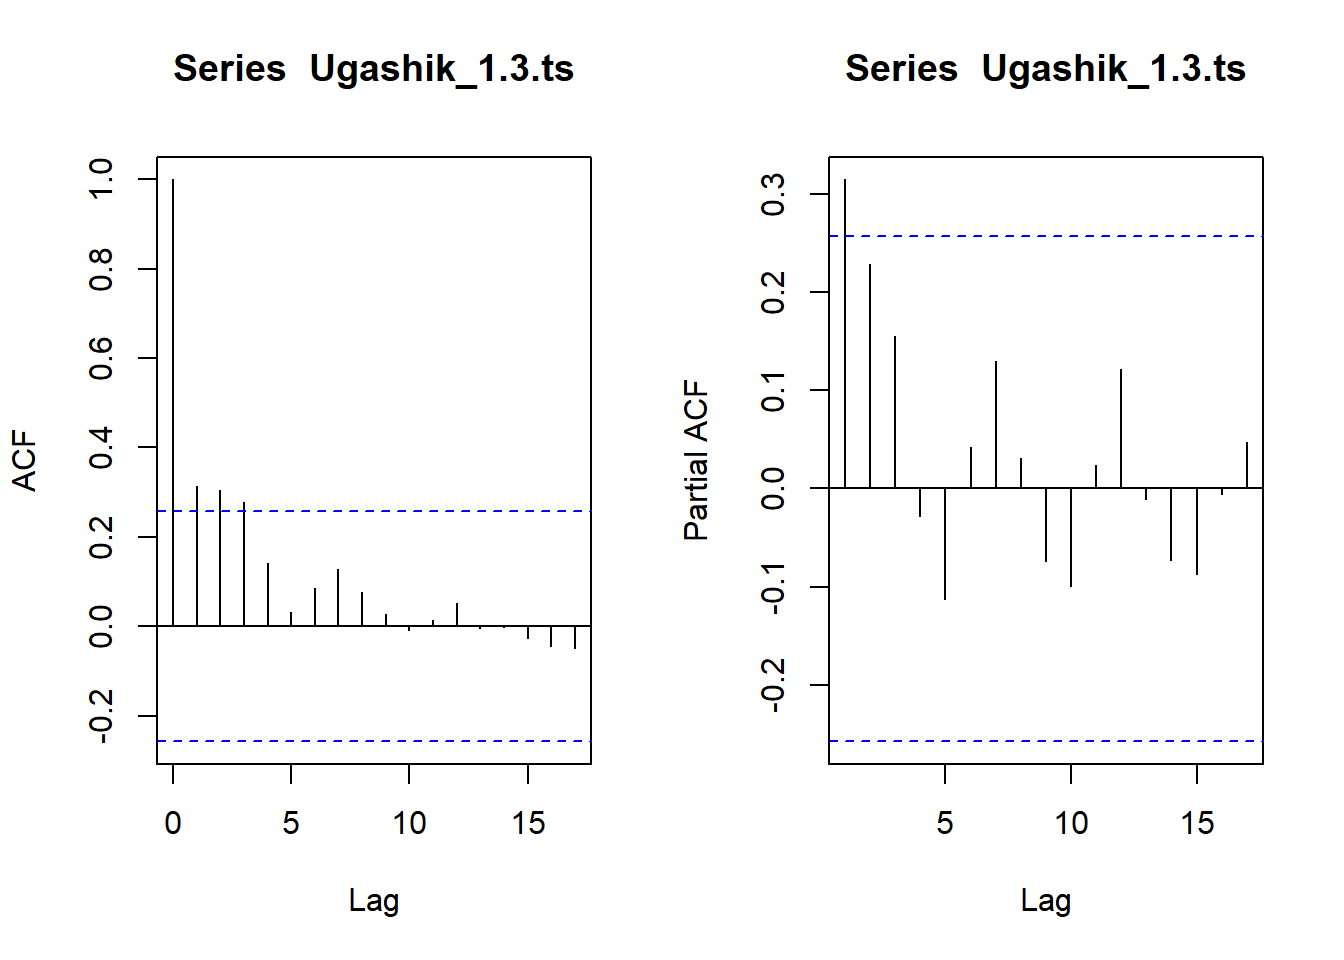
\includegraphics{Lab-1-Emma-ZR-MHS-draft_files/figure-latex/unnamed-chunk-5-1.pdf}
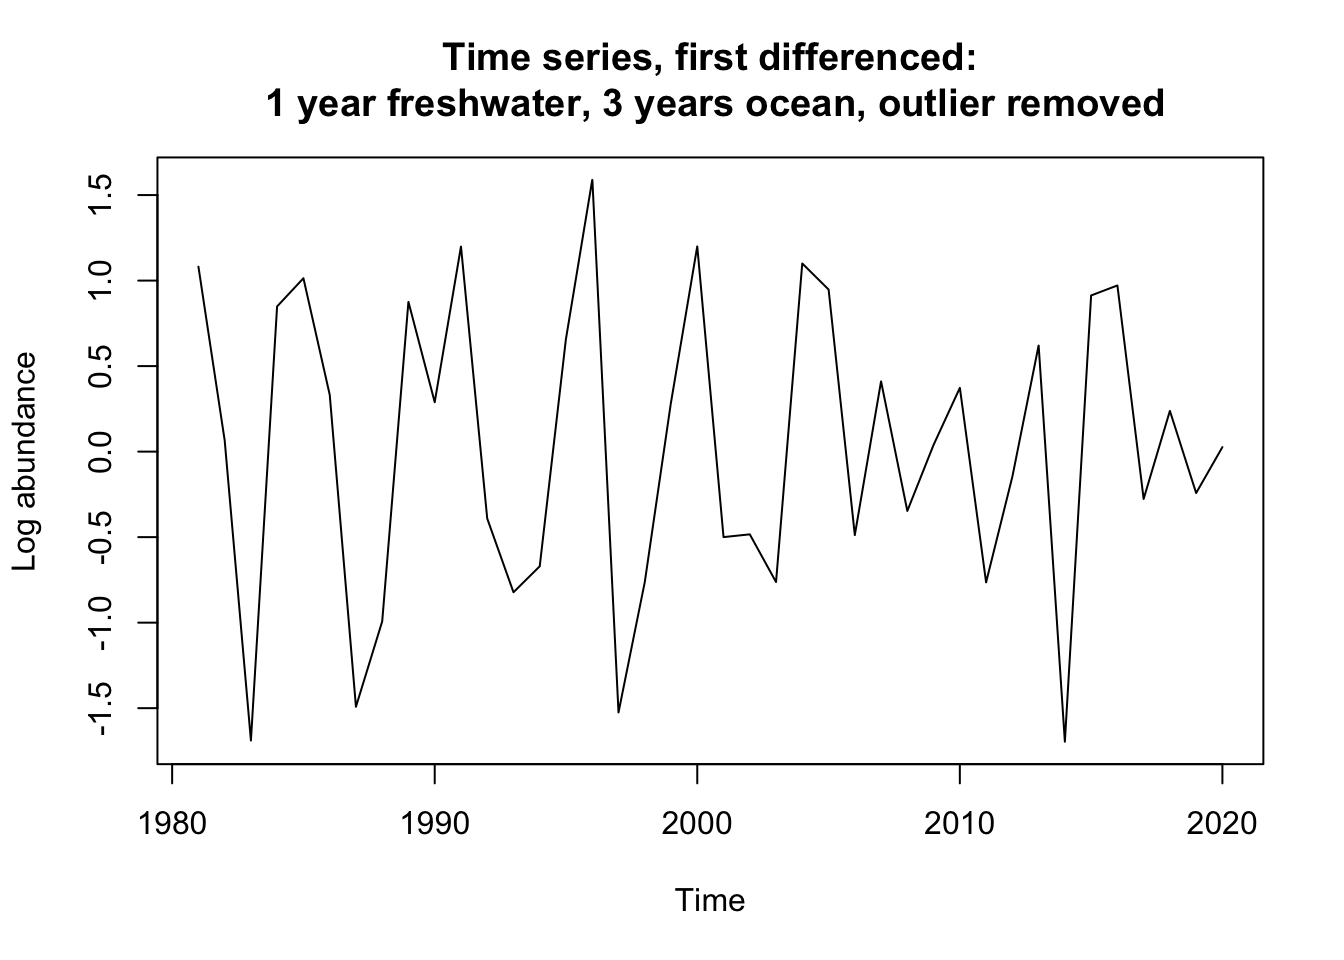
\includegraphics{Lab-1-Emma-ZR-MHS-draft_files/figure-latex/unnamed-chunk-5-2.pdf}

Look at the options for fitting an ARIMA to the data and then choose a
final model. The best model for both of these is ARIMA(0,1,2); however,
a comparison with other models suggests that ARIMA(1,1,1) is also a good
fit with AIC within 0.3 of the ARIMA(0,1,2). The full dataset requires
differencing (d=1).

\begin{Shaded}
\begin{Highlighting}[]
\NormalTok{fit }\OtherTok{\textless{}{-}}\NormalTok{ forecast}\SpecialCharTok{::}\FunctionTok{auto.arima}\NormalTok{(train.sockeye, }\AttributeTok{trace=}\NormalTok{T)}
\end{Highlighting}
\end{Shaded}

\begin{verbatim}
## 
##  ARIMA(2,1,2) with drift         : Inf
##  ARIMA(0,1,0) with drift         : 61.95027
##  ARIMA(1,1,0) with drift         : 60.11204
##  ARIMA(0,1,1) with drift         : 57.27974
##  ARIMA(0,1,0)                    : 59.87487
##  ARIMA(1,1,1) with drift         : Inf
##  ARIMA(0,1,2) with drift         : 57.23854
##  ARIMA(1,1,2) with drift         : Inf
##  ARIMA(0,1,3) with drift         : Inf
##  ARIMA(1,1,3) with drift         : Inf
##  ARIMA(0,1,2)                    : 55.53198
##  ARIMA(0,1,1)                    : 55.33664
##  ARIMA(1,1,1)                    : 55.19379
##  ARIMA(1,1,0)                    : 57.99975
##  ARIMA(2,1,1)                    : 57.46972
##  ARIMA(1,1,2)                    : 57.48549
##  ARIMA(2,1,0)                    : 58.91271
##  ARIMA(2,1,2)                    : Inf
## 
##  Best model: ARIMA(1,1,1)
\end{verbatim}

\begin{Shaded}
\begin{Highlighting}[]
\NormalTok{fit.final.sock}\OtherTok{\textless{}{-}}\NormalTok{forecast}\SpecialCharTok{::}\FunctionTok{auto.arima}\NormalTok{(train.sockeye, }\AttributeTok{approximation =}\NormalTok{ F, }\AttributeTok{stepwise =}\NormalTok{ F)}
\end{Highlighting}
\end{Shaded}

Plot the 5 year forecast for the last part of the dataset compared to
the actual data. The real data are represented by the black dots; the
forecast is represented by the black line.

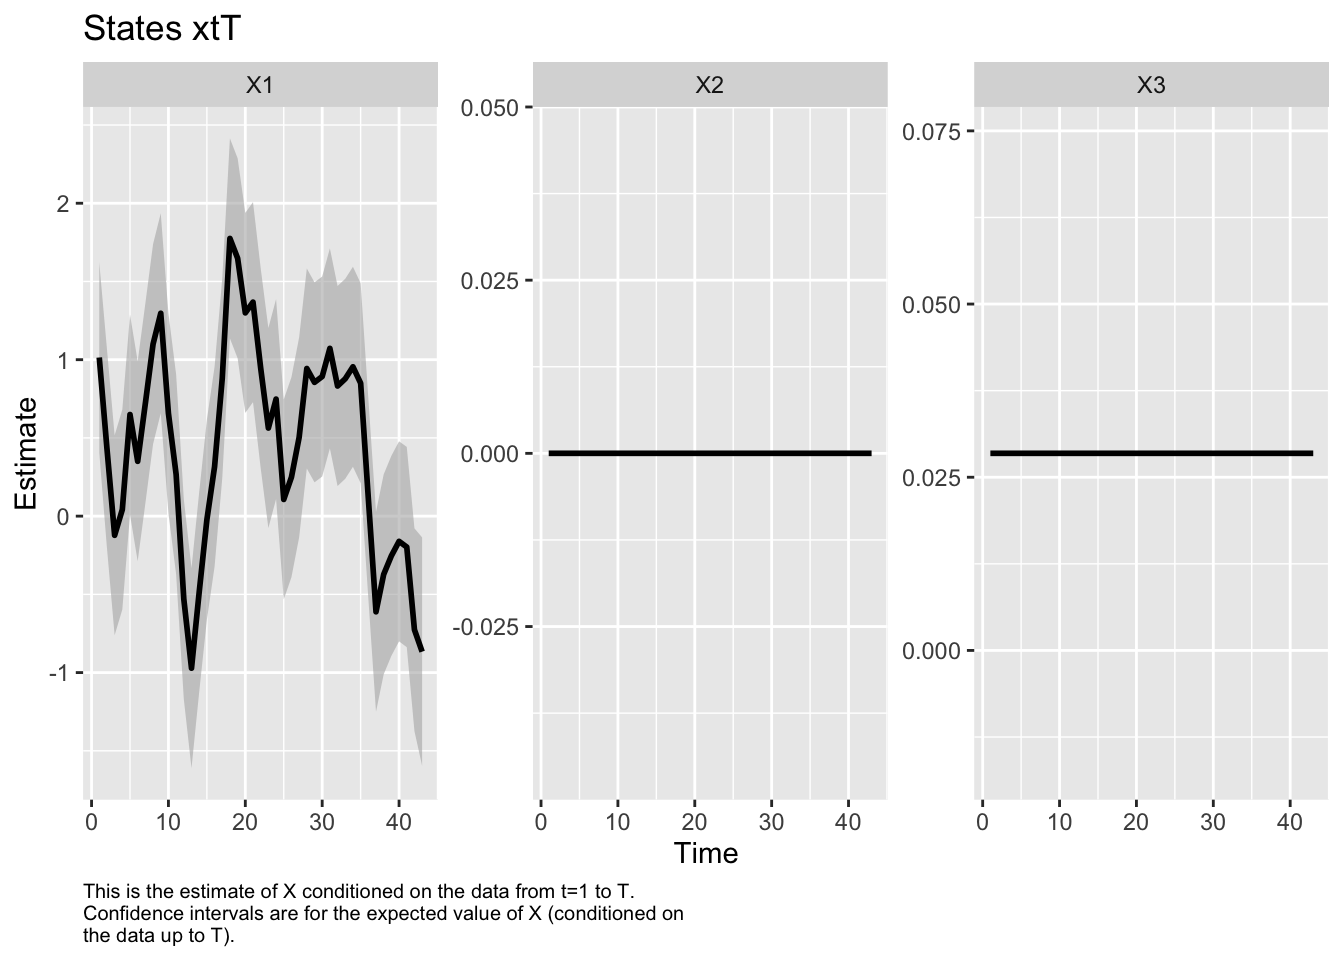
\includegraphics{Lab-1-Emma-ZR-MHS-draft_files/figure-latex/unnamed-chunk-7-1.pdf}

\hypertarget{assess-how-well-forecasting-performs-for-sockeye-returns-by-region}{%
\subsection{Assess how well forecasting performs for sockeye returns by
region}\label{assess-how-well-forecasting-performs-for-sockeye-returns-by-region}}

Create objects needed for plotting.

\begin{Shaded}
\begin{Highlighting}[]
\NormalTok{regions}\OtherTok{\textless{}{-}}\FunctionTok{unique}\NormalTok{(SockByRegion}\SpecialCharTok{$}\NormalTok{region)}
\NormalTok{regionskey}\OtherTok{\textless{}{-}}\FunctionTok{c}\NormalTok{(}\StringTok{"Cook Inlet"}\NormalTok{, }\StringTok{"E. Kamchatka"}\NormalTok{, }\StringTok{"Kodiak"}\NormalTok{, }\StringTok{"Russia"}\NormalTok{, }\StringTok{"N.British Columbia"}\NormalTok{,}
              \StringTok{"Prince William Sound"}\NormalTok{, }\StringTok{"S. Alaska Pen."}\NormalTok{, }\StringTok{"S. British Columbia"}\NormalTok{, }\StringTok{"SE Alaska"}\NormalTok{, }\StringTok{"W. Kamchatka"}\NormalTok{, }\StringTok{"Washington"}\NormalTok{, }\StringTok{"W. Alaska"}\NormalTok{)}
\FunctionTok{names}\NormalTok{(regionskey)}\OtherTok{\textless{}{-}}\NormalTok{regions}
\NormalTok{forecastlevels}\OtherTok{\textless{}{-}}\FunctionTok{c}\NormalTok{(}\DecValTok{5}\NormalTok{, }\DecValTok{10}\NormalTok{, }\DecValTok{20}\NormalTok{)}
\NormalTok{Allcombs}\OtherTok{\textless{}{-}}\FunctionTok{expand\_grid}\NormalTok{(regions, forecastlevels)}
\end{Highlighting}
\end{Shaded}

Plot ACF and PACF for each region.

\begin{Shaded}
\begin{Highlighting}[]
\NormalTok{ACFandPACF}\OtherTok{\textless{}{-}}\ControlFlowTok{function}\NormalTok{(reg)\{}
\NormalTok{  Sockdat}\OtherTok{\textless{}{-}}\NormalTok{SockByRegion }\SpecialCharTok{\%\textgreater{}\%} \FunctionTok{filter}\NormalTok{(region }\SpecialCharTok{==}\NormalTok{ reg)}
  \CommentTok{\#create time series}
\NormalTok{  datts }\OtherTok{\textless{}{-}} \FunctionTok{ts}\NormalTok{(Sockdat}\SpecialCharTok{$}\NormalTok{lnreturns, }\AttributeTok{start=}\NormalTok{Sockdat}\SpecialCharTok{$}\NormalTok{year[}\DecValTok{1}\NormalTok{])}
  \FunctionTok{return}\NormalTok{(}\FunctionTok{list}\NormalTok{(}\AttributeTok{a =} \FunctionTok{acf}\NormalTok{(datts, }\AttributeTok{plot =} \ConstantTok{FALSE}\NormalTok{), }\AttributeTok{p =} \FunctionTok{pacf}\NormalTok{(datts, }\AttributeTok{plot =} \ConstantTok{FALSE}\NormalTok{)))}
\NormalTok{\}}
\end{Highlighting}
\end{Shaded}

\begin{Shaded}
\begin{Highlighting}[]
\NormalTok{DiagPlots}\OtherTok{\textless{}{-}}\FunctionTok{lapply}\NormalTok{(regions, ACFandPACF)}
\FunctionTok{names}\NormalTok{(DiagPlots)}\OtherTok{\textless{}{-}}\NormalTok{regions}
\end{Highlighting}
\end{Shaded}

ACF plots

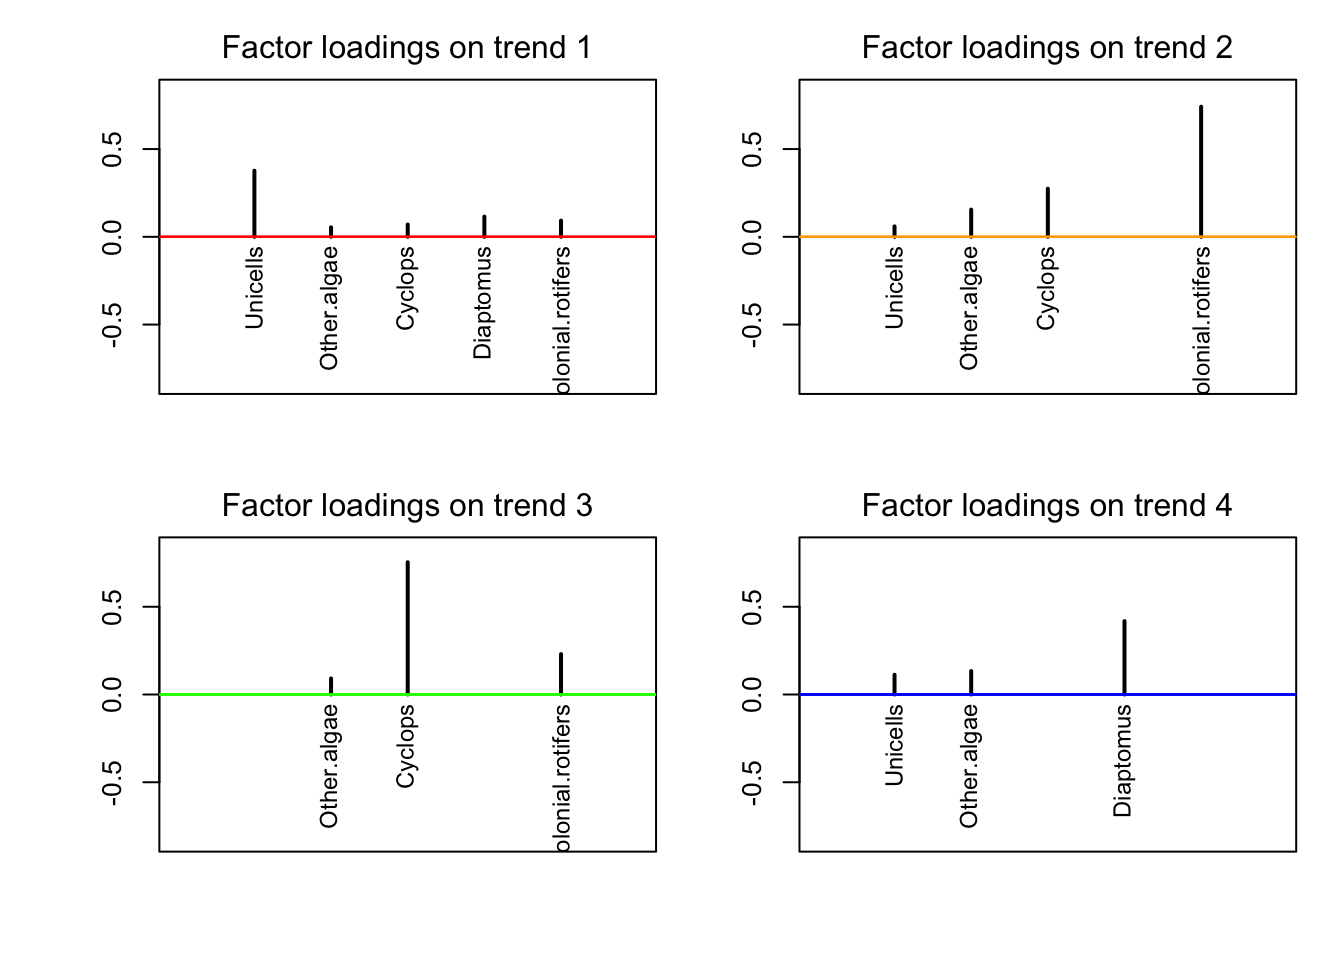
\includegraphics{Lab-1-Emma-ZR-MHS-draft_files/figure-latex/unnamed-chunk-11-1.pdf}

PACF plots

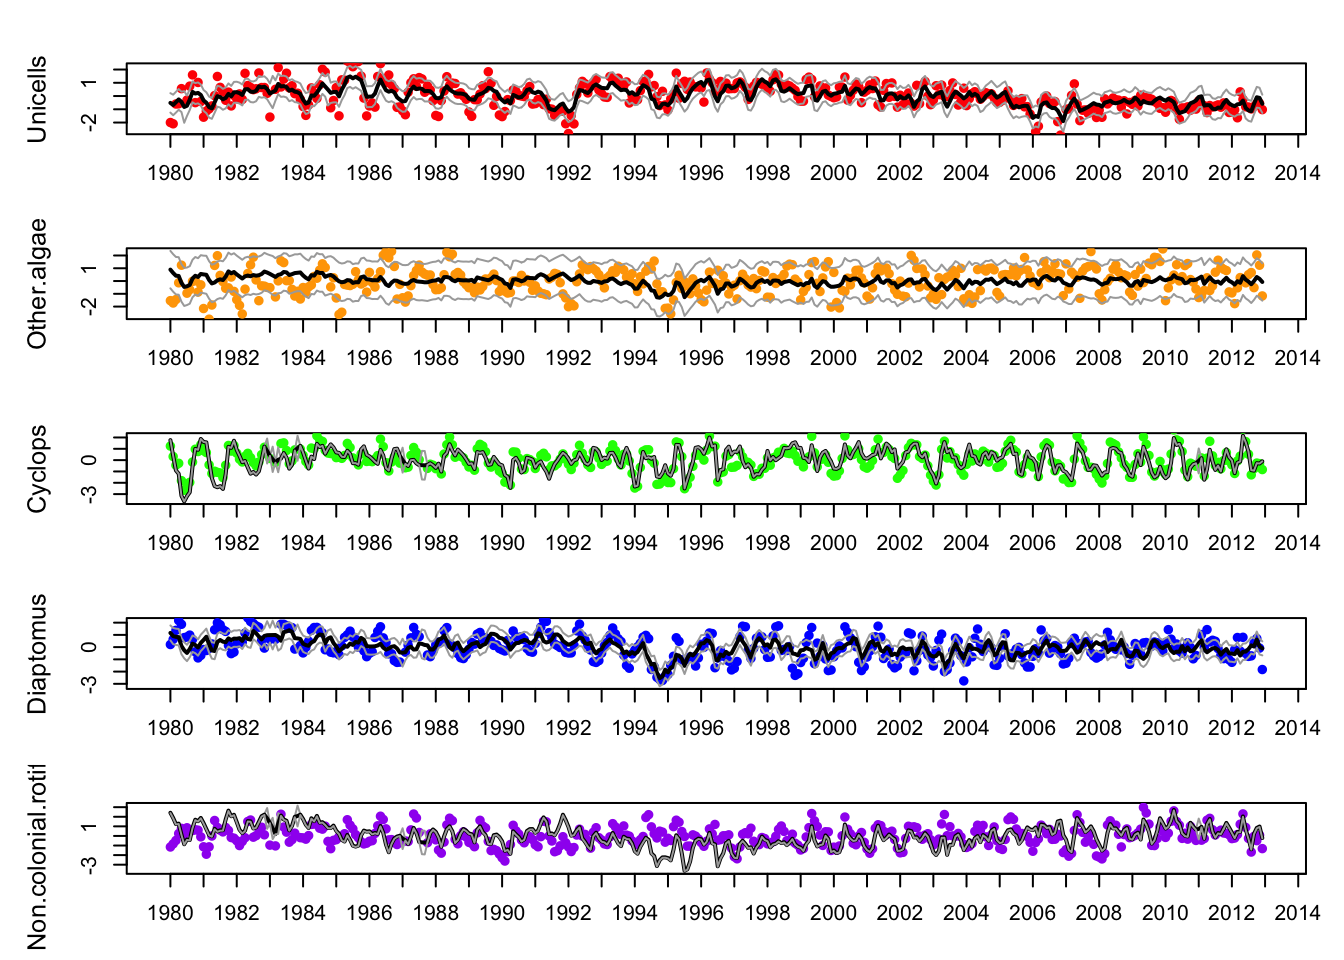
\includegraphics{Lab-1-Emma-ZR-MHS-draft_files/figure-latex/unnamed-chunk-12-1.pdf}

Fit ARIMA models to each region.

\begin{Shaded}
\begin{Highlighting}[]
\NormalTok{FitModFunction}\OtherTok{\textless{}{-}}\ControlFlowTok{function}\NormalTok{(reg, forelevel)\{}
  \CommentTok{\#filter region}
\NormalTok{  Sockdat}\OtherTok{\textless{}{-}}\NormalTok{SockByRegion }\SpecialCharTok{\%\textgreater{}\%} \FunctionTok{filter}\NormalTok{(region }\SpecialCharTok{==}\NormalTok{ reg)}
  \CommentTok{\#create time series}
\NormalTok{  datts }\OtherTok{\textless{}{-}} \FunctionTok{ts}\NormalTok{(Sockdat}\SpecialCharTok{$}\NormalTok{lnreturns, }\AttributeTok{start=}\NormalTok{Sockdat}\SpecialCharTok{$}\NormalTok{year[}\DecValTok{1}\NormalTok{]) }\CommentTok{\#this assumes the first year in data is the start of the time series (they are in order) }
\NormalTok{  cutoff}\OtherTok{\textless{}{-}}\DecValTok{2015}\SpecialCharTok{{-}}\NormalTok{forelevel}
\NormalTok{  train }\OtherTok{\textless{}{-}} \FunctionTok{window}\NormalTok{(datts, }\DecValTok{1952}\NormalTok{, cutoff)}
\NormalTok{  test }\OtherTok{\textless{}{-}} \FunctionTok{window}\NormalTok{(datts, cutoff}\SpecialCharTok{+}\DecValTok{1}\NormalTok{, }\DecValTok{2015}\NormalTok{)}
  
\NormalTok{  mod }\OtherTok{\textless{}{-}} \FunctionTok{auto.arima}\NormalTok{(train)}
  
  \CommentTok{\#testing to be sure that this is the best model (is the best mode the simplest if it is within 2 AIC values?)}
\NormalTok{  trace }\OtherTok{\textless{}{-}} \FunctionTok{capture.output}\NormalTok{(\{}
    \CommentTok{\# assign so it doesn\textquotesingle{}t pollute the output}
\NormalTok{    model }\OtherTok{\textless{}{-}} \FunctionTok{auto.arima}\NormalTok{(datts, }\AttributeTok{trace =} \ConstantTok{TRUE}\NormalTok{)}
\NormalTok{  \})}
\NormalTok{  con    }\OtherTok{\textless{}{-}} \FunctionTok{textConnection}\NormalTok{(trace)}
\NormalTok{  models }\OtherTok{\textless{}{-}} \FunctionTok{read.table}\NormalTok{(con, }\AttributeTok{sep=}\StringTok{":"}\NormalTok{)}
  \FunctionTok{close}\NormalTok{(con)}
  
  \CommentTok{\#getting the "best models" that are within 2 AIC units}
\NormalTok{  BestMods}\OtherTok{\textless{}{-}}\NormalTok{models}\SpecialCharTok{\%\textgreater{}\%} \FunctionTok{filter}\NormalTok{(}\FunctionTok{row\_number}\NormalTok{() }\SpecialCharTok{!=} \FunctionTok{nrow}\NormalTok{(models)) }\SpecialCharTok{\%\textgreater{}\%} \FunctionTok{mutate}\NormalTok{(}\AttributeTok{AIC =} \FunctionTok{replace}\NormalTok{(V2, V2 }\SpecialCharTok{==} \StringTok{"Inf"}\NormalTok{, }\DecValTok{99999}\NormalTok{), }\AttributeTok{AIC =} \FunctionTok{as.numeric}\NormalTok{(AIC), }\AttributeTok{DeltaAIC =}\NormalTok{ AIC}\SpecialCharTok{{-}}\FunctionTok{min}\NormalTok{(AIC)) }\SpecialCharTok{\%\textgreater{}\%} \FunctionTok{filter}\NormalTok{(DeltaAIC }\SpecialCharTok{\textless{}=} \FloatTok{2.0}\NormalTok{)}
  \ControlFlowTok{for}\NormalTok{(i }\ControlFlowTok{in} \DecValTok{1}\SpecialCharTok{:}\FunctionTok{nrow}\NormalTok{(BestMods))\{}
\NormalTok{    BestMods}\SpecialCharTok{$}\NormalTok{Mod[i]}\OtherTok{\textless{}{-}}\FunctionTok{strsplit}\NormalTok{(}\FunctionTok{strsplit}\NormalTok{(}\FunctionTok{strsplit}\NormalTok{(BestMods}\SpecialCharTok{$}\NormalTok{V1[i], }\StringTok{"[(]"}\NormalTok{)[[}\DecValTok{1}\NormalTok{]][}\DecValTok{2}\NormalTok{], }\StringTok{"[)]"}\NormalTok{)[[}\DecValTok{1}\NormalTok{]][}\DecValTok{1}\NormalTok{],}\StringTok{"[,]"}\NormalTok{)}
\NormalTok{    BestMods}\SpecialCharTok{$}\NormalTok{npar[i]}\OtherTok{\textless{}{-}}\FunctionTok{sum}\NormalTok{(}\FunctionTok{as.numeric}\NormalTok{(BestMods}\SpecialCharTok{$}\NormalTok{Mod[i][[}\DecValTok{1}\NormalTok{]][}\FunctionTok{c}\NormalTok{(}\DecValTok{1}\NormalTok{,}\DecValTok{3}\NormalTok{)]))}
    \ControlFlowTok{if}\NormalTok{(}\FunctionTok{strsplit}\NormalTok{(}\FunctionTok{strsplit}\NormalTok{(BestMods}\SpecialCharTok{$}\NormalTok{V1[i], }\StringTok{"[(]"}\NormalTok{)[[}\DecValTok{1}\NormalTok{]][}\DecValTok{2}\NormalTok{], }\StringTok{"[)]"}\NormalTok{)[[}\DecValTok{1}\NormalTok{]][}\DecValTok{2}\NormalTok{] }\SpecialCharTok{==} \StringTok{" with drift         "}\NormalTok{)\{}
\NormalTok{      BestMods}\SpecialCharTok{$}\NormalTok{npar[i] }\OtherTok{=}\NormalTok{ BestMods}\SpecialCharTok{$}\NormalTok{npar[i] }\SpecialCharTok{+} \DecValTok{1}
\NormalTok{    \}}
\NormalTok{  \}}
  
\NormalTok{  New}\OtherTok{\textless{}{-}}\NormalTok{BestMods }\SpecialCharTok{\%\textgreater{}\%} \FunctionTok{filter}\NormalTok{(npar }\SpecialCharTok{==} \FunctionTok{min}\NormalTok{(npar))}
  \ControlFlowTok{if}\NormalTok{(}\DecValTok{0} \SpecialCharTok{\%in\%}\NormalTok{ New}\SpecialCharTok{$}\NormalTok{DeltaAIC)\{}
      \CommentTok{\#auto arima picked the best model}
\NormalTok{      res}\OtherTok{\textless{}{-}}\FunctionTok{accuracy}\NormalTok{(}\FunctionTok{forecast}\NormalTok{(mod, }\AttributeTok{h=}\NormalTok{forelevel), test)[}\DecValTok{2}\NormalTok{,}\StringTok{"MASE"}\NormalTok{] }\CommentTok{\#test set MASE}
\NormalTok{  \}}\ControlFlowTok{else}\NormalTok{\{}
      \CommentTok{\#of the models with the fewest parameters, pick the lowest AIC}
\NormalTok{      newmod}\OtherTok{\textless{}{-}}\NormalTok{New }\SpecialCharTok{\%\textgreater{}\%} \FunctionTok{filter}\NormalTok{(AIC }\SpecialCharTok{==} \FunctionTok{min}\NormalTok{(AIC)) }\SpecialCharTok{\%\textgreater{}\%} \FunctionTok{select}\NormalTok{(Mod)}
\NormalTok{      mod}\OtherTok{\textless{}{-}}\FunctionTok{Arima}\NormalTok{(train, }\AttributeTok{order =} \FunctionTok{as.numeric}\NormalTok{(}\FunctionTok{strsplit}\NormalTok{(newmod}\SpecialCharTok{$}\NormalTok{Mod[[}\DecValTok{1}\NormalTok{]], }\StringTok{"[,]"}\NormalTok{)), }\AttributeTok{include.constant =} \ConstantTok{TRUE}\NormalTok{)}
\NormalTok{      res}\OtherTok{\textless{}{-}}\FunctionTok{accuracy}\NormalTok{(}\FunctionTok{forecast}\NormalTok{(mod, }\AttributeTok{h=}\NormalTok{forelevel), test)[}\DecValTok{2}\NormalTok{,}\StringTok{"MASE"}\NormalTok{] }\CommentTok{\#test set MASE}
\NormalTok{    \}}

  \FunctionTok{return}\NormalTok{(}\FunctionTok{list}\NormalTok{(}\AttributeTok{Fit =}\NormalTok{ mod, }\AttributeTok{MASE =}\NormalTok{ res, }\AttributeTok{Bm =}\NormalTok{ BestMods)) }\CommentTok{\#include best mods for testing to see that it\textquotesingle{}s doing what I want}
\NormalTok{\}}
\NormalTok{RegionModsSock}\OtherTok{\textless{}{-}}\FunctionTok{mapply}\NormalTok{(FitModFunction, Allcombs}\SpecialCharTok{$}\NormalTok{regions, Allcombs}\SpecialCharTok{$}\NormalTok{forecastlevels, }\AttributeTok{SIMPLIFY =} \ConstantTok{FALSE}\NormalTok{)}
\end{Highlighting}
\end{Shaded}

Extract MASE for comparisons of models across regions.

\begin{Shaded}
\begin{Highlighting}[]
\NormalTok{RegionMASESock}\OtherTok{\textless{}{-}}\FunctionTok{sapply}\NormalTok{(RegionModsSock, }\ControlFlowTok{function}\NormalTok{(x)\{y}\OtherTok{\textless{}{-}}\NormalTok{x}\SpecialCharTok{$}\NormalTok{MASE\})}
\NormalTok{RegionBestModSock}\OtherTok{\textless{}{-}}\FunctionTok{sapply}\NormalTok{(RegionModsSock, }\ControlFlowTok{function}\NormalTok{(x)\{y}\OtherTok{\textless{}{-}}\FunctionTok{as.character}\NormalTok{(x}\SpecialCharTok{$}\NormalTok{Fit)\})}

\NormalTok{ResultsTableSock}\OtherTok{\textless{}{-}}\NormalTok{Allcombs }\SpecialCharTok{\%\textgreater{}\%} \FunctionTok{add\_column}\NormalTok{(}\AttributeTok{Model =}\NormalTok{ RegionBestModSock, }\AttributeTok{MASE =}\NormalTok{ RegionMASESock)}
\end{Highlighting}
\end{Shaded}

How well does auto.arima do in choosing a model? Is it different from
what we would choose looking at ACF and PACF? For Cook Inlet, auto.arima
selected ARIMA(4,1,1), but PACF has a significant lag at 6 and ACF
trails off.

\begin{Shaded}
\begin{Highlighting}[]
\NormalTok{sock.ci}\OtherTok{\textless{}{-}}\FunctionTok{subset}\NormalTok{(SockByRegion, region}\SpecialCharTok{==}\StringTok{\textquotesingle{}ci\textquotesingle{}}\NormalTok{)}
\NormalTok{ci.ts}\OtherTok{\textless{}{-}}\FunctionTok{ts}\NormalTok{(sock.ci}\SpecialCharTok{$}\NormalTok{lnreturns, }\AttributeTok{start=}\NormalTok{sock.ci}\SpecialCharTok{$}\NormalTok{year[}\DecValTok{1}\NormalTok{])}
\NormalTok{forecast}\SpecialCharTok{::}\FunctionTok{ndiffs}\NormalTok{(ci.ts, }\AttributeTok{test=}\StringTok{\textquotesingle{}adf\textquotesingle{}}\NormalTok{)}
\end{Highlighting}
\end{Shaded}

\begin{verbatim}
## [1] 1
\end{verbatim}

\begin{Shaded}
\begin{Highlighting}[]
\NormalTok{forecast}\SpecialCharTok{::}\FunctionTok{ndiffs}\NormalTok{(ci.ts, }\AttributeTok{test=}\StringTok{\textquotesingle{}kpss\textquotesingle{}}\NormalTok{)}
\end{Highlighting}
\end{Shaded}

\begin{verbatim}
## [1] 1
\end{verbatim}

\begin{Shaded}
\begin{Highlighting}[]
\NormalTok{train.ci5}\OtherTok{\textless{}{-}}\FunctionTok{window}\NormalTok{(ci.ts, }\AttributeTok{start=}\DecValTok{1952}\NormalTok{, }\AttributeTok{end=}\DecValTok{2010}\NormalTok{)}
\NormalTok{test.ci5}\OtherTok{\textless{}{-}}\FunctionTok{window}\NormalTok{(ci.ts, }\AttributeTok{start=}\DecValTok{2011}\NormalTok{, }\AttributeTok{end=}\DecValTok{2015}\NormalTok{)}
\NormalTok{ci.final5}\OtherTok{\textless{}{-}}\NormalTok{forecast}\SpecialCharTok{::}\FunctionTok{auto.arima}\NormalTok{(train.ci5, }\AttributeTok{approximation =}\NormalTok{ F, }\AttributeTok{stepwise =}\NormalTok{ F)}
\FunctionTok{accuracy}\NormalTok{(}\FunctionTok{forecast}\NormalTok{(ci.final5, }\AttributeTok{h=}\DecValTok{5}\NormalTok{), test.ci5)}
\end{Highlighting}
\end{Shaded}

\begin{verbatim}
##                      ME      RMSE       MAE       MPE     MAPE      MASE
## Training set 0.02471079 0.3370305 0.2702999 -38.06705 62.87923 0.8967555
## Test set     0.34919358 0.4082214 0.3491936  17.84353 17.84353 1.1584957
##                      ACF1 Theil's U
## Training set  0.008040561        NA
## Test set     -0.080588177  1.829245
\end{verbatim}

\begin{Shaded}
\begin{Highlighting}[]
\CommentTok{\#MASE is just above 1}

\FunctionTok{acf}\NormalTok{(train.ci5)}
\end{Highlighting}
\end{Shaded}

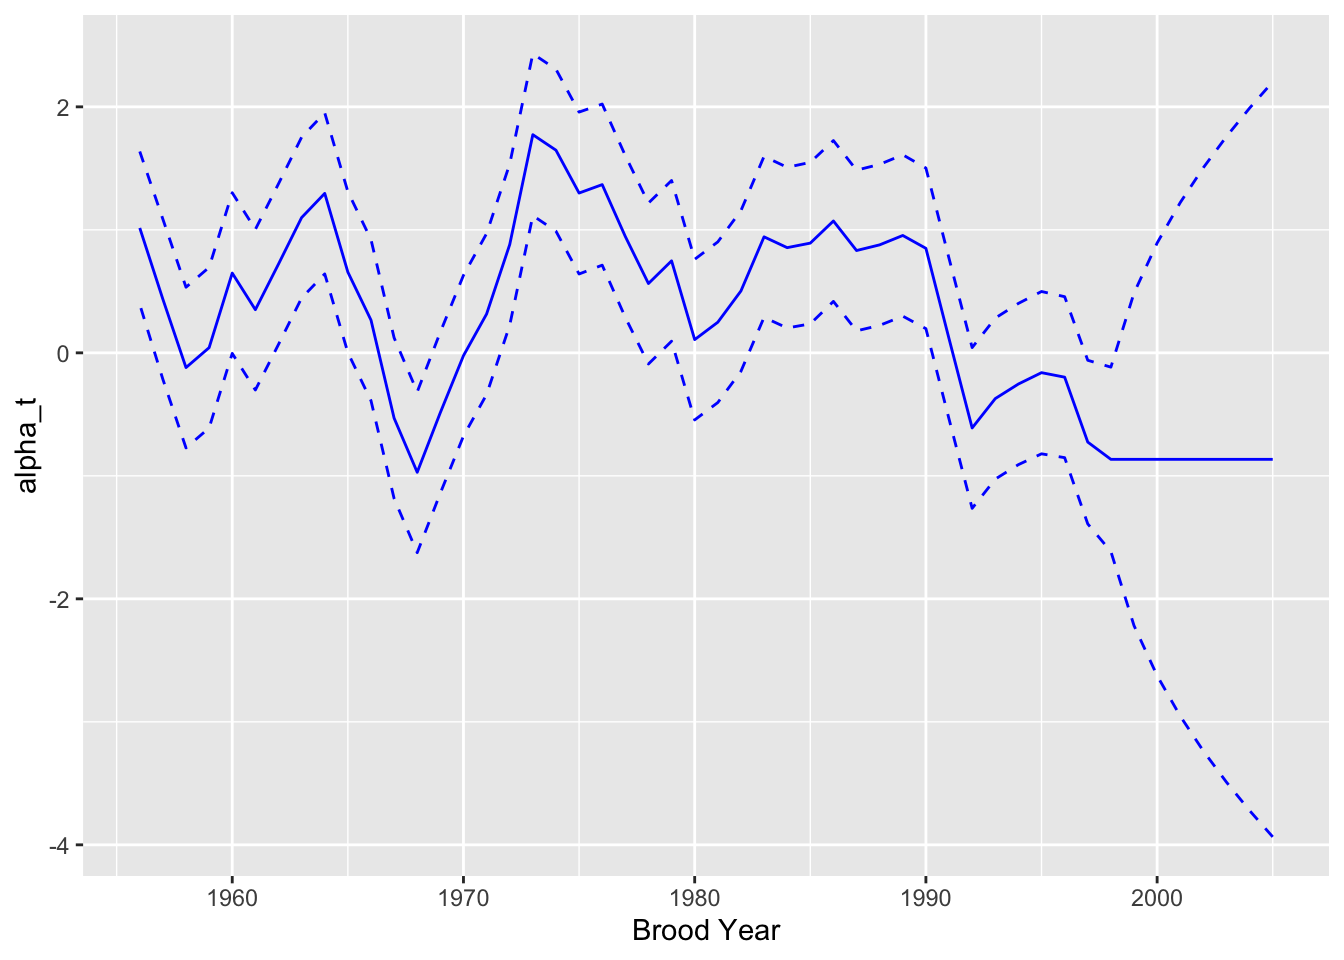
\includegraphics{Lab-1-Emma-ZR-MHS-draft_files/figure-latex/unnamed-chunk-15-1.pdf}

\begin{Shaded}
\begin{Highlighting}[]
\FunctionTok{pacf}\NormalTok{(train.ci5)}
\end{Highlighting}
\end{Shaded}

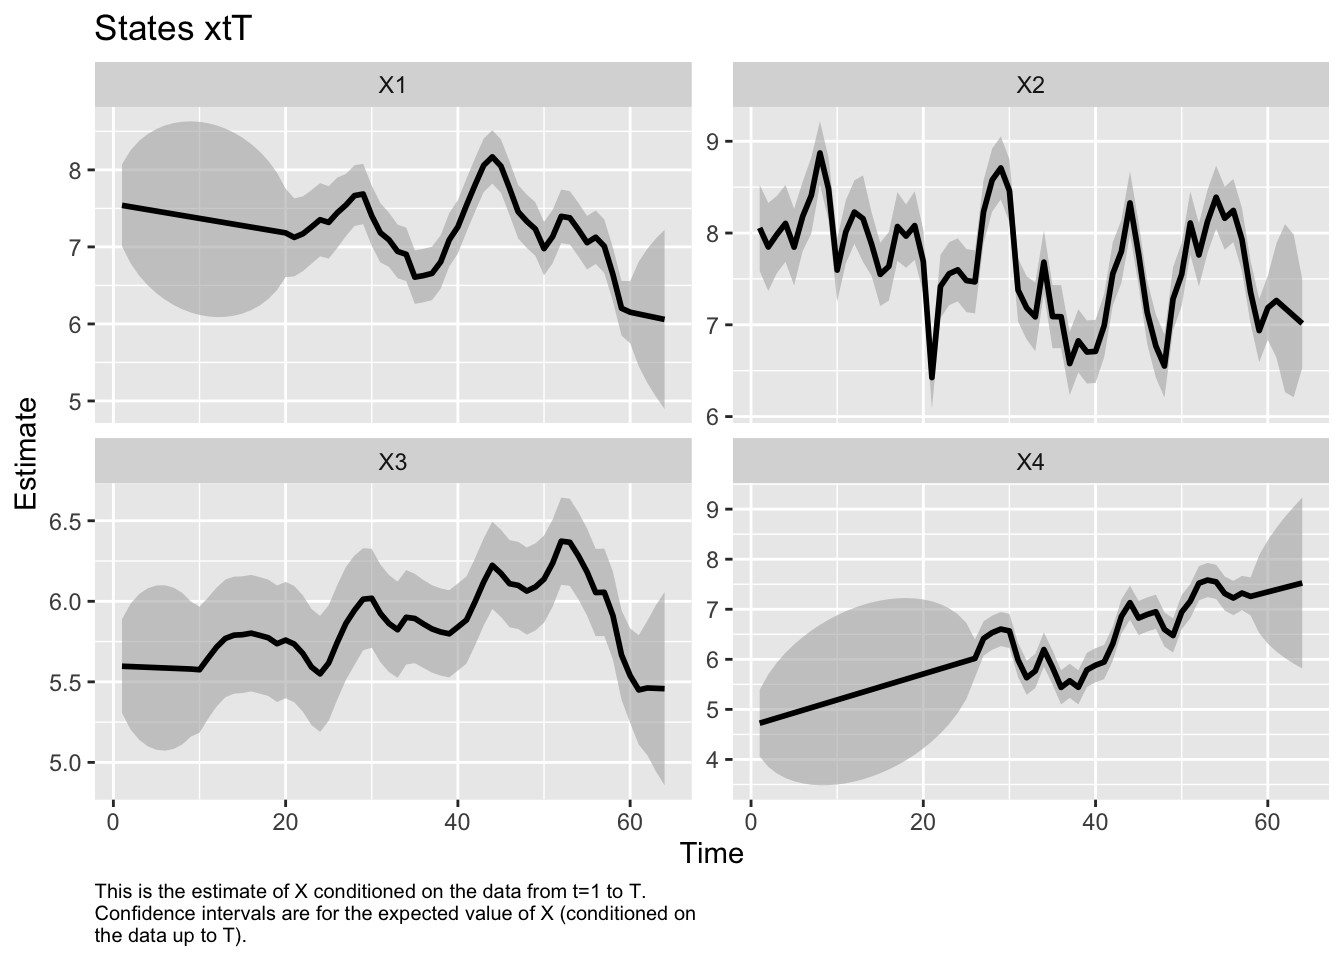
\includegraphics{Lab-1-Emma-ZR-MHS-draft_files/figure-latex/unnamed-chunk-15-2.pdf}

\begin{Shaded}
\begin{Highlighting}[]
\CommentTok{\#select ARIMA (6,1,0)}
\NormalTok{fit.ci2 }\OtherTok{\textless{}{-}} \FunctionTok{Arima}\NormalTok{(train.ci5, }\AttributeTok{order=}\FunctionTok{c}\NormalTok{(}\DecValTok{6}\NormalTok{,}\DecValTok{1}\NormalTok{,}\DecValTok{0}\NormalTok{), }\AttributeTok{include.mean=}\ConstantTok{TRUE}\NormalTok{)}
\FunctionTok{accuracy}\NormalTok{(}\FunctionTok{forecast}\NormalTok{(fit, }\AttributeTok{h=}\DecValTok{5}\NormalTok{), test.ci5)}
\end{Highlighting}
\end{Shaded}

\begin{verbatim}
##                      ME      RMSE       MAE       MPE     MAPE      MASE
## Training set 0.03439583 0.3641608 0.2787817 -40.97753 65.59960 0.9248951
## Test set     0.29776606 0.3308204 0.2977661  15.30517 15.30517 0.9878781
##                      ACF1 Theil's U
## Training set -0.007356741        NA
## Test set      0.206715703  1.669537
\end{verbatim}

\begin{Shaded}
\begin{Highlighting}[]
\CommentTok{\#MASE is very high for the test set.}
\end{Highlighting}
\end{Shaded}

Here are the plots comparing the two models for Cook Inlet. The plots
look very similar, but the forecast differs a bit for the last 2 years.

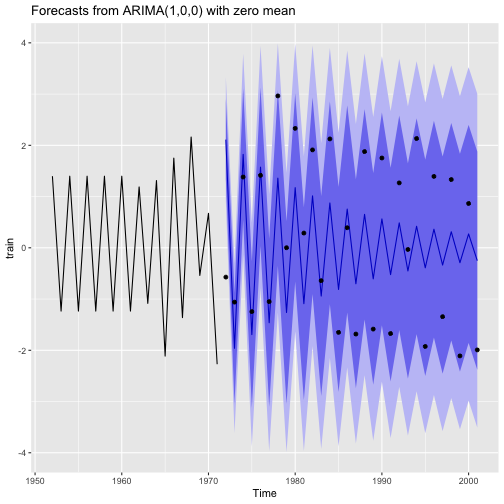
\includegraphics{Lab-1-Emma-ZR-MHS-draft_files/figure-latex/unnamed-chunk-16-1.pdf}
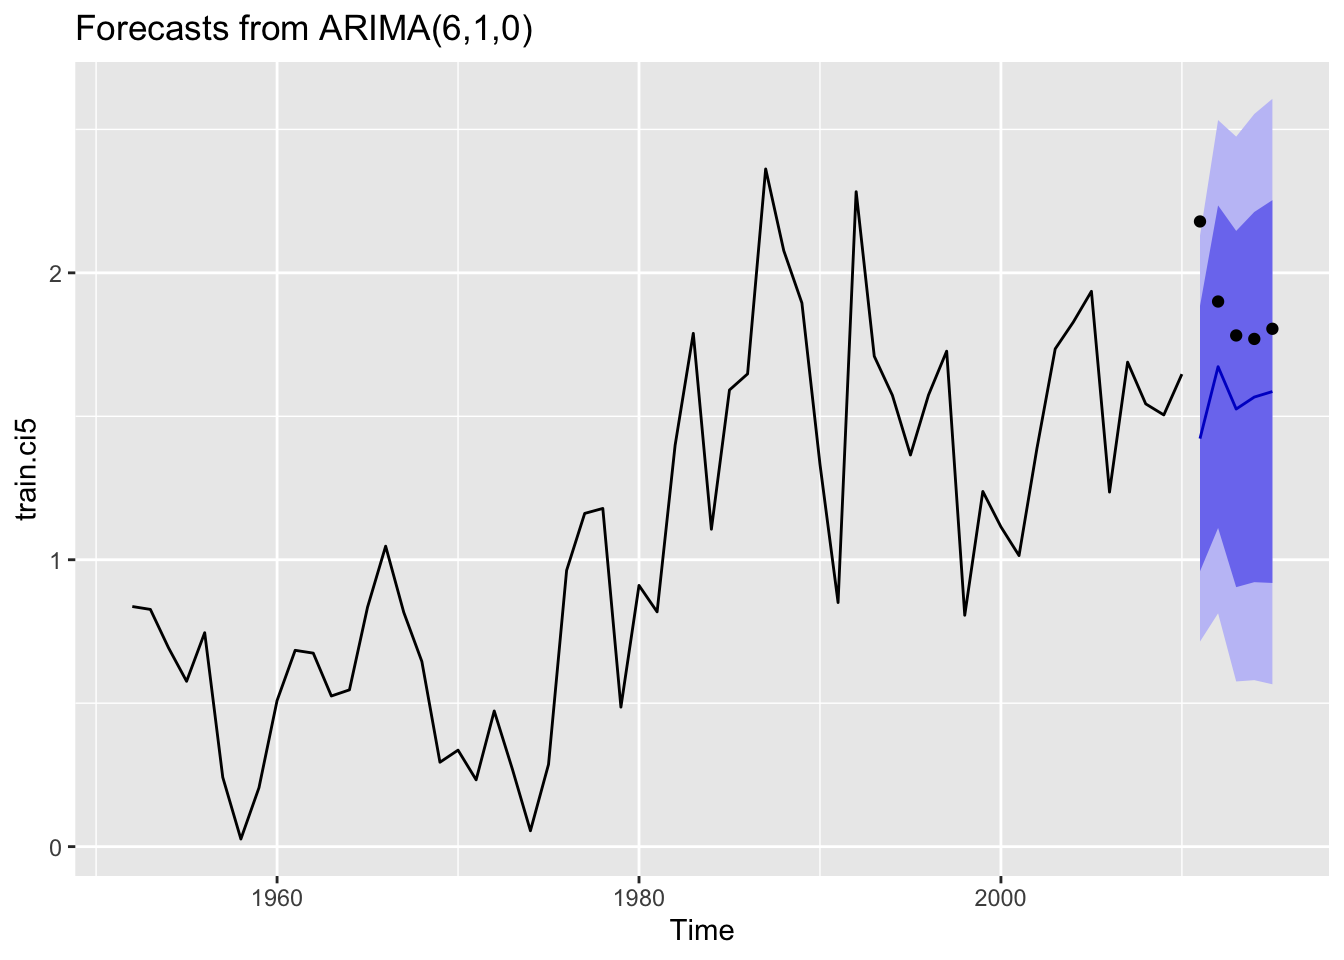
\includegraphics{Lab-1-Emma-ZR-MHS-draft_files/figure-latex/unnamed-chunk-16-2.pdf}

\hypertarget{chum-regional}{%
\subsection{Chum: Regional}\label{chum-regional}}

Looking at data:

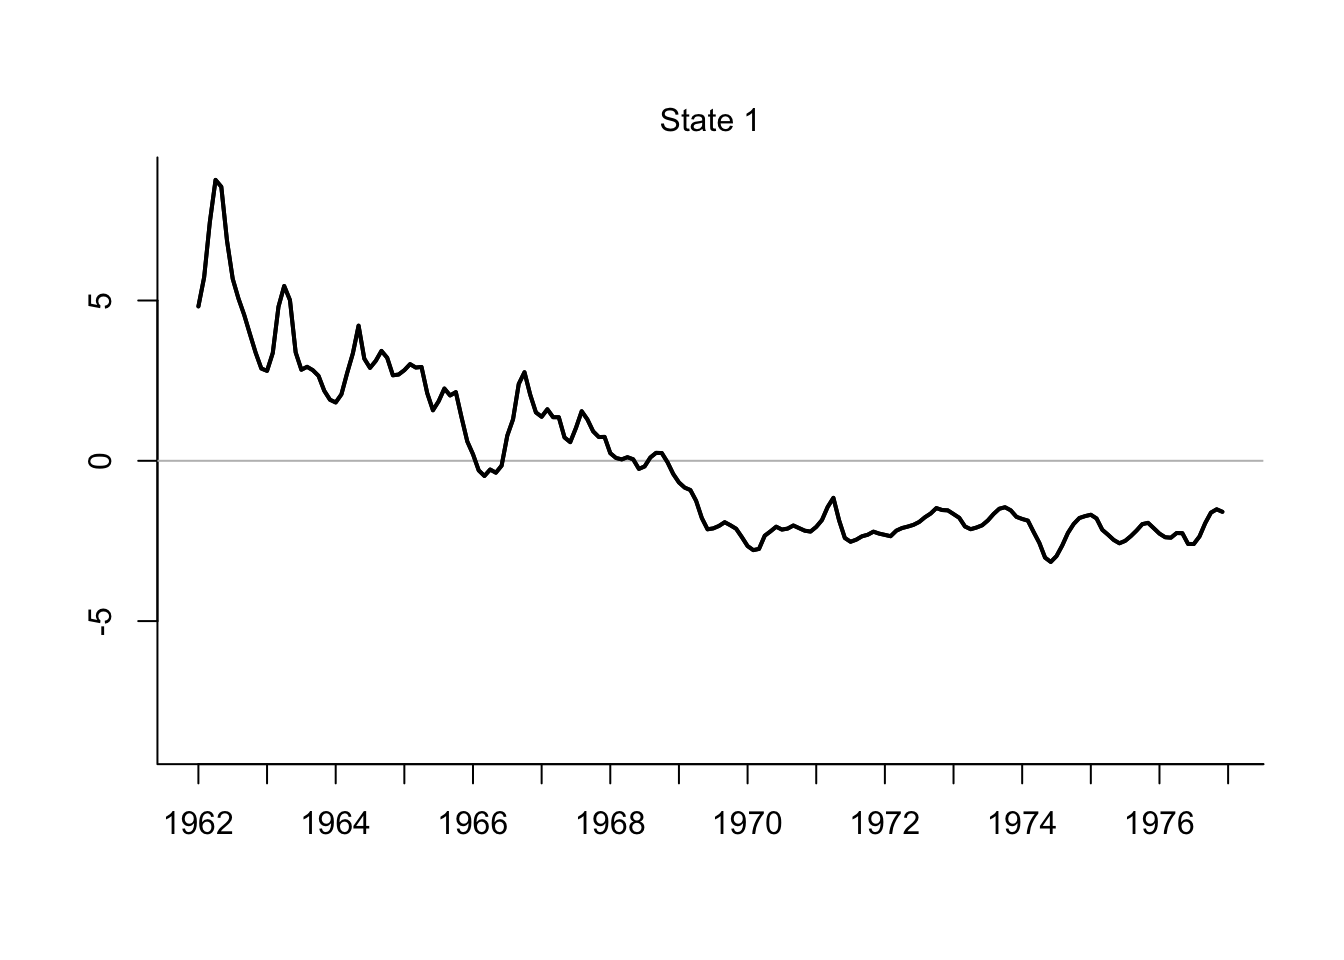
\includegraphics{Lab-1-Emma-ZR-MHS-draft_files/figure-latex/unnamed-chunk-17-1.pdf}

Getting a subset of the data (removing regions with no data):

\begin{Shaded}
\begin{Highlighting}[]
\CommentTok{\#removing Korea Japan because there\textquotesingle{}s no data}
\NormalTok{ChumByRegion}\OtherTok{\textless{}{-}}\NormalTok{ruggerone\_data }\SpecialCharTok{\%\textgreater{}\%}
  \FunctionTok{filter}\NormalTok{(region }\SpecialCharTok{!=} \StringTok{"japan"}\NormalTok{) }\SpecialCharTok{\%\textgreater{}\%}
  \FunctionTok{filter}\NormalTok{(region }\SpecialCharTok{!=} \StringTok{"korea"}\NormalTok{) }\SpecialCharTok{\%\textgreater{}\%}
  \FunctionTok{group\_by}\NormalTok{(species, region, year) }\SpecialCharTok{\%\textgreater{}\%}
  \FunctionTok{summarize}\NormalTok{(}\AttributeTok{total =} \FunctionTok{sum}\NormalTok{(returns, }\AttributeTok{na.rm=}\ConstantTok{TRUE}\NormalTok{)) }\SpecialCharTok{\%\textgreater{}\%} 
  \FunctionTok{mutate}\NormalTok{(}\AttributeTok{lnreturns =} \FunctionTok{log}\NormalTok{(total)) }\SpecialCharTok{\%\textgreater{}\%}
  \FunctionTok{filter}\NormalTok{(species }\SpecialCharTok{==} \StringTok{"chum"}\NormalTok{)}
\end{Highlighting}
\end{Shaded}

\begin{verbatim}
## `summarise()` has grouped output by 'species', 'region'. You can override using
## the `.groups` argument.
\end{verbatim}

\begin{Shaded}
\begin{Highlighting}[]
\FunctionTok{head}\NormalTok{(ChumByRegion)}
\end{Highlighting}
\end{Shaded}

\begin{verbatim}
## # A tibble: 6 x 5
## # Groups:   species, region [1]
##   species region  year total lnreturns
##   <chr>   <chr>  <dbl> <dbl>     <dbl>
## 1 chum    ci      1952 1.25     0.226 
## 2 chum    ci      1953 1.44     0.363 
## 3 chum    ci      1954 1.93     0.656 
## 4 chum    ci      1955 0.957   -0.0436
## 5 chum    ci      1956 2.11     0.748 
## 6 chum    ci      1957 2.76     1.01
\end{verbatim}

\begin{Shaded}
\begin{Highlighting}[]
\CommentTok{\#making sure all the regions cover all the years (or at least start and end)}
\NormalTok{ChumByRegion }\SpecialCharTok{\%\textgreater{}\%} \FunctionTok{group\_by}\NormalTok{(region) }\SpecialCharTok{\%\textgreater{}\%} \FunctionTok{summarise}\NormalTok{(}\AttributeTok{startyear =} \FunctionTok{min}\NormalTok{(year), }\AttributeTok{endyear =} \FunctionTok{max}\NormalTok{(year))}
\end{Highlighting}
\end{Shaded}

\begin{verbatim}
## # A tibble: 12 x 3
##    region startyear endyear
##    <chr>      <dbl>   <dbl>
##  1 ci          1952    2015
##  2 e_kam       1952    2015
##  3 kod         1952    2015
##  4 m_i         1952    2015
##  5 nbc         1952    2015
##  6 pws         1952    2015
##  7 s_pen       1952    2015
##  8 sbc         1952    2015
##  9 seak        1952    2015
## 10 w_kam       1952    2015
## 11 wa          1952    2015
## 12 wak         1952    2015
\end{verbatim}

\begin{Shaded}
\begin{Highlighting}[]
\CommentTok{\#all start in 1952 and end in 2015}
\end{Highlighting}
\end{Shaded}

Creating tibble to loop through:

\begin{Shaded}
\begin{Highlighting}[]
\CommentTok{\#regions vector}
\NormalTok{regions}\OtherTok{\textless{}{-}}\FunctionTok{unique}\NormalTok{(ChumByRegion}\SpecialCharTok{$}\NormalTok{region)}
\CommentTok{\#regions key}
\NormalTok{regionskey}\OtherTok{\textless{}{-}}\FunctionTok{c}\NormalTok{(}\StringTok{"Cook Inlet"}\NormalTok{, }\StringTok{"E. Kamchatka"}\NormalTok{, }\StringTok{"Kodiak"}\NormalTok{, }\StringTok{"Russia"}\NormalTok{, }\StringTok{"N.British Columbia"}\NormalTok{,}
              \StringTok{"Prince William Sound"}\NormalTok{, }\StringTok{"S. Alaska Pen."}\NormalTok{, }\StringTok{"S. British Columbia"}\NormalTok{, }\StringTok{"SE Alaska"}\NormalTok{, }\StringTok{"W. Kamchatka"}\NormalTok{, }\StringTok{"Washington"}\NormalTok{, }\StringTok{"W. Alaska"}\NormalTok{)}
\FunctionTok{names}\NormalTok{(regionskey)}\OtherTok{\textless{}{-}}\NormalTok{regions }\CommentTok{\#for plotting}
\CommentTok{\#forecast levels}
\NormalTok{forecastlevels}\OtherTok{\textless{}{-}}\FunctionTok{c}\NormalTok{(}\DecValTok{5}\NormalTok{, }\DecValTok{10}\NormalTok{, }\DecValTok{20}\NormalTok{)}
\CommentTok{\#all combinations}
\NormalTok{Allcombs}\OtherTok{\textless{}{-}}\FunctionTok{expand\_grid}\NormalTok{(regions, forecastlevels)}
\end{Highlighting}
\end{Shaded}

Function for ACF and PACF

\begin{Shaded}
\begin{Highlighting}[]
\CommentTok{\#ACF and PACF}
\NormalTok{ACFandPACF}\OtherTok{\textless{}{-}}\ControlFlowTok{function}\NormalTok{(reg)\{}
\NormalTok{  Chumdat}\OtherTok{\textless{}{-}}\NormalTok{ChumByRegion }\SpecialCharTok{\%\textgreater{}\%} \FunctionTok{filter}\NormalTok{(region }\SpecialCharTok{==}\NormalTok{ reg)}
  \CommentTok{\#create time series}
\NormalTok{  datts }\OtherTok{\textless{}{-}} \FunctionTok{ts}\NormalTok{(Chumdat}\SpecialCharTok{$}\NormalTok{lnreturns, }\AttributeTok{start=}\NormalTok{Chumdat}\SpecialCharTok{$}\NormalTok{year[}\DecValTok{1}\NormalTok{])}
  \FunctionTok{return}\NormalTok{(}\FunctionTok{list}\NormalTok{(}\AttributeTok{a =} \FunctionTok{acf}\NormalTok{(datts, }\AttributeTok{plot =} \ConstantTok{FALSE}\NormalTok{), }\AttributeTok{p =} \FunctionTok{pacf}\NormalTok{(datts, }\AttributeTok{plot =} \ConstantTok{FALSE}\NormalTok{)))}
\NormalTok{\}}
\CommentTok{\#loop through regions/levels}
\NormalTok{DiagPlots}\OtherTok{\textless{}{-}}\FunctionTok{lapply}\NormalTok{(regions, ACFandPACF)}
\FunctionTok{names}\NormalTok{(DiagPlots)}\OtherTok{\textless{}{-}}\NormalTok{regions}
\end{Highlighting}
\end{Shaded}

\begin{Shaded}
\begin{Highlighting}[]
\CommentTok{\#ACF plots for each region}
\FunctionTok{par}\NormalTok{(}\AttributeTok{mfrow=}\FunctionTok{c}\NormalTok{(}\DecValTok{3}\NormalTok{,}\DecValTok{4}\NormalTok{))}
\ControlFlowTok{for}\NormalTok{(r }\ControlFlowTok{in} \DecValTok{1}\SpecialCharTok{:}\FunctionTok{length}\NormalTok{(regions))\{}
  \FunctionTok{plot}\NormalTok{(DiagPlots[[r]][[}\DecValTok{1}\NormalTok{]], }\AttributeTok{main =} \FunctionTok{paste0}\NormalTok{(}\StringTok{"Region: "}\NormalTok{, regionskey[r]))}
\NormalTok{\}}
\end{Highlighting}
\end{Shaded}

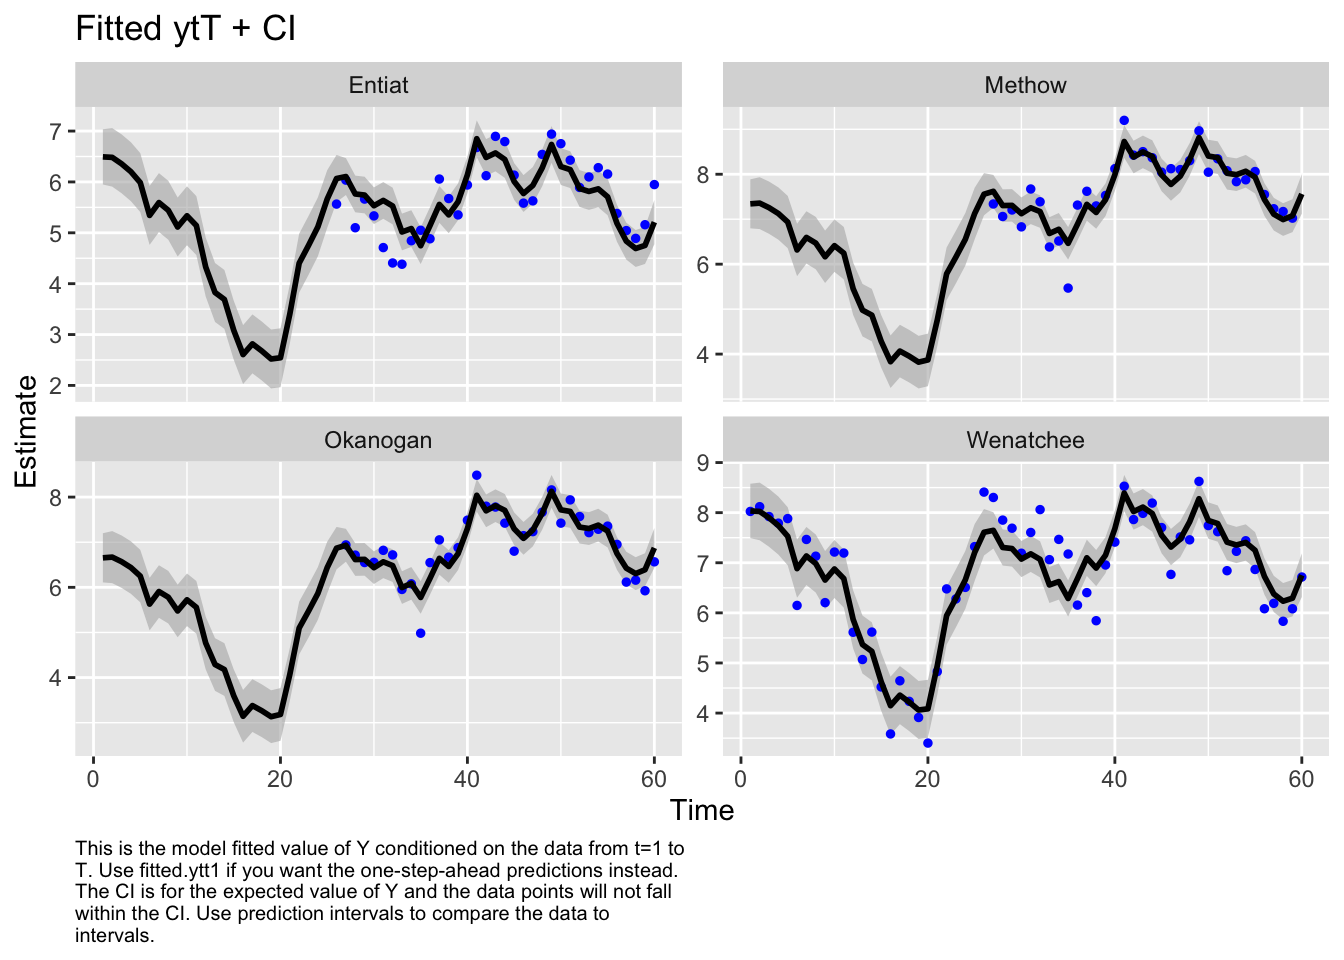
\includegraphics{Lab-1-Emma-ZR-MHS-draft_files/figure-latex/unnamed-chunk-22-1.pdf}

\begin{Shaded}
\begin{Highlighting}[]
\CommentTok{\#PACF plots for each region}
\FunctionTok{par}\NormalTok{(}\AttributeTok{mfrow=}\FunctionTok{c}\NormalTok{(}\DecValTok{3}\NormalTok{,}\DecValTok{4}\NormalTok{))}
\ControlFlowTok{for}\NormalTok{(r }\ControlFlowTok{in} \DecValTok{1}\SpecialCharTok{:}\FunctionTok{length}\NormalTok{(regions))\{}
  \FunctionTok{plot}\NormalTok{(DiagPlots[[r]][[}\DecValTok{2}\NormalTok{]], }\AttributeTok{main =} \FunctionTok{paste0}\NormalTok{(}\StringTok{"Region: "}\NormalTok{, regionskey[r]))}
\NormalTok{\}}
\end{Highlighting}
\end{Shaded}

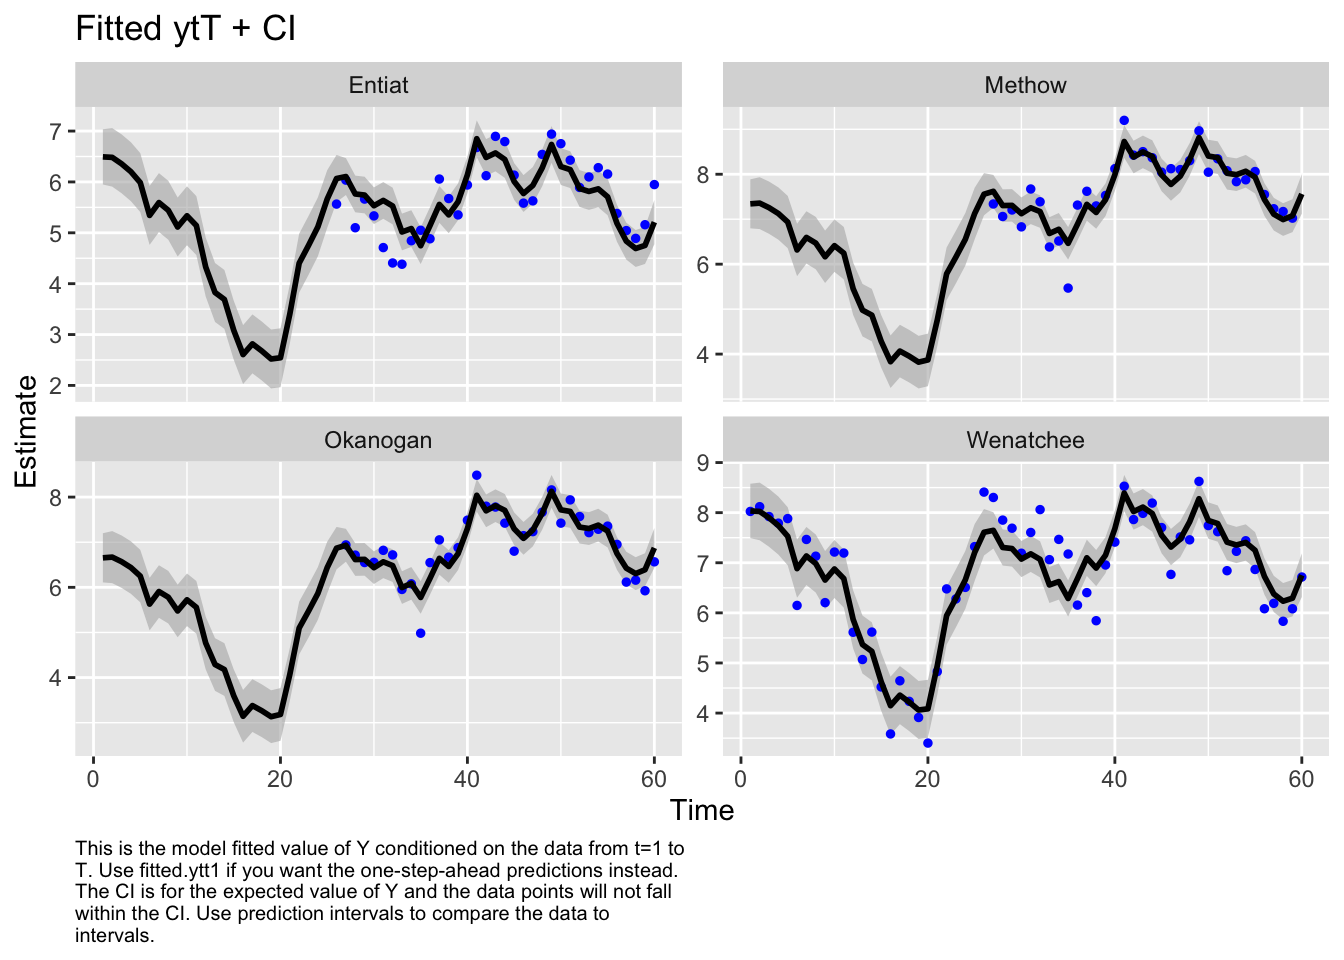
\includegraphics{Lab-1-Emma-ZR-MHS-draft_files/figure-latex/unnamed-chunk-22-2.pdf}

\begin{Shaded}
\begin{Highlighting}[]
\CommentTok{\#function for ARIMA models}
\NormalTok{FitModFunction}\OtherTok{\textless{}{-}}\ControlFlowTok{function}\NormalTok{(reg, forelevel)\{}
  \CommentTok{\#This function takes a region and forecast level, subsets the data according to these parameters, then sets up the time series object, and the test and train sets. It uses auto.arima to find the "best" model and then this is checked by comparing other models with DeltaAICc \textless{} 2 and the number of parameters. If auto.arima picked a the model with the lowest AIC and the fewest parameters, it forecasts using this model and checks forecast accuracy with MASE. If not, it refits the model using Arima and the simpler model, and then checks forecast accuracy with this.}
  \CommentTok{\#filter region}
\NormalTok{  Chumdat}\OtherTok{\textless{}{-}}\NormalTok{ChumByRegion }\SpecialCharTok{\%\textgreater{}\%} \FunctionTok{filter}\NormalTok{(region }\SpecialCharTok{==}\NormalTok{ reg)}
  \CommentTok{\#create time series}
\NormalTok{  datts }\OtherTok{\textless{}{-}} \FunctionTok{ts}\NormalTok{(Chumdat}\SpecialCharTok{$}\NormalTok{lnreturns, }\AttributeTok{start=}\NormalTok{Chumdat}\SpecialCharTok{$}\NormalTok{year[}\DecValTok{1}\NormalTok{]) }\CommentTok{\#this assumes the first year in data is the start of the time series (they are in order) }
\NormalTok{  cutoff}\OtherTok{\textless{}{-}}\DecValTok{2015}\SpecialCharTok{{-}}\NormalTok{forelevel}
\NormalTok{  train }\OtherTok{\textless{}{-}} \FunctionTok{window}\NormalTok{(datts, }\DecValTok{1952}\NormalTok{, cutoff)}
\NormalTok{  test }\OtherTok{\textless{}{-}} \FunctionTok{window}\NormalTok{(datts, cutoff}\SpecialCharTok{+}\DecValTok{1}\NormalTok{, }\DecValTok{2015}\NormalTok{)}
  
\NormalTok{  mod }\OtherTok{\textless{}{-}} \FunctionTok{auto.arima}\NormalTok{(train)}
  
  \CommentTok{\#testing to be sure that this is the best model (is the best mode the simplest if it is within 2 AIC values?)}
\NormalTok{  trace }\OtherTok{\textless{}{-}} \FunctionTok{capture.output}\NormalTok{(\{}
    \CommentTok{\# assign so it doesn\textquotesingle{}t pollute the output}
\NormalTok{    model }\OtherTok{\textless{}{-}} \FunctionTok{auto.arima}\NormalTok{(datts, }\AttributeTok{trace =} \ConstantTok{TRUE}\NormalTok{)}
\NormalTok{  \})}
\NormalTok{  con    }\OtherTok{\textless{}{-}} \FunctionTok{textConnection}\NormalTok{(trace)}
\NormalTok{  models }\OtherTok{\textless{}{-}} \FunctionTok{read.table}\NormalTok{(con, }\AttributeTok{sep=}\StringTok{":"}\NormalTok{)}
  \FunctionTok{close}\NormalTok{(con)}
  
  \CommentTok{\#getting the "best models" that are within 2 AIC units}
\NormalTok{  BestMods}\OtherTok{\textless{}{-}}\NormalTok{models}\SpecialCharTok{\%\textgreater{}\%} \FunctionTok{filter}\NormalTok{(}\FunctionTok{row\_number}\NormalTok{() }\SpecialCharTok{!=} \FunctionTok{nrow}\NormalTok{(models)) }\SpecialCharTok{\%\textgreater{}\%} \FunctionTok{mutate}\NormalTok{(}\AttributeTok{AIC =} \FunctionTok{replace}\NormalTok{(V2, V2 }\SpecialCharTok{==} \StringTok{"Inf"}\NormalTok{, }\DecValTok{99999}\NormalTok{), }\AttributeTok{AIC =} \FunctionTok{as.numeric}\NormalTok{(AIC), }\AttributeTok{DeltaAIC =}\NormalTok{ AIC}\SpecialCharTok{{-}}\FunctionTok{min}\NormalTok{(AIC)) }\SpecialCharTok{\%\textgreater{}\%} \FunctionTok{filter}\NormalTok{(DeltaAIC }\SpecialCharTok{\textless{}=} \FloatTok{2.0}\NormalTok{)}
  \ControlFlowTok{for}\NormalTok{(i }\ControlFlowTok{in} \DecValTok{1}\SpecialCharTok{:}\FunctionTok{nrow}\NormalTok{(BestMods))\{}
\NormalTok{    BestMods}\SpecialCharTok{$}\NormalTok{Mod[i]}\OtherTok{\textless{}{-}}\FunctionTok{strsplit}\NormalTok{(}\FunctionTok{strsplit}\NormalTok{(}\FunctionTok{strsplit}\NormalTok{(BestMods}\SpecialCharTok{$}\NormalTok{V1[i], }\StringTok{"[(]"}\NormalTok{)[[}\DecValTok{1}\NormalTok{]][}\DecValTok{2}\NormalTok{], }\StringTok{"[)]"}\NormalTok{)[[}\DecValTok{1}\NormalTok{]][}\DecValTok{1}\NormalTok{],}\StringTok{"[,]"}\NormalTok{)}
\NormalTok{    BestMods}\SpecialCharTok{$}\NormalTok{npar[i]}\OtherTok{\textless{}{-}}\FunctionTok{sum}\NormalTok{(}\FunctionTok{as.numeric}\NormalTok{(BestMods}\SpecialCharTok{$}\NormalTok{Mod[i][[}\DecValTok{1}\NormalTok{]][}\FunctionTok{c}\NormalTok{(}\DecValTok{1}\NormalTok{,}\DecValTok{3}\NormalTok{)]))}
    \ControlFlowTok{if}\NormalTok{(}\FunctionTok{strsplit}\NormalTok{(}\FunctionTok{strsplit}\NormalTok{(BestMods}\SpecialCharTok{$}\NormalTok{V1[i], }\StringTok{"[(]"}\NormalTok{)[[}\DecValTok{1}\NormalTok{]][}\DecValTok{2}\NormalTok{], }\StringTok{"[)]"}\NormalTok{)[[}\DecValTok{1}\NormalTok{]][}\DecValTok{2}\NormalTok{] }\SpecialCharTok{==} \StringTok{" with drift         "}\NormalTok{)\{}
\NormalTok{      BestMods}\SpecialCharTok{$}\NormalTok{npar[i] }\OtherTok{=}\NormalTok{ BestMods}\SpecialCharTok{$}\NormalTok{npar[i] }\SpecialCharTok{+} \DecValTok{1}
\NormalTok{    \}}
\NormalTok{  \}}
  
\NormalTok{  New}\OtherTok{\textless{}{-}}\NormalTok{BestMods }\SpecialCharTok{\%\textgreater{}\%} \FunctionTok{filter}\NormalTok{(npar }\SpecialCharTok{==} \FunctionTok{min}\NormalTok{(npar))}
  \ControlFlowTok{if}\NormalTok{(}\DecValTok{0} \SpecialCharTok{\%in\%}\NormalTok{ New}\SpecialCharTok{$}\NormalTok{DeltaAIC)\{}
      \CommentTok{\#auto arima picked the best model}
\NormalTok{      res}\OtherTok{\textless{}{-}}\FunctionTok{accuracy}\NormalTok{(}\FunctionTok{forecast}\NormalTok{(mod, }\AttributeTok{h=}\NormalTok{forelevel), test)[}\DecValTok{2}\NormalTok{,}\StringTok{"MASE"}\NormalTok{] }\CommentTok{\#test set MASE}
\NormalTok{  \}}\ControlFlowTok{else}\NormalTok{\{}
      \CommentTok{\#of the models with the fewest parameters, pick the lowest AIC}
\NormalTok{      newmod}\OtherTok{\textless{}{-}}\NormalTok{New }\SpecialCharTok{\%\textgreater{}\%} \FunctionTok{filter}\NormalTok{(AIC }\SpecialCharTok{==} \FunctionTok{min}\NormalTok{(AIC)) }\SpecialCharTok{\%\textgreater{}\%} \FunctionTok{select}\NormalTok{(Mod)}
\NormalTok{      mod}\OtherTok{\textless{}{-}}\FunctionTok{Arima}\NormalTok{(train, }\AttributeTok{order =} \FunctionTok{as.numeric}\NormalTok{(}\FunctionTok{strsplit}\NormalTok{(newmod}\SpecialCharTok{$}\NormalTok{Mod[[}\DecValTok{1}\NormalTok{]], }\StringTok{"[,]"}\NormalTok{)), }\AttributeTok{include.constant =} \ConstantTok{TRUE}\NormalTok{)}
\NormalTok{      res}\OtherTok{\textless{}{-}}\FunctionTok{accuracy}\NormalTok{(}\FunctionTok{forecast}\NormalTok{(mod, }\AttributeTok{h=}\NormalTok{forelevel), test)[}\DecValTok{2}\NormalTok{,}\StringTok{"MASE"}\NormalTok{] }\CommentTok{\#test set MASE}
\NormalTok{    \}}

  \FunctionTok{return}\NormalTok{(}\FunctionTok{list}\NormalTok{(}\AttributeTok{Fit =}\NormalTok{ mod, }\AttributeTok{MASE =}\NormalTok{ res, }\AttributeTok{Bm =}\NormalTok{ BestMods)) }\CommentTok{\#include best mods for testing to see that it\textquotesingle{}s doing what I want}
\NormalTok{\}}
\end{Highlighting}
\end{Shaded}

\begin{Shaded}
\begin{Highlighting}[]
\NormalTok{RegionModsChum}\OtherTok{\textless{}{-}}\FunctionTok{mapply}\NormalTok{(FitModFunction, Allcombs}\SpecialCharTok{$}\NormalTok{regions, Allcombs}\SpecialCharTok{$}\NormalTok{forecastlevels, }\AttributeTok{SIMPLIFY =} \ConstantTok{FALSE}\NormalTok{)}
\end{Highlighting}
\end{Shaded}

\begin{Shaded}
\begin{Highlighting}[]
\NormalTok{RegionMASEChum}\OtherTok{\textless{}{-}}\FunctionTok{sapply}\NormalTok{(RegionModsChum, }\ControlFlowTok{function}\NormalTok{(x)\{y}\OtherTok{\textless{}{-}}\NormalTok{x}\SpecialCharTok{$}\NormalTok{MASE\})}
\NormalTok{RegionBestModChum}\OtherTok{\textless{}{-}}\FunctionTok{sapply}\NormalTok{(RegionModsChum, }\ControlFlowTok{function}\NormalTok{(x)\{y}\OtherTok{\textless{}{-}}\FunctionTok{as.character}\NormalTok{(x}\SpecialCharTok{$}\NormalTok{Fit)\})}
\CommentTok{\#combine into tables}
\NormalTok{ResultsTableChum}\OtherTok{\textless{}{-}}\NormalTok{Allcombs }\SpecialCharTok{\%\textgreater{}\%} \FunctionTok{add\_column}\NormalTok{(}\AttributeTok{Model =}\NormalTok{ RegionBestModChum, }\AttributeTok{MASE =}\NormalTok{ RegionMASEChum)}
\NormalTok{knitr}\SpecialCharTok{::}\FunctionTok{kable}\NormalTok{(}\FunctionTok{head}\NormalTok{(ResultsTableChum))}
\end{Highlighting}
\end{Shaded}

\begin{longtable}[]{@{}lrlr@{}}
\toprule()
regions & forecastlevels & Model & MASE \\
\midrule()
\endhead
ci & 5 & ARIMA(1,1,1) & 0.4232248 \\
ci & 10 & ARIMA(1,1,1) & 0.3650863 \\
ci & 20 & ARIMA(0,0,2) with non-zero mean & 1.3678453 \\
e\_kam & 5 & ARIMA(1,0,0) with non-zero mean & 2.0352335 \\
e\_kam & 10 & ARIMA(1,0,0) with non-zero mean & 1.6504750 \\
e\_kam & 20 & ARIMA(1,0,0) with non-zero mean & 1.4845904 \\
\bottomrule()
\end{longtable}

\hypertarget{pink-combined-regions}{%
\subsection{Pink: Combined Regions}\label{pink-combined-regions}}

Subset the data to look at pink salmon only.

\begin{Shaded}
\begin{Highlighting}[]
\CommentTok{\#Filter by species (Pink)}
\NormalTok{dat }\OtherTok{\textless{}{-}}\NormalTok{ ruggerone\_data }\SpecialCharTok{\%\textgreater{}\%}  
  \FunctionTok{filter}\NormalTok{(species}\SpecialCharTok{==}\StringTok{"pink"} \SpecialCharTok{\&}\NormalTok{ region}\SpecialCharTok{==}\StringTok{"ci"}\NormalTok{) }\SpecialCharTok{\%\textgreater{}\%} 
  \FunctionTok{mutate}\NormalTok{(}\AttributeTok{log.returns =} \FunctionTok{log}\NormalTok{(returns)) }\SpecialCharTok{\%\textgreater{}\%} 
  \FunctionTok{select}\NormalTok{(year, log.returns)}
\end{Highlighting}
\end{Shaded}

Plot the data

\begin{Shaded}
\begin{Highlighting}[]
\CommentTok{\#Plot by region}
\NormalTok{ruggerone\_data }\SpecialCharTok{\%\textgreater{}\%} 
  \FunctionTok{filter}\NormalTok{(species}\SpecialCharTok{==}\StringTok{"pink"}\NormalTok{) }\SpecialCharTok{\%\textgreater{}\%} 
  \FunctionTok{ggplot}\NormalTok{(}\FunctionTok{aes}\NormalTok{(}\AttributeTok{x=}\NormalTok{year, }\AttributeTok{y=}\FunctionTok{log}\NormalTok{(returns))) }\SpecialCharTok{+} 
  \FunctionTok{geom\_line}\NormalTok{() }\SpecialCharTok{+} 
  \FunctionTok{ggtitle}\NormalTok{(}\StringTok{"pink salmon log abundance by region"}\NormalTok{) }\SpecialCharTok{+}
  \FunctionTok{facet\_wrap}\NormalTok{(}\SpecialCharTok{\textasciitilde{}}\NormalTok{region)}
\end{Highlighting}
\end{Shaded}

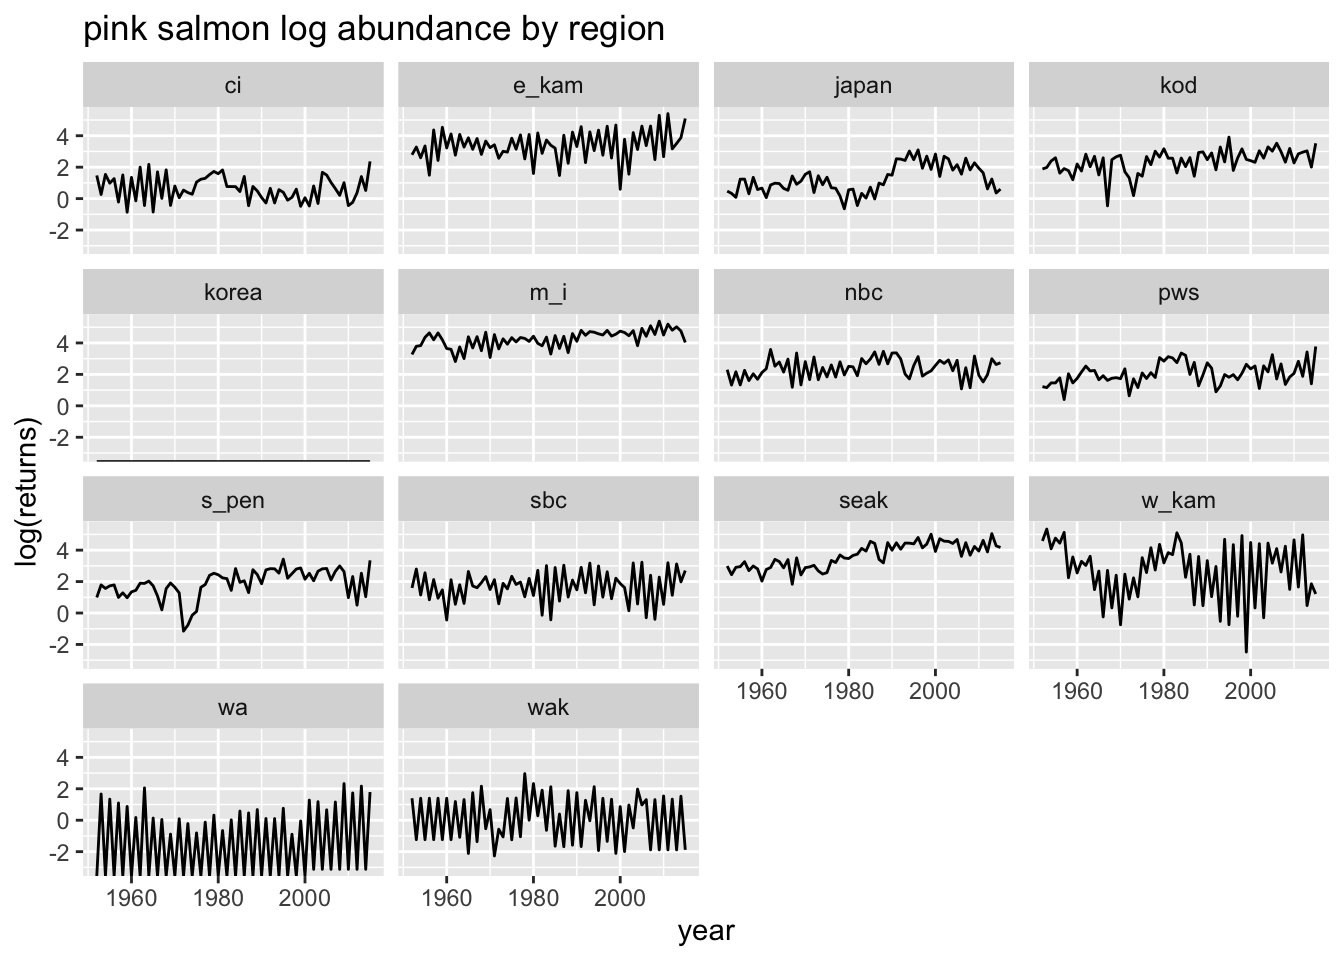
\includegraphics{Lab-1-Emma-ZR-MHS-draft_files/figure-latex/unnamed-chunk-27-1.pdf}

Note that there is no data in Korea, and WA has a lot of 0 values and
very low returns. We will filter these regions out. All 0 values (-Inf
in log space) were removed.

\begin{Shaded}
\begin{Highlighting}[]
\NormalTok{PinkByRegion}\OtherTok{\textless{}{-}}\NormalTok{ruggerone\_data }\SpecialCharTok{\%\textgreater{}\%}
  \FunctionTok{filter}\NormalTok{(region }\SpecialCharTok{!=} \StringTok{"korea"}\NormalTok{) }\SpecialCharTok{\%\textgreater{}\%} 
  \FunctionTok{filter}\NormalTok{(region }\SpecialCharTok{!=} \StringTok{"wa"}\NormalTok{) }\SpecialCharTok{\%\textgreater{}\%}\CommentTok{\#Remove WA too, it\textquotesingle{}s trouble }
  \FunctionTok{group\_by}\NormalTok{(species, region, year) }\SpecialCharTok{\%\textgreater{}\%}
  \FunctionTok{summarize}\NormalTok{(}\AttributeTok{total =} \FunctionTok{sum}\NormalTok{(returns, }\AttributeTok{na.rm=}\ConstantTok{TRUE}\NormalTok{)) }\SpecialCharTok{\%\textgreater{}\%} 
  \FunctionTok{mutate}\NormalTok{(}\AttributeTok{lnreturns =} \FunctionTok{log}\NormalTok{(total)) }\SpecialCharTok{\%\textgreater{}\%}
  \FunctionTok{mutate}\NormalTok{(}\AttributeTok{lnreturns =} \FunctionTok{ifelse}\NormalTok{(lnreturns }\SpecialCharTok{==} \SpecialCharTok{{-}}\ConstantTok{Inf}\NormalTok{, }\ConstantTok{NA}\NormalTok{, lnreturns)) }\SpecialCharTok{\%\textgreater{}\%}
  \FunctionTok{filter}\NormalTok{(species }\SpecialCharTok{==} \StringTok{"pink"}\NormalTok{)}\SpecialCharTok{\%\textgreater{}\%} 
  \FunctionTok{print}\NormalTok{(}\AttributeTok{n=}\DecValTok{5}\NormalTok{)}
\end{Highlighting}
\end{Shaded}

\begin{verbatim}
## `summarise()` has grouped output by 'species', 'region'. You can override using
## the `.groups` argument.
\end{verbatim}

\begin{verbatim}
## # A tibble: 768 x 5
## # Groups:   species, region [12]
##   species region  year total lnreturns
##   <chr>   <chr>  <dbl> <dbl>     <dbl>
## 1 pink    ci      1952  4.36     1.47 
## 2 pink    ci      1953  1.30     0.264
## 3 pink    ci      1954  4.67     1.54 
## 4 pink    ci      1955  2.67     0.981
## 5 pink    ci      1956  3.57     1.27 
## # i 763 more rows
\end{verbatim}

Identify start and end years for each region.

\begin{Shaded}
\begin{Highlighting}[]
\NormalTok{PinkByRegion }\SpecialCharTok{\%\textgreater{}\%} \FunctionTok{group\_by}\NormalTok{(region) }\SpecialCharTok{\%\textgreater{}\%} \FunctionTok{summarise}\NormalTok{(}\AttributeTok{startyear =} \FunctionTok{min}\NormalTok{(year), }\AttributeTok{endyear =} \FunctionTok{max}\NormalTok{(year))}
\end{Highlighting}
\end{Shaded}

\begin{verbatim}
## # A tibble: 12 x 3
##    region startyear endyear
##    <chr>      <dbl>   <dbl>
##  1 ci          1952    2015
##  2 e_kam       1952    2015
##  3 japan       1952    2015
##  4 kod         1952    2015
##  5 m_i         1952    2015
##  6 nbc         1952    2015
##  7 pws         1952    2015
##  8 s_pen       1952    2015
##  9 sbc         1952    2015
## 10 seak        1952    2015
## 11 w_kam       1952    2015
## 12 wak         1952    2015
\end{verbatim}

The next step is to ID Stationarity with all the pink data. Lets plot
the data in aggregate.

\begin{Shaded}
\begin{Highlighting}[]
\NormalTok{PinkByRegion }\SpecialCharTok{\%\textgreater{}\%}
  \FunctionTok{group\_by}\NormalTok{(year) }\SpecialCharTok{\%\textgreater{}\%}
  \FunctionTok{summarize}\NormalTok{(}\AttributeTok{total =} \FunctionTok{sum}\NormalTok{(total, }\AttributeTok{na.rm=}\NormalTok{T)) }\SpecialCharTok{\%\textgreater{}\%}
  \FunctionTok{ggplot}\NormalTok{(}\FunctionTok{aes}\NormalTok{(}\AttributeTok{x=}\NormalTok{year, }\AttributeTok{y=}\FunctionTok{log}\NormalTok{(total))) }\SpecialCharTok{+}
  \FunctionTok{geom\_line}\NormalTok{() }\SpecialCharTok{+}
  \FunctionTok{ylab}\NormalTok{(}\StringTok{\textquotesingle{}Log (Returns)\textquotesingle{}}\NormalTok{) }\SpecialCharTok{+}
  \FunctionTok{xlab}\NormalTok{(}\StringTok{\textquotesingle{}Year\textquotesingle{}}\NormalTok{)}
\end{Highlighting}
\end{Shaded}

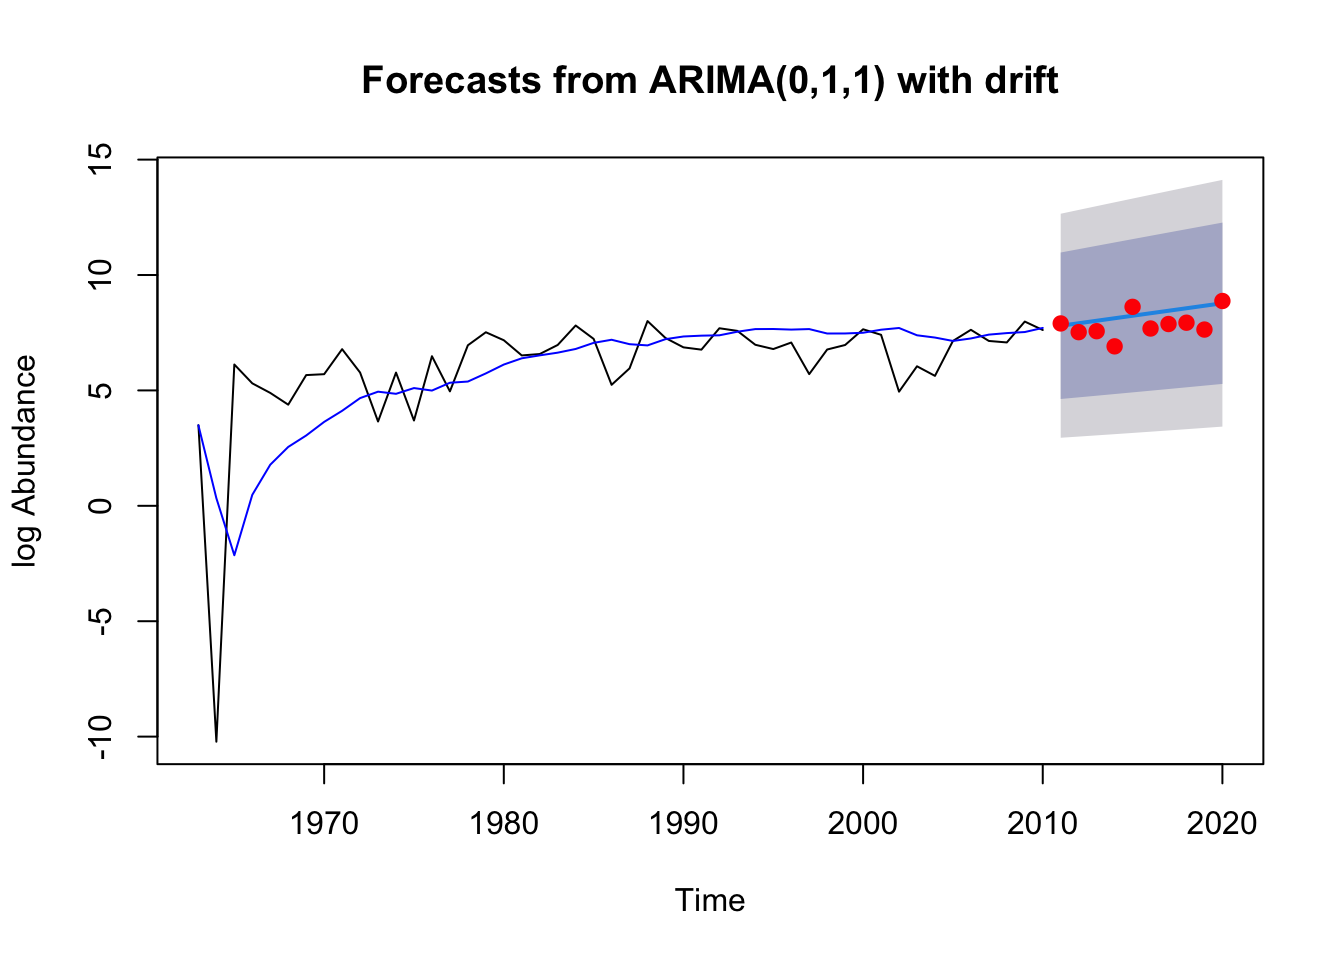
\includegraphics{Lab-1-Emma-ZR-MHS-draft_files/figure-latex/unnamed-chunk-30-1.pdf}

Next, a time series object was created and we look at the ACF and PACF

\begin{Shaded}
\begin{Highlighting}[]
\NormalTok{total.pink}\OtherTok{\textless{}{-}}\NormalTok{PinkByRegion }\SpecialCharTok{\%\textgreater{}\%}
  \FunctionTok{group\_by}\NormalTok{(year) }\SpecialCharTok{\%\textgreater{}\%}
  \FunctionTok{summarize}\NormalTok{(}\AttributeTok{lntotal=}\FunctionTok{log}\NormalTok{(}\FunctionTok{sum}\NormalTok{(total, }\AttributeTok{na.rm=}\NormalTok{T)))}

\NormalTok{pink.ts}\OtherTok{\textless{}{-}}\FunctionTok{ts}\NormalTok{(total.pink}\SpecialCharTok{$}\NormalTok{lntotal, }
            \AttributeTok{start=}\NormalTok{total.pink}\SpecialCharTok{$}\NormalTok{year[}\DecValTok{1}\NormalTok{])}
\FunctionTok{plot}\NormalTok{(}\FunctionTok{diff}\NormalTok{(pink.ts)) }\CommentTok{\#something odd happened between 1990 and 2005}
\end{Highlighting}
\end{Shaded}

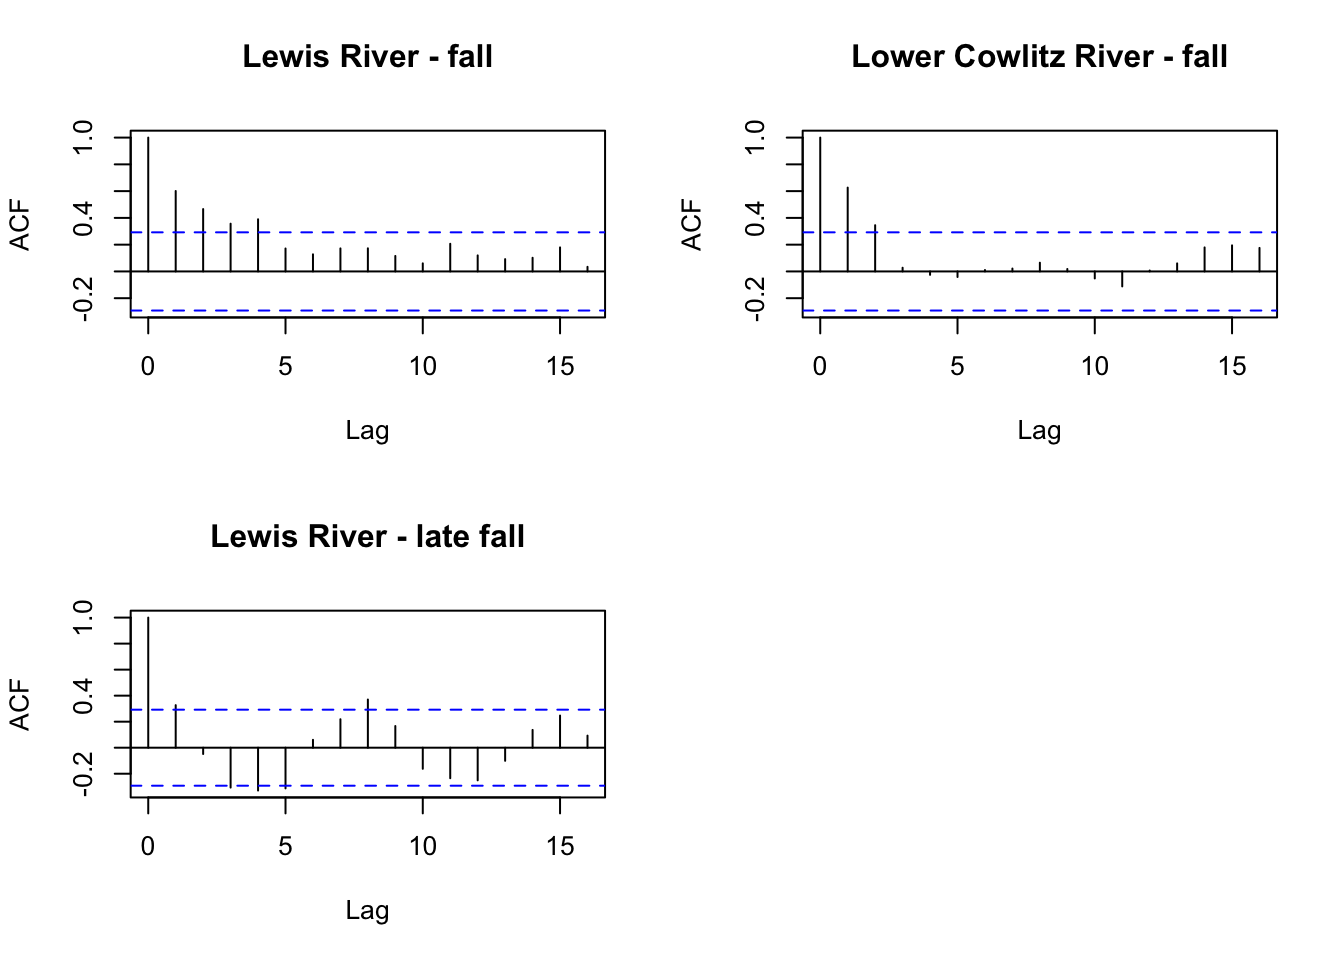
\includegraphics{Lab-1-Emma-ZR-MHS-draft_files/figure-latex/unnamed-chunk-31-1.pdf}

\begin{Shaded}
\begin{Highlighting}[]
\FunctionTok{acf}\NormalTok{(}\FunctionTok{diff}\NormalTok{(pink.ts)) }\CommentTok{\#ruh roh, ACF correlation for entire series }
\end{Highlighting}
\end{Shaded}

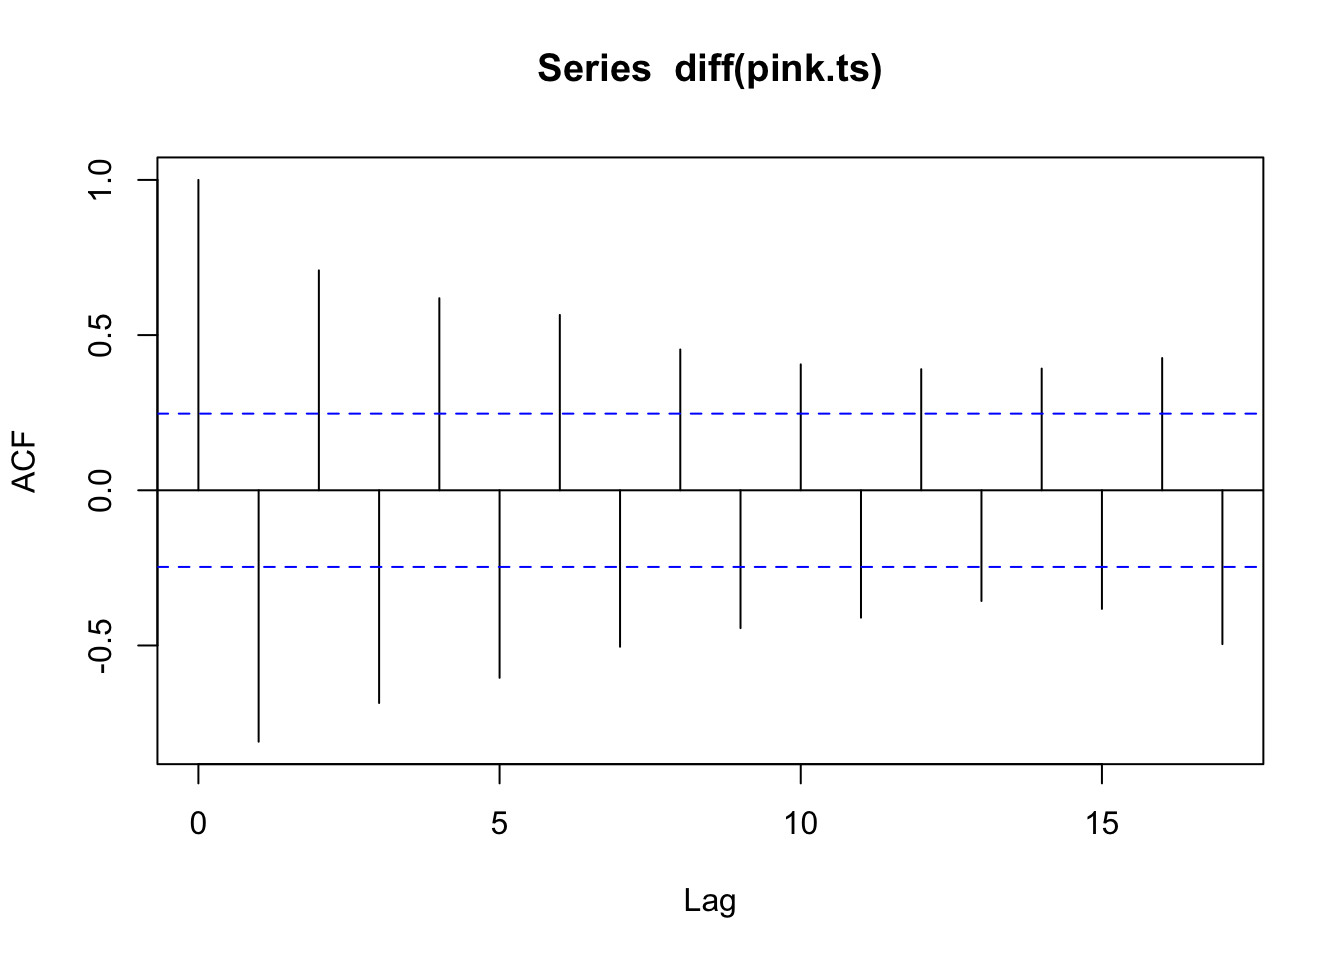
\includegraphics{Lab-1-Emma-ZR-MHS-draft_files/figure-latex/unnamed-chunk-31-2.pdf}
The ACF looks like there is a lot of corelation, that's probably because
Pinks have a very consistent two year cycle.

Let's try a forecast model to see what happens.

\begin{Shaded}
\begin{Highlighting}[]
\CommentTok{\#Let\textquotesingle{}s train and test with a 10 year period}
\NormalTok{train.pink}\OtherTok{\textless{}{-}}\FunctionTok{window}\NormalTok{(pink.ts, }\AttributeTok{start=}\DecValTok{1952}\NormalTok{, }\AttributeTok{end=}\DecValTok{2005}\NormalTok{)}
\NormalTok{test.pink}\OtherTok{\textless{}{-}}\FunctionTok{window}\NormalTok{(pink.ts, }\AttributeTok{start=}\DecValTok{2006}\NormalTok{, }\AttributeTok{end=}\DecValTok{2015}\NormalTok{)}

\NormalTok{fit }\OtherTok{\textless{}{-}}\NormalTok{ forecast}\SpecialCharTok{::}\FunctionTok{auto.arima}\NormalTok{(train.pink, }\AttributeTok{trace=}\NormalTok{T)}
\end{Highlighting}
\end{Shaded}

\begin{verbatim}
## 
##  ARIMA(2,1,2) with drift         : Inf
##  ARIMA(0,1,0) with drift         : 44.48651
##  ARIMA(1,1,0) with drift         : -0.8966894
##  ARIMA(0,1,1) with drift         : 18.15923
##  ARIMA(0,1,0)                    : 42.45004
##  ARIMA(2,1,0) with drift         : -1.222687
##  ARIMA(3,1,0) with drift         : -2.155628
##  ARIMA(4,1,0) with drift         : 0.3831016
##  ARIMA(3,1,1) with drift         : 0.2902468
##  ARIMA(2,1,1) with drift         : Inf
##  ARIMA(4,1,1) with drift         : Inf
##  ARIMA(3,1,0)                    : -4.270823
##  ARIMA(2,1,0)                    : -3.360303
##  ARIMA(4,1,0)                    : -1.841485
##  ARIMA(3,1,1)                    : -1.889482
##  ARIMA(2,1,1)                    : Inf
##  ARIMA(4,1,1)                    : 0.4019518
## 
##  Best model: ARIMA(3,1,0)
\end{verbatim}

\begin{Shaded}
\begin{Highlighting}[]
\NormalTok{fit.final.pink}\OtherTok{\textless{}{-}}\NormalTok{forecast}\SpecialCharTok{::}\FunctionTok{auto.arima}\NormalTok{(train.pink, }\AttributeTok{approximation =}\NormalTok{ F, }\AttributeTok{stepwise =}\NormalTok{ F)}

\CommentTok{\#30 year forcast, not so believeable}
\NormalTok{fit.final.pink }\SpecialCharTok{\%\textgreater{}\%}
  \FunctionTok{forecast}\NormalTok{(}\AttributeTok{h=}\DecValTok{15}\NormalTok{) }\SpecialCharTok{\%\textgreater{}\%}
  \FunctionTok{autoplot}\NormalTok{() }\SpecialCharTok{+} \FunctionTok{geom\_point}\NormalTok{(}\FunctionTok{aes}\NormalTok{(}\AttributeTok{x=}\NormalTok{x, }\AttributeTok{y=}\NormalTok{y), }\AttributeTok{data=}\FunctionTok{fortify}\NormalTok{(test.pink))}
\end{Highlighting}
\end{Shaded}

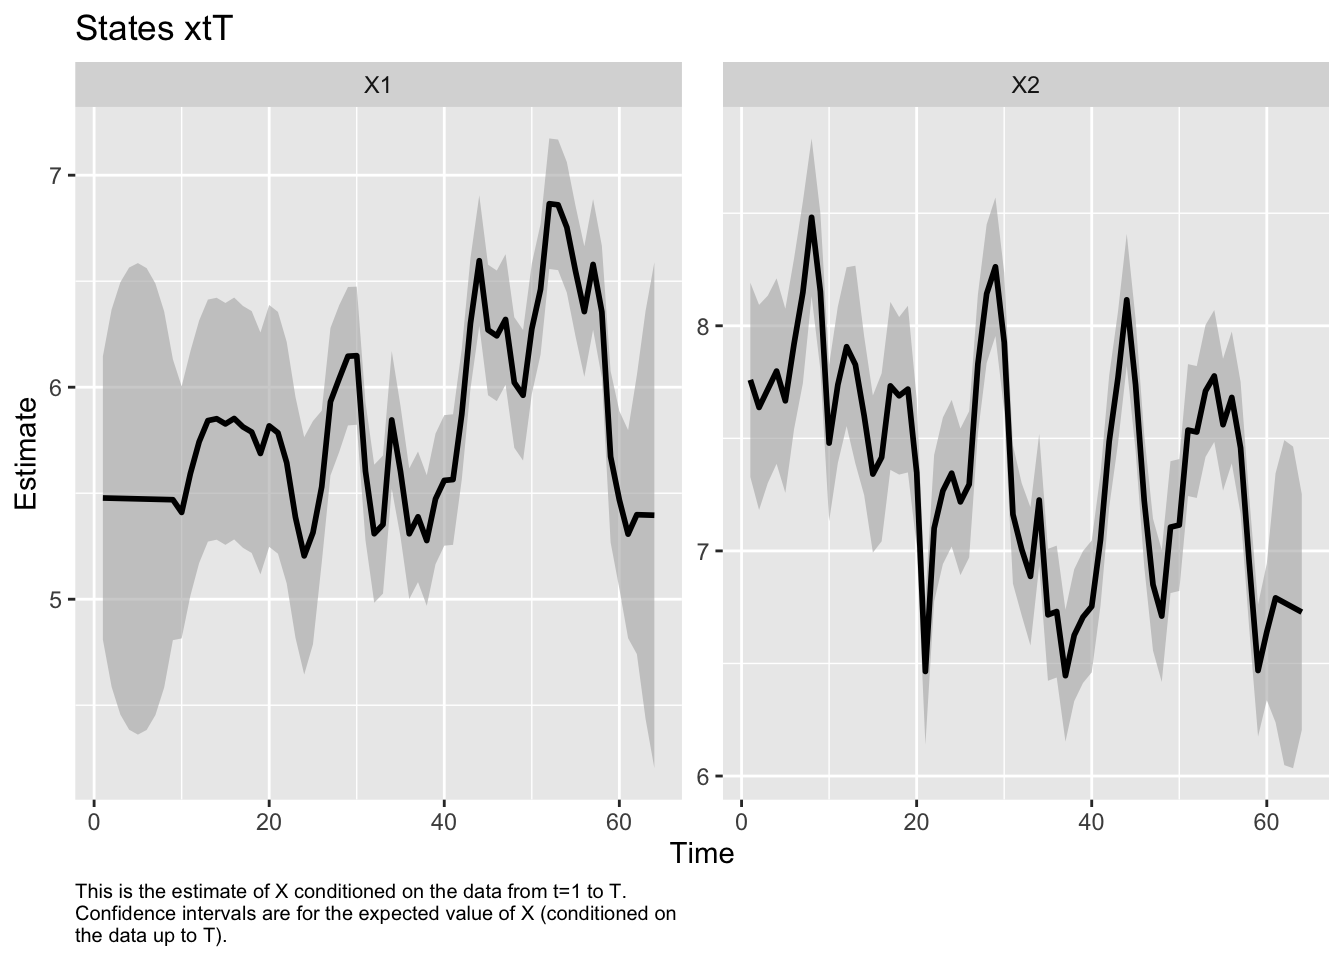
\includegraphics{Lab-1-Emma-ZR-MHS-draft_files/figure-latex/unnamed-chunk-32-1.pdf}

The best model was the ARIMA(3,1,0), but the forecast doesn't look
particularly great.

Given the life history of pink salmon, let's parse the data set into two
pieces, even and odd years.

\begin{Shaded}
\begin{Highlighting}[]
\CommentTok{\#Even Years: Totals }
\NormalTok{PinkByRegion\_even}\OtherTok{\textless{}{-}}\NormalTok{PinkByRegion }\SpecialCharTok{\%\textgreater{}\%} 
  \FunctionTok{filter}\NormalTok{(year }\SpecialCharTok{\%\%} \DecValTok{2} \SpecialCharTok{==} \DecValTok{0}\NormalTok{)}

\CommentTok{\#Odd Years: Totals }
\NormalTok{PinkByRegion\_odd}\OtherTok{\textless{}{-}}\NormalTok{PinkByRegion }\SpecialCharTok{\%\textgreater{}\%} 
  \FunctionTok{filter}\NormalTok{(year }\SpecialCharTok{\%\%} \DecValTok{2} \SpecialCharTok{==} \DecValTok{1}\NormalTok{)}

\CommentTok{\#Trends}
\NormalTok{PinkByRegion\_even }\SpecialCharTok{\%\textgreater{}\%}
  \FunctionTok{group\_by}\NormalTok{(year) }\SpecialCharTok{\%\textgreater{}\%}
  \FunctionTok{summarize}\NormalTok{(}\AttributeTok{total =} \FunctionTok{sum}\NormalTok{(total, }\AttributeTok{na.rm=}\NormalTok{T)) }\SpecialCharTok{\%\textgreater{}\%}
  \FunctionTok{ggplot}\NormalTok{(}\FunctionTok{aes}\NormalTok{(}\AttributeTok{x=}\NormalTok{year, }\AttributeTok{y=}\FunctionTok{log}\NormalTok{(total))) }\SpecialCharTok{+}
  \FunctionTok{geom\_line}\NormalTok{() }\SpecialCharTok{+}
  \FunctionTok{ylab}\NormalTok{(}\StringTok{\textquotesingle{}Log (Returns)\textquotesingle{}}\NormalTok{) }\SpecialCharTok{+}
  \FunctionTok{xlab}\NormalTok{(}\StringTok{\textquotesingle{}Year\textquotesingle{}}\NormalTok{) }\SpecialCharTok{+}
  \FunctionTok{ggtitle}\NormalTok{(}\StringTok{\textquotesingle{}Total Pinks (Even Years)\textquotesingle{}}\NormalTok{)}
\end{Highlighting}
\end{Shaded}

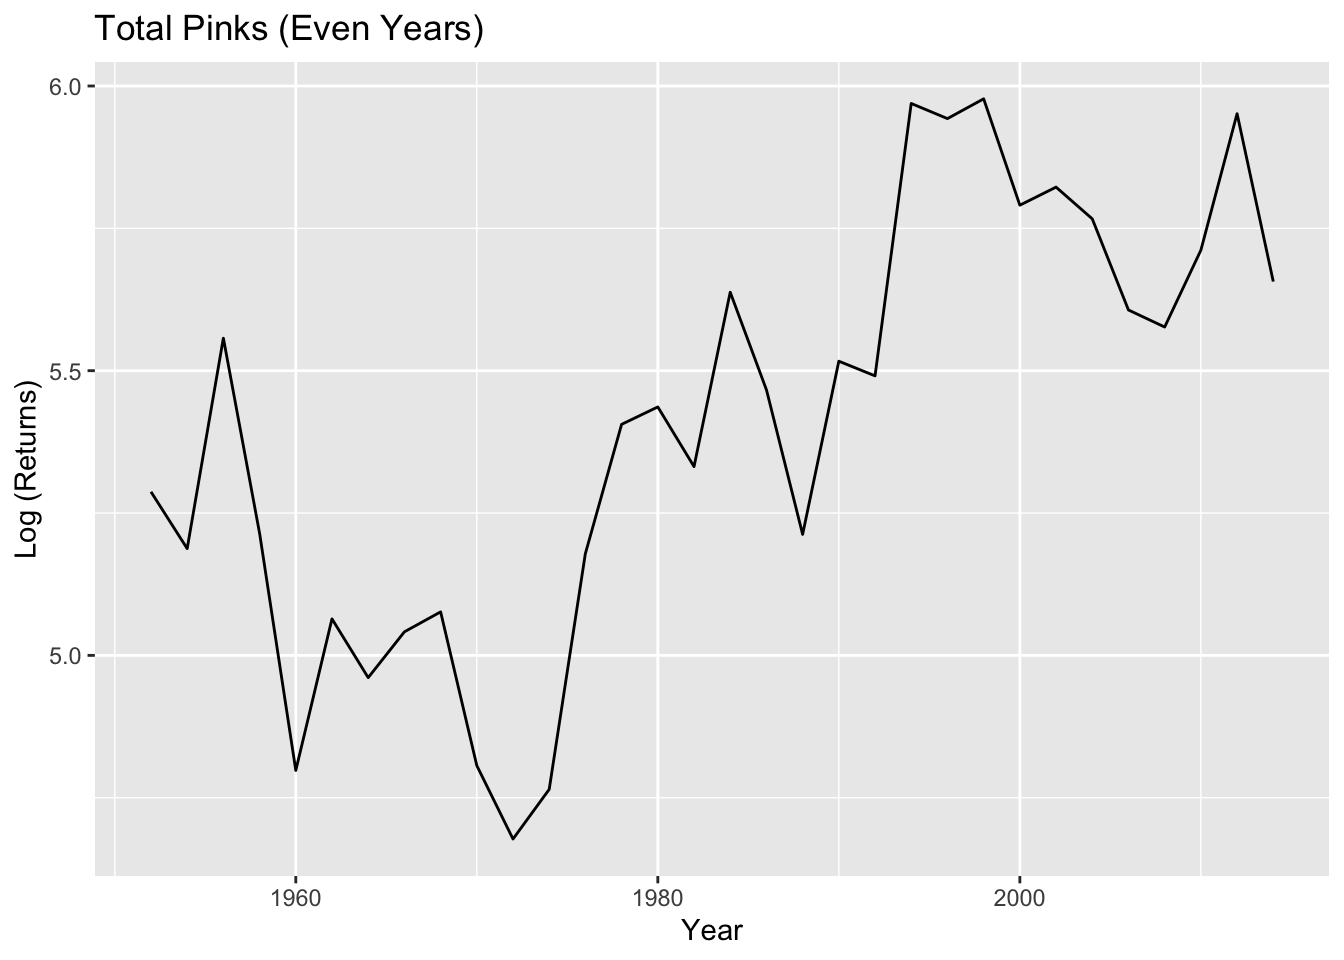
\includegraphics{Lab-1-Emma-ZR-MHS-draft_files/figure-latex/unnamed-chunk-33-1.pdf}

\begin{Shaded}
\begin{Highlighting}[]
\NormalTok{PinkByRegion\_odd }\SpecialCharTok{\%\textgreater{}\%}
  \FunctionTok{group\_by}\NormalTok{(year) }\SpecialCharTok{\%\textgreater{}\%}
  \FunctionTok{summarize}\NormalTok{(}\AttributeTok{total =} \FunctionTok{sum}\NormalTok{(total, }\AttributeTok{na.rm=}\NormalTok{T)) }\SpecialCharTok{\%\textgreater{}\%}
  \FunctionTok{ggplot}\NormalTok{(}\FunctionTok{aes}\NormalTok{(}\AttributeTok{x=}\NormalTok{year, }\AttributeTok{y=}\FunctionTok{log}\NormalTok{(total))) }\SpecialCharTok{+}
  \FunctionTok{geom\_line}\NormalTok{() }\SpecialCharTok{+}
  \FunctionTok{ylab}\NormalTok{(}\StringTok{\textquotesingle{}Log (Returns)\textquotesingle{}}\NormalTok{) }\SpecialCharTok{+}
  \FunctionTok{xlab}\NormalTok{(}\StringTok{\textquotesingle{}Year\textquotesingle{}}\NormalTok{) }\SpecialCharTok{+}
  \FunctionTok{ggtitle}\NormalTok{(}\StringTok{\textquotesingle{}Total Pinks (Odd Years)\textquotesingle{}}\NormalTok{)}
\end{Highlighting}
\end{Shaded}

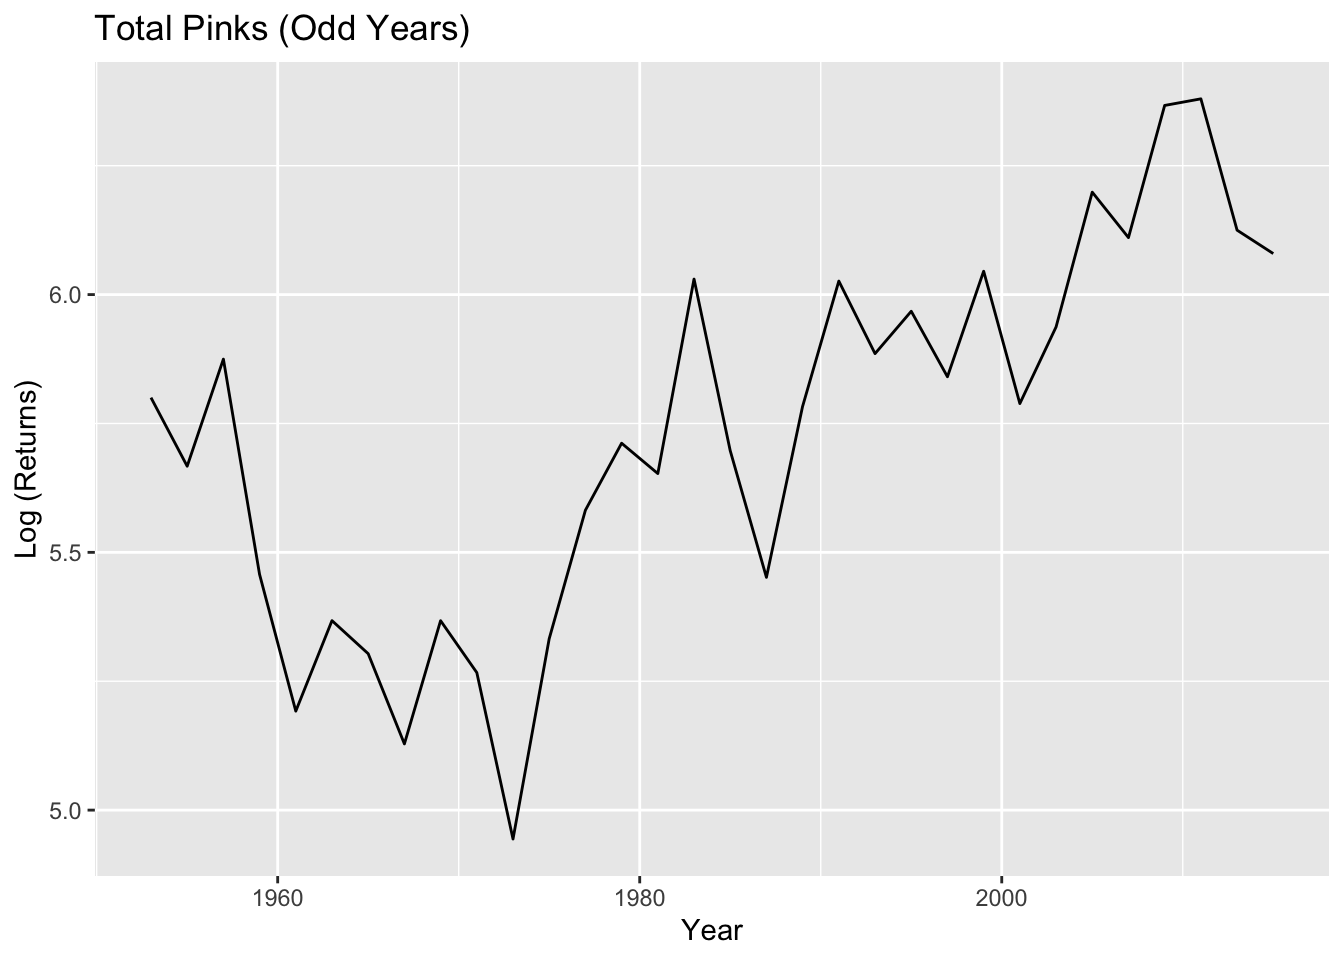
\includegraphics{Lab-1-Emma-ZR-MHS-draft_files/figure-latex/unnamed-chunk-33-2.pdf}

Let's look at the ACF and PACF for even years:

\begin{Shaded}
\begin{Highlighting}[]
\CommentTok{\#Even Years {-}{-} Total}
\NormalTok{total.pink\_even}\OtherTok{\textless{}{-}}\NormalTok{PinkByRegion\_even }\SpecialCharTok{\%\textgreater{}\%}
  \FunctionTok{group\_by}\NormalTok{(year) }\SpecialCharTok{\%\textgreater{}\%}
  \FunctionTok{summarize}\NormalTok{(}\AttributeTok{lntotal=}\FunctionTok{log}\NormalTok{(}\FunctionTok{sum}\NormalTok{(total, }\AttributeTok{na.rm=}\NormalTok{T)))}

\NormalTok{pink.ts\_even}\OtherTok{\textless{}{-}}\FunctionTok{ts}\NormalTok{(total.pink\_even}\SpecialCharTok{$}\NormalTok{lntotal, }
            \AttributeTok{start=}\NormalTok{total.pink}\SpecialCharTok{$}\NormalTok{year[}\DecValTok{1}\NormalTok{], }\AttributeTok{frequency =} \FloatTok{0.5}\NormalTok{)}
\FunctionTok{plot}\NormalTok{(}\FunctionTok{diff}\NormalTok{(pink.ts\_even)) }\CommentTok{\#Looks pretty stationary}
\end{Highlighting}
\end{Shaded}

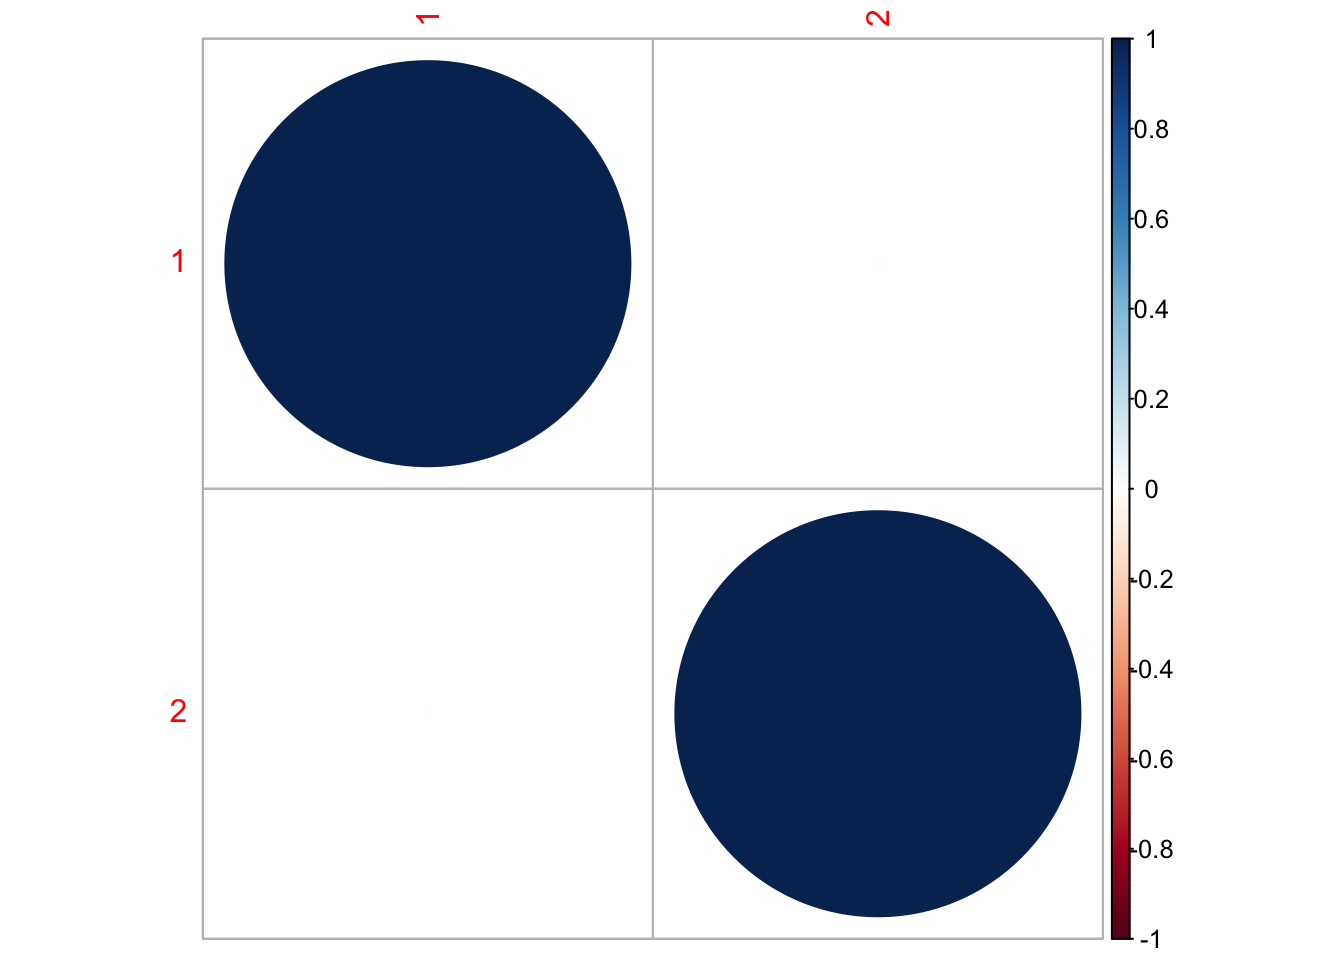
\includegraphics{Lab-1-Emma-ZR-MHS-draft_files/figure-latex/unnamed-chunk-34-1.pdf}

\begin{Shaded}
\begin{Highlighting}[]
\FunctionTok{acf}\NormalTok{(}\FunctionTok{diff}\NormalTok{(pink.ts\_even)) }\CommentTok{\#This looks much better}
\end{Highlighting}
\end{Shaded}

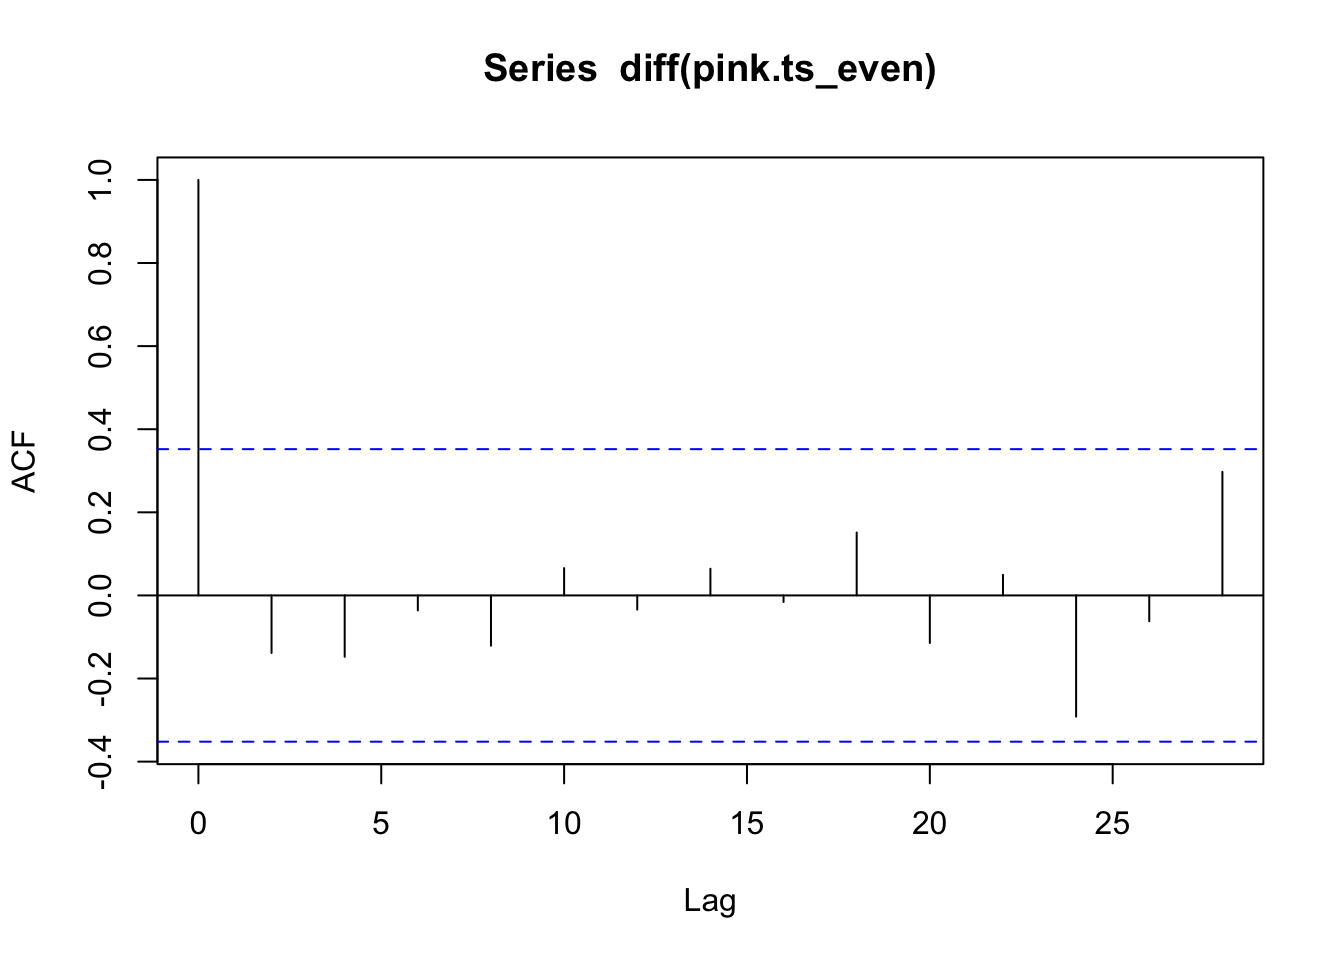
\includegraphics{Lab-1-Emma-ZR-MHS-draft_files/figure-latex/unnamed-chunk-34-2.pdf}
The differences and the ACF plots here look better than the aggregate
data set. Let's look at a forcast.

\begin{Shaded}
\begin{Highlighting}[]
\CommentTok{\#Train and test for a 10 year period}
\NormalTok{train.pink\_even}\OtherTok{\textless{}{-}}\FunctionTok{window}\NormalTok{(pink.ts\_even, }\AttributeTok{start=}\DecValTok{1952}\NormalTok{, }\AttributeTok{end=}\DecValTok{2004}\NormalTok{)}
\NormalTok{test.pink\_even}\OtherTok{\textless{}{-}}\FunctionTok{window}\NormalTok{(pink.ts\_even, }\AttributeTok{start=}\DecValTok{2006}\NormalTok{, }\AttributeTok{end=}\DecValTok{2014}\NormalTok{)}

\NormalTok{fit }\OtherTok{\textless{}{-}}\NormalTok{ forecast}\SpecialCharTok{::}\FunctionTok{auto.arima}\NormalTok{(train.pink\_even, }\AttributeTok{trace=}\NormalTok{T)}
\end{Highlighting}
\end{Shaded}

\begin{verbatim}
## 
##  ARIMA(2,1,2) with drift         : Inf
##  ARIMA(0,1,0) with drift         : 2.346942
##  ARIMA(1,1,0) with drift         : 4.419114
##  ARIMA(0,1,1) with drift         : 4.222938
##  ARIMA(0,1,0)                    : 0.1554815
##  ARIMA(1,1,1) with drift         : Inf
## 
##  Best model: ARIMA(0,1,0)
\end{verbatim}

\begin{Shaded}
\begin{Highlighting}[]
\NormalTok{fit.final.pink\_even}\OtherTok{\textless{}{-}}\NormalTok{forecast}\SpecialCharTok{::}\FunctionTok{auto.arima}\NormalTok{(train.pink\_even, }\AttributeTok{approximation =}\NormalTok{ F, }\AttributeTok{stepwise =}\NormalTok{ F)}

\NormalTok{fit.final.pink\_even }\SpecialCharTok{\%\textgreater{}\%}
  \FunctionTok{forecast}\NormalTok{(}\AttributeTok{h=}\DecValTok{15}\NormalTok{) }\SpecialCharTok{\%\textgreater{}\%}
  \FunctionTok{autoplot}\NormalTok{() }\SpecialCharTok{+} \FunctionTok{geom\_point}\NormalTok{(}\FunctionTok{aes}\NormalTok{(}\AttributeTok{x=}\NormalTok{x, }\AttributeTok{y=}\NormalTok{y), }\AttributeTok{data=}\FunctionTok{fortify}\NormalTok{(test.pink\_even))}
\end{Highlighting}
\end{Shaded}

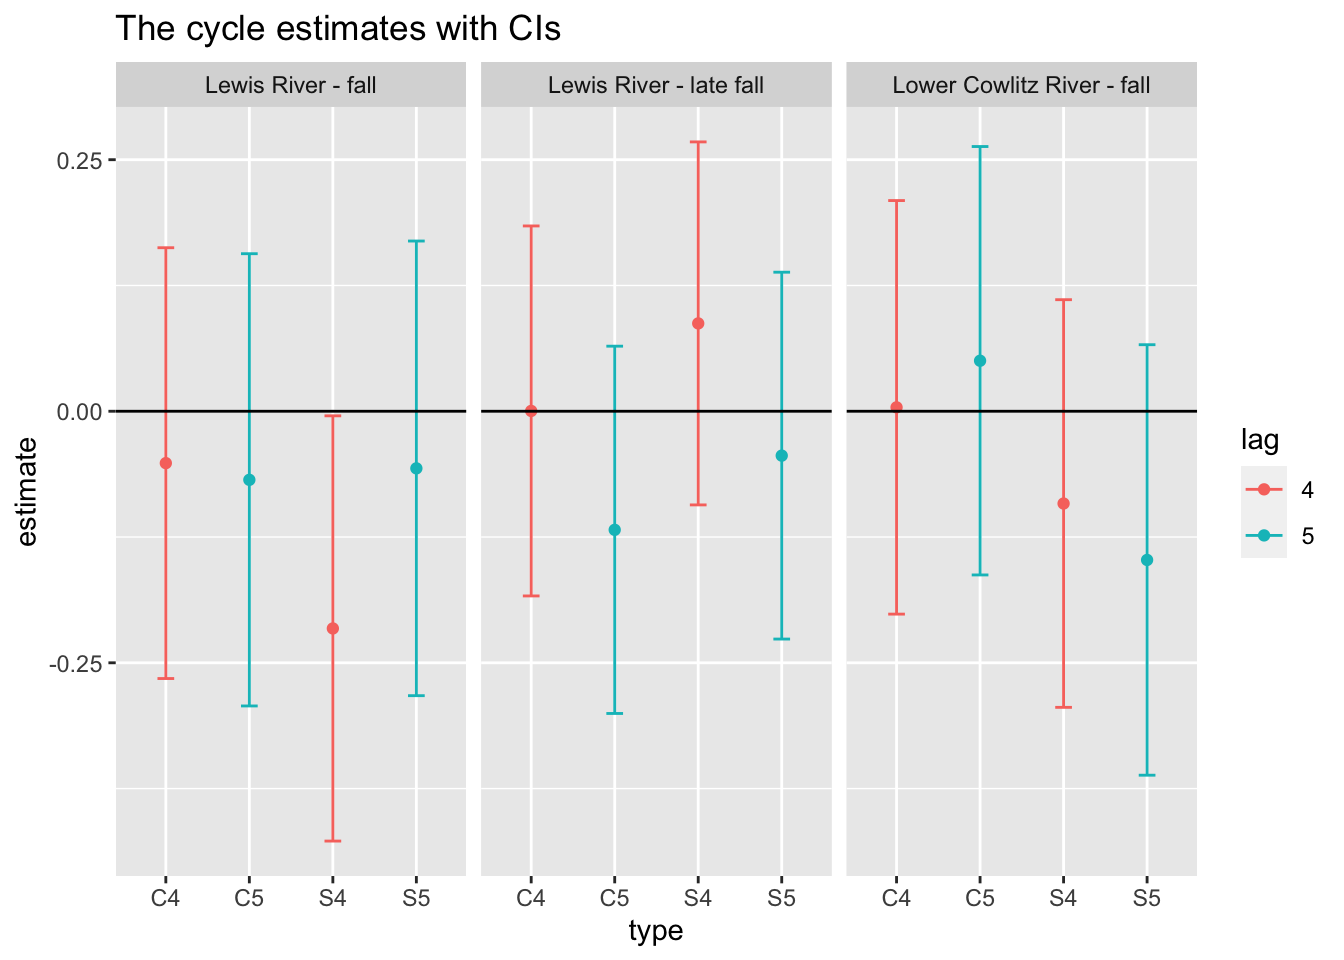
\includegraphics{Lab-1-Emma-ZR-MHS-draft_files/figure-latex/unnamed-chunk-35-1.pdf}

\begin{Shaded}
\begin{Highlighting}[]
\CommentTok{\#That is a straight line..... not very good.....}
\end{Highlighting}
\end{Shaded}

The best model was the ARIMA(0,1,0) model. But the forcast doesn't
capture the trend.

Let's repeat the next steps for odd years.

\begin{Shaded}
\begin{Highlighting}[]
\CommentTok{\#Odd Years {-}{-} Total}

\NormalTok{total.pink\_odd}\OtherTok{\textless{}{-}}\NormalTok{PinkByRegion\_odd }\SpecialCharTok{\%\textgreater{}\%}
  \FunctionTok{group\_by}\NormalTok{(year) }\SpecialCharTok{\%\textgreater{}\%}
  \FunctionTok{summarize}\NormalTok{(}\AttributeTok{lntotal=}\FunctionTok{log}\NormalTok{(}\FunctionTok{sum}\NormalTok{(total, }\AttributeTok{na.rm=}\NormalTok{T)))}

\NormalTok{pink.ts\_odd}\OtherTok{\textless{}{-}}\FunctionTok{ts}\NormalTok{(total.pink\_odd}\SpecialCharTok{$}\NormalTok{lntotal, }
                 \AttributeTok{start=}\NormalTok{total.pink\_odd}\SpecialCharTok{$}\NormalTok{year[}\DecValTok{1}\NormalTok{], }\AttributeTok{frequency =} \FloatTok{0.5}\NormalTok{)}
\FunctionTok{plot}\NormalTok{(}\FunctionTok{diff}\NormalTok{(pink.ts\_odd)) }\CommentTok{\#Looks pretty stationary}
\end{Highlighting}
\end{Shaded}

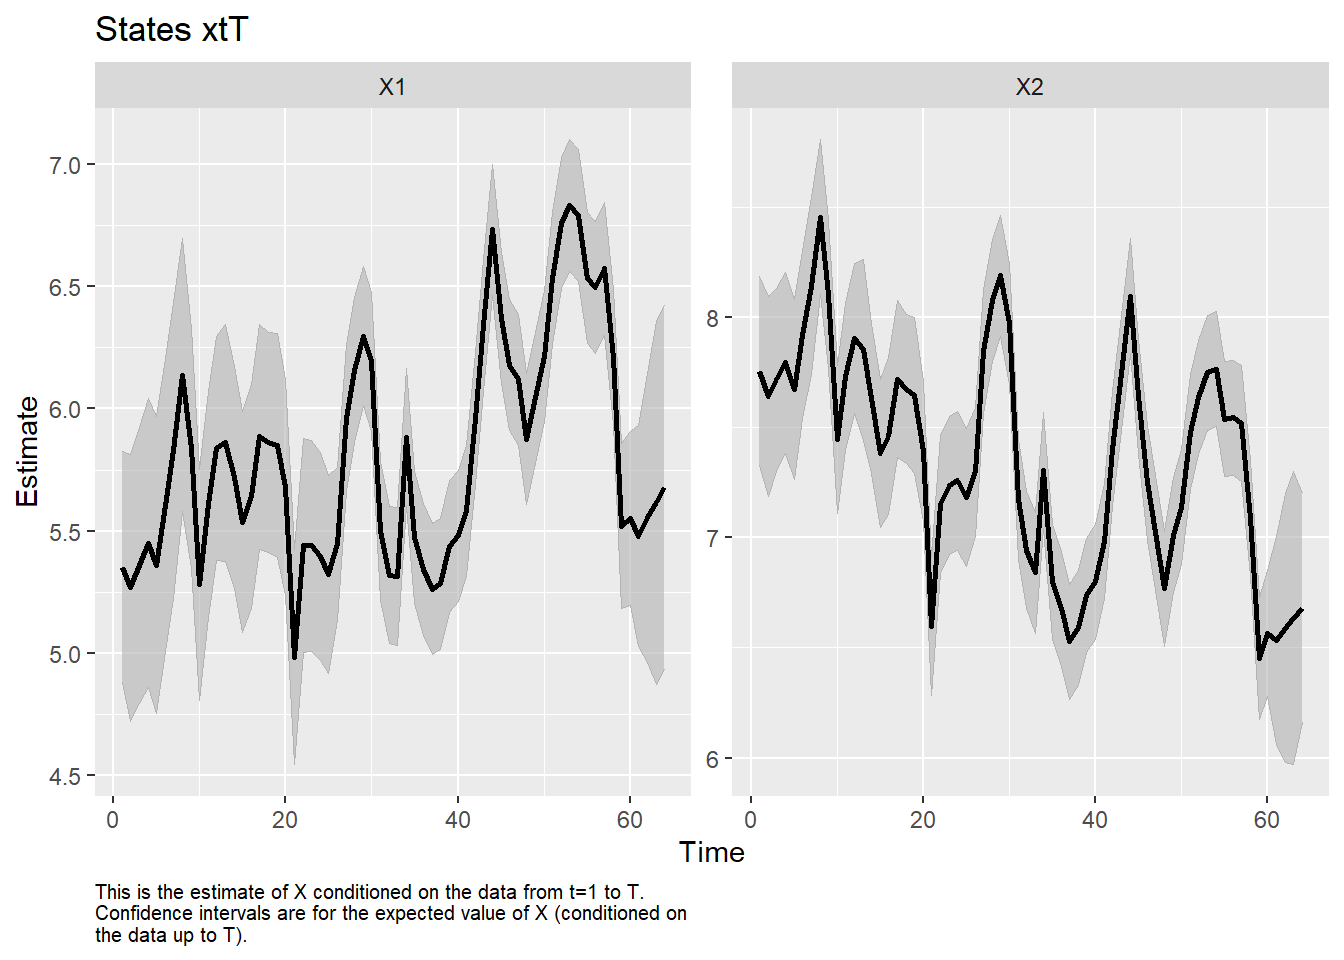
\includegraphics{Lab-1-Emma-ZR-MHS-draft_files/figure-latex/unnamed-chunk-36-1.pdf}

\begin{Shaded}
\begin{Highlighting}[]
\FunctionTok{acf}\NormalTok{(}\FunctionTok{diff}\NormalTok{(pink.ts\_odd)) }\CommentTok{\#This also looks better}
\end{Highlighting}
\end{Shaded}

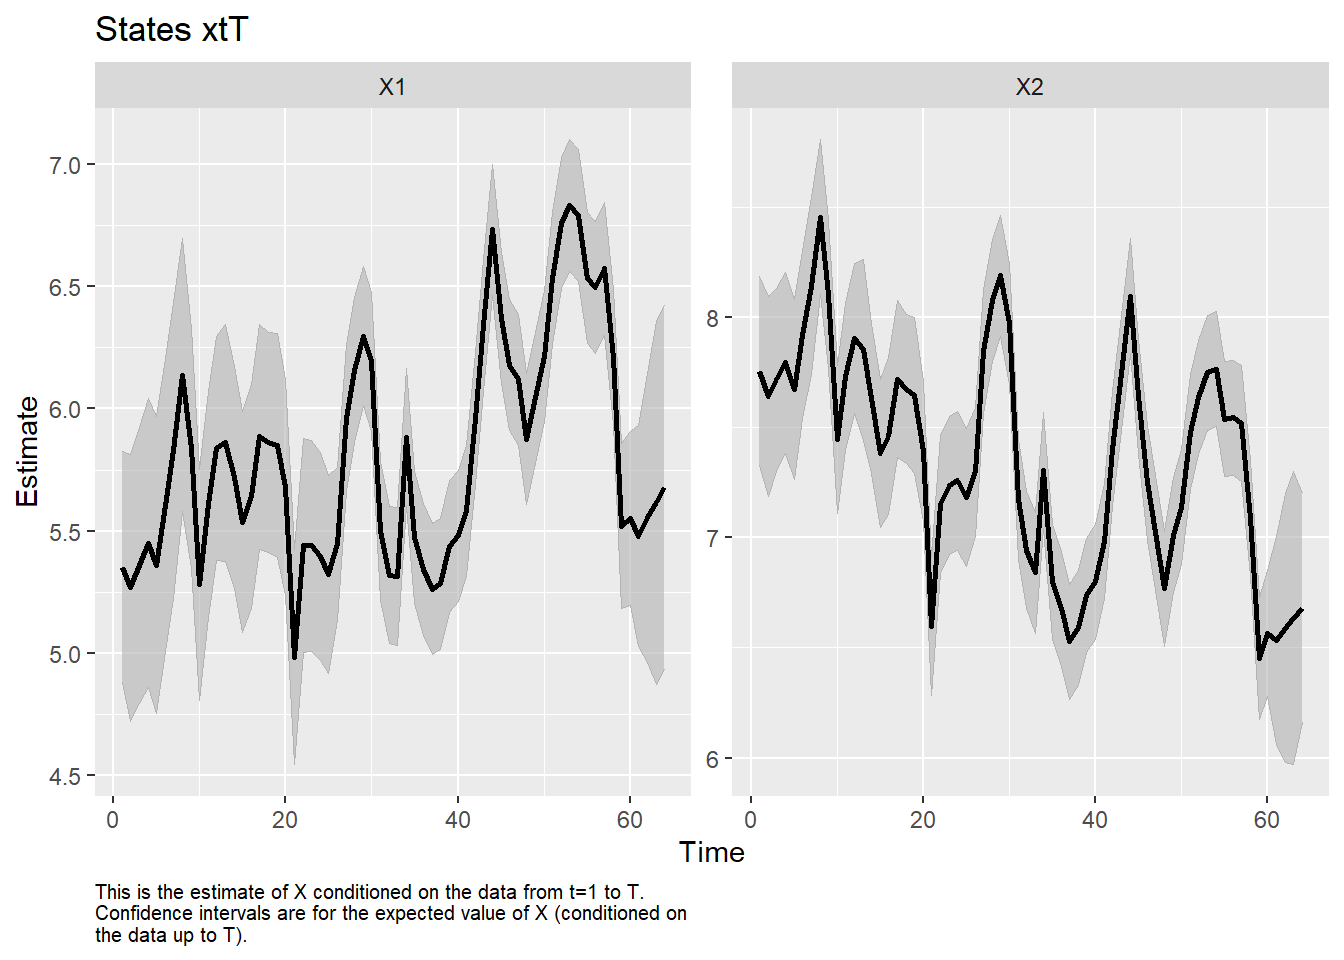
\includegraphics{Lab-1-Emma-ZR-MHS-draft_files/figure-latex/unnamed-chunk-36-2.pdf}
These look stationary and the ACF looks better.

\begin{Shaded}
\begin{Highlighting}[]
\CommentTok{\#Train and test for a 10 year period}
\NormalTok{train.pink\_odd}\OtherTok{\textless{}{-}}\FunctionTok{window}\NormalTok{(pink.ts\_odd, }\AttributeTok{start=}\DecValTok{1953}\NormalTok{, }\AttributeTok{end=}\DecValTok{2005}\NormalTok{)}
\NormalTok{test.pink\_odd}\OtherTok{\textless{}{-}}\FunctionTok{window}\NormalTok{(pink.ts\_odd, }\AttributeTok{start=}\DecValTok{2007}\NormalTok{, }\AttributeTok{end=}\DecValTok{2015}\NormalTok{)}

\NormalTok{fit }\OtherTok{\textless{}{-}}\NormalTok{ forecast}\SpecialCharTok{::}\FunctionTok{auto.arima}\NormalTok{(train.pink\_odd, }\AttributeTok{trace=}\NormalTok{T)}
\end{Highlighting}
\end{Shaded}

\begin{verbatim}
## 
##  ARIMA(2,1,2) with drift         : Inf
##  ARIMA(0,1,0) with drift         : 4.01998
##  ARIMA(1,1,0) with drift         : 5.551776
##  ARIMA(0,1,1) with drift         : 4.461601
##  ARIMA(0,1,0)                    : 1.771054
##  ARIMA(1,1,1) with drift         : Inf
## 
##  Best model: ARIMA(0,1,0)
\end{verbatim}

\begin{Shaded}
\begin{Highlighting}[]
\NormalTok{fit.final.pink\_odd}\OtherTok{\textless{}{-}}\NormalTok{forecast}\SpecialCharTok{::}\FunctionTok{auto.arima}\NormalTok{(train.pink\_odd, }\AttributeTok{approximation =}\NormalTok{ F, }\AttributeTok{stepwise =}\NormalTok{ F)}

\NormalTok{fit.final.pink\_odd }\SpecialCharTok{\%\textgreater{}\%}
  \FunctionTok{forecast}\NormalTok{(}\AttributeTok{h=}\DecValTok{15}\NormalTok{) }\SpecialCharTok{\%\textgreater{}\%}
  \FunctionTok{autoplot}\NormalTok{() }\SpecialCharTok{+} \FunctionTok{geom\_point}\NormalTok{(}\FunctionTok{aes}\NormalTok{(}\AttributeTok{x=}\NormalTok{x, }\AttributeTok{y=}\NormalTok{y), }\AttributeTok{data=}\FunctionTok{fortify}\NormalTok{(test.pink\_odd))}
\end{Highlighting}
\end{Shaded}

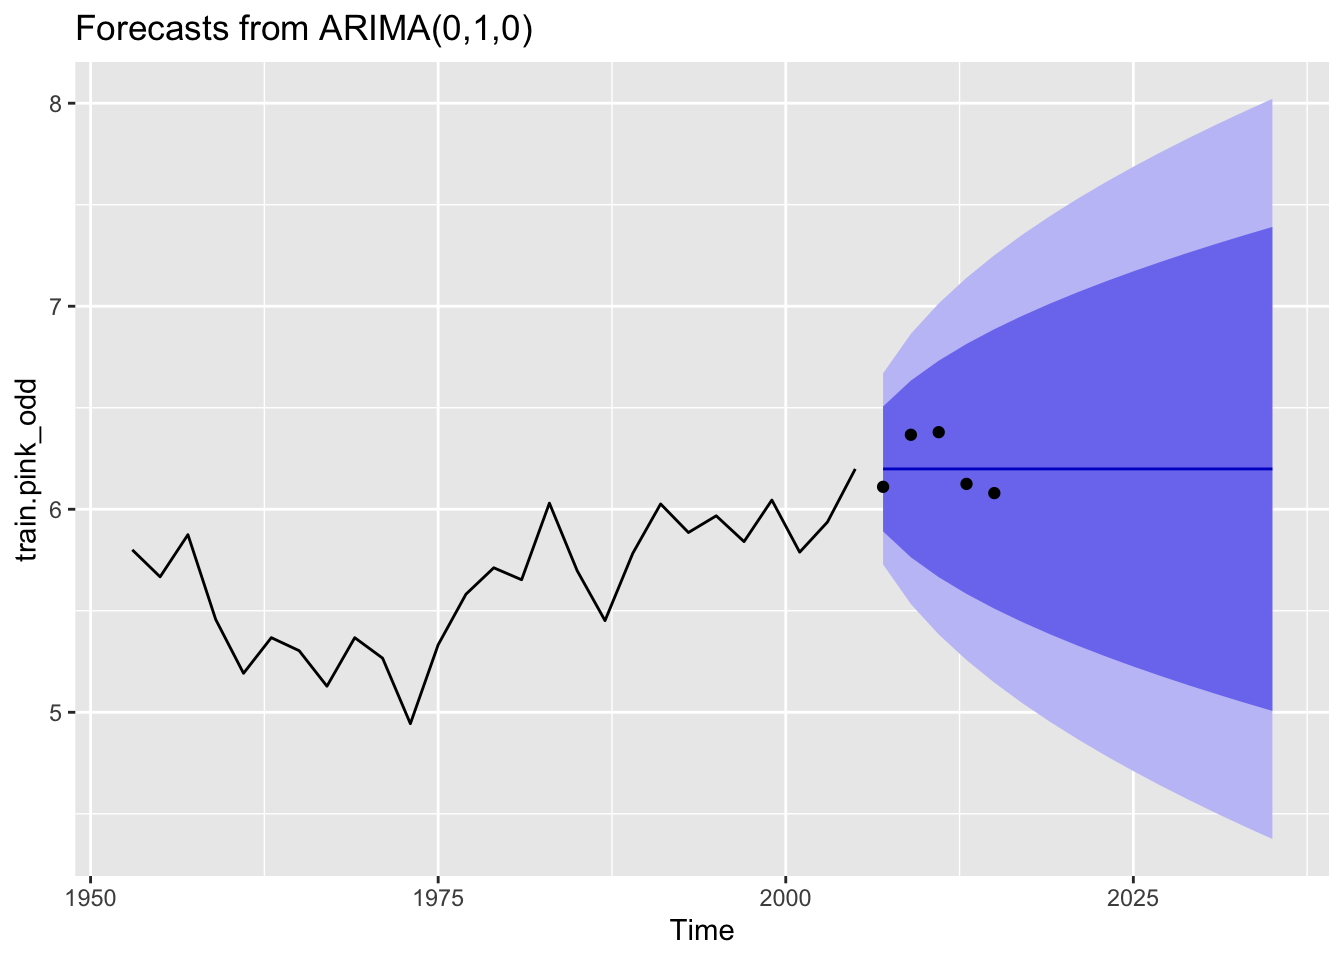
\includegraphics{Lab-1-Emma-ZR-MHS-draft_files/figure-latex/unnamed-chunk-37-1.pdf}
The best model was the ARIMA(0,1,0) model. But the forcast for only odd
years also doesn't capture the trend.

\hypertarget{pinks-regional-considerations}{%
\section{Pinks: Regional
Considerations}\label{pinks-regional-considerations}}

Because of pink salmon life history, for regional models, models with
even and odd years were considered separately.

\begin{Shaded}
\begin{Highlighting}[]
\CommentTok{\#Even Years First }
\CommentTok{\#Differenced plots for all Regions }
\NormalTok{PinkByRegion\_even }\SpecialCharTok{\%\textgreater{}\%}
  \FunctionTok{group\_by}\NormalTok{(region) }\SpecialCharTok{\%\textgreater{}\%}
  \FunctionTok{mutate}\NormalTok{(}\AttributeTok{diff\_total =} \FunctionTok{c}\NormalTok{(}\ConstantTok{NA}\NormalTok{, }\FunctionTok{diff}\NormalTok{(total))) }\SpecialCharTok{\%\textgreater{}\%}
  \FunctionTok{ggplot}\NormalTok{(}\FunctionTok{aes}\NormalTok{(}\AttributeTok{x =}\NormalTok{ year, }\AttributeTok{y =}\NormalTok{ diff\_total)) }\SpecialCharTok{+}
  \FunctionTok{geom\_line}\NormalTok{() }\SpecialCharTok{+}
  \FunctionTok{facet\_wrap}\NormalTok{(}\SpecialCharTok{\textasciitilde{}}\NormalTok{region, }\AttributeTok{scales =} \StringTok{"free\_y"}\NormalTok{) }\SpecialCharTok{+}
  \FunctionTok{ylab}\NormalTok{(}\StringTok{"Difference in Total Returns"}\NormalTok{) }\SpecialCharTok{+}
  \FunctionTok{xlab}\NormalTok{(}\StringTok{"Year"}\NormalTok{) }\SpecialCharTok{+}
  \FunctionTok{ggtitle}\NormalTok{(}\StringTok{"Diff by Region (Even Years)"}\NormalTok{) }
\end{Highlighting}
\end{Shaded}

\begin{verbatim}
## Warning: Removed 1 row containing missing values (`geom_line()`).
\end{verbatim}

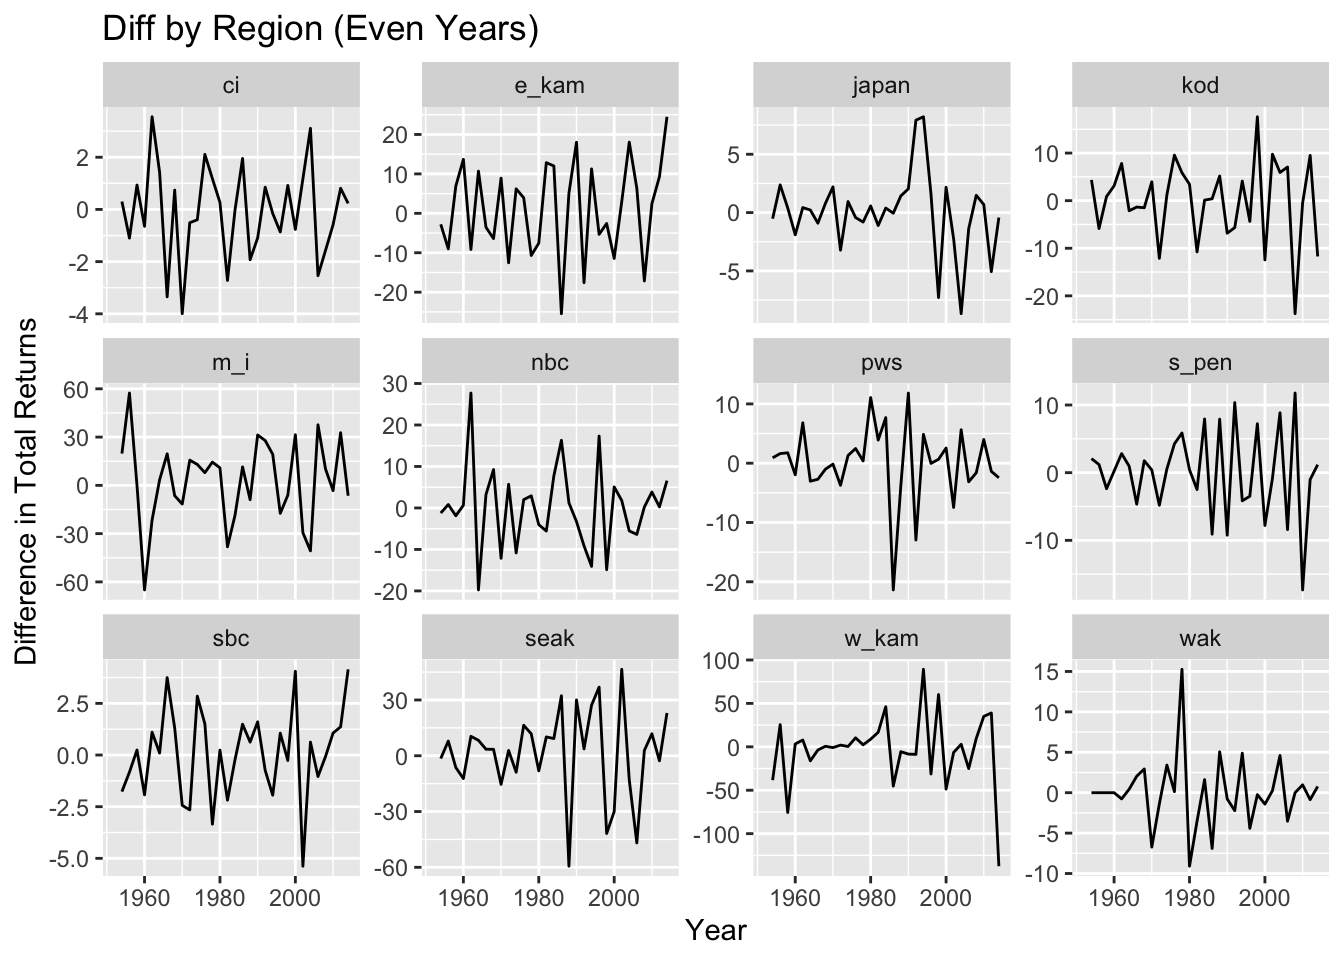
\includegraphics{Lab-1-Emma-ZR-MHS-draft_files/figure-latex/unnamed-chunk-38-1.pdf}

\begin{Shaded}
\begin{Highlighting}[]
  \CommentTok{\#ggfortify::ggstat\_acf(method = "ma", na.action = na.pass)}

\CommentTok{\# Odd Years First }
\CommentTok{\#Differenced plots for all Regions }
\NormalTok{PinkByRegion\_odd }\SpecialCharTok{\%\textgreater{}\%}
  \FunctionTok{group\_by}\NormalTok{(region) }\SpecialCharTok{\%\textgreater{}\%}
  \FunctionTok{mutate}\NormalTok{(}\AttributeTok{diff\_total =} \FunctionTok{c}\NormalTok{(}\ConstantTok{NA}\NormalTok{, }\FunctionTok{diff}\NormalTok{(total))) }\SpecialCharTok{\%\textgreater{}\%}
  \FunctionTok{ggplot}\NormalTok{(}\FunctionTok{aes}\NormalTok{(}\AttributeTok{x =}\NormalTok{ year, }\AttributeTok{y =}\NormalTok{ diff\_total)) }\SpecialCharTok{+}
  \FunctionTok{geom\_line}\NormalTok{() }\SpecialCharTok{+}
  \FunctionTok{facet\_wrap}\NormalTok{(}\SpecialCharTok{\textasciitilde{}}\NormalTok{region, }\AttributeTok{scales =} \StringTok{"free\_y"}\NormalTok{) }\SpecialCharTok{+}
  \FunctionTok{ylab}\NormalTok{(}\StringTok{"Difference in Total Returns"}\NormalTok{) }\SpecialCharTok{+}
  \FunctionTok{xlab}\NormalTok{(}\StringTok{"Year"}\NormalTok{) }\SpecialCharTok{+}
  \FunctionTok{ggtitle}\NormalTok{(}\StringTok{"Diff by Region (Odd Years)"}\NormalTok{) }
\end{Highlighting}
\end{Shaded}

\begin{verbatim}
## Warning: Removed 1 row containing missing values (`geom_line()`).
\end{verbatim}

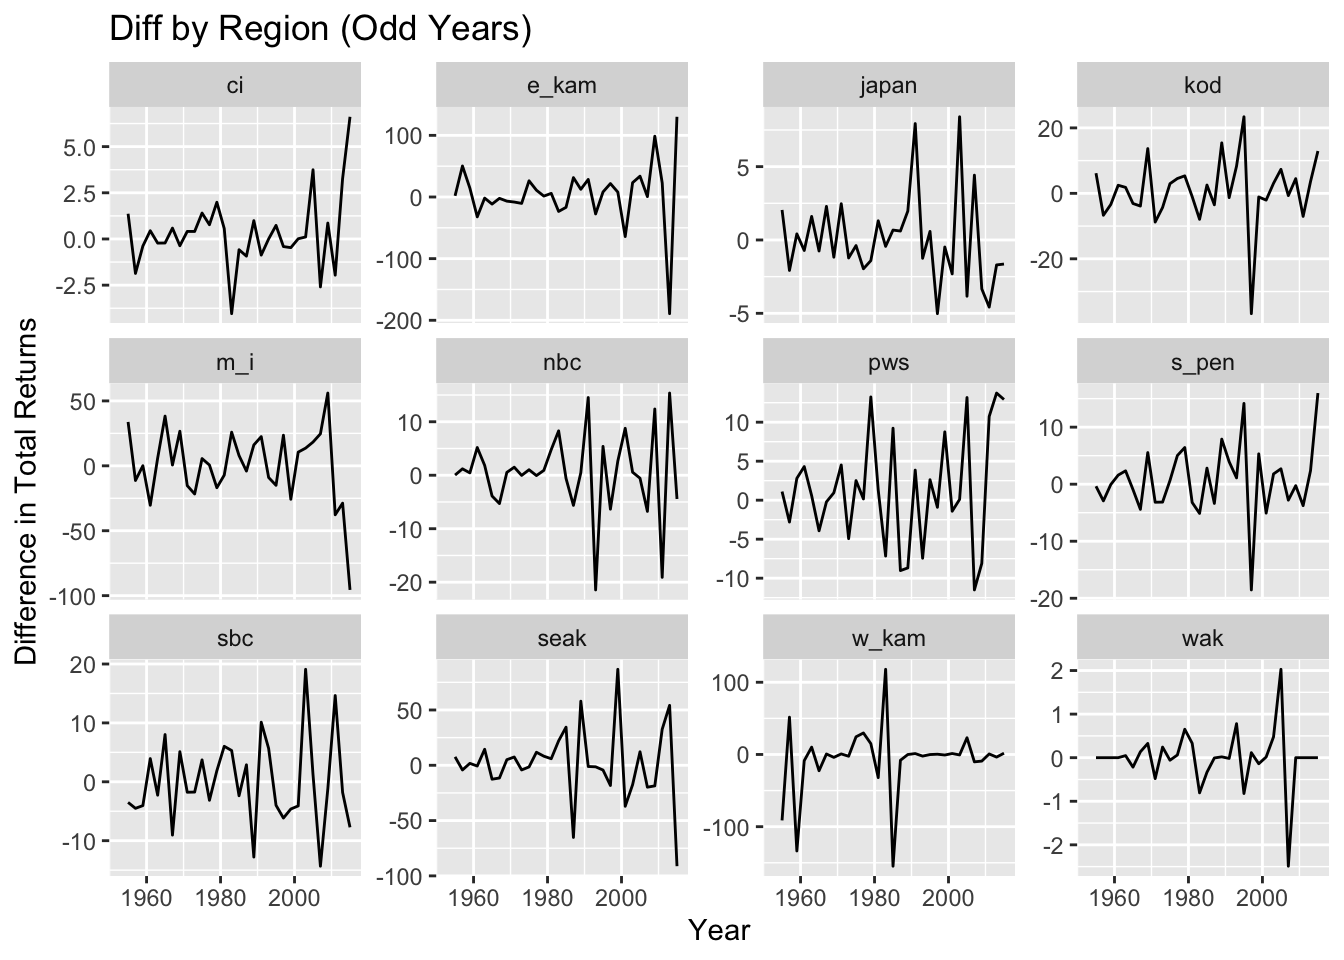
\includegraphics{Lab-1-Emma-ZR-MHS-draft_files/figure-latex/unnamed-chunk-38-2.pdf}
To test stationarity outside the auto.arima function , the ADF and KPSS
tests were compared for all years, and even and odd years. Note for the
ADF null hypothesis is that the system is non-stationary (we want to
reject), and the KPSS test null hypothesis is that there is
stationarity.

\begin{Shaded}
\begin{Highlighting}[]
\CommentTok{\#Augmented Dicky Fuller }
\NormalTok{tseries}\SpecialCharTok{::}\FunctionTok{adf.test}\NormalTok{(pink.ts, }\AttributeTok{k=}\DecValTok{0}\NormalTok{)}
\end{Highlighting}
\end{Shaded}

\begin{verbatim}
## Warning in tseries::adf.test(pink.ts, k = 0): p-value smaller than printed
## p-value
\end{verbatim}

\begin{verbatim}
## 
##  Augmented Dickey-Fuller Test
## 
## data:  pink.ts
## Dickey-Fuller = -6.7912, Lag order = 0, p-value = 0.01
## alternative hypothesis: stationary
\end{verbatim}

\begin{Shaded}
\begin{Highlighting}[]
\NormalTok{tseries}\SpecialCharTok{::}\FunctionTok{adf.test}\NormalTok{(pink.ts\_even, }\AttributeTok{k=}\DecValTok{0}\NormalTok{)}
\end{Highlighting}
\end{Shaded}

\begin{verbatim}
## 
##  Augmented Dickey-Fuller Test
## 
## data:  pink.ts_even
## Dickey-Fuller = -2.7882, Lag order = 0, p-value = 0.2688
## alternative hypothesis: stationary
\end{verbatim}

\begin{Shaded}
\begin{Highlighting}[]
\NormalTok{tseries}\SpecialCharTok{::}\FunctionTok{adf.test}\NormalTok{(pink.ts\_odd, }\AttributeTok{k=}\DecValTok{0}\NormalTok{)}
\end{Highlighting}
\end{Shaded}

\begin{verbatim}
## 
##  Augmented Dickey-Fuller Test
## 
## data:  pink.ts_odd
## Dickey-Fuller = -3.3957, Lag order = 0, p-value = 0.07573
## alternative hypothesis: stationary
\end{verbatim}

\begin{Shaded}
\begin{Highlighting}[]
\NormalTok{tseries}\SpecialCharTok{::}\FunctionTok{kpss.test}\NormalTok{(pink.ts, }\AttributeTok{null =} \FunctionTok{c}\NormalTok{(}\StringTok{"Level"}\NormalTok{, }\StringTok{"Trend"}\NormalTok{))}
\end{Highlighting}
\end{Shaded}

\begin{verbatim}
## Warning in tseries::kpss.test(pink.ts, null = c("Level", "Trend")): p-value
## smaller than printed p-value
\end{verbatim}

\begin{verbatim}
## 
##  KPSS Test for Level Stationarity
## 
## data:  pink.ts
## KPSS Level = 1.2192, Truncation lag parameter = 3, p-value = 0.01
\end{verbatim}

\begin{Shaded}
\begin{Highlighting}[]
\NormalTok{tseries}\SpecialCharTok{::}\FunctionTok{kpss.test}\NormalTok{(pink.ts\_even, }\AttributeTok{null =} \FunctionTok{c}\NormalTok{(}\StringTok{"Level"}\NormalTok{, }\StringTok{"Trend"}\NormalTok{))}
\end{Highlighting}
\end{Shaded}

\begin{verbatim}
## 
##  KPSS Test for Level Stationarity
## 
## data:  pink.ts_even
## KPSS Level = 0.64625, Truncation lag parameter = 3, p-value = 0.01843
\end{verbatim}

\begin{Shaded}
\begin{Highlighting}[]
\NormalTok{tseries}\SpecialCharTok{::}\FunctionTok{kpss.test}\NormalTok{(pink.ts\_odd, }\AttributeTok{null =} \FunctionTok{c}\NormalTok{(}\StringTok{"Level"}\NormalTok{, }\StringTok{"Trend"}\NormalTok{))}
\end{Highlighting}
\end{Shaded}

\begin{verbatim}
## 
##  KPSS Test for Level Stationarity
## 
## data:  pink.ts_odd
## KPSS Level = 0.64278, Truncation lag parameter = 3, p-value = 0.01875
\end{verbatim}

A complication is that the data sets split by even and odd years were
not passing the tests of stationarity. Perhaps other steps should have
been taken.

\begin{Shaded}
\begin{Highlighting}[]
\CommentTok{\#Functions for Regional ACF and PACF }
\CommentTok{\#======================================================}
\NormalTok{ACFandPACF}\OtherTok{\textless{}{-}}\ControlFlowTok{function}\NormalTok{(reg)\{}
\NormalTok{  Pinkdat}\OtherTok{\textless{}{-}}\NormalTok{PinkByRegion }\SpecialCharTok{\%\textgreater{}\%} \FunctionTok{filter}\NormalTok{(region }\SpecialCharTok{==}\NormalTok{ reg)}
  \CommentTok{\#create time series}
\NormalTok{  datts }\OtherTok{\textless{}{-}} \FunctionTok{ts}\NormalTok{(Pinkdat}\SpecialCharTok{$}\NormalTok{lnreturns, }\AttributeTok{start=}\NormalTok{Pinkdat}\SpecialCharTok{$}\NormalTok{year[}\DecValTok{1}\NormalTok{]) }
  \FunctionTok{return}\NormalTok{(}\FunctionTok{list}\NormalTok{(}\AttributeTok{a =} \FunctionTok{acf}\NormalTok{(datts, }\AttributeTok{plot =} \ConstantTok{FALSE}\NormalTok{), }\AttributeTok{p =} \FunctionTok{pacf}\NormalTok{(datts, }\AttributeTok{plot =} \ConstantTok{FALSE}\NormalTok{)))}
\NormalTok{\}}

\NormalTok{ACFandPACF\_even}\OtherTok{\textless{}{-}}\ControlFlowTok{function}\NormalTok{(reg)\{}
\NormalTok{  Pinkdat}\OtherTok{\textless{}{-}}\NormalTok{PinkByRegion\_even }\SpecialCharTok{\%\textgreater{}\%} \FunctionTok{filter}\NormalTok{(region }\SpecialCharTok{==}\NormalTok{ reg)}
  \CommentTok{\#create time series}
\NormalTok{  datts }\OtherTok{\textless{}{-}} \FunctionTok{ts}\NormalTok{(Pinkdat}\SpecialCharTok{$}\NormalTok{lnreturns, }\AttributeTok{start=}\NormalTok{Pinkdat}\SpecialCharTok{$}\NormalTok{year[}\DecValTok{1}\NormalTok{]) }
  \FunctionTok{return}\NormalTok{(}\FunctionTok{list}\NormalTok{(}\AttributeTok{a =} \FunctionTok{acf}\NormalTok{(datts, }\AttributeTok{plot =} \ConstantTok{FALSE}\NormalTok{), }\AttributeTok{p =} \FunctionTok{pacf}\NormalTok{(datts, }\AttributeTok{plot =} \ConstantTok{FALSE}\NormalTok{)))}
\NormalTok{\}}

\NormalTok{ACFandPACF\_odd}\OtherTok{\textless{}{-}}\ControlFlowTok{function}\NormalTok{(reg)\{}
\NormalTok{  Pinkdat}\OtherTok{\textless{}{-}}\NormalTok{PinkByRegion\_odd }\SpecialCharTok{\%\textgreater{}\%} \FunctionTok{filter}\NormalTok{(region }\SpecialCharTok{==}\NormalTok{ reg)}
  \CommentTok{\#create time series}
\NormalTok{  datts }\OtherTok{\textless{}{-}} \FunctionTok{ts}\NormalTok{(Pinkdat}\SpecialCharTok{$}\NormalTok{lnreturns, }\AttributeTok{start=}\NormalTok{Pinkdat}\SpecialCharTok{$}\NormalTok{year[}\DecValTok{1}\NormalTok{]) }
  \FunctionTok{return}\NormalTok{(}\FunctionTok{list}\NormalTok{(}\AttributeTok{a =} \FunctionTok{acf}\NormalTok{(datts, }\AttributeTok{plot =} \ConstantTok{FALSE}\NormalTok{), }\AttributeTok{p =} \FunctionTok{pacf}\NormalTok{(datts, }\AttributeTok{plot =} \ConstantTok{FALSE}\NormalTok{)))}
\NormalTok{\}}

\NormalTok{FitModFunction}\OtherTok{\textless{}{-}}\ControlFlowTok{function}\NormalTok{(reg, forelevel)\{}
  \CommentTok{\#filter region}
\NormalTok{  Pinkdat}\OtherTok{\textless{}{-}}\NormalTok{PinkByRegion }\SpecialCharTok{\%\textgreater{}\%} \FunctionTok{filter}\NormalTok{(region }\SpecialCharTok{==}\NormalTok{ reg)}
  \CommentTok{\#create time series}
\NormalTok{  datts }\OtherTok{\textless{}{-}} \FunctionTok{ts}\NormalTok{(Pinkdat}\SpecialCharTok{$}\NormalTok{lnreturns, }\AttributeTok{start=}\NormalTok{Pinkdat}\SpecialCharTok{$}\NormalTok{year[}\DecValTok{1}\NormalTok{], }\AttributeTok{frequency =} \FloatTok{0.5}\NormalTok{) }\CommentTok{\#set Frequency for 0.5}
\NormalTok{  cutoff}\OtherTok{\textless{}{-}}\DecValTok{2014}\SpecialCharTok{{-}}\NormalTok{forelevel}
\NormalTok{  train }\OtherTok{\textless{}{-}} \FunctionTok{window}\NormalTok{(datts, Pinkdat}\SpecialCharTok{$}\NormalTok{year[}\DecValTok{1}\NormalTok{], cutoff)}
\NormalTok{  test }\OtherTok{\textless{}{-}} \FunctionTok{window}\NormalTok{(datts, cutoff}\SpecialCharTok{+}\DecValTok{1}\NormalTok{, }\DecValTok{2014}\NormalTok{)}
  
\NormalTok{  mod }\OtherTok{\textless{}{-}} \FunctionTok{auto.arima}\NormalTok{(train)}
  \CommentTok{\#testing to be sure that this is the best model (is the best mode the simplest if it is within 2 AIC values?)}
\NormalTok{  trace }\OtherTok{\textless{}{-}} \FunctionTok{capture.output}\NormalTok{(\{}
    \CommentTok{\# assign so it doesn\textquotesingle{}t pollute the output}
\NormalTok{    model }\OtherTok{\textless{}{-}} \FunctionTok{auto.arima}\NormalTok{(datts, }\AttributeTok{trace =} \ConstantTok{TRUE}\NormalTok{)}
\NormalTok{  \})}
\NormalTok{  con    }\OtherTok{\textless{}{-}} \FunctionTok{textConnection}\NormalTok{(trace)}
\NormalTok{  models }\OtherTok{\textless{}{-}} \FunctionTok{read.table}\NormalTok{(con, }\AttributeTok{sep=}\StringTok{":"}\NormalTok{)}
  \FunctionTok{close}\NormalTok{(con)}
  
  \CommentTok{\#getting the "best models" that are within 2 AIC units}
\NormalTok{  BestMods}\OtherTok{\textless{}{-}}\NormalTok{models}\SpecialCharTok{\%\textgreater{}\%} \FunctionTok{filter}\NormalTok{(}\FunctionTok{row\_number}\NormalTok{() }\SpecialCharTok{!=} \FunctionTok{nrow}\NormalTok{(models)) }\SpecialCharTok{\%\textgreater{}\%} \FunctionTok{mutate}\NormalTok{(}\AttributeTok{AIC =} \FunctionTok{replace}\NormalTok{(V2, V2 }\SpecialCharTok{==} \StringTok{"Inf"}\NormalTok{, }\DecValTok{99999}\NormalTok{), }\AttributeTok{AIC =} \FunctionTok{as.numeric}\NormalTok{(AIC), }\AttributeTok{DeltaAIC =}\NormalTok{ AIC}\SpecialCharTok{{-}}\FunctionTok{min}\NormalTok{(AIC)) }\SpecialCharTok{\%\textgreater{}\%} \FunctionTok{filter}\NormalTok{(DeltaAIC }\SpecialCharTok{\textless{}=} \FloatTok{2.0}\NormalTok{)}
  \ControlFlowTok{for}\NormalTok{(i }\ControlFlowTok{in} \DecValTok{1}\SpecialCharTok{:}\FunctionTok{nrow}\NormalTok{(BestMods))\{}
\NormalTok{    BestMods}\SpecialCharTok{$}\NormalTok{Mod[i]}\OtherTok{\textless{}{-}}\FunctionTok{strsplit}\NormalTok{(}\FunctionTok{strsplit}\NormalTok{(}\FunctionTok{strsplit}\NormalTok{(BestMods}\SpecialCharTok{$}\NormalTok{V1[i], }\StringTok{"[(]"}\NormalTok{)[[}\DecValTok{1}\NormalTok{]][}\DecValTok{2}\NormalTok{], }\StringTok{"[)]"}\NormalTok{)[[}\DecValTok{1}\NormalTok{]][}\DecValTok{1}\NormalTok{],}\StringTok{"[,]"}\NormalTok{)}
\NormalTok{    BestMods}\SpecialCharTok{$}\NormalTok{npar[i]}\OtherTok{\textless{}{-}}\FunctionTok{sum}\NormalTok{(}\FunctionTok{as.numeric}\NormalTok{(BestMods}\SpecialCharTok{$}\NormalTok{Mod[i][[}\DecValTok{1}\NormalTok{]][}\FunctionTok{c}\NormalTok{(}\DecValTok{1}\NormalTok{,}\DecValTok{3}\NormalTok{)]))}
    \ControlFlowTok{if}\NormalTok{(}\FunctionTok{strsplit}\NormalTok{(}\FunctionTok{strsplit}\NormalTok{(BestMods}\SpecialCharTok{$}\NormalTok{V1[i], }\StringTok{"[(]"}\NormalTok{)[[}\DecValTok{1}\NormalTok{]][}\DecValTok{2}\NormalTok{], }\StringTok{"[)]"}\NormalTok{)[[}\DecValTok{1}\NormalTok{]][}\DecValTok{2}\NormalTok{] }\SpecialCharTok{==} \StringTok{" with drift         "}\NormalTok{)\{}
\NormalTok{      BestMods}\SpecialCharTok{$}\NormalTok{npar[i] }\OtherTok{=}\NormalTok{ BestMods}\SpecialCharTok{$}\NormalTok{npar[i] }\SpecialCharTok{+} \DecValTok{1}
\NormalTok{    \}}
\NormalTok{  \}}
  
\NormalTok{  New}\OtherTok{\textless{}{-}}\NormalTok{BestMods }\SpecialCharTok{\%\textgreater{}\%} \FunctionTok{filter}\NormalTok{(npar }\SpecialCharTok{==} \FunctionTok{min}\NormalTok{(npar))}
  \ControlFlowTok{if}\NormalTok{(}\DecValTok{0} \SpecialCharTok{\%in\%}\NormalTok{ New}\SpecialCharTok{$}\NormalTok{DeltaAIC)\{}
    \CommentTok{\#auto arima picked the best model}
\NormalTok{    res}\OtherTok{\textless{}{-}}\FunctionTok{accuracy}\NormalTok{(}\FunctionTok{forecast}\NormalTok{(mod, }\AttributeTok{h=}\NormalTok{forelevel), test)[}\DecValTok{2}\NormalTok{,}\StringTok{"MASE"}\NormalTok{] }\CommentTok{\#test set MASE}
\NormalTok{  \}}\ControlFlowTok{else}\NormalTok{\{}
    \CommentTok{\#of the models with the fewest parameters, pick the lowest AIC}
\NormalTok{    newmod}\OtherTok{\textless{}{-}}\NormalTok{New }\SpecialCharTok{\%\textgreater{}\%} \FunctionTok{filter}\NormalTok{(AIC }\SpecialCharTok{==} \FunctionTok{min}\NormalTok{(AIC)) }\SpecialCharTok{\%\textgreater{}\%} \FunctionTok{select}\NormalTok{(Mod)}
\NormalTok{    mod}\OtherTok{\textless{}{-}}\FunctionTok{Arima}\NormalTok{(train, }\AttributeTok{order =} \FunctionTok{as.numeric}\NormalTok{(}\FunctionTok{strsplit}\NormalTok{(newmod}\SpecialCharTok{$}\NormalTok{Mod[[}\DecValTok{1}\NormalTok{]], }\StringTok{"[,]"}\NormalTok{)), }\AttributeTok{include.constant =} \ConstantTok{TRUE}\NormalTok{)}
\NormalTok{    res}\OtherTok{\textless{}{-}}\FunctionTok{accuracy}\NormalTok{(}\FunctionTok{forecast}\NormalTok{(mod, }\AttributeTok{h=}\NormalTok{forelevel), test)[}\DecValTok{2}\NormalTok{,}\StringTok{"MASE"}\NormalTok{] }\CommentTok{\#test set MASE}
\NormalTok{  \}}
  
  \FunctionTok{return}\NormalTok{(}\FunctionTok{list}\NormalTok{(}\AttributeTok{Fit =}\NormalTok{ mod, }\AttributeTok{MASE =}\NormalTok{ res, }\AttributeTok{Bm =}\NormalTok{ BestMods)) }\CommentTok{\#include best mods for testing to see that it\textquotesingle{}s doing what I want}
  
\NormalTok{\}}

\NormalTok{FitModFunction\_even}\OtherTok{\textless{}{-}}\ControlFlowTok{function}\NormalTok{(reg, forelevel)\{}
  \CommentTok{\#filter region}
\NormalTok{  Pinkdat}\OtherTok{\textless{}{-}}\NormalTok{PinkByRegion\_even }\SpecialCharTok{\%\textgreater{}\%} \FunctionTok{filter}\NormalTok{(region }\SpecialCharTok{==}\NormalTok{ reg)}
  \CommentTok{\#create time series}
\NormalTok{  datts }\OtherTok{\textless{}{-}} \FunctionTok{ts}\NormalTok{(Pinkdat}\SpecialCharTok{$}\NormalTok{lnreturns, }\AttributeTok{start=}\NormalTok{Pinkdat}\SpecialCharTok{$}\NormalTok{year[}\DecValTok{1}\NormalTok{], }\AttributeTok{frequency =} \FloatTok{0.5}\NormalTok{) }\CommentTok{\#set Frequency for 0.5}
\NormalTok{  cutoff}\OtherTok{\textless{}{-}}\DecValTok{2014}\SpecialCharTok{{-}}\NormalTok{forelevel}
\NormalTok{  train }\OtherTok{\textless{}{-}} \FunctionTok{window}\NormalTok{(datts, Pinkdat}\SpecialCharTok{$}\NormalTok{year[}\DecValTok{1}\NormalTok{], cutoff)}
\NormalTok{  test }\OtherTok{\textless{}{-}} \FunctionTok{window}\NormalTok{(datts, cutoff}\SpecialCharTok{+}\DecValTok{1}\NormalTok{, }\DecValTok{2014}\NormalTok{)}
  
\NormalTok{  mod }\OtherTok{\textless{}{-}} \FunctionTok{auto.arima}\NormalTok{(train)}
  \CommentTok{\#testing to be sure that this is the best model (is the best mode the simplest if it is within 2 AIC values?)}
\NormalTok{  trace }\OtherTok{\textless{}{-}} \FunctionTok{capture.output}\NormalTok{(\{}
    \CommentTok{\# assign so it doesn\textquotesingle{}t pollute the output}
\NormalTok{    model }\OtherTok{\textless{}{-}} \FunctionTok{auto.arima}\NormalTok{(datts, }\AttributeTok{trace =} \ConstantTok{TRUE}\NormalTok{)}
\NormalTok{  \})}
\NormalTok{  con    }\OtherTok{\textless{}{-}} \FunctionTok{textConnection}\NormalTok{(trace)}
\NormalTok{  models }\OtherTok{\textless{}{-}} \FunctionTok{read.table}\NormalTok{(con, }\AttributeTok{sep=}\StringTok{":"}\NormalTok{)}
  \FunctionTok{close}\NormalTok{(con)}
  
  \CommentTok{\#getting the "best models" that are within 2 AIC units}
\NormalTok{  BestMods}\OtherTok{\textless{}{-}}\NormalTok{models}\SpecialCharTok{\%\textgreater{}\%} \FunctionTok{filter}\NormalTok{(}\FunctionTok{row\_number}\NormalTok{() }\SpecialCharTok{!=} \FunctionTok{nrow}\NormalTok{(models)) }\SpecialCharTok{\%\textgreater{}\%} \FunctionTok{mutate}\NormalTok{(}\AttributeTok{AIC =} \FunctionTok{replace}\NormalTok{(V2, V2 }\SpecialCharTok{==} \StringTok{"Inf"}\NormalTok{, }\DecValTok{99999}\NormalTok{), }\AttributeTok{AIC =} \FunctionTok{as.numeric}\NormalTok{(AIC), }\AttributeTok{DeltaAIC =}\NormalTok{ AIC}\SpecialCharTok{{-}}\FunctionTok{min}\NormalTok{(AIC)) }\SpecialCharTok{\%\textgreater{}\%} \FunctionTok{filter}\NormalTok{(DeltaAIC }\SpecialCharTok{\textless{}=} \FloatTok{2.0}\NormalTok{)}
  \ControlFlowTok{for}\NormalTok{(i }\ControlFlowTok{in} \DecValTok{1}\SpecialCharTok{:}\FunctionTok{nrow}\NormalTok{(BestMods))\{}
\NormalTok{    BestMods}\SpecialCharTok{$}\NormalTok{Mod[i]}\OtherTok{\textless{}{-}}\FunctionTok{strsplit}\NormalTok{(}\FunctionTok{strsplit}\NormalTok{(}\FunctionTok{strsplit}\NormalTok{(BestMods}\SpecialCharTok{$}\NormalTok{V1[i], }\StringTok{"[(]"}\NormalTok{)[[}\DecValTok{1}\NormalTok{]][}\DecValTok{2}\NormalTok{], }\StringTok{"[)]"}\NormalTok{)[[}\DecValTok{1}\NormalTok{]][}\DecValTok{1}\NormalTok{],}\StringTok{"[,]"}\NormalTok{)}
\NormalTok{    BestMods}\SpecialCharTok{$}\NormalTok{npar[i]}\OtherTok{\textless{}{-}}\FunctionTok{sum}\NormalTok{(}\FunctionTok{as.numeric}\NormalTok{(BestMods}\SpecialCharTok{$}\NormalTok{Mod[i][[}\DecValTok{1}\NormalTok{]][}\FunctionTok{c}\NormalTok{(}\DecValTok{1}\NormalTok{,}\DecValTok{3}\NormalTok{)]))}
    \ControlFlowTok{if}\NormalTok{(}\FunctionTok{strsplit}\NormalTok{(}\FunctionTok{strsplit}\NormalTok{(BestMods}\SpecialCharTok{$}\NormalTok{V1[i], }\StringTok{"[(]"}\NormalTok{)[[}\DecValTok{1}\NormalTok{]][}\DecValTok{2}\NormalTok{], }\StringTok{"[)]"}\NormalTok{)[[}\DecValTok{1}\NormalTok{]][}\DecValTok{2}\NormalTok{] }\SpecialCharTok{==} \StringTok{" with drift         "}\NormalTok{)\{}
\NormalTok{      BestMods}\SpecialCharTok{$}\NormalTok{npar[i] }\OtherTok{=}\NormalTok{ BestMods}\SpecialCharTok{$}\NormalTok{npar[i] }\SpecialCharTok{+} \DecValTok{1}
\NormalTok{    \}}
\NormalTok{  \}}
  
\NormalTok{  New}\OtherTok{\textless{}{-}}\NormalTok{BestMods }\SpecialCharTok{\%\textgreater{}\%} \FunctionTok{filter}\NormalTok{(npar }\SpecialCharTok{==} \FunctionTok{min}\NormalTok{(npar))}
  \ControlFlowTok{if}\NormalTok{(}\DecValTok{0} \SpecialCharTok{\%in\%}\NormalTok{ New}\SpecialCharTok{$}\NormalTok{DeltaAIC)\{}
    \CommentTok{\#auto arima picked the best model}
\NormalTok{    res}\OtherTok{\textless{}{-}}\FunctionTok{accuracy}\NormalTok{(}\FunctionTok{forecast}\NormalTok{(mod, }\AttributeTok{h=}\NormalTok{forelevel), test)[}\DecValTok{2}\NormalTok{,}\StringTok{"MASE"}\NormalTok{] }\CommentTok{\#test set MASE}
\NormalTok{  \}}\ControlFlowTok{else}\NormalTok{\{}
    \CommentTok{\#of the models with the fewest parameters, pick the lowest AIC}
\NormalTok{    newmod}\OtherTok{\textless{}{-}}\NormalTok{New }\SpecialCharTok{\%\textgreater{}\%} \FunctionTok{filter}\NormalTok{(AIC }\SpecialCharTok{==} \FunctionTok{min}\NormalTok{(AIC)) }\SpecialCharTok{\%\textgreater{}\%} \FunctionTok{select}\NormalTok{(Mod)}
\NormalTok{    mod}\OtherTok{\textless{}{-}}\FunctionTok{Arima}\NormalTok{(train, }\AttributeTok{order =} \FunctionTok{as.numeric}\NormalTok{(}\FunctionTok{strsplit}\NormalTok{(newmod}\SpecialCharTok{$}\NormalTok{Mod[[}\DecValTok{1}\NormalTok{]], }\StringTok{"[,]"}\NormalTok{)), }\AttributeTok{include.constant =} \ConstantTok{TRUE}\NormalTok{)}
\NormalTok{    res}\OtherTok{\textless{}{-}}\FunctionTok{accuracy}\NormalTok{(}\FunctionTok{forecast}\NormalTok{(mod, }\AttributeTok{h=}\NormalTok{forelevel), test)[}\DecValTok{2}\NormalTok{,}\StringTok{"MASE"}\NormalTok{] }\CommentTok{\#test set MASE}
\NormalTok{  \}}
  
  \FunctionTok{return}\NormalTok{(}\FunctionTok{list}\NormalTok{(}\AttributeTok{Fit =}\NormalTok{ mod, }\AttributeTok{MASE =}\NormalTok{ res, }\AttributeTok{Bm =}\NormalTok{ BestMods)) }\CommentTok{\#include best mods for testing to see that it\textquotesingle{}s doing what I want}
  
\NormalTok{\}}

\NormalTok{FitModFunction\_odd}\OtherTok{\textless{}{-}}\ControlFlowTok{function}\NormalTok{(reg, forelevel)\{}
  \CommentTok{\#filter region}
\NormalTok{  Pinkdat}\OtherTok{\textless{}{-}}\NormalTok{PinkByRegion\_odd }\SpecialCharTok{\%\textgreater{}\%} \FunctionTok{filter}\NormalTok{(region }\SpecialCharTok{==}\NormalTok{ reg)}
  \CommentTok{\#create time series}
\NormalTok{  datts }\OtherTok{\textless{}{-}} \FunctionTok{ts}\NormalTok{(Pinkdat}\SpecialCharTok{$}\NormalTok{lnreturns, }\AttributeTok{start=}\NormalTok{Pinkdat}\SpecialCharTok{$}\NormalTok{year[}\DecValTok{1}\NormalTok{], }\AttributeTok{frequency =} \FloatTok{0.5}\NormalTok{) }
\NormalTok{  cutoff}\OtherTok{\textless{}{-}}\DecValTok{2015}\SpecialCharTok{{-}}\NormalTok{forelevel}
\NormalTok{  train }\OtherTok{\textless{}{-}} \FunctionTok{window}\NormalTok{(datts, Pinkdat}\SpecialCharTok{$}\NormalTok{year[}\DecValTok{1}\NormalTok{], cutoff)}
\NormalTok{  test }\OtherTok{\textless{}{-}} \FunctionTok{window}\NormalTok{(datts, cutoff}\SpecialCharTok{+}\DecValTok{1}\NormalTok{, }\DecValTok{2015}\NormalTok{)}
  
\NormalTok{  mod }\OtherTok{\textless{}{-}} \FunctionTok{auto.arima}\NormalTok{(train)}
  \CommentTok{\#testing to be sure that this is the best model (is the best mode the simplest if it is within 2 AIC values?)}
\NormalTok{  trace }\OtherTok{\textless{}{-}} \FunctionTok{capture.output}\NormalTok{(\{}
    \CommentTok{\# assign so it doesn\textquotesingle{}t pollute the output}
\NormalTok{    model }\OtherTok{\textless{}{-}} \FunctionTok{auto.arima}\NormalTok{(datts, }\AttributeTok{trace =} \ConstantTok{TRUE}\NormalTok{)}
\NormalTok{  \})}
\NormalTok{  con    }\OtherTok{\textless{}{-}} \FunctionTok{textConnection}\NormalTok{(trace)}
\NormalTok{  models }\OtherTok{\textless{}{-}} \FunctionTok{read.table}\NormalTok{(con, }\AttributeTok{sep=}\StringTok{":"}\NormalTok{)}
  \FunctionTok{close}\NormalTok{(con)}
  
  \CommentTok{\#getting the "best models" that are within 2 AIC units}
\NormalTok{  BestMods}\OtherTok{\textless{}{-}}\NormalTok{models}\SpecialCharTok{\%\textgreater{}\%} \FunctionTok{filter}\NormalTok{(}\FunctionTok{row\_number}\NormalTok{() }\SpecialCharTok{!=} \FunctionTok{nrow}\NormalTok{(models)) }\SpecialCharTok{\%\textgreater{}\%} \FunctionTok{mutate}\NormalTok{(}\AttributeTok{AIC =} \FunctionTok{replace}\NormalTok{(V2, V2 }\SpecialCharTok{==} \StringTok{"Inf"}\NormalTok{, }\DecValTok{99999}\NormalTok{), }\AttributeTok{AIC =} \FunctionTok{as.numeric}\NormalTok{(AIC), }\AttributeTok{DeltaAIC =}\NormalTok{ AIC}\SpecialCharTok{{-}}\FunctionTok{min}\NormalTok{(AIC)) }\SpecialCharTok{\%\textgreater{}\%} \FunctionTok{filter}\NormalTok{(DeltaAIC }\SpecialCharTok{\textless{}=} \FloatTok{2.0}\NormalTok{)}
  \ControlFlowTok{for}\NormalTok{(i }\ControlFlowTok{in} \DecValTok{1}\SpecialCharTok{:}\FunctionTok{nrow}\NormalTok{(BestMods))\{}
\NormalTok{    BestMods}\SpecialCharTok{$}\NormalTok{Mod[i]}\OtherTok{\textless{}{-}}\FunctionTok{strsplit}\NormalTok{(}\FunctionTok{strsplit}\NormalTok{(}\FunctionTok{strsplit}\NormalTok{(BestMods}\SpecialCharTok{$}\NormalTok{V1[i], }\StringTok{"[(]"}\NormalTok{)[[}\DecValTok{1}\NormalTok{]][}\DecValTok{2}\NormalTok{], }\StringTok{"[)]"}\NormalTok{)[[}\DecValTok{1}\NormalTok{]][}\DecValTok{1}\NormalTok{],}\StringTok{"[,]"}\NormalTok{)}
\NormalTok{    BestMods}\SpecialCharTok{$}\NormalTok{npar[i]}\OtherTok{\textless{}{-}}\FunctionTok{sum}\NormalTok{(}\FunctionTok{as.numeric}\NormalTok{(BestMods}\SpecialCharTok{$}\NormalTok{Mod[i][[}\DecValTok{1}\NormalTok{]][}\FunctionTok{c}\NormalTok{(}\DecValTok{1}\NormalTok{,}\DecValTok{3}\NormalTok{)]))}
    \ControlFlowTok{if}\NormalTok{(}\FunctionTok{strsplit}\NormalTok{(}\FunctionTok{strsplit}\NormalTok{(BestMods}\SpecialCharTok{$}\NormalTok{V1[i], }\StringTok{"[(]"}\NormalTok{)[[}\DecValTok{1}\NormalTok{]][}\DecValTok{2}\NormalTok{], }\StringTok{"[)]"}\NormalTok{)[[}\DecValTok{1}\NormalTok{]][}\DecValTok{2}\NormalTok{] }\SpecialCharTok{==} \StringTok{" with drift         "}\NormalTok{)\{}
\NormalTok{      BestMods}\SpecialCharTok{$}\NormalTok{npar[i] }\OtherTok{=}\NormalTok{ BestMods}\SpecialCharTok{$}\NormalTok{npar[i] }\SpecialCharTok{+} \DecValTok{1}
\NormalTok{    \}}
\NormalTok{  \}}
  
\NormalTok{  New}\OtherTok{\textless{}{-}}\NormalTok{BestMods }\SpecialCharTok{\%\textgreater{}\%} \FunctionTok{filter}\NormalTok{(npar }\SpecialCharTok{==} \FunctionTok{min}\NormalTok{(npar))}
  \ControlFlowTok{if}\NormalTok{(}\DecValTok{0} \SpecialCharTok{\%in\%}\NormalTok{ New}\SpecialCharTok{$}\NormalTok{DeltaAIC)\{}
    \CommentTok{\#auto arima picked the best model}
\NormalTok{    res}\OtherTok{\textless{}{-}}\FunctionTok{accuracy}\NormalTok{(}\FunctionTok{forecast}\NormalTok{(mod, }\AttributeTok{h=}\NormalTok{forelevel), test)[}\DecValTok{2}\NormalTok{,}\StringTok{"MASE"}\NormalTok{] }\CommentTok{\#test set MASE}
\NormalTok{  \}}\ControlFlowTok{else}\NormalTok{\{}
    \CommentTok{\#of the models with the fewest parameters, pick the lowest AIC}
\NormalTok{    newmod}\OtherTok{\textless{}{-}}\NormalTok{New }\SpecialCharTok{\%\textgreater{}\%} \FunctionTok{filter}\NormalTok{(AIC }\SpecialCharTok{==} \FunctionTok{min}\NormalTok{(AIC)) }\SpecialCharTok{\%\textgreater{}\%} \FunctionTok{select}\NormalTok{(Mod)}
\NormalTok{    mod}\OtherTok{\textless{}{-}}\FunctionTok{Arima}\NormalTok{(train, }\AttributeTok{order =} \FunctionTok{as.numeric}\NormalTok{(}\FunctionTok{strsplit}\NormalTok{(newmod}\SpecialCharTok{$}\NormalTok{Mod[[}\DecValTok{1}\NormalTok{]], }\StringTok{"[,]"}\NormalTok{)), }\AttributeTok{include.constant =} \ConstantTok{TRUE}\NormalTok{)}
\NormalTok{    res}\OtherTok{\textless{}{-}}\FunctionTok{accuracy}\NormalTok{(}\FunctionTok{forecast}\NormalTok{(mod, }\AttributeTok{h=}\NormalTok{forelevel), test)[}\DecValTok{2}\NormalTok{,}\StringTok{"MASE"}\NormalTok{] }\CommentTok{\#test set MASE}
\NormalTok{  \}}
  
  \FunctionTok{return}\NormalTok{(}\FunctionTok{list}\NormalTok{(}\AttributeTok{Fit =}\NormalTok{ mod, }\AttributeTok{MASE =}\NormalTok{ res, }\AttributeTok{Bm =}\NormalTok{ BestMods)) }\CommentTok{\#include best mods for testing to see that it\textquotesingle{}s doing what I want}
  
\NormalTok{\}}

\CommentTok{\#================================================================}
\end{Highlighting}
\end{Shaded}

Next step is to then define the regions

\begin{Shaded}
\begin{Highlighting}[]
\CommentTok{\#regions vector}
\NormalTok{regions}\OtherTok{\textless{}{-}}\FunctionTok{unique}\NormalTok{(PinkByRegion}\SpecialCharTok{$}\NormalTok{region)}
\CommentTok{\#regions key}
\NormalTok{regionskey}\OtherTok{\textless{}{-}}\FunctionTok{c}\NormalTok{(}\StringTok{"Cook Inlet"}\NormalTok{, }\StringTok{"E. Kamchatka"}\NormalTok{, }\StringTok{"Japan"}\NormalTok{, }\StringTok{"Kodiak"}\NormalTok{, }\StringTok{"Russia"}\NormalTok{, }\StringTok{"N.British Columbia"}\NormalTok{,}
              \StringTok{"Prince William Sound"}\NormalTok{, }\StringTok{"S. Alaska Pen."}\NormalTok{, }\StringTok{"S. British Columbia"}\NormalTok{, }\StringTok{"SE Alaska"}\NormalTok{, }\StringTok{"W. Kamchatka"}\NormalTok{, }\StringTok{"W. Alaska"}\NormalTok{)}
\FunctionTok{names}\NormalTok{(regionskey)}\OtherTok{\textless{}{-}}\NormalTok{regions }\CommentTok{\#for plotting}

\CommentTok{\#loop through regions/levels}
\CommentTok{\#all}
\NormalTok{DiagPlots}\OtherTok{\textless{}{-}}\FunctionTok{lapply}\NormalTok{(regions, ACFandPACF)}
   \FunctionTok{names}\NormalTok{(DiagPlots)}\OtherTok{\textless{}{-}}\NormalTok{regions}

\CommentTok{\#Even}
\NormalTok{DiagPlots\_even}\OtherTok{\textless{}{-}}\FunctionTok{lapply}\NormalTok{(regions, ACFandPACF\_even)}
   \FunctionTok{names}\NormalTok{(DiagPlots\_even)}\OtherTok{\textless{}{-}}\NormalTok{regions}
   
\CommentTok{\#Odd}
\NormalTok{DiagPlots\_odd}\OtherTok{\textless{}{-}}\FunctionTok{lapply}\NormalTok{(regions, ACFandPACF\_odd)}
   \FunctionTok{names}\NormalTok{(DiagPlots\_odd)}\OtherTok{\textless{}{-}}\NormalTok{regions   }
\end{Highlighting}
\end{Shaded}

Lets look at the regional breakdowns of ACF and PACF, first for all
years:

\begin{Shaded}
\begin{Highlighting}[]
\CommentTok{\#Even Years }
\FunctionTok{par}\NormalTok{(}\AttributeTok{mfrow=}\FunctionTok{c}\NormalTok{(}\DecValTok{3}\NormalTok{,}\DecValTok{4}\NormalTok{))}
\ControlFlowTok{for}\NormalTok{(r }\ControlFlowTok{in} \DecValTok{1}\SpecialCharTok{:}\FunctionTok{length}\NormalTok{(regions))\{}
  \FunctionTok{plot}\NormalTok{(DiagPlots[[r]][[}\DecValTok{1}\NormalTok{]], }\AttributeTok{main =} \FunctionTok{paste0}\NormalTok{(}\StringTok{"Region: "}\NormalTok{, regionskey[r]))}
\NormalTok{\}}
\end{Highlighting}
\end{Shaded}

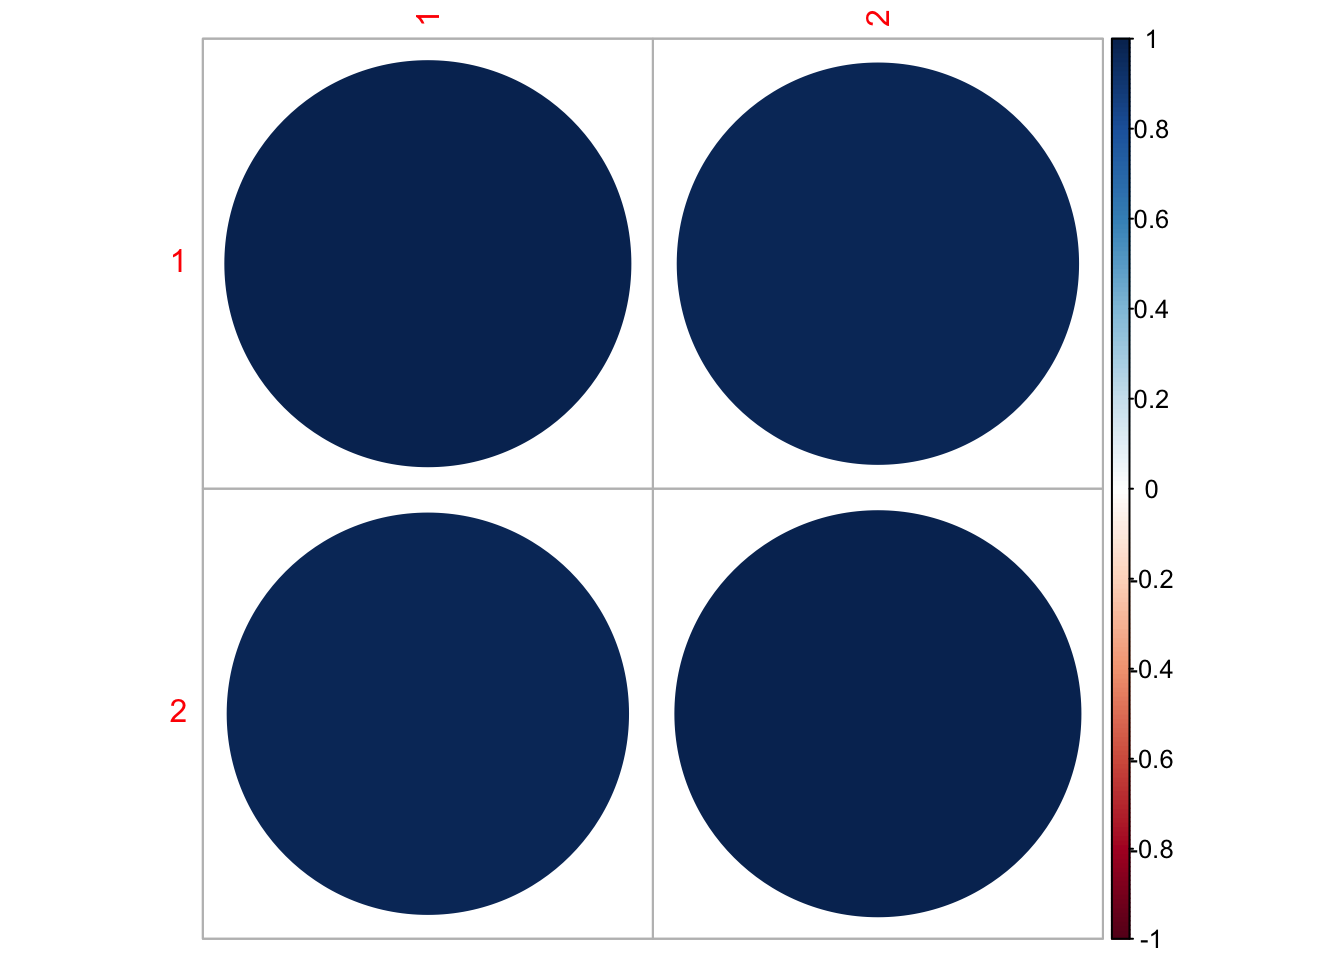
\includegraphics{Lab-1-Emma-ZR-MHS-draft_files/figure-latex/unnamed-chunk-42-1.pdf}

\begin{Shaded}
\begin{Highlighting}[]
\CommentTok{\#PACF plots for each region}
\FunctionTok{par}\NormalTok{(}\AttributeTok{mfrow=}\FunctionTok{c}\NormalTok{(}\DecValTok{3}\NormalTok{,}\DecValTok{4}\NormalTok{))}
\ControlFlowTok{for}\NormalTok{(r }\ControlFlowTok{in} \DecValTok{1}\SpecialCharTok{:}\FunctionTok{length}\NormalTok{(regions))\{}
  \FunctionTok{plot}\NormalTok{(DiagPlots[[r]][[}\DecValTok{2}\NormalTok{]], }\AttributeTok{main =} \FunctionTok{paste0}\NormalTok{(}\StringTok{"Region: "}\NormalTok{, regionskey[r]))}
\NormalTok{\}}
\end{Highlighting}
\end{Shaded}

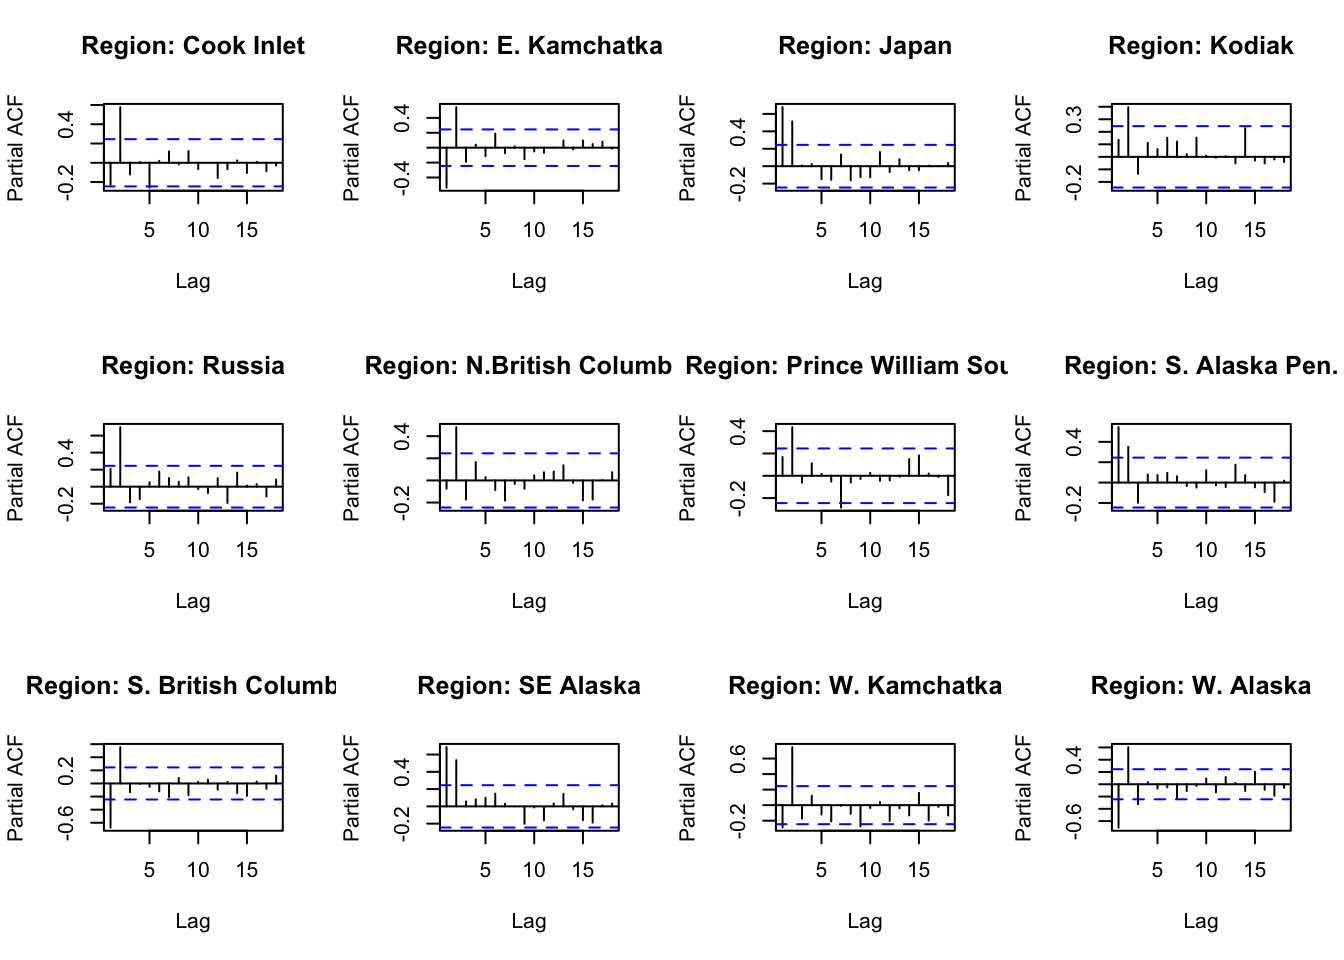
\includegraphics{Lab-1-Emma-ZR-MHS-draft_files/figure-latex/unnamed-chunk-42-2.pdf}
The ACFs for regions show different levels of lag or total correlation.
Let's look for even years:

\begin{Shaded}
\begin{Highlighting}[]
\CommentTok{\#Even Years }
\FunctionTok{par}\NormalTok{(}\AttributeTok{mfrow=}\FunctionTok{c}\NormalTok{(}\DecValTok{3}\NormalTok{,}\DecValTok{4}\NormalTok{))}
\ControlFlowTok{for}\NormalTok{(r }\ControlFlowTok{in} \DecValTok{1}\SpecialCharTok{:}\FunctionTok{length}\NormalTok{(regions))\{}
  \FunctionTok{plot}\NormalTok{(DiagPlots\_even[[r]][[}\DecValTok{1}\NormalTok{]], }\AttributeTok{main =} \FunctionTok{paste0}\NormalTok{(}\StringTok{"Region: "}\NormalTok{, regionskey[r]))}
\NormalTok{\}}
\end{Highlighting}
\end{Shaded}

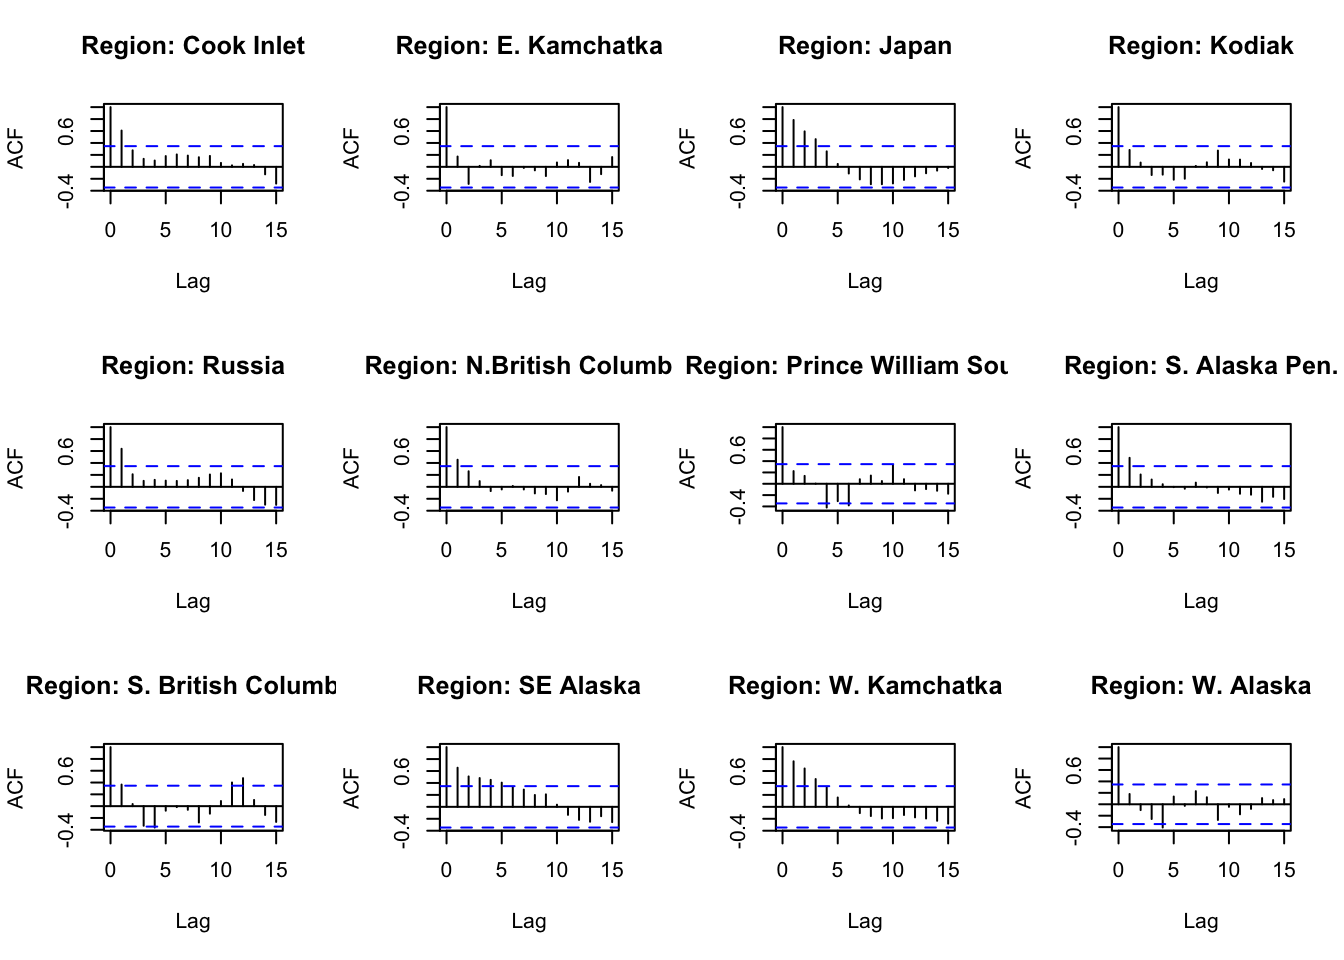
\includegraphics{Lab-1-Emma-ZR-MHS-draft_files/figure-latex/unnamed-chunk-43-1.pdf}

\begin{Shaded}
\begin{Highlighting}[]
\CommentTok{\#PACF plots for each region}
\FunctionTok{par}\NormalTok{(}\AttributeTok{mfrow=}\FunctionTok{c}\NormalTok{(}\DecValTok{3}\NormalTok{,}\DecValTok{4}\NormalTok{))}
\ControlFlowTok{for}\NormalTok{(r }\ControlFlowTok{in} \DecValTok{1}\SpecialCharTok{:}\FunctionTok{length}\NormalTok{(regions))\{}
  \FunctionTok{plot}\NormalTok{(DiagPlots\_even[[r]][[}\DecValTok{2}\NormalTok{]], }\AttributeTok{main =} \FunctionTok{paste0}\NormalTok{(}\StringTok{"Region: "}\NormalTok{, regionskey[r]))}
\NormalTok{\}}
\end{Highlighting}
\end{Shaded}

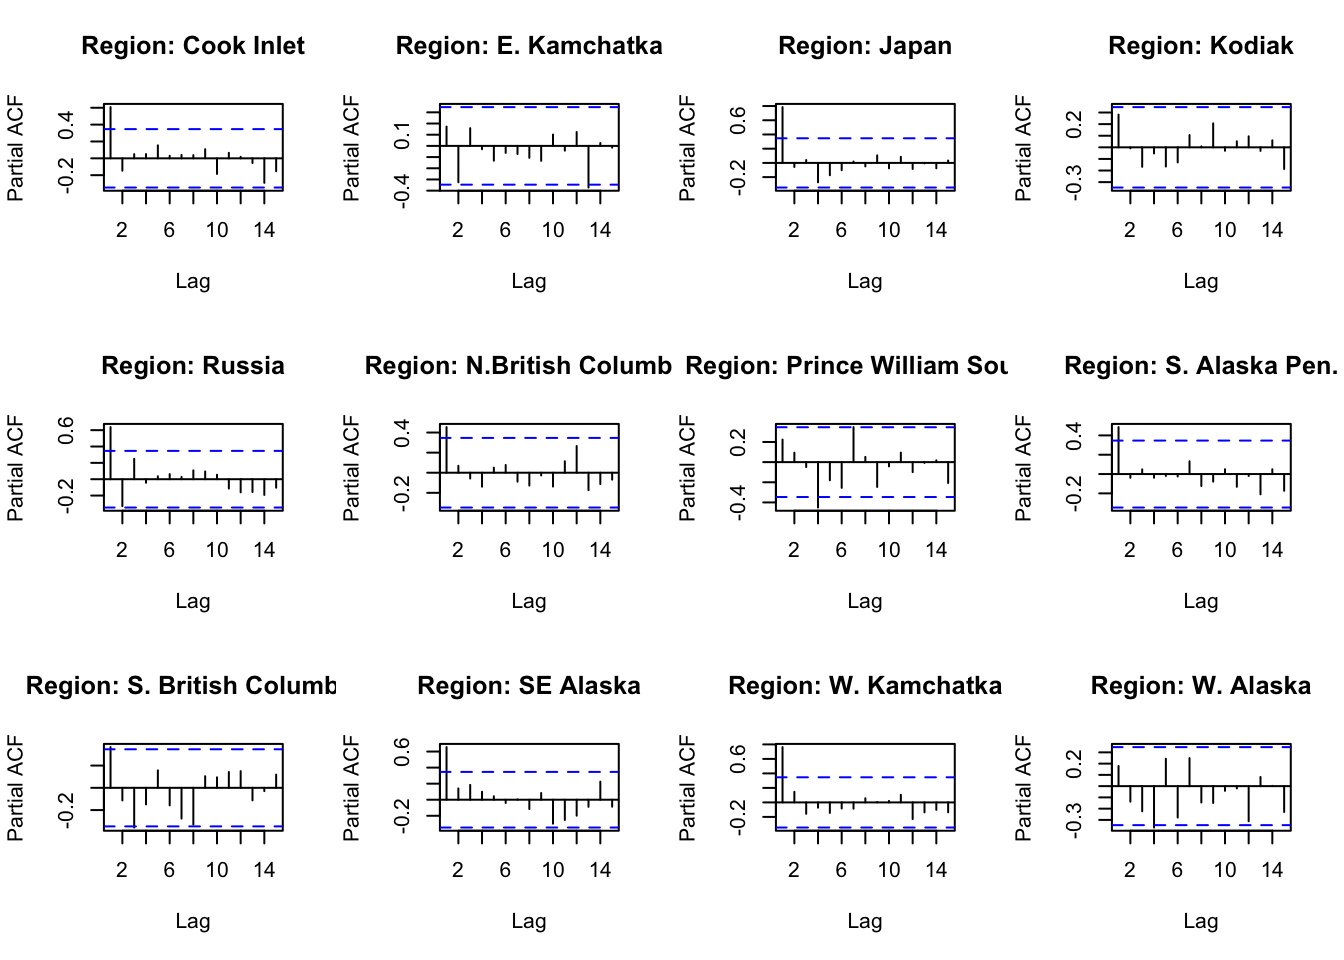
\includegraphics{Lab-1-Emma-ZR-MHS-draft_files/figure-latex/unnamed-chunk-43-2.pdf}
And then for odd years:

\begin{Shaded}
\begin{Highlighting}[]
\CommentTok{\#Odd Years }
\FunctionTok{par}\NormalTok{(}\AttributeTok{mfrow=}\FunctionTok{c}\NormalTok{(}\DecValTok{3}\NormalTok{,}\DecValTok{4}\NormalTok{))}
\ControlFlowTok{for}\NormalTok{(r }\ControlFlowTok{in} \DecValTok{1}\SpecialCharTok{:}\FunctionTok{length}\NormalTok{(regions))\{}
  \FunctionTok{plot}\NormalTok{(DiagPlots\_odd[[r]][[}\DecValTok{1}\NormalTok{]], }\AttributeTok{main =} \FunctionTok{paste0}\NormalTok{(}\StringTok{"Region: "}\NormalTok{, regionskey[r]))}
\NormalTok{\}}
\end{Highlighting}
\end{Shaded}

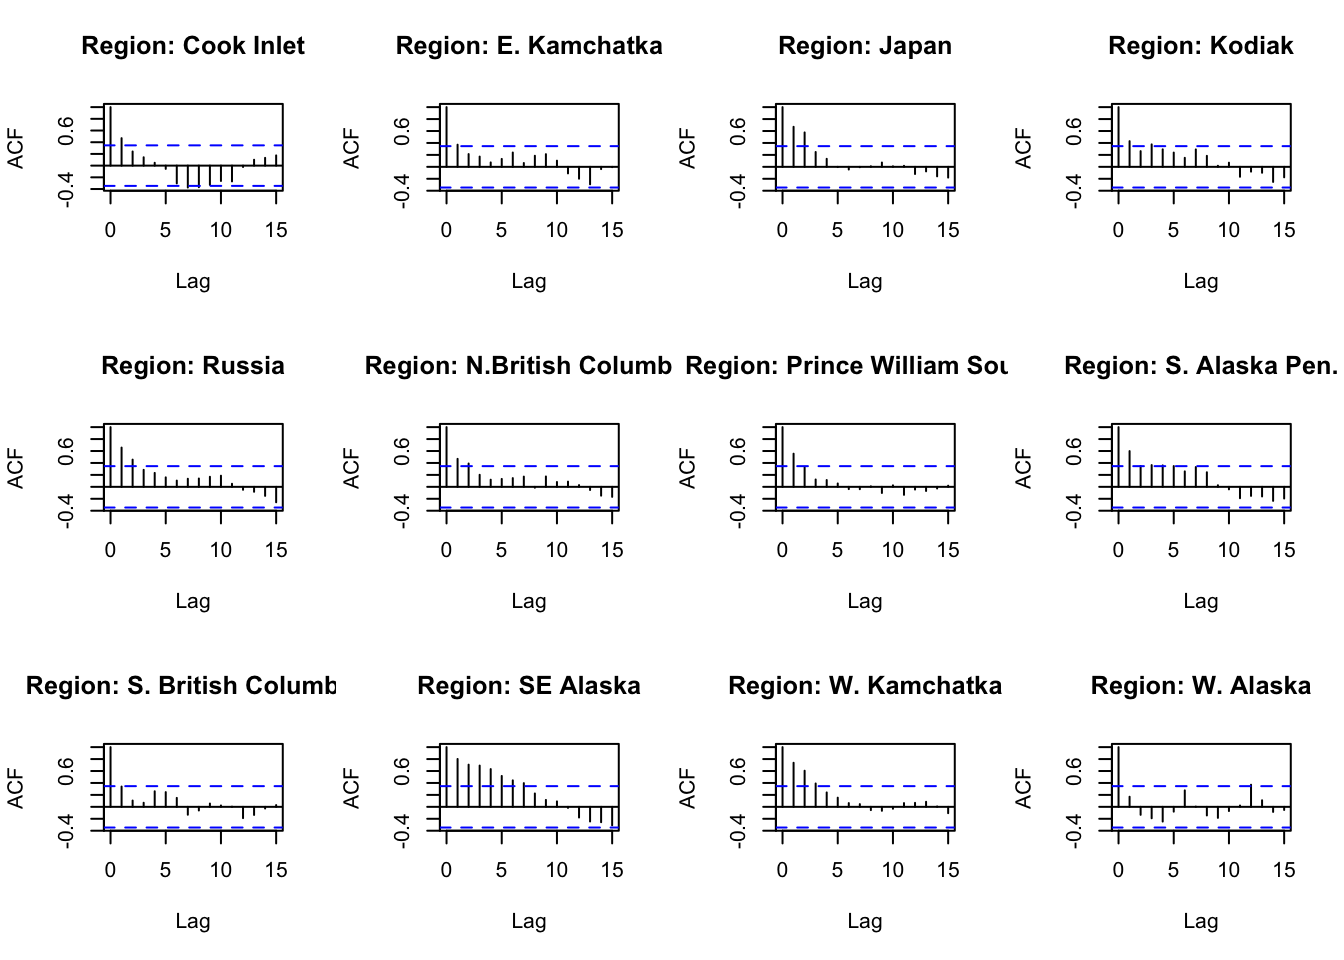
\includegraphics{Lab-1-Emma-ZR-MHS-draft_files/figure-latex/unnamed-chunk-44-1.pdf}

\begin{Shaded}
\begin{Highlighting}[]
\CommentTok{\#PACF plots for each region}
\FunctionTok{par}\NormalTok{(}\AttributeTok{mfrow=}\FunctionTok{c}\NormalTok{(}\DecValTok{3}\NormalTok{,}\DecValTok{4}\NormalTok{))}
\ControlFlowTok{for}\NormalTok{(r }\ControlFlowTok{in} \DecValTok{1}\SpecialCharTok{:}\FunctionTok{length}\NormalTok{(regions))\{}
  \FunctionTok{plot}\NormalTok{(DiagPlots\_odd[[r]][[}\DecValTok{2}\NormalTok{]], }\AttributeTok{main =} \FunctionTok{paste0}\NormalTok{(}\StringTok{"Region: "}\NormalTok{, regionskey[r]))}
\NormalTok{\}}
\end{Highlighting}
\end{Shaded}

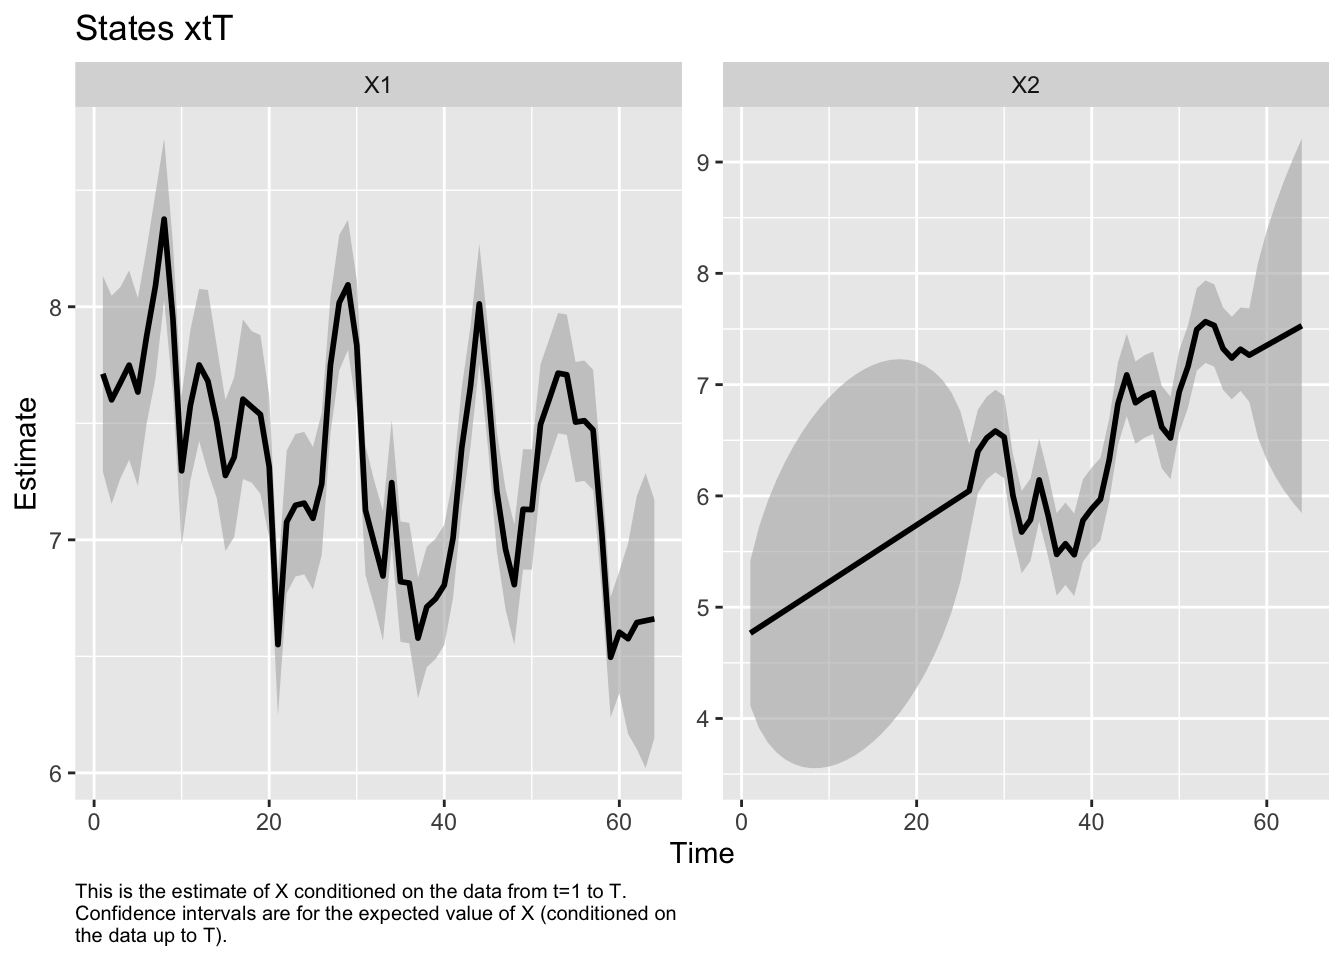
\includegraphics{Lab-1-Emma-ZR-MHS-draft_files/figure-latex/unnamed-chunk-44-2.pdf}

The next step is to look at the ARIMA models for regions by all years,
even and odd years, and define forecast levels. Let's start with all
years.

\begin{Shaded}
\begin{Highlighting}[]
\CommentTok{\#forecast levels}
\NormalTok{forecastlevels}\OtherTok{\textless{}{-}}\FunctionTok{c}\NormalTok{(}\DecValTok{5}\NormalTok{, }\DecValTok{10}\NormalTok{, }\DecValTok{20}\NormalTok{)}
\CommentTok{\#all combinations}
\NormalTok{Allcombs}\OtherTok{\textless{}{-}}\FunctionTok{expand\_grid}\NormalTok{(regions, forecastlevels)}

\CommentTok{\#================================================}

\CommentTok{\#All}
\NormalTok{RegionMods}\OtherTok{\textless{}{-}}\FunctionTok{mapply}\NormalTok{(FitModFunction, Allcombs}\SpecialCharTok{$}\NormalTok{regions, Allcombs}\SpecialCharTok{$}\NormalTok{forecastlevels, }\AttributeTok{SIMPLIFY =} \ConstantTok{FALSE}\NormalTok{)}
\CommentTok{\# head(RegionMods\_even)}
\CommentTok{\# names(RegionMods\_even)}
\end{Highlighting}
\end{Shaded}

Now let's consider even years.

\begin{Shaded}
\begin{Highlighting}[]
\CommentTok{\#Even}
\NormalTok{RegionMods\_even}\OtherTok{\textless{}{-}}\FunctionTok{mapply}\NormalTok{(FitModFunction\_even, Allcombs}\SpecialCharTok{$}\NormalTok{regions, Allcombs}\SpecialCharTok{$}\NormalTok{forecastlevels, }\AttributeTok{SIMPLIFY =} \ConstantTok{FALSE}\NormalTok{)}
\FunctionTok{head}\NormalTok{(RegionMods\_even)}
\end{Highlighting}
\end{Shaded}

\begin{verbatim}
## $ci
## $ci$Fit
## Series: train 
## ARIMA(0,1,0) 
## 
## sigma^2 = 0.3224:  log likelihood = -23.88
## AIC=49.77   AICc=49.92   BIC=51.1
## 
## $ci$MASE
## [1] 0.3602762
## 
## $ci$Bm
##                                  V1        V2      AIC DeltaAIC     Mod npar
## 1  ARIMA(0,1,0)                      55.48062 55.48062        0 0, 1, 0    0
## 
## 
## $ci
## $ci$Fit
## Series: train 
## ARIMA(0,1,0) 
## 
## sigma^2 = 0.3052:  log likelihood = -21.47
## AIC=44.93   AICc=45.1   BIC=46.19
## 
## $ci$MASE
## [1] 1.243461
## 
## $ci$Bm
##                                  V1        V2      AIC DeltaAIC     Mod npar
## 1  ARIMA(0,1,0)                      55.48062 55.48062        0 0, 1, 0    0
## 
## 
## $ci
## $ci$Fit
## Series: train 
## ARIMA(0,1,0) 
## 
## sigma^2 = 0.2563:  log likelihood = -15.5
## AIC=33.01   AICc=33.22   BIC=34.05
## 
## $ci$MASE
## [1] 0.3950404
## 
## $ci$Bm
##                                  V1        V2      AIC DeltaAIC     Mod npar
## 1  ARIMA(0,1,0)                      55.48062 55.48062        0 0, 1, 0    0
## 
## 
## $e_kam
## $e_kam$Fit
## Series: train 
## ARIMA(0,0,0) with non-zero mean 
## 
## Coefficients:
##         mean
##       2.6102
## s.e.  0.1257
## 
## sigma^2 = 0.4743:  log likelihood = -29.83
## AIC=63.65   AICc=64.11   BIC=66.39
## 
## $e_kam$MASE
## [1] 0.2398603
## 
## $e_kam$Bm
##                                  V1        V2      AIC DeltaAIC     Mod npar
## 1  ARIMA(0,0,0) with non-zero mean   71.15545 71.15545  0.43946 0, 0, 0    0
## 2  ARIMA(1,0,0) with non-zero mean   72.55604 72.55604  1.84005 1, 0, 0    1
## 3  ARIMA(0,0,1) with non-zero mean   70.71599 70.71599  0.00000 0, 0, 1    1
## 4  ARIMA(1,0,1) with non-zero mean   72.39343 72.39343  1.67744 1, 0, 1    2
## 5  ARIMA(0,0,2) with non-zero mean   71.53128 71.53128  0.81529 0, 0, 2    2
## 
## 
## $e_kam
## $e_kam$Fit
## Series: train 
## ARIMA(0,0,0) with non-zero mean 
## 
## Coefficients:
##         mean
##       2.5867
## s.e.  0.1318
## 
## sigma^2 = 0.4873:  log likelihood = -28.1
## AIC=60.19   AICc=60.69   BIC=62.79
## 
## $e_kam$MASE
## [1] 0.219349
## 
## $e_kam$Bm
##                                  V1        V2      AIC DeltaAIC     Mod npar
## 1  ARIMA(0,0,0) with non-zero mean   71.15545 71.15545  0.43946 0, 0, 0    0
## 2  ARIMA(1,0,0) with non-zero mean   72.55604 72.55604  1.84005 1, 0, 0    1
## 3  ARIMA(0,0,1) with non-zero mean   70.71599 70.71599  0.00000 0, 0, 1    1
## 4  ARIMA(1,0,1) with non-zero mean   72.39343 72.39343  1.67744 1, 0, 1    2
## 5  ARIMA(0,0,2) with non-zero mean   71.53128 71.53128  0.81529 0, 0, 2    2
## 
## 
## $e_kam
## $e_kam$Fit
## Series: train 
## ARIMA(0,0,0) with non-zero mean 
## 
## Coefficients:
##         mean
##       2.6917
## s.e.  0.1209
## 
## sigma^2 = 0.337:  log likelihood = -18.74
## AIC=41.48   AICc=42.12   BIC=43.67
## 
## $e_kam$MASE
## [1] 0.2382605
## 
## $e_kam$Bm
##                                  V1        V2      AIC DeltaAIC     Mod npar
## 1  ARIMA(0,0,0) with non-zero mean   71.15545 71.15545  0.43946 0, 0, 0    0
## 2  ARIMA(1,0,0) with non-zero mean   72.55604 72.55604  1.84005 1, 0, 0    1
## 3  ARIMA(0,0,1) with non-zero mean   70.71599 70.71599  0.00000 0, 0, 1    1
## 4  ARIMA(1,0,1) with non-zero mean   72.39343 72.39343  1.67744 1, 0, 1    2
## 5  ARIMA(0,0,2) with non-zero mean   71.53128 71.53128  0.81529 0, 0, 2    2
\end{verbatim}

\begin{Shaded}
\begin{Highlighting}[]
\CommentTok{\#names(RegionMods\_even) \#should be three for each region}
\end{Highlighting}
\end{Shaded}

Now let's consider odd years.

\begin{Shaded}
\begin{Highlighting}[]
\CommentTok{\#Odd }
\NormalTok{RegionMods\_odd}\OtherTok{\textless{}{-}}\FunctionTok{mapply}\NormalTok{(FitModFunction\_odd, Allcombs}\SpecialCharTok{$}\NormalTok{regions, Allcombs}\SpecialCharTok{$}\NormalTok{forecastlevels, }\AttributeTok{SIMPLIFY =} \ConstantTok{FALSE}\NormalTok{)}
\FunctionTok{head}\NormalTok{(RegionMods\_odd)}
\end{Highlighting}
\end{Shaded}

\begin{verbatim}
## $ci
## $ci$Fit
## Series: train 
## ARIMA(1,0,0) with zero mean 
## 
## Coefficients:
##          ar1
##       0.6039
## s.e.  0.1467
## 
## sigma^2 = 0.4057:  log likelihood = -27.79
## AIC=59.57   AICc=60.03   BIC=62.31
## 
## $ci$MASE
## [1] 2.144842
## 
## $ci$Bm
##                                  V1        V2      AIC DeltaAIC     Mod npar
## 1  ARIMA(1,0,0) with non-zero mean    75.3159 75.31590  0.36364 1, 0, 0    1
## 2  ARIMA(1,0,0) with zero mean       74.95226 74.95226  0.00000 1, 0, 0    1
## 
## 
## $ci
## $ci$Fit
## Series: train 
## ARIMA(1,0,0) with zero mean 
## 
## Coefficients:
##          ar1
##       0.6037
## s.e.  0.1610
## 
## sigma^2 = 0.4189:  log likelihood = -26.28
## AIC=56.57   AICc=57.07   BIC=59.16
## 
## $ci$MASE
## [1] 1.555645
## 
## $ci$Bm
##                                  V1        V2      AIC DeltaAIC     Mod npar
## 1  ARIMA(1,0,0) with non-zero mean    75.3159 75.31590  0.36364 1, 0, 0    1
## 2  ARIMA(1,0,0) with zero mean       74.95226 74.95226  0.00000 1, 0, 0    1
## 
## 
## $ci
## $ci$Fit
## Series: train 
## ARIMA(1,0,0) with zero mean 
## 
## Coefficients:
##          ar1
##       0.6430
## s.e.  0.1528
## 
## sigma^2 = 0.3645:  log likelihood = -19.87
## AIC=43.74   AICc=44.37   BIC=45.93
## 
## $ci$MASE
## [1] 1.425649
## 
## $ci$Bm
##                                  V1        V2      AIC DeltaAIC     Mod npar
## 1  ARIMA(1,0,0) with non-zero mean    75.3159 75.31590  0.36364 1, 0, 0    1
## 2  ARIMA(1,0,0) with zero mean       74.95226 74.95226  0.00000 1, 0, 0    1
## 
## 
## $e_kam
## $e_kam$Fit
## Series: train 
## ARIMA(0,1,0) 
## 
## sigma^2 = 0.1936:  log likelihood = -16.75
## AIC=35.49   AICc=35.65   BIC=36.82
## 
## $e_kam$MASE
## [1] 0.1721234
## 
## $e_kam$Bm
##                                  V1        V2      AIC DeltaAIC     Mod npar
## 1  ARIMA(1,1,0) with drift           60.55848 60.55848  1.02617 1, 1, 0    2
## 2  ARIMA(0,1,0)                      59.53231 59.53231  0.00000 0, 1, 0    0
## 
## 
## $e_kam
## $e_kam$Fit
## Series: train 
## ARIMA(0,0,1) with non-zero mean 
## 
## Coefficients:
##          ma1    mean
##       0.5514  3.9961
## s.e.  0.1250  0.1117
## 
## sigma^2 = 0.1551:  log likelihood = -12.29
## AIC=30.59   AICc=31.63   BIC=34.48
## 
## $e_kam$MASE
## [1] 0.2364036
## 
## $e_kam$Bm
##                                  V1        V2      AIC DeltaAIC     Mod npar
## 1  ARIMA(1,1,0) with drift           60.55848 60.55848  1.02617 1, 1, 0    2
## 2  ARIMA(0,1,0)                      59.53231 59.53231  0.00000 0, 1, 0    0
## 
## 
## $e_kam
## $e_kam$Fit
## Series: train 
## ARIMA(0,0,1) with non-zero mean 
## 
## Coefficients:
##          ma1    mean
##       0.5404  3.9140
## s.e.  0.1481  0.1168
## 
## sigma^2 = 0.1433:  log likelihood = -8.97
## AIC=23.94   AICc=25.28   BIC=27.21
## 
## $e_kam$MASE
## [1] 0.1918676
## 
## $e_kam$Bm
##                                  V1        V2      AIC DeltaAIC     Mod npar
## 1  ARIMA(1,1,0) with drift           60.55848 60.55848  1.02617 1, 1, 0    2
## 2  ARIMA(0,1,0)                      59.53231 59.53231  0.00000 0, 1, 0    0
\end{verbatim}

\begin{Shaded}
\begin{Highlighting}[]
\CommentTok{\#names(RegionMods\_odd) \#should be three for each region}
\end{Highlighting}
\end{Shaded}

Now, we're extracting the MASE and creating our final model tables

\begin{Shaded}
\begin{Highlighting}[]
\CommentTok{\#getting MASE}
\CommentTok{\#All}
\NormalTok{RegionMASE}\OtherTok{\textless{}{-}}\FunctionTok{sapply}\NormalTok{(RegionMods, }\ControlFlowTok{function}\NormalTok{(x)\{y}\OtherTok{\textless{}{-}}\NormalTok{x}\SpecialCharTok{$}\NormalTok{MASE\})}
\NormalTok{RegionBestMod}\OtherTok{\textless{}{-}}\FunctionTok{sapply}\NormalTok{(RegionMods, }\ControlFlowTok{function}\NormalTok{(x)\{y}\OtherTok{\textless{}{-}}\FunctionTok{as.character}\NormalTok{(x}\SpecialCharTok{$}\NormalTok{Fit)\})}
\CommentTok{\#Even}
\NormalTok{RegionMASE\_even}\OtherTok{\textless{}{-}}\FunctionTok{sapply}\NormalTok{(RegionMods\_even, }\ControlFlowTok{function}\NormalTok{(x)\{y}\OtherTok{\textless{}{-}}\NormalTok{x}\SpecialCharTok{$}\NormalTok{MASE\})}
\NormalTok{RegionBestMod\_even}\OtherTok{\textless{}{-}}\FunctionTok{sapply}\NormalTok{(RegionMods\_even, }\ControlFlowTok{function}\NormalTok{(x)\{y}\OtherTok{\textless{}{-}}\FunctionTok{as.character}\NormalTok{(x}\SpecialCharTok{$}\NormalTok{Fit)\})}
\CommentTok{\#Odd}
\NormalTok{RegionMASE\_odd}\OtherTok{\textless{}{-}}\FunctionTok{sapply}\NormalTok{(RegionMods\_odd, }\ControlFlowTok{function}\NormalTok{(x)\{y}\OtherTok{\textless{}{-}}\NormalTok{x}\SpecialCharTok{$}\NormalTok{MASE\})}
\NormalTok{RegionBestMod\_odd}\OtherTok{\textless{}{-}}\FunctionTok{sapply}\NormalTok{(RegionMods\_odd, }\ControlFlowTok{function}\NormalTok{(x)\{y}\OtherTok{\textless{}{-}}\FunctionTok{as.character}\NormalTok{(x}\SpecialCharTok{$}\NormalTok{Fit)\})}
\CommentTok{\#combine into tables}
\CommentTok{\#all}
\NormalTok{ResultsTable}\OtherTok{\textless{}{-}}\NormalTok{Allcombs }\SpecialCharTok{\%\textgreater{}\%} \FunctionTok{add\_column}\NormalTok{(}\AttributeTok{Model =}\NormalTok{ RegionBestMod, }\AttributeTok{MASE =}\NormalTok{ RegionMASE)}
\NormalTok{ResultsTable}
\end{Highlighting}
\end{Shaded}

\begin{verbatim}
## # A tibble: 36 x 4
##    regions forecastlevels Model                            MASE
##    <chr>            <dbl> <chr>                           <dbl>
##  1 ci                   5 ARIMA(2,0,0) with non-zero mean 0.460
##  2 ci                  10 ARIMA(2,0,0) with non-zero mean 0.549
##  3 ci                  20 ARIMA(1,0,1) with non-zero mean 0.711
##  4 e_kam                5 ARIMA(2,0,0) with non-zero mean 0.134
##  5 e_kam               10 ARIMA(2,0,0) with non-zero mean 0.111
##  6 e_kam               20 ARIMA(2,0,0) with non-zero mean 0.196
##  7 japan                5 ARIMA(0,0,0) with non-zero mean 0.744
##  8 japan               10 ARIMA(0,0,0) with non-zero mean 0.901
##  9 japan               20 ARIMA(0,1,1)                    0.853
## 10 kod                  5 ARIMA(0,1,1) with drift         0.221
## # i 26 more rows
\end{verbatim}

\begin{Shaded}
\begin{Highlighting}[]
\CommentTok{\#even}
\NormalTok{ResultsTable\_even}\OtherTok{\textless{}{-}}\NormalTok{Allcombs }\SpecialCharTok{\%\textgreater{}\%} \FunctionTok{add\_column}\NormalTok{(}\AttributeTok{Model =}\NormalTok{ RegionBestMod\_even, }\AttributeTok{MASE =}\NormalTok{ RegionMASE\_even)}
\NormalTok{ResultsTable\_even}
\end{Highlighting}
\end{Shaded}

\begin{verbatim}
## # A tibble: 36 x 4
##    regions forecastlevels Model                            MASE
##    <chr>            <dbl> <chr>                           <dbl>
##  1 ci                   5 ARIMA(0,1,0)                    0.360
##  2 ci                  10 ARIMA(0,1,0)                    1.24 
##  3 ci                  20 ARIMA(0,1,0)                    0.395
##  4 e_kam                5 ARIMA(0,0,0) with non-zero mean 0.240
##  5 e_kam               10 ARIMA(0,0,0) with non-zero mean 0.219
##  6 e_kam               20 ARIMA(0,0,0) with non-zero mean 0.238
##  7 japan                5 ARIMA(0,1,0)                    0.743
##  8 japan               10 ARIMA(0,1,0)                    0.500
##  9 japan               20 ARIMA(1,0,0) with non-zero mean 0.731
## 10 kod                  5 ARIMA(0,0,0) with non-zero mean 0.155
## # i 26 more rows
\end{verbatim}

\begin{Shaded}
\begin{Highlighting}[]
\CommentTok{\#Odd}
\NormalTok{ResultsTable\_odd}\OtherTok{\textless{}{-}}\NormalTok{Allcombs }\SpecialCharTok{\%\textgreater{}\%} \FunctionTok{add\_column}\NormalTok{(}\AttributeTok{Model =}\NormalTok{ RegionBestMod\_odd, }\AttributeTok{MASE =}\NormalTok{ RegionMASE\_odd)}
\NormalTok{ResultsTable\_odd}
\end{Highlighting}
\end{Shaded}

\begin{verbatim}
## # A tibble: 36 x 4
##    regions forecastlevels Model                            MASE
##    <chr>            <dbl> <chr>                           <dbl>
##  1 ci                   5 ARIMA(1,0,0) with zero mean     2.14 
##  2 ci                  10 ARIMA(1,0,0) with zero mean     1.56 
##  3 ci                  20 ARIMA(1,0,0) with zero mean     1.43 
##  4 e_kam                5 ARIMA(0,1,0)                    0.172
##  5 e_kam               10 ARIMA(0,0,1) with non-zero mean 0.236
##  6 e_kam               20 ARIMA(0,0,1) with non-zero mean 0.192
##  7 japan                5 ARIMA(1,1,0)                    0.898
##  8 japan               10 ARIMA(0,1,0)                    0.557
##  9 japan               20 ARIMA(1,0,0) with non-zero mean 0.550
## 10 kod                  5 ARIMA(0,1,0)                    0.124
## # i 26 more rows
\end{verbatim}

\hypertarget{results}{%
\section{Results}\label{results}}

\hypertarget{sockeye}{%
\subsection{Sockeye:}\label{sockeye}}

Plot MASE for three different forecast periods - 5, 10, and 20 years -
across all regions. MASE \textless{} 1 is a ``good'' value.

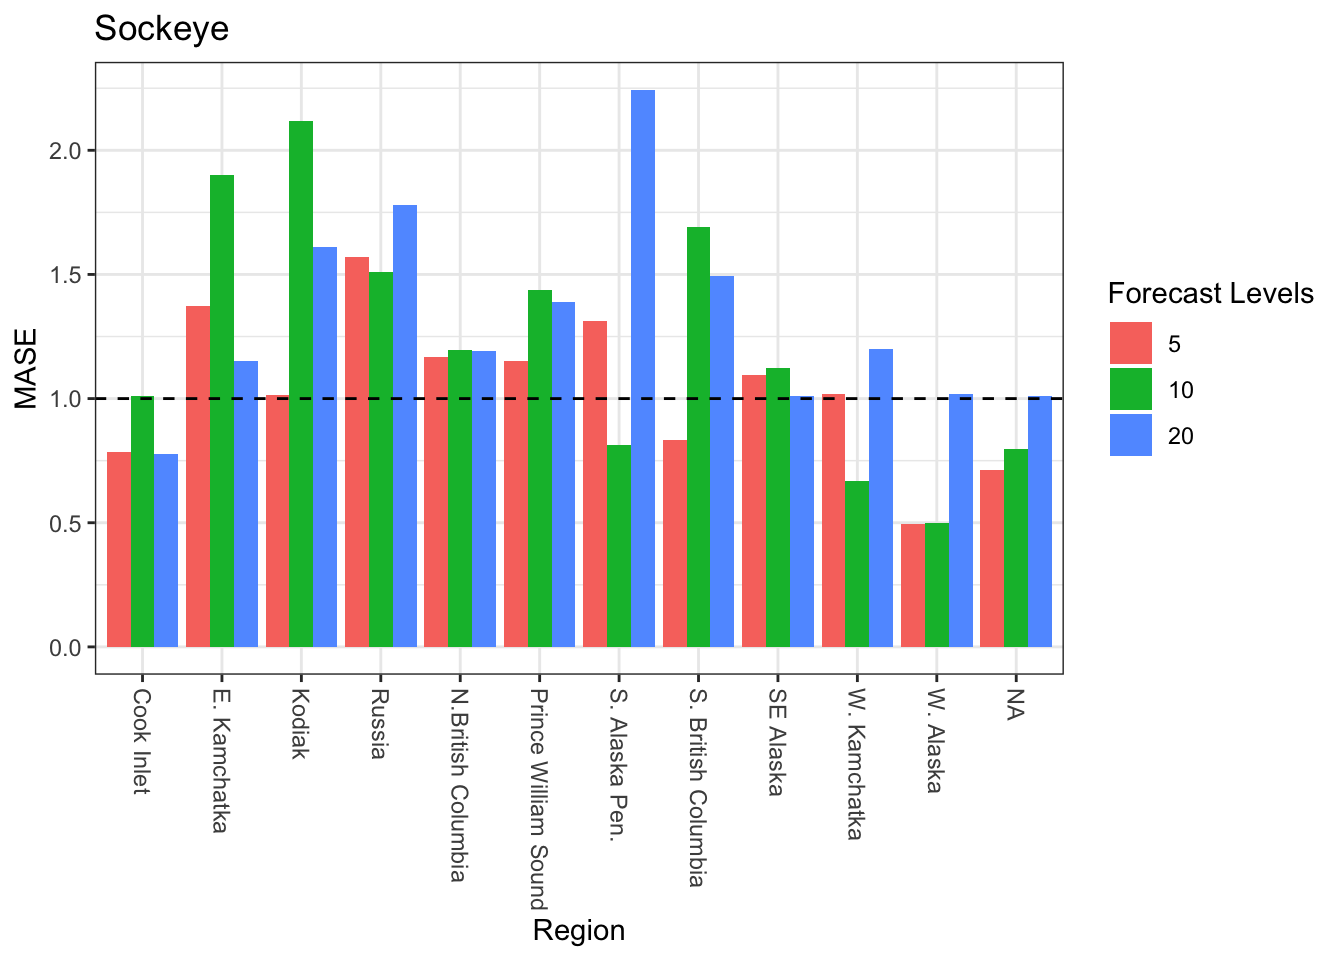
\includegraphics{Lab-1-Emma-ZR-MHS-draft_files/figure-latex/unnamed-chunk-49-1.pdf}

None of the ARIMA models performed well for the forecasts of 20 years of
data. Below is a comparison of the three lengths of forecasted data for
South British Columbia where MASE was below 1 for the 5 year forecast
but \textgreater1 for the 10 and 20 year forecasts.

\begin{Shaded}
\begin{Highlighting}[]
\NormalTok{sock.sbc}\OtherTok{\textless{}{-}}\FunctionTok{subset}\NormalTok{(SockByRegion, region}\SpecialCharTok{==}\StringTok{\textquotesingle{}sbc\textquotesingle{}}\NormalTok{)}
\NormalTok{sbc.ts}\OtherTok{\textless{}{-}}\FunctionTok{ts}\NormalTok{(sock.sbc}\SpecialCharTok{$}\NormalTok{lnreturns, }\AttributeTok{start=}\NormalTok{sock.sbc}\SpecialCharTok{$}\NormalTok{year[}\DecValTok{1}\NormalTok{])}
\CommentTok{\#create training and test datasets for the 5, 10, and 20 year forecasts}
\NormalTok{train.sbc5}\OtherTok{\textless{}{-}}\FunctionTok{window}\NormalTok{(sbc.ts, }\AttributeTok{start=}\DecValTok{1952}\NormalTok{, }\AttributeTok{end=}\DecValTok{2010}\NormalTok{)}
\NormalTok{test.sbc5}\OtherTok{\textless{}{-}}\FunctionTok{window}\NormalTok{(sbc.ts, }\AttributeTok{start=}\DecValTok{2011}\NormalTok{, }\AttributeTok{end=}\DecValTok{2015}\NormalTok{)}
\NormalTok{sbc.final5}\OtherTok{\textless{}{-}}\NormalTok{forecast}\SpecialCharTok{::}\FunctionTok{auto.arima}\NormalTok{(train.sbc5, }\AttributeTok{approximation =}\NormalTok{ F, }\AttributeTok{stepwise =}\NormalTok{ F)}

\NormalTok{train.sbc10}\OtherTok{\textless{}{-}}\FunctionTok{window}\NormalTok{(sbc.ts, }\AttributeTok{start=}\DecValTok{1952}\NormalTok{, }\AttributeTok{end=}\DecValTok{2005}\NormalTok{)}
\NormalTok{test.sbc10}\OtherTok{\textless{}{-}}\FunctionTok{window}\NormalTok{(sbc.ts, }\AttributeTok{start=}\DecValTok{2006}\NormalTok{, }\AttributeTok{end=}\DecValTok{2015}\NormalTok{)}
\NormalTok{sbc.final10}\OtherTok{\textless{}{-}}\NormalTok{forecast}\SpecialCharTok{::}\FunctionTok{auto.arima}\NormalTok{(train.sbc10, }\AttributeTok{approximation =}\NormalTok{ F, }\AttributeTok{stepwise =}\NormalTok{ F)}

\NormalTok{train.sbc20}\OtherTok{\textless{}{-}}\FunctionTok{window}\NormalTok{(sbc.ts, }\AttributeTok{start=}\DecValTok{1952}\NormalTok{, }\AttributeTok{end=}\DecValTok{1995}\NormalTok{)}
\NormalTok{test.sbc20}\OtherTok{\textless{}{-}}\FunctionTok{window}\NormalTok{(sbc.ts, }\AttributeTok{start=}\DecValTok{1996}\NormalTok{, }\AttributeTok{end=}\DecValTok{2015}\NormalTok{)}
\NormalTok{sbc.final20}\OtherTok{\textless{}{-}}\NormalTok{forecast}\SpecialCharTok{::}\FunctionTok{auto.arima}\NormalTok{(train.sbc20, }\AttributeTok{approximation =}\NormalTok{ F, }\AttributeTok{stepwise =}\NormalTok{ F)}
\end{Highlighting}
\end{Shaded}

Here are plots of the three forecast scenarios for sockeye in South
British Columbia.

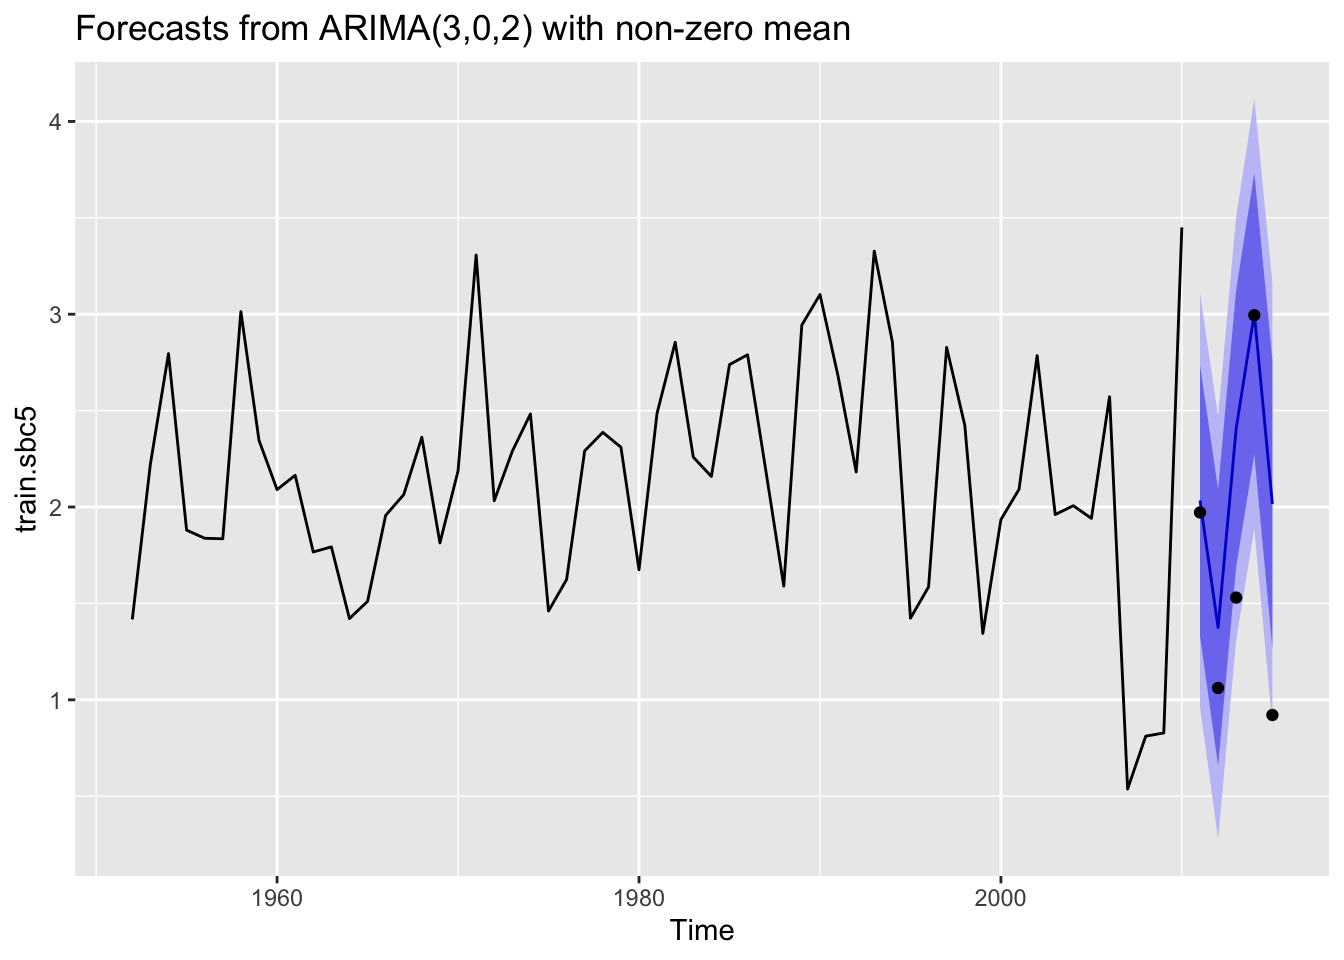
\includegraphics{Lab-1-Emma-ZR-MHS-draft_files/figure-latex/unnamed-chunk-51-1.pdf}
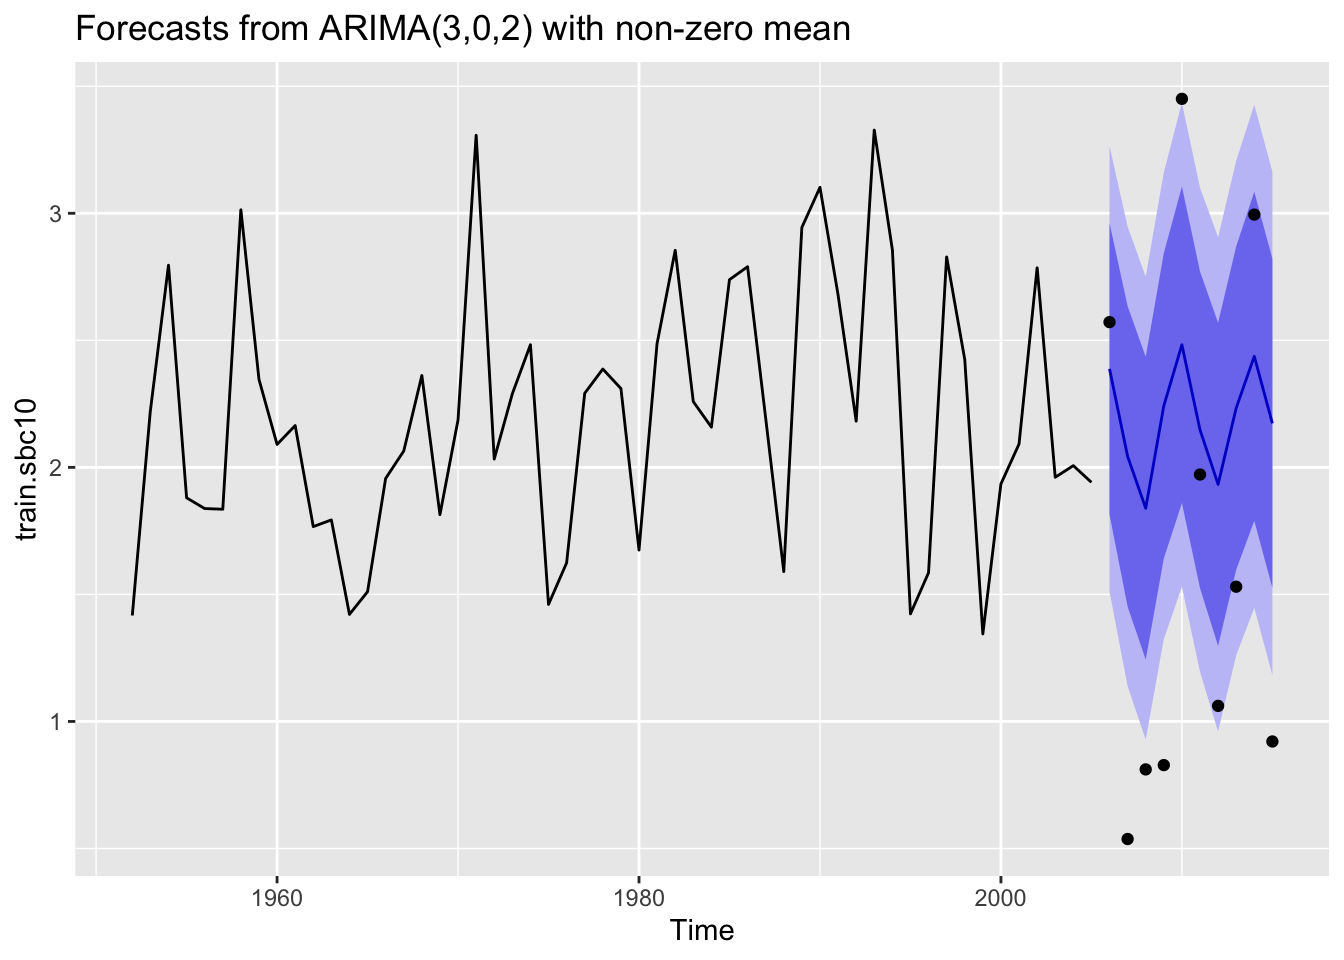
\includegraphics{Lab-1-Emma-ZR-MHS-draft_files/figure-latex/unnamed-chunk-51-2.pdf}
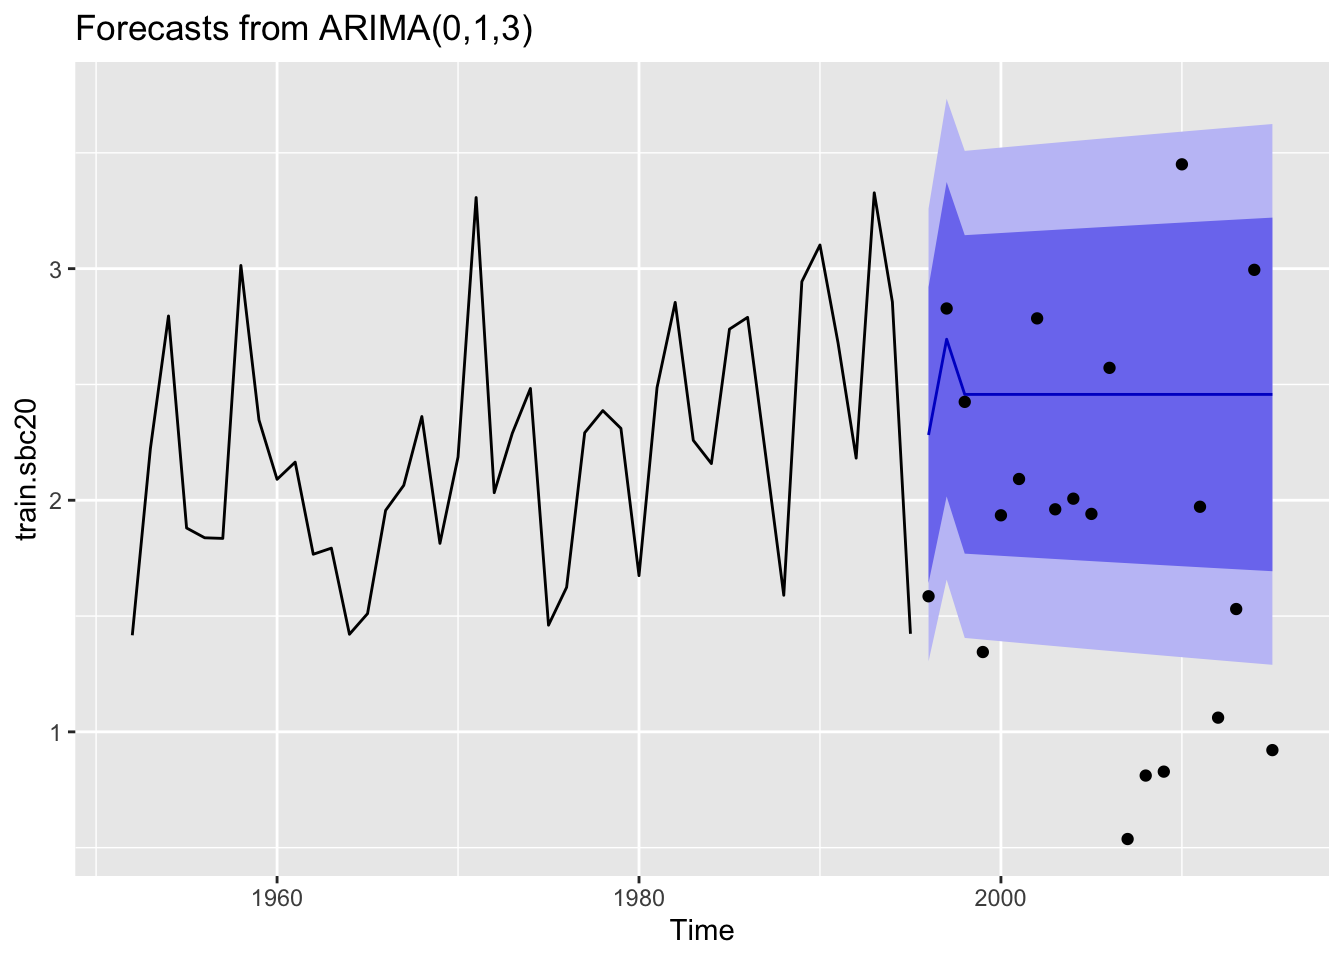
\includegraphics{Lab-1-Emma-ZR-MHS-draft_files/figure-latex/unnamed-chunk-51-3.pdf}

Looking at stationarity:

\begin{Shaded}
\begin{Highlighting}[]
\NormalTok{Ndiff}\OtherTok{\textless{}{-}}\FunctionTok{sapply}\NormalTok{(RegionBestModSock, }\ControlFlowTok{function}\NormalTok{(x)\{}
\NormalTok{  a}\OtherTok{\textless{}{-}}\FunctionTok{strsplit}\NormalTok{(}\FunctionTok{strsplit}\NormalTok{(}\FunctionTok{strsplit}\NormalTok{(x, }\StringTok{"[(]"}\NormalTok{)[[}\DecValTok{1}\NormalTok{]][}\DecValTok{2}\NormalTok{], }\StringTok{"[)]"}\NormalTok{)[[}\DecValTok{1}\NormalTok{]][}\DecValTok{1}\NormalTok{],}\StringTok{"[,]"}\NormalTok{)}
  \FunctionTok{return}\NormalTok{(a[[}\DecValTok{1}\NormalTok{]][}\DecValTok{2}\NormalTok{])\}}
\NormalTok{)}

\FunctionTok{tibble}\NormalTok{(}\AttributeTok{Ndiff =}\NormalTok{ Ndiff, }\AttributeTok{region =}\NormalTok{ Allcombs}\SpecialCharTok{$}\NormalTok{regions, }\AttributeTok{level =}\NormalTok{ Allcombs}\SpecialCharTok{$}\NormalTok{forecastlevels) }\SpecialCharTok{\%\textgreater{}\%}
  \FunctionTok{ggplot}\NormalTok{() }\SpecialCharTok{+} \FunctionTok{geom\_bar}\NormalTok{(}\FunctionTok{aes}\NormalTok{(}\AttributeTok{x =}\NormalTok{ region, }\AttributeTok{y =}\NormalTok{ Ndiff, }\AttributeTok{fill =} \FunctionTok{as.factor}\NormalTok{(level)), }\AttributeTok{stat =} \StringTok{"identity"}\NormalTok{, }\AttributeTok{position =} \StringTok{"dodge"}\NormalTok{) }\SpecialCharTok{+}
  \FunctionTok{scale\_x\_discrete}\NormalTok{(}\AttributeTok{labels =} \FunctionTok{as\_labeller}\NormalTok{(regionskey)) }\SpecialCharTok{+}
  \FunctionTok{labs}\NormalTok{(}\AttributeTok{fill =} \StringTok{"Forecast Levels"}\NormalTok{, }\AttributeTok{x =} \StringTok{"Region"}\NormalTok{, }\AttributeTok{y =} \StringTok{"Number of Differences"}\NormalTok{) }\SpecialCharTok{+} 
  \FunctionTok{ggtitle}\NormalTok{(}\StringTok{"Number of differences to achieve stationarity (Sockeye)"}\NormalTok{) }\SpecialCharTok{+} \FunctionTok{theme\_bw}\NormalTok{() }\SpecialCharTok{+} \FunctionTok{theme}\NormalTok{(}\AttributeTok{axis.text.x=}\FunctionTok{element\_text}\NormalTok{(}\AttributeTok{angle=}\SpecialCharTok{{-}}\DecValTok{90}\NormalTok{, }\AttributeTok{hjust =} \DecValTok{0}\NormalTok{, }\AttributeTok{vjust =} \FloatTok{0.5}\NormalTok{ ))}
\end{Highlighting}
\end{Shaded}

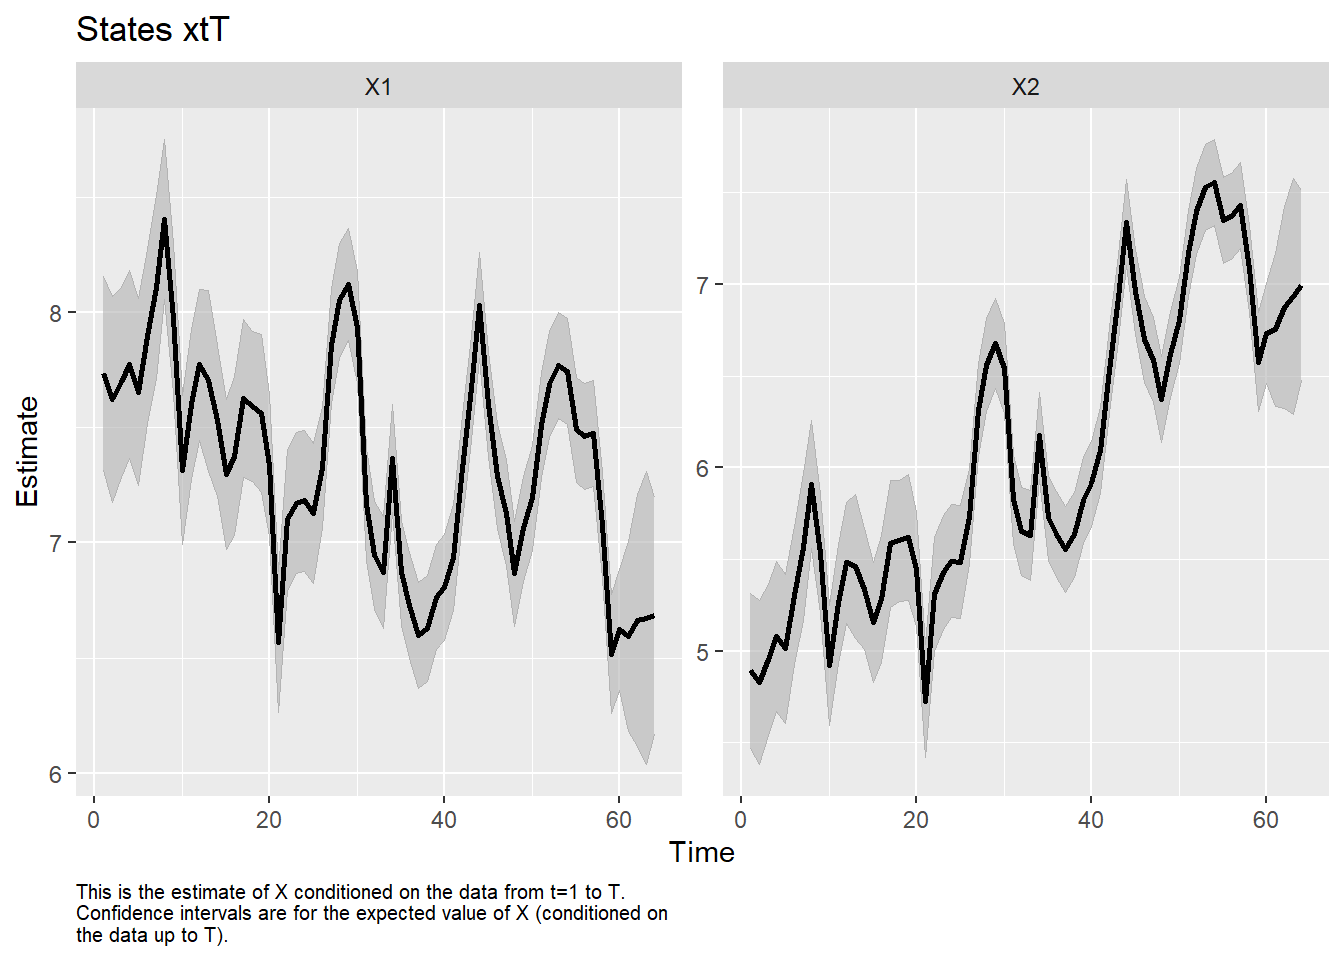
\includegraphics{Lab-1-Emma-ZR-MHS-draft_files/figure-latex/unnamed-chunk-52-1.pdf}
For Sockeye, 6 regions required differencing for all of the three
subsets of the data (3 forecasting levels). Two regions required
differencing for one subset of the data; four regions were stationary at
any level of subsetting.

None of the regional models for the 5-year forecast had autocorrelation
in the residuals based on the results of the Ljung-Box test (p-value
\textgreater{} 0.05).

\hypertarget{chum}{%
\subsection{Chum:}\label{chum}}

\begin{Shaded}
\begin{Highlighting}[]
\FunctionTok{ggplot}\NormalTok{(ResultsTableChum) }\SpecialCharTok{+} 
  \FunctionTok{geom\_bar}\NormalTok{(}\FunctionTok{aes}\NormalTok{(}\AttributeTok{x =}\NormalTok{ regions, }\AttributeTok{y =}\NormalTok{ MASE, }\AttributeTok{fill =} \FunctionTok{as.factor}\NormalTok{(forecastlevels)), }\AttributeTok{stat =} \StringTok{"identity"}\NormalTok{, }\AttributeTok{position =} \StringTok{"dodge"}\NormalTok{) }\SpecialCharTok{+} 
  \FunctionTok{geom\_hline}\NormalTok{(}\FunctionTok{aes}\NormalTok{(}\AttributeTok{yintercept =} \DecValTok{1}\NormalTok{), }\AttributeTok{linetype =} \StringTok{"dashed"}\NormalTok{) }\SpecialCharTok{+} 
  \FunctionTok{scale\_x\_discrete}\NormalTok{(}\AttributeTok{labels =} \FunctionTok{as\_labeller}\NormalTok{(regionskey)) }\SpecialCharTok{+}
  \FunctionTok{labs}\NormalTok{(}\AttributeTok{fill =} \StringTok{"Forecast Levels"}\NormalTok{, }\AttributeTok{x =} \StringTok{"Region"}\NormalTok{) }\SpecialCharTok{+} 
  \FunctionTok{ggtitle}\NormalTok{(}\StringTok{"Chum"}\NormalTok{) }\SpecialCharTok{+} \FunctionTok{theme\_bw}\NormalTok{() }\SpecialCharTok{+} \FunctionTok{theme}\NormalTok{(}\AttributeTok{axis.text.x=}\FunctionTok{element\_text}\NormalTok{(}\AttributeTok{angle=}\SpecialCharTok{{-}}\DecValTok{90}\NormalTok{, }\AttributeTok{hjust =} \DecValTok{0}\NormalTok{, }\AttributeTok{vjust =} \FloatTok{0.5}\NormalTok{ ))}
\end{Highlighting}
\end{Shaded}

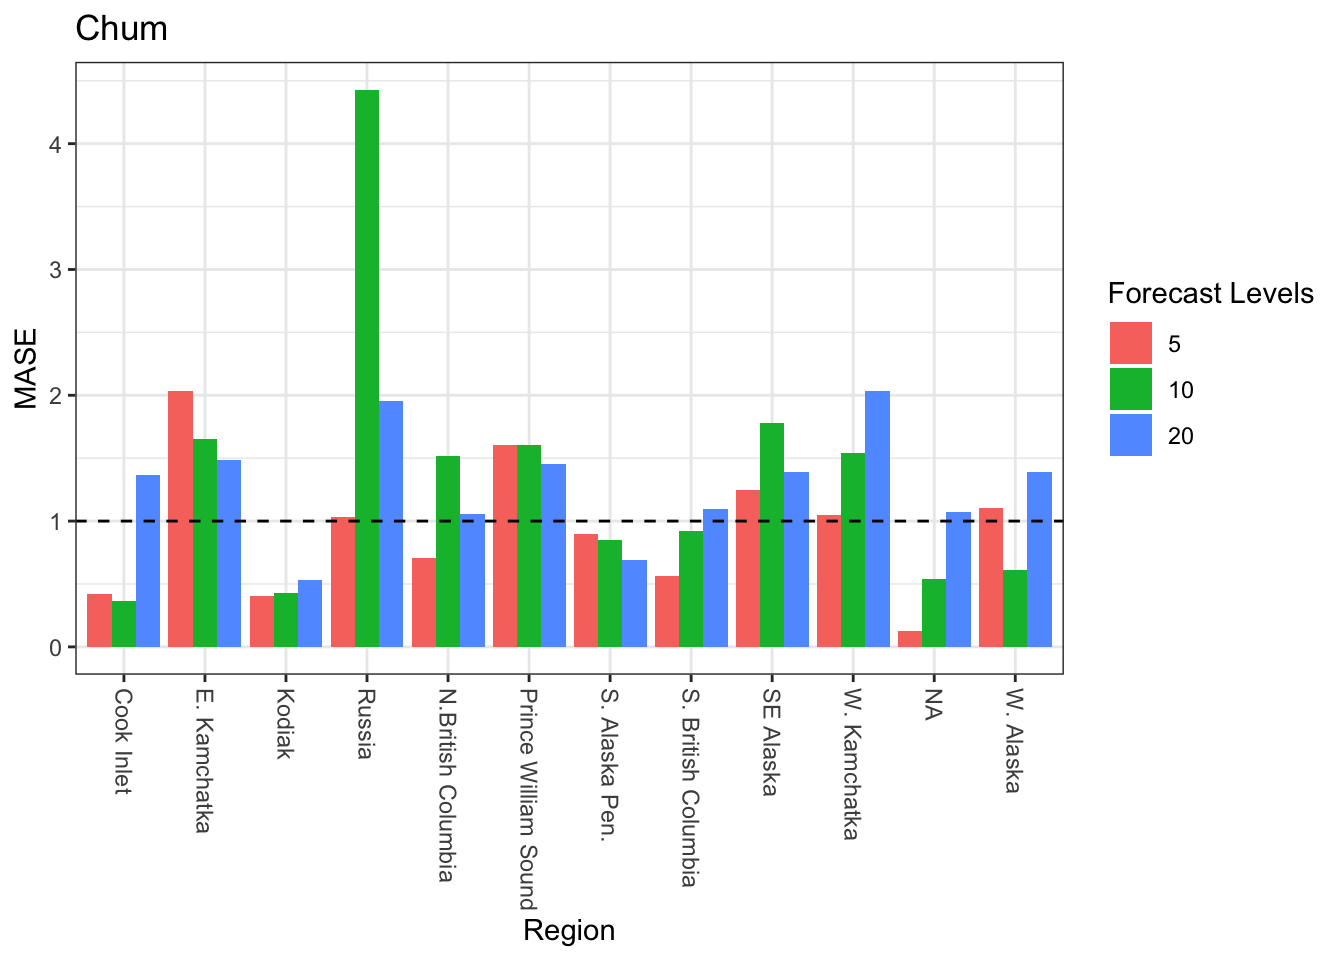
\includegraphics{Lab-1-Emma-ZR-MHS-draft_files/figure-latex/unnamed-chunk-53-1.pdf}

Many of the 5 and 10 year forecasts for Chum seem to perform well across
regions. Models fit to data in Russia do the worst at forecasting in
that region. Additionally, forecasts are poor across the different
numbers of years tested in E. Kamachatka, SE Alaska and W. Kamachatka.

20 year forecast for Kodiak:

\begin{Shaded}
\begin{Highlighting}[]
\NormalTok{chum.kod}\OtherTok{\textless{}{-}}\FunctionTok{subset}\NormalTok{(ChumByRegion, region}\SpecialCharTok{==}\StringTok{\textquotesingle{}kod\textquotesingle{}}\NormalTok{)}
\NormalTok{chum.ts}\OtherTok{\textless{}{-}}\FunctionTok{ts}\NormalTok{(chum.kod}\SpecialCharTok{$}\NormalTok{lnreturns, }\AttributeTok{start=}\NormalTok{chum.kod}\SpecialCharTok{$}\NormalTok{year[}\DecValTok{1}\NormalTok{])}
\CommentTok{\#test datasets for plotting}
\NormalTok{test.kod20}\OtherTok{\textless{}{-}}\FunctionTok{window}\NormalTok{(chum.ts, }\AttributeTok{start=}\DecValTok{1996}\NormalTok{, }\AttributeTok{end=}\DecValTok{2015}\NormalTok{)}
\FunctionTok{forecast}\NormalTok{(RegionModsChum[[}\DecValTok{9}\NormalTok{]]}\SpecialCharTok{$}\NormalTok{Fit, }\AttributeTok{h =} \DecValTok{20}\NormalTok{) }\SpecialCharTok{\%\textgreater{}\%} \FunctionTok{autoplot}\NormalTok{() }\SpecialCharTok{+} \FunctionTok{geom\_point}\NormalTok{(}\FunctionTok{aes}\NormalTok{(}\AttributeTok{x=}\NormalTok{x, }\AttributeTok{y=}\NormalTok{y), }\AttributeTok{data=}\FunctionTok{fortify}\NormalTok{(test.kod20))}
\end{Highlighting}
\end{Shaded}

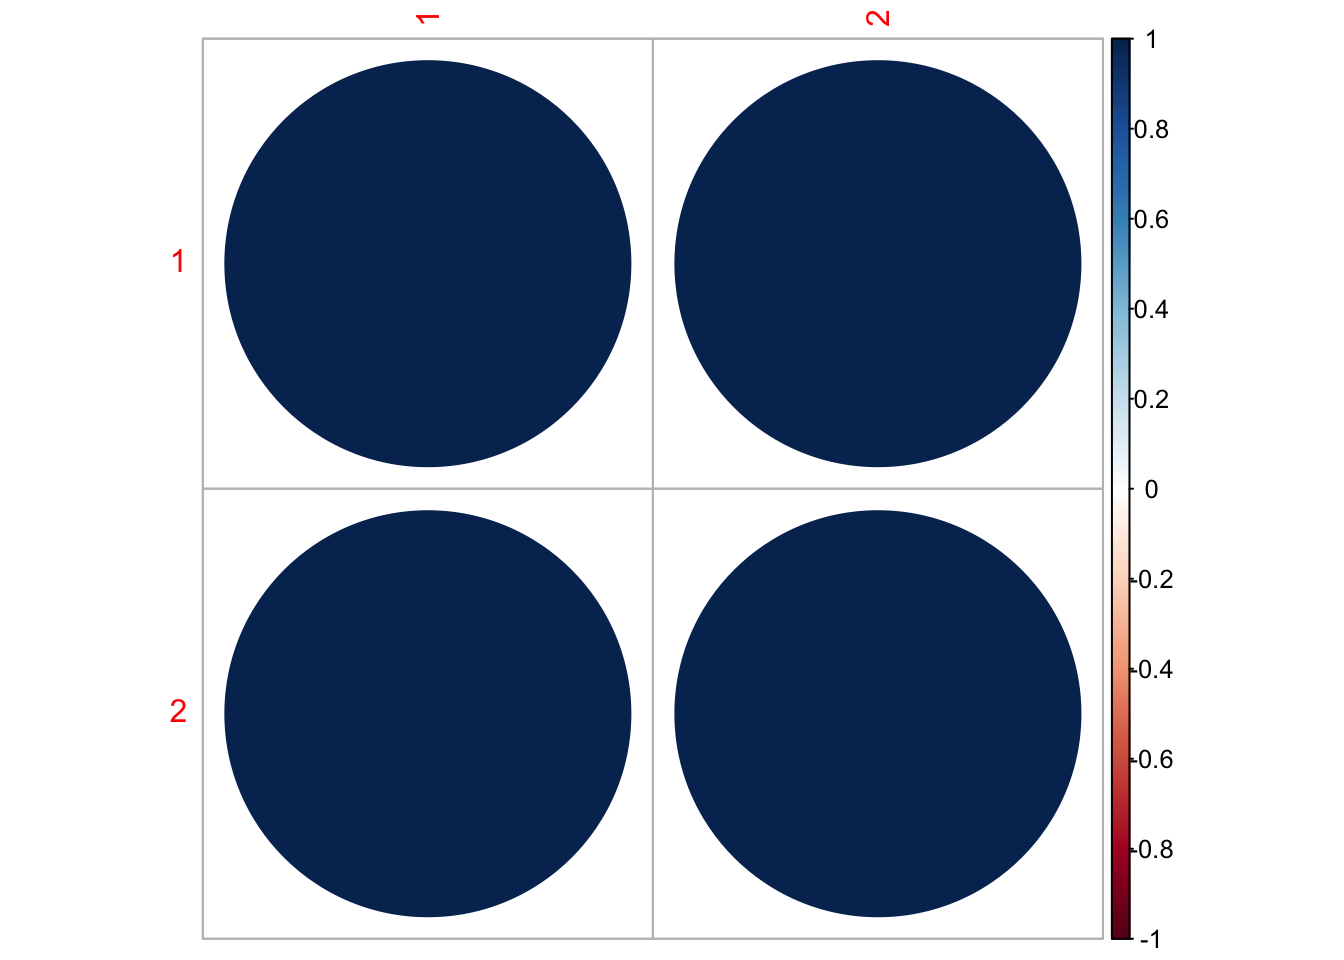
\includegraphics{Lab-1-Emma-ZR-MHS-draft_files/figure-latex/unnamed-chunk-54-1.pdf}

10 year forecast for Russia:

\begin{Shaded}
\begin{Highlighting}[]
\NormalTok{chum.russ}\OtherTok{\textless{}{-}}\FunctionTok{subset}\NormalTok{(ChumByRegion, region}\SpecialCharTok{==}\StringTok{\textquotesingle{}m\_i\textquotesingle{}}\NormalTok{)}
\NormalTok{chum.ts}\OtherTok{\textless{}{-}}\FunctionTok{ts}\NormalTok{(chum.russ}\SpecialCharTok{$}\NormalTok{lnreturns, }\AttributeTok{start=}\NormalTok{chum.russ}\SpecialCharTok{$}\NormalTok{year[}\DecValTok{1}\NormalTok{])}
\CommentTok{\#test datasets for plotting}
\NormalTok{test.russ10}\OtherTok{\textless{}{-}}\FunctionTok{window}\NormalTok{(chum.ts, }\AttributeTok{start=}\DecValTok{2006}\NormalTok{, }\AttributeTok{end=}\DecValTok{2015}\NormalTok{)}
\FunctionTok{forecast}\NormalTok{(RegionModsChum[[}\DecValTok{11}\NormalTok{]]}\SpecialCharTok{$}\NormalTok{Fit, }\AttributeTok{h =} \DecValTok{10}\NormalTok{) }\SpecialCharTok{\%\textgreater{}\%} \FunctionTok{autoplot}\NormalTok{() }\SpecialCharTok{+} \FunctionTok{geom\_point}\NormalTok{(}\FunctionTok{aes}\NormalTok{(}\AttributeTok{x=}\NormalTok{x, }\AttributeTok{y=}\NormalTok{y), }\AttributeTok{data=}\FunctionTok{fortify}\NormalTok{(test.russ10))}
\end{Highlighting}
\end{Shaded}

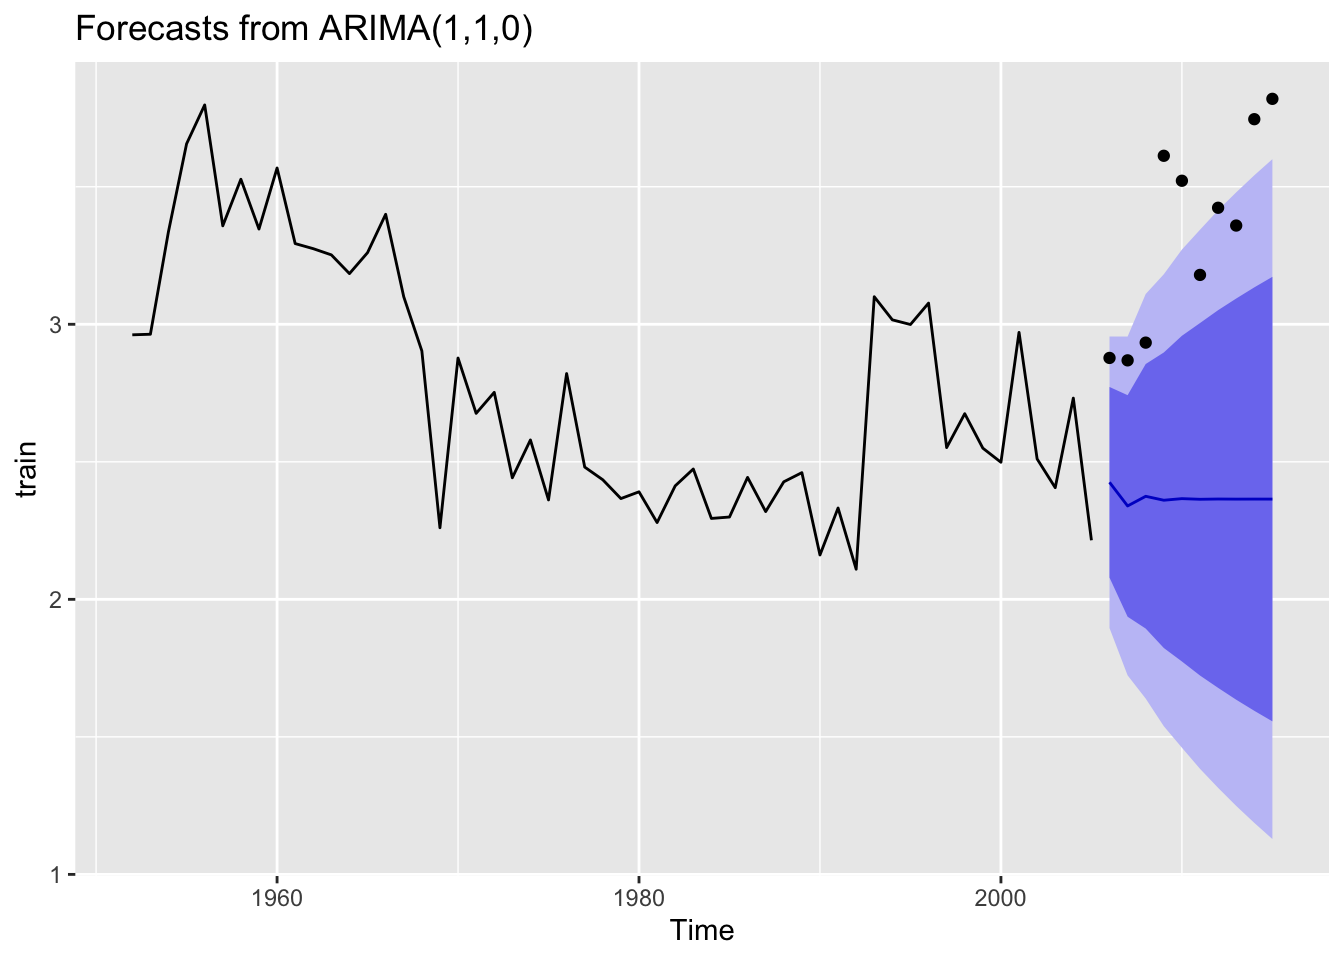
\includegraphics{Lab-1-Emma-ZR-MHS-draft_files/figure-latex/unnamed-chunk-55-1.pdf}

It looks like returns really increase at the end of the time series in
this region, which is likely why ARIMA models don't forecast this well.

Looking at stationarity:

\begin{Shaded}
\begin{Highlighting}[]
\NormalTok{Ndiff}\OtherTok{\textless{}{-}}\FunctionTok{sapply}\NormalTok{(RegionBestModChum, }\ControlFlowTok{function}\NormalTok{(x)\{}
\NormalTok{  a}\OtherTok{\textless{}{-}}\FunctionTok{strsplit}\NormalTok{(}\FunctionTok{strsplit}\NormalTok{(}\FunctionTok{strsplit}\NormalTok{(x, }\StringTok{"[(]"}\NormalTok{)[[}\DecValTok{1}\NormalTok{]][}\DecValTok{2}\NormalTok{], }\StringTok{"[)]"}\NormalTok{)[[}\DecValTok{1}\NormalTok{]][}\DecValTok{1}\NormalTok{],}\StringTok{"[,]"}\NormalTok{)}
  \FunctionTok{return}\NormalTok{(a[[}\DecValTok{1}\NormalTok{]][}\DecValTok{2}\NormalTok{])\}}
\NormalTok{)}

\FunctionTok{tibble}\NormalTok{(}\AttributeTok{Ndiff =}\NormalTok{ Ndiff, }\AttributeTok{region =}\NormalTok{ Allcombs}\SpecialCharTok{$}\NormalTok{regions, }\AttributeTok{level =}\NormalTok{ Allcombs}\SpecialCharTok{$}\NormalTok{forecastlevels) }\SpecialCharTok{\%\textgreater{}\%}
  \FunctionTok{ggplot}\NormalTok{() }\SpecialCharTok{+} \FunctionTok{geom\_bar}\NormalTok{(}\FunctionTok{aes}\NormalTok{(}\AttributeTok{x =}\NormalTok{ region, }\AttributeTok{y =}\NormalTok{ Ndiff, }\AttributeTok{fill =} \FunctionTok{as.factor}\NormalTok{(level)), }\AttributeTok{stat =} \StringTok{"identity"}\NormalTok{, }\AttributeTok{position =} \StringTok{"dodge"}\NormalTok{) }\SpecialCharTok{+}
  \FunctionTok{scale\_x\_discrete}\NormalTok{(}\AttributeTok{labels =} \FunctionTok{as\_labeller}\NormalTok{(regionskey)) }\SpecialCharTok{+}
  \FunctionTok{labs}\NormalTok{(}\AttributeTok{fill =} \StringTok{"Forecast Levels"}\NormalTok{, }\AttributeTok{x =} \StringTok{"Region"}\NormalTok{, }\AttributeTok{y =} \StringTok{"Number of Differences"}\NormalTok{) }\SpecialCharTok{+} 
  \FunctionTok{ggtitle}\NormalTok{(}\StringTok{"Number of differences to achieve stationarity (Chum)"}\NormalTok{) }\SpecialCharTok{+} \FunctionTok{theme\_bw}\NormalTok{() }\SpecialCharTok{+} \FunctionTok{theme}\NormalTok{(}\AttributeTok{axis.text.x=}\FunctionTok{element\_text}\NormalTok{(}\AttributeTok{angle=}\SpecialCharTok{{-}}\DecValTok{90}\NormalTok{, }\AttributeTok{hjust =} \DecValTok{0}\NormalTok{, }\AttributeTok{vjust =} \FloatTok{0.5}\NormalTok{ ))}
\end{Highlighting}
\end{Shaded}

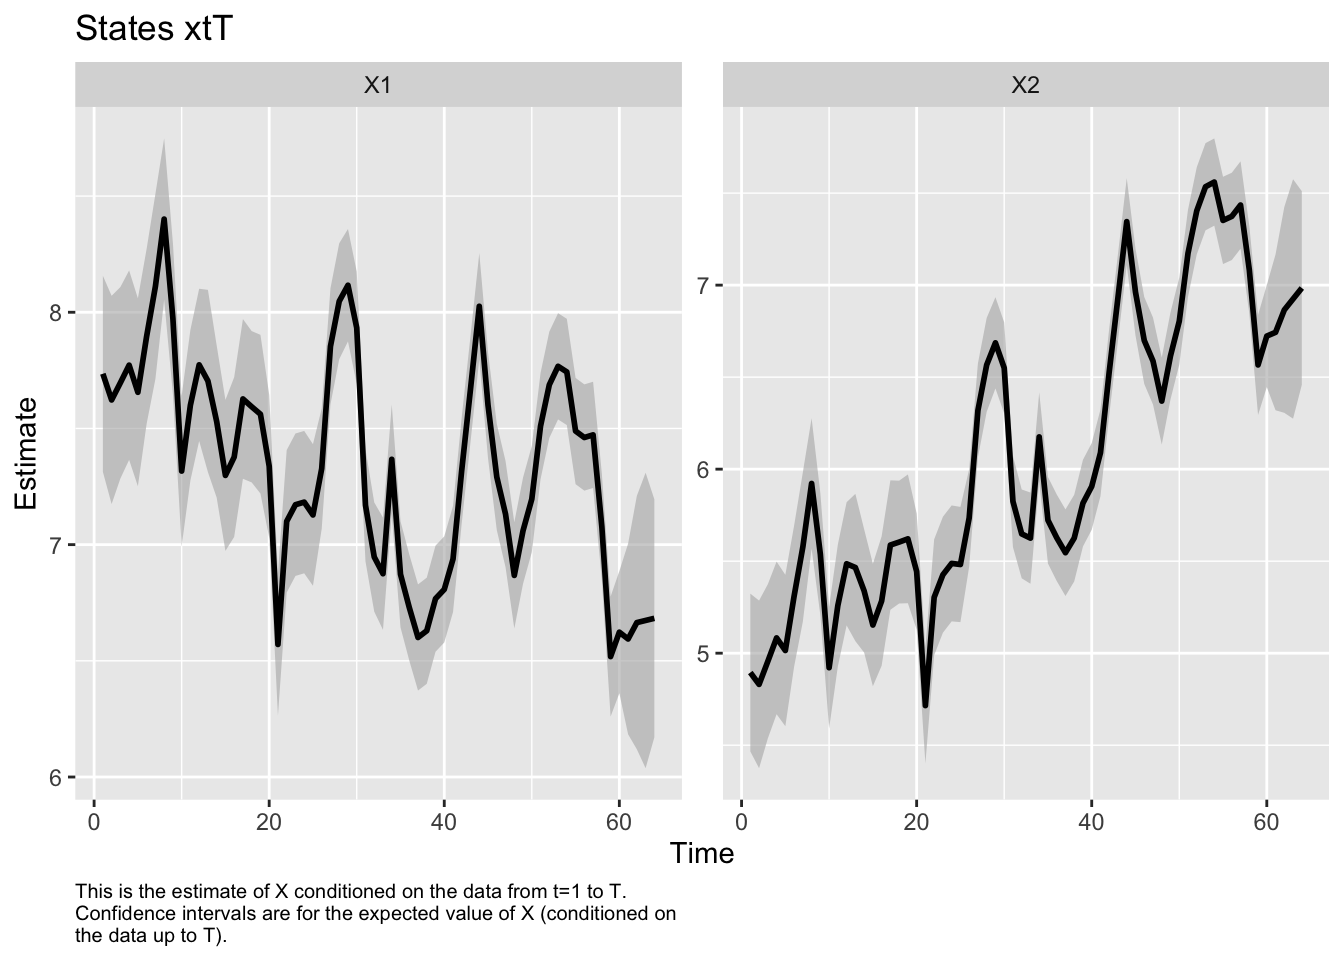
\includegraphics{Lab-1-Emma-ZR-MHS-draft_files/figure-latex/unnamed-chunk-56-1.pdf}

For Chum, time series for 5 of the regions were stationary (using tests
from auto.arima) and 7 required 1 difference to be stationary.

There was significant autocorrelation (based on Ljung-Box test) in 4 of
the regional models for Chum:

\begin{Shaded}
\begin{Highlighting}[]
\NormalTok{ac\_mods\_chum}\OtherTok{\textless{}{-}}\FunctionTok{c}\NormalTok{(}\DecValTok{26}\NormalTok{, }\DecValTok{27}\NormalTok{, }\DecValTok{31}\NormalTok{, }\DecValTok{32}\NormalTok{) }\CommentTok{\#indexes of models with autocorrelated residuals}
\ControlFlowTok{for}\NormalTok{(i }\ControlFlowTok{in} \DecValTok{1}\SpecialCharTok{:}\FunctionTok{length}\NormalTok{(ac\_mods\_chum))\{}
  \FunctionTok{print}\NormalTok{(}\FunctionTok{paste}\NormalTok{(regionskey[ResultsTableChum}\SpecialCharTok{$}\NormalTok{regions[ac\_mods\_chum[i]]], ResultsTableChum}\SpecialCharTok{$}\NormalTok{forecastlevels[ac\_mods\_chum[i]]))}
  \FunctionTok{checkresiduals}\NormalTok{(RegionModsChum[[ac\_mods\_chum[i]]]}\SpecialCharTok{$}\NormalTok{Fit)}
\NormalTok{\}}
\end{Highlighting}
\end{Shaded}

\begin{verbatim}
## [1] "SE Alaska 10"
\end{verbatim}

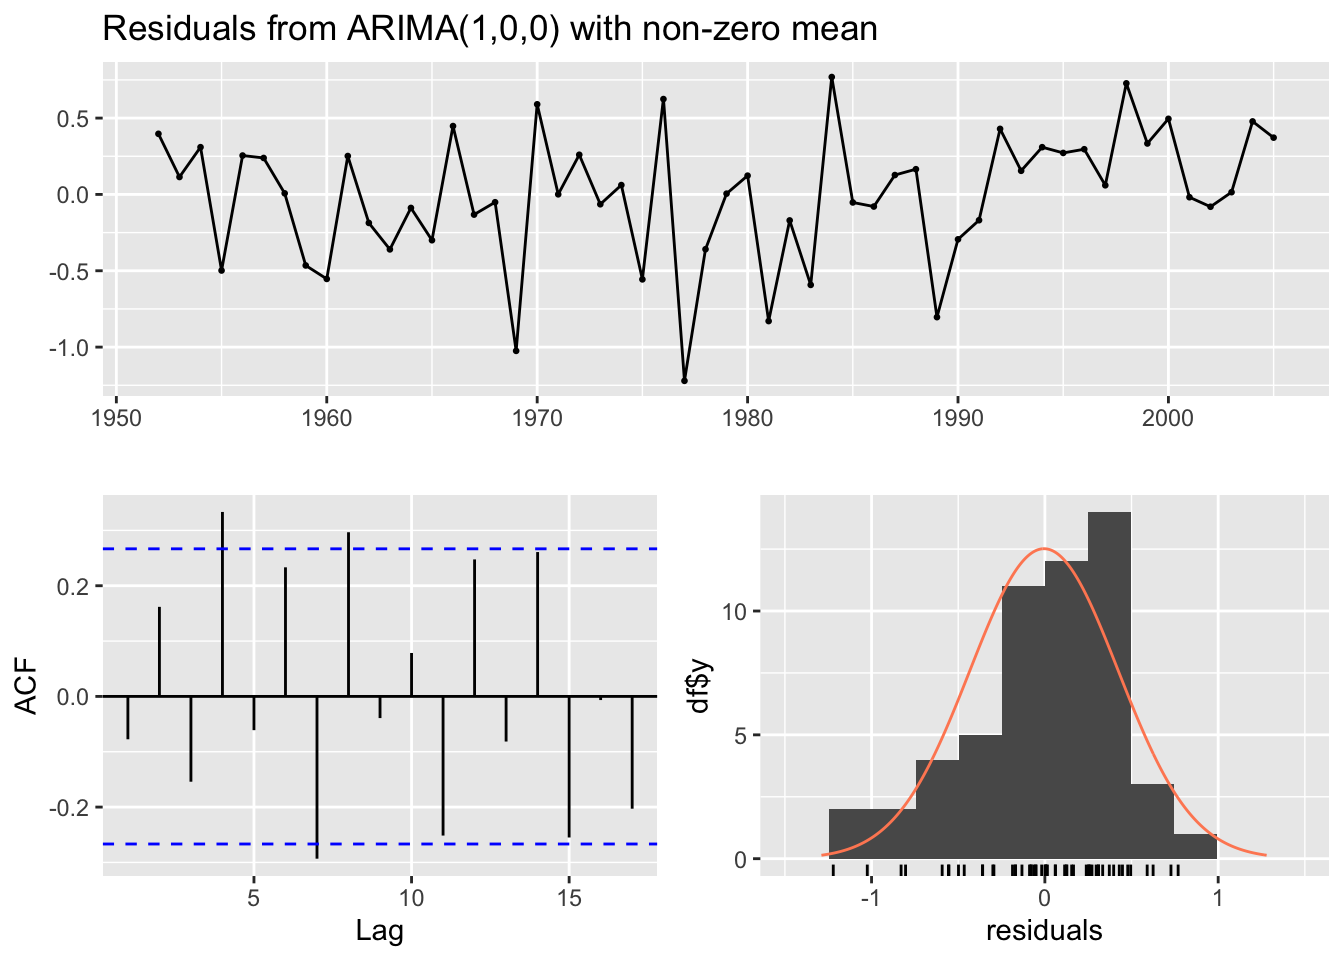
\includegraphics{Lab-1-Emma-ZR-MHS-draft_files/figure-latex/unnamed-chunk-57-1.pdf}

\begin{verbatim}
## 
##  Ljung-Box test
## 
## data:  Residuals from ARIMA(1,0,0) with non-zero mean
## Q* = 25.498, df = 9, p-value = 0.002467
## 
## Model df: 1.   Total lags used: 10
## 
## [1] "SE Alaska 20"
\end{verbatim}

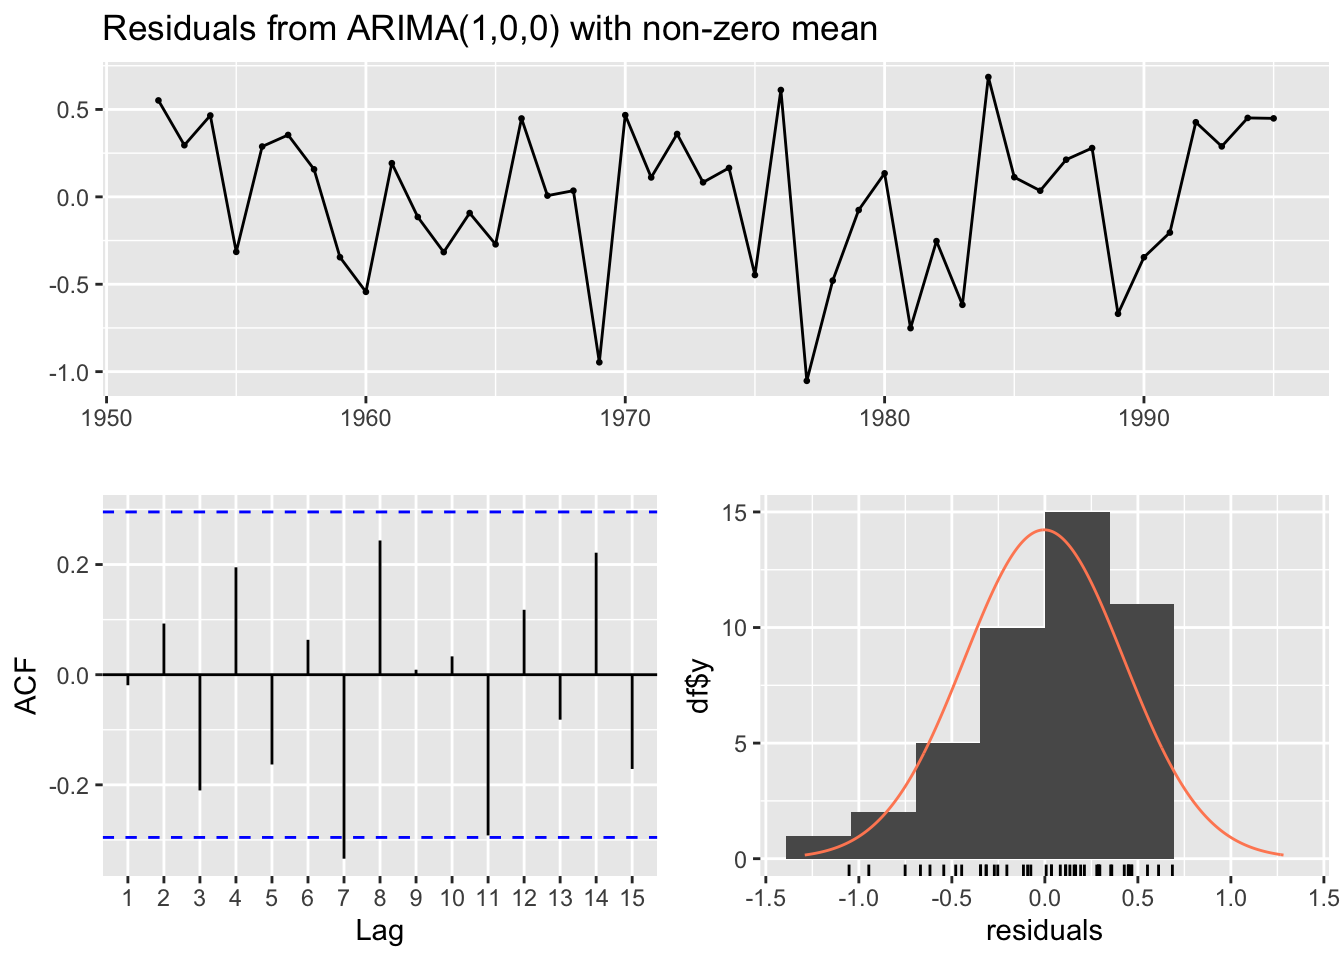
\includegraphics{Lab-1-Emma-ZR-MHS-draft_files/figure-latex/unnamed-chunk-57-2.pdf}

\begin{verbatim}
## 
##  Ljung-Box test
## 
## data:  Residuals from ARIMA(1,0,0) with non-zero mean
## Q* = 15.578, df = 8, p-value = 0.04884
## 
## Model df: 1.   Total lags used: 9
## 
## [1] "NA 5"
\end{verbatim}

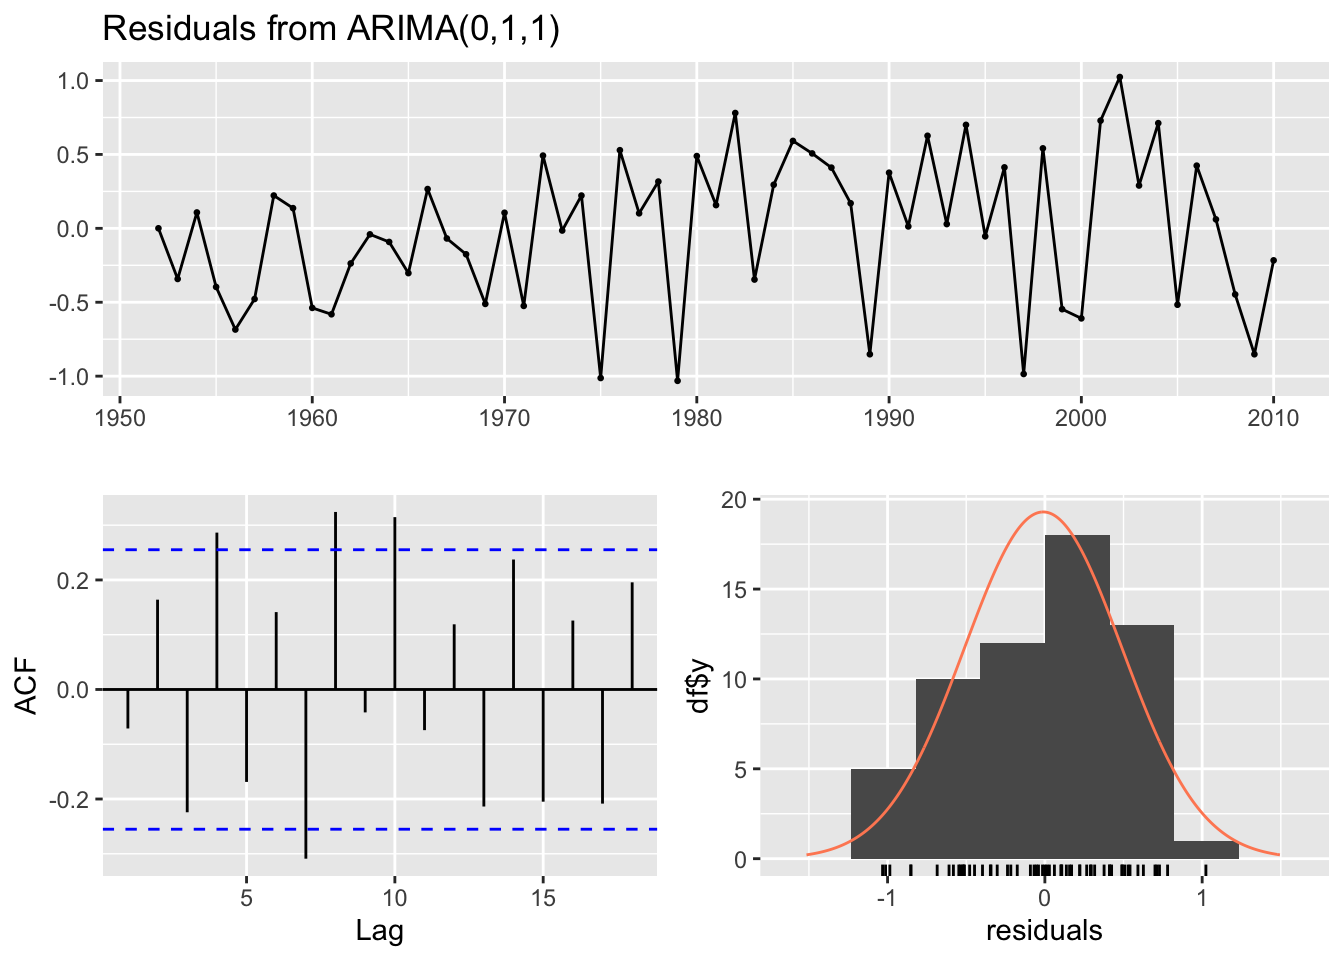
\includegraphics{Lab-1-Emma-ZR-MHS-draft_files/figure-latex/unnamed-chunk-57-3.pdf}

\begin{verbatim}
## 
##  Ljung-Box test
## 
## data:  Residuals from ARIMA(0,1,1)
## Q* = 35.287, df = 9, p-value = 5.302e-05
## 
## Model df: 1.   Total lags used: 10
## 
## [1] "NA 10"
\end{verbatim}

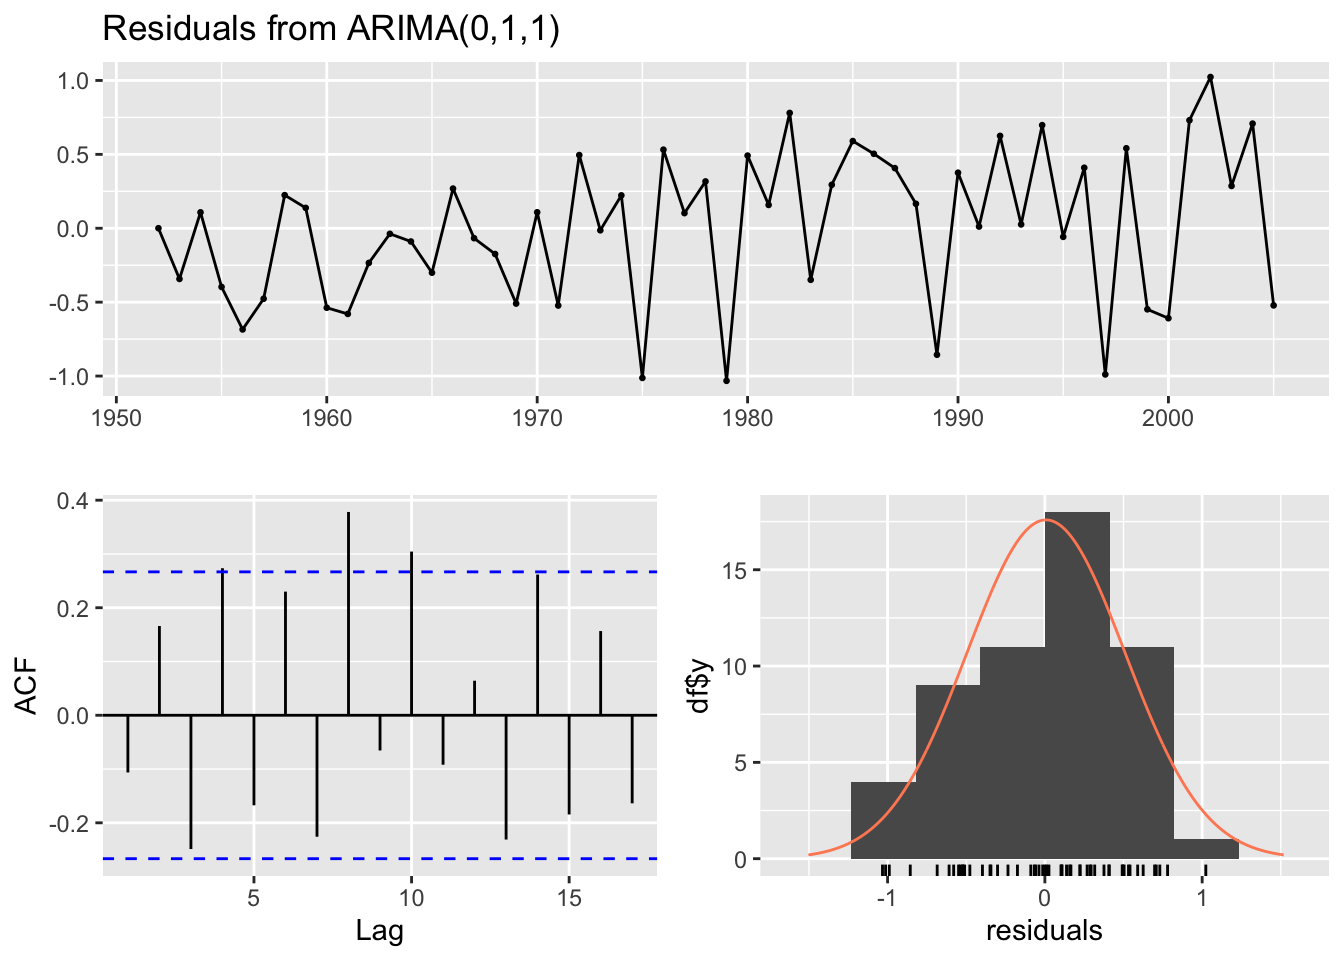
\includegraphics{Lab-1-Emma-ZR-MHS-draft_files/figure-latex/unnamed-chunk-57-4.pdf}

\begin{verbatim}
## 
##  Ljung-Box test
## 
## data:  Residuals from ARIMA(0,1,1)
## Q* = 34.843, df = 9, p-value = 6.35e-05
## 
## Model df: 1.   Total lags used: 10
\end{verbatim}

This suggests that ARIMA models may not be the best fit in this
instance.

\hypertarget{pink}{%
\subsection{Pink:}\label{pink}}

Plot MASE for three different forecast periods - 5, 10, and 20 years -
across all regions. MASE \textless{} 1 is a ``good'' value.

\begin{Shaded}
\begin{Highlighting}[]
\CommentTok{\#All Years}
\FunctionTok{ggplot}\NormalTok{(ResultsTable) }\SpecialCharTok{+} 
  \FunctionTok{geom\_bar}\NormalTok{(}\FunctionTok{aes}\NormalTok{(}\AttributeTok{x =}\NormalTok{ regions, }\AttributeTok{y =}\NormalTok{ MASE, }\AttributeTok{fill =} \FunctionTok{as.factor}\NormalTok{(forecastlevels)), }\AttributeTok{stat =} \StringTok{"identity"}\NormalTok{, }\AttributeTok{position =} \StringTok{"dodge"}\NormalTok{) }\SpecialCharTok{+} 
  \FunctionTok{geom\_hline}\NormalTok{(}\FunctionTok{aes}\NormalTok{(}\AttributeTok{yintercept =} \DecValTok{1}\NormalTok{), }\AttributeTok{linetype =} \StringTok{"dashed"}\NormalTok{) }\SpecialCharTok{+} 
  \FunctionTok{scale\_x\_discrete}\NormalTok{(}\AttributeTok{labels =} \FunctionTok{as\_labeller}\NormalTok{(regionskey)) }\SpecialCharTok{+}
  \FunctionTok{labs}\NormalTok{(}\AttributeTok{fill =} \StringTok{"Forecast Levels"}\NormalTok{, }\AttributeTok{x =} \StringTok{"Region"}\NormalTok{) }\SpecialCharTok{+} 
  \FunctionTok{ggtitle}\NormalTok{(}\StringTok{"Pinks all Years"}\NormalTok{) }\SpecialCharTok{+} \FunctionTok{theme\_bw}\NormalTok{() }\SpecialCharTok{+} \FunctionTok{theme}\NormalTok{(}\AttributeTok{axis.text.x=}\FunctionTok{element\_text}\NormalTok{(}\AttributeTok{angle=}\SpecialCharTok{{-}}\DecValTok{90}\NormalTok{, }\AttributeTok{hjust =} \DecValTok{0}\NormalTok{, }\AttributeTok{vjust =} \FloatTok{0.5}\NormalTok{ ))}
\end{Highlighting}
\end{Shaded}

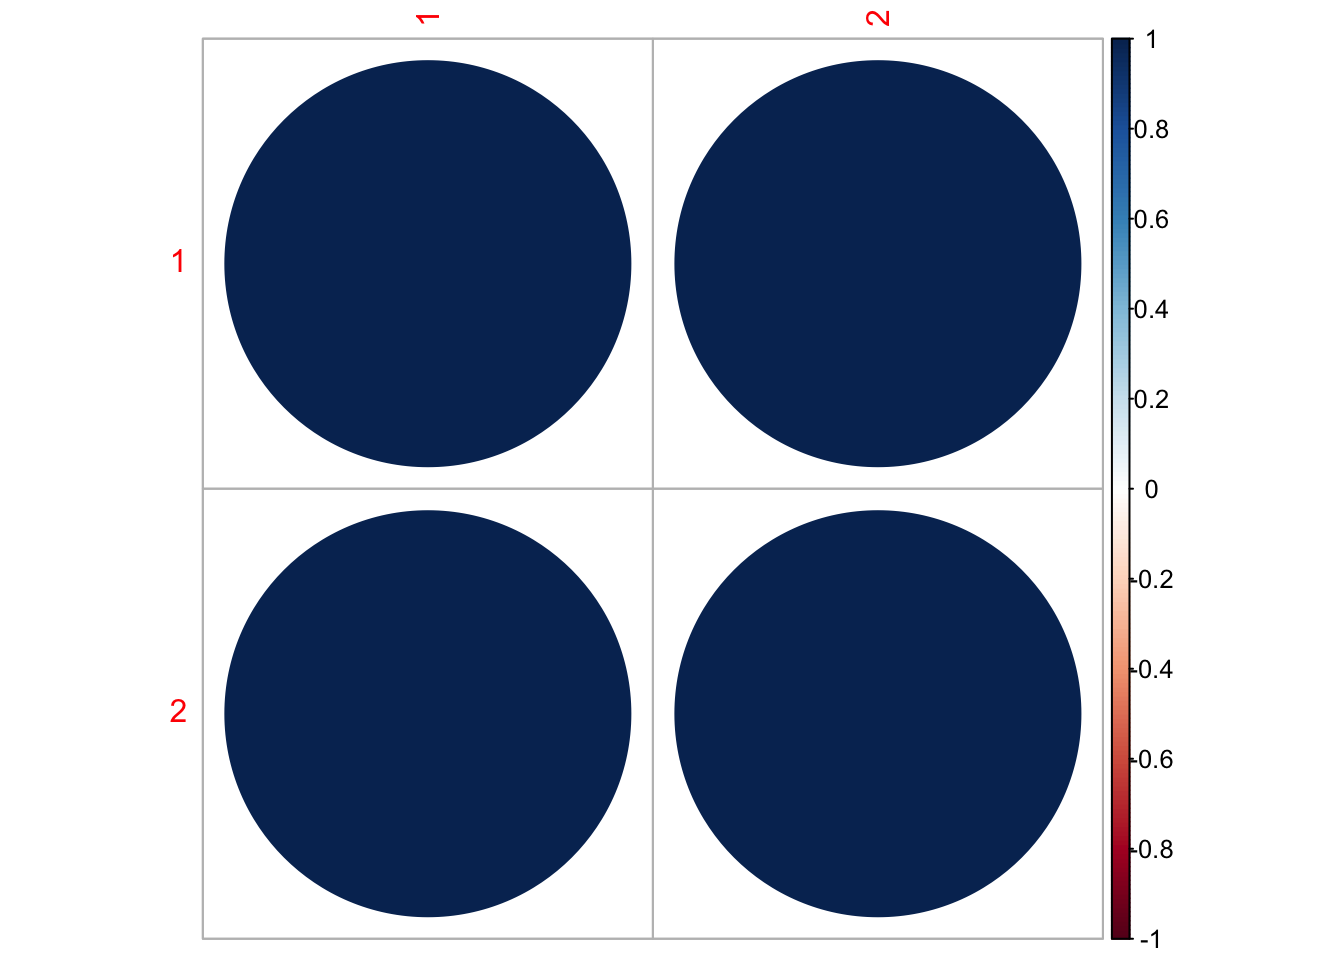
\includegraphics{Lab-1-Emma-ZR-MHS-draft_files/figure-latex/unnamed-chunk-58-1.pdf}

\begin{Shaded}
\begin{Highlighting}[]
\CommentTok{\#Even Years }
\FunctionTok{ggplot}\NormalTok{(ResultsTable\_even) }\SpecialCharTok{+} 
  \FunctionTok{geom\_bar}\NormalTok{(}\FunctionTok{aes}\NormalTok{(}\AttributeTok{x =}\NormalTok{ regions, }\AttributeTok{y =}\NormalTok{ MASE, }\AttributeTok{fill =} \FunctionTok{as.factor}\NormalTok{(forecastlevels)), }\AttributeTok{stat =} \StringTok{"identity"}\NormalTok{, }\AttributeTok{position =} \StringTok{"dodge"}\NormalTok{) }\SpecialCharTok{+} 
  \FunctionTok{geom\_hline}\NormalTok{(}\FunctionTok{aes}\NormalTok{(}\AttributeTok{yintercept =} \DecValTok{1}\NormalTok{), }\AttributeTok{linetype =} \StringTok{"dashed"}\NormalTok{) }\SpecialCharTok{+} 
  \FunctionTok{scale\_x\_discrete}\NormalTok{(}\AttributeTok{labels =} \FunctionTok{as\_labeller}\NormalTok{(regionskey)) }\SpecialCharTok{+}
  \FunctionTok{labs}\NormalTok{(}\AttributeTok{fill =} \StringTok{"Forecast Levels"}\NormalTok{, }\AttributeTok{x =} \StringTok{"Region"}\NormalTok{) }\SpecialCharTok{+} 
  \FunctionTok{ggtitle}\NormalTok{(}\StringTok{"Pinks Even Years"}\NormalTok{) }\SpecialCharTok{+} \FunctionTok{theme\_bw}\NormalTok{() }\SpecialCharTok{+} \FunctionTok{theme}\NormalTok{(}\AttributeTok{axis.text.x=}\FunctionTok{element\_text}\NormalTok{(}\AttributeTok{angle=}\SpecialCharTok{{-}}\DecValTok{90}\NormalTok{, }\AttributeTok{hjust =} \DecValTok{0}\NormalTok{, }\AttributeTok{vjust =} \FloatTok{0.5}\NormalTok{ ))}
\end{Highlighting}
\end{Shaded}

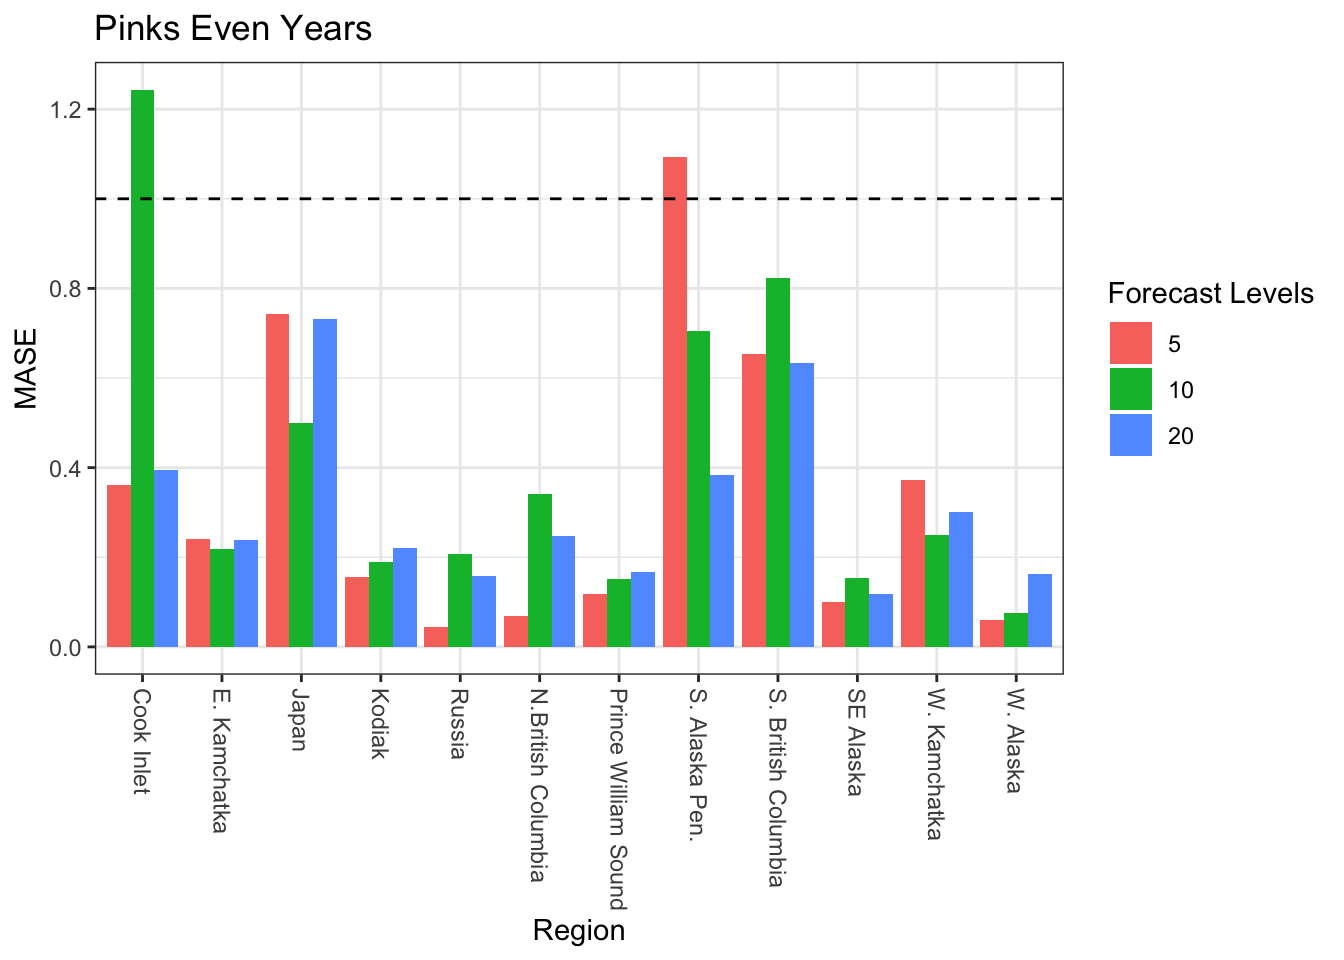
\includegraphics{Lab-1-Emma-ZR-MHS-draft_files/figure-latex/unnamed-chunk-58-2.pdf}

\begin{Shaded}
\begin{Highlighting}[]
\CommentTok{\#Odd Years }
\FunctionTok{ggplot}\NormalTok{(ResultsTable\_odd) }\SpecialCharTok{+} 
  \FunctionTok{geom\_bar}\NormalTok{(}\FunctionTok{aes}\NormalTok{(}\AttributeTok{x =}\NormalTok{ regions, }\AttributeTok{y =}\NormalTok{ MASE, }\AttributeTok{fill =} \FunctionTok{as.factor}\NormalTok{(forecastlevels)), }\AttributeTok{stat =} \StringTok{"identity"}\NormalTok{, }\AttributeTok{position =} \StringTok{"dodge"}\NormalTok{) }\SpecialCharTok{+} 
  \FunctionTok{geom\_hline}\NormalTok{(}\FunctionTok{aes}\NormalTok{(}\AttributeTok{yintercept =} \DecValTok{1}\NormalTok{), }\AttributeTok{linetype =} \StringTok{"dashed"}\NormalTok{) }\SpecialCharTok{+} 
  \FunctionTok{scale\_x\_discrete}\NormalTok{(}\AttributeTok{labels =} \FunctionTok{as\_labeller}\NormalTok{(regionskey)) }\SpecialCharTok{+}
  \FunctionTok{labs}\NormalTok{(}\AttributeTok{fill =} \StringTok{"Forecast Levels"}\NormalTok{, }\AttributeTok{x =} \StringTok{"Region"}\NormalTok{) }\SpecialCharTok{+} 
  \FunctionTok{ggtitle}\NormalTok{(}\StringTok{"Pinks Odd Years"}\NormalTok{) }\SpecialCharTok{+} \FunctionTok{theme\_bw}\NormalTok{() }\SpecialCharTok{+} \FunctionTok{theme}\NormalTok{(}\AttributeTok{axis.text.x=}\FunctionTok{element\_text}\NormalTok{(}\AttributeTok{angle=}\SpecialCharTok{{-}}\DecValTok{90}\NormalTok{, }\AttributeTok{hjust =} \DecValTok{0}\NormalTok{, }\AttributeTok{vjust =} \FloatTok{0.5}\NormalTok{ ))}
\end{Highlighting}
\end{Shaded}

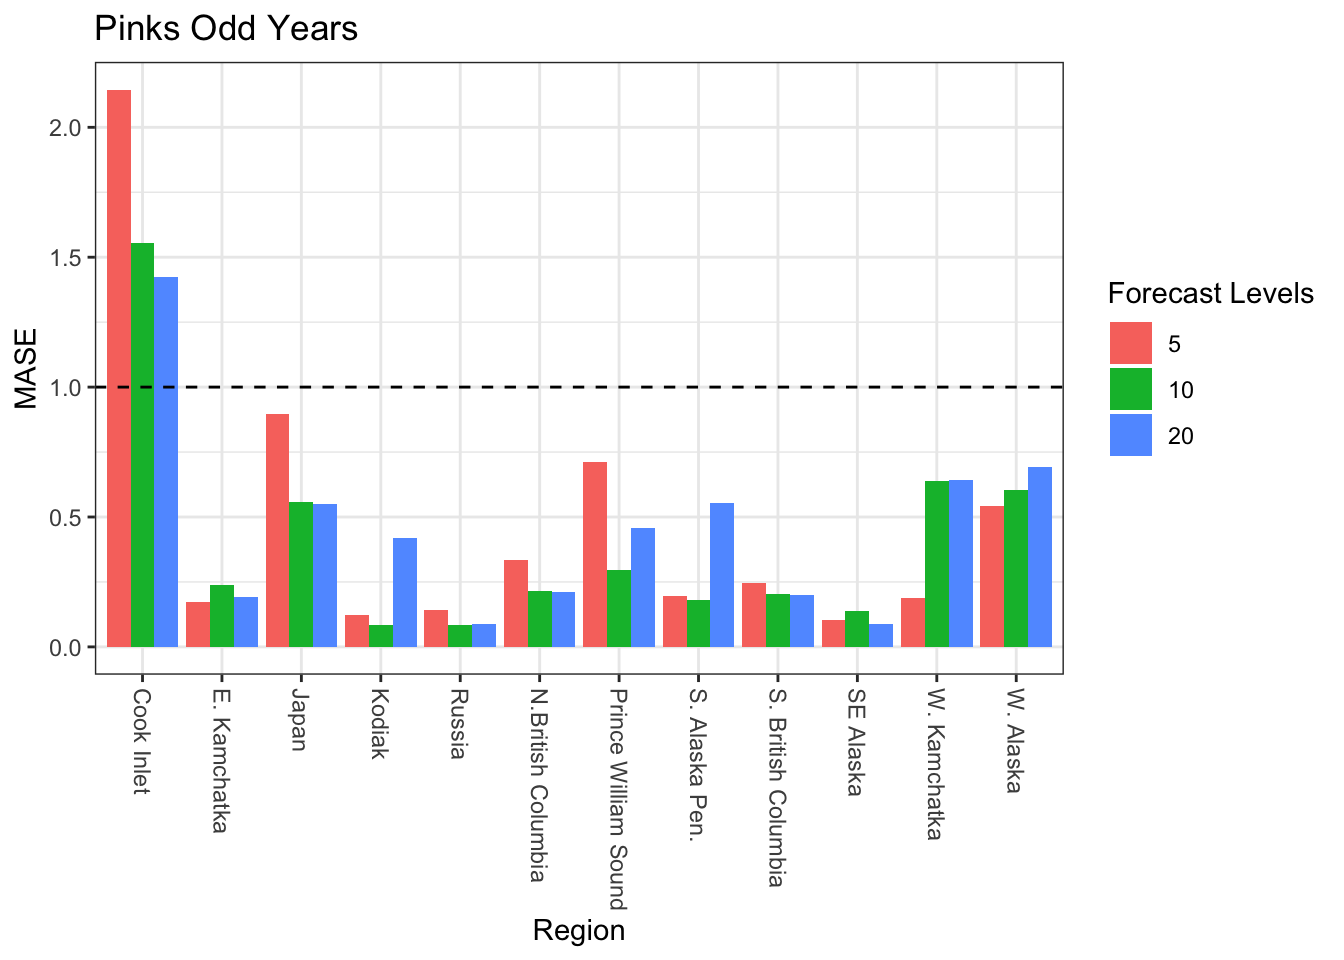
\includegraphics{Lab-1-Emma-ZR-MHS-draft_files/figure-latex/unnamed-chunk-58-3.pdf}
Despite the MASE fits seeming pretty good for the pink model runs some
of the forecasts were underwhelming. Two regions were considered for
forcasts, Cook Inlet, and SE Alaska with models that included for all
years, even years, and odd years.

The first region, Cook Inlet, performed poorly (relative to some of the
other regions) when looking at MASE values.

\begin{Shaded}
\begin{Highlighting}[]
\CommentTok{\#Cook Inlet}
\CommentTok{\#{-}{-}{-}{-}{-}{-}{-}{-}{-}{-}{-}{-}{-}{-}{-}{-}{-}{-}{-}{-}{-}{-}{-}{-}{-}{-}{-}{-}{-}{-}{-}{-}{-}{-}{-}{-}{-}{-}{-}{-}{-}{-}{-}{-}{-}{-}{-}{-}{-}{-}{-}{-}}
\CommentTok{\#All Years}
\NormalTok{pink.ci}\OtherTok{\textless{}{-}}\FunctionTok{subset}\NormalTok{(PinkByRegion, region}\SpecialCharTok{==}\StringTok{\textquotesingle{}ci\textquotesingle{}}\NormalTok{)}
\NormalTok{ci.ts}\OtherTok{\textless{}{-}}\FunctionTok{ts}\NormalTok{(pink.ci}\SpecialCharTok{$}\NormalTok{lnreturns, }\AttributeTok{start=}\NormalTok{pink.ci}\SpecialCharTok{$}\NormalTok{year[}\DecValTok{1}\NormalTok{], }\AttributeTok{frequency =} \DecValTok{1}\NormalTok{)}

\CommentTok{\#create training and test datasets for the 5 year forecast }
\NormalTok{train.ci5}\OtherTok{\textless{}{-}}\FunctionTok{window}\NormalTok{(ci.ts, }\AttributeTok{start=}\DecValTok{1952}\NormalTok{, }\AttributeTok{end=}\DecValTok{2010}\NormalTok{)}
\NormalTok{test.ci5}\OtherTok{\textless{}{-}}\FunctionTok{window}\NormalTok{(ci.ts, }\AttributeTok{start=}\DecValTok{2011}\NormalTok{, }\AttributeTok{end=}\DecValTok{2015}\NormalTok{)}
\NormalTok{ci.final5}\OtherTok{\textless{}{-}}\NormalTok{forecast}\SpecialCharTok{::}\FunctionTok{auto.arima}\NormalTok{(train.ci5, }\AttributeTok{approximation =}\NormalTok{ F, }\AttributeTok{stepwise =}\NormalTok{ F)}

\CommentTok{\#create training and test datasets for the 10 year forecast }
\NormalTok{train.ci10}\OtherTok{\textless{}{-}}\FunctionTok{window}\NormalTok{(ci.ts, }\AttributeTok{start=}\DecValTok{1952}\NormalTok{, }\AttributeTok{end=}\DecValTok{2005}\NormalTok{)}
\NormalTok{test.ci10}\OtherTok{\textless{}{-}}\FunctionTok{window}\NormalTok{(ci.ts, }\AttributeTok{start=}\DecValTok{2006}\NormalTok{, }\AttributeTok{end=}\DecValTok{2015}\NormalTok{)}
\NormalTok{ci.final10}\OtherTok{\textless{}{-}}\NormalTok{forecast}\SpecialCharTok{::}\FunctionTok{auto.arima}\NormalTok{(train.ci10, }\AttributeTok{approximation =}\NormalTok{ F, }\AttributeTok{stepwise =}\NormalTok{ F)}

\CommentTok{\#create training and test datasets for the 20 year forecast }
\NormalTok{train.ci20}\OtherTok{\textless{}{-}}\FunctionTok{window}\NormalTok{(ci.ts, }\AttributeTok{start=}\DecValTok{1952}\NormalTok{, }\AttributeTok{end=}\DecValTok{1995}\NormalTok{)}
\NormalTok{test.ci20}\OtherTok{\textless{}{-}}\FunctionTok{window}\NormalTok{(ci.ts, }\AttributeTok{start=}\DecValTok{1996}\NormalTok{, }\AttributeTok{end=}\DecValTok{2015}\NormalTok{)}
\NormalTok{ci.final20}\OtherTok{\textless{}{-}}\NormalTok{forecast}\SpecialCharTok{::}\FunctionTok{auto.arima}\NormalTok{(train.ci20, }\AttributeTok{approximation =}\NormalTok{ F, }\AttributeTok{stepwise =}\NormalTok{ F)}

\CommentTok{\#{-}{-}{-}{-}{-}{-}{-}{-}{-}{-}{-}{-}{-}{-}{-}{-}{-}{-}{-}{-}{-}{-}{-}{-}{-}{-}{-}{-}{-}{-}}
\CommentTok{\#Even Years}
\NormalTok{pink.ci\_even}\OtherTok{\textless{}{-}}\FunctionTok{subset}\NormalTok{(PinkByRegion\_even, region}\SpecialCharTok{==}\StringTok{\textquotesingle{}ci\textquotesingle{}}\NormalTok{)}
\NormalTok{ci.ts\_even}\OtherTok{\textless{}{-}}\FunctionTok{ts}\NormalTok{(pink.ci\_even}\SpecialCharTok{$}\NormalTok{lnreturns, }\AttributeTok{start=}\NormalTok{pink.ci\_even}\SpecialCharTok{$}\NormalTok{year[}\DecValTok{1}\NormalTok{], }\AttributeTok{frequency =} \FloatTok{0.5}\NormalTok{)}

\CommentTok{\#create training and test datasets for the 5 year forecast }
\NormalTok{train.ci\_even5}\OtherTok{\textless{}{-}}\FunctionTok{window}\NormalTok{(ci.ts\_even, }\AttributeTok{start=}\DecValTok{1952}\NormalTok{, }\AttributeTok{end=}\DecValTok{2010}\NormalTok{)}
\NormalTok{test.ci\_even5}\OtherTok{\textless{}{-}}\FunctionTok{window}\NormalTok{(ci.ts\_even, }\AttributeTok{start=}\DecValTok{2011}\NormalTok{, }\AttributeTok{end=}\DecValTok{2014}\NormalTok{)}
\NormalTok{ci\_even.final5}\OtherTok{\textless{}{-}}\NormalTok{forecast}\SpecialCharTok{::}\FunctionTok{auto.arima}\NormalTok{(train.ci\_even5, }\AttributeTok{approximation =}\NormalTok{ F, }\AttributeTok{stepwise =}\NormalTok{ F)}

\CommentTok{\#create training and test datasets for the 10 year forecast }
\NormalTok{train.ci\_even10}\OtherTok{\textless{}{-}}\FunctionTok{window}\NormalTok{(ci.ts\_even, }\AttributeTok{start=}\DecValTok{1952}\NormalTok{, }\AttributeTok{end=}\DecValTok{2005}\NormalTok{)}
\NormalTok{test.ci\_even10}\OtherTok{\textless{}{-}}\FunctionTok{window}\NormalTok{(ci.ts\_even, }\AttributeTok{start=}\DecValTok{2006}\NormalTok{, }\AttributeTok{end=}\DecValTok{2014}\NormalTok{)}
\NormalTok{ci\_even.final10}\OtherTok{\textless{}{-}}\NormalTok{forecast}\SpecialCharTok{::}\FunctionTok{auto.arima}\NormalTok{(train.ci\_even10, }\AttributeTok{approximation =}\NormalTok{ F, }\AttributeTok{stepwise =}\NormalTok{ F)}

\CommentTok{\#create training and test datasets for the 20 year forecast }
\NormalTok{train.ci\_even20}\OtherTok{\textless{}{-}}\FunctionTok{window}\NormalTok{(ci.ts\_even, }\AttributeTok{start=}\DecValTok{1952}\NormalTok{, }\AttributeTok{end=}\DecValTok{1995}\NormalTok{)}
\NormalTok{test.ci\_even20}\OtherTok{\textless{}{-}}\FunctionTok{window}\NormalTok{(ci.ts\_even, }\AttributeTok{start=}\DecValTok{1996}\NormalTok{, }\AttributeTok{end=}\DecValTok{2014}\NormalTok{)}
\NormalTok{ci\_even.final20}\OtherTok{\textless{}{-}}\NormalTok{forecast}\SpecialCharTok{::}\FunctionTok{auto.arima}\NormalTok{(train.ci\_even20, }\AttributeTok{approximation =}\NormalTok{ F, }\AttributeTok{stepwise =}\NormalTok{ F)}

\CommentTok{\#{-}{-}{-}{-}{-}{-}{-}{-}{-}{-}{-}{-}{-}{-}{-}{-}{-}{-}{-}{-}{-}{-}{-}{-}{-}{-}{-}{-}{-}{-}}
\CommentTok{\#Odd Years}
\NormalTok{pink.ci\_odd}\OtherTok{\textless{}{-}}\FunctionTok{subset}\NormalTok{(PinkByRegion\_odd, region}\SpecialCharTok{==}\StringTok{\textquotesingle{}ci\textquotesingle{}}\NormalTok{)}
\NormalTok{ci.ts\_odd}\OtherTok{\textless{}{-}}\FunctionTok{ts}\NormalTok{(pink.ci\_odd}\SpecialCharTok{$}\NormalTok{lnreturns, }\AttributeTok{start=}\NormalTok{pink.ci\_odd}\SpecialCharTok{$}\NormalTok{year[}\DecValTok{1}\NormalTok{], }\AttributeTok{frequency =} \FloatTok{0.5}\NormalTok{)}

\CommentTok{\#create training and test datasets for the 5 year forecast }
\NormalTok{train.ci\_odd5}\OtherTok{\textless{}{-}}\FunctionTok{window}\NormalTok{(ci.ts\_odd, }\AttributeTok{start=}\DecValTok{1953}\NormalTok{, }\AttributeTok{end=}\DecValTok{2009}\NormalTok{)}
\NormalTok{test.ci\_odd5}\OtherTok{\textless{}{-}}\FunctionTok{window}\NormalTok{(ci.ts\_odd, }\AttributeTok{start=}\DecValTok{2011}\NormalTok{, }\AttributeTok{end=}\DecValTok{2015}\NormalTok{)}
\NormalTok{ci\_odd.final5}\OtherTok{\textless{}{-}}\NormalTok{forecast}\SpecialCharTok{::}\FunctionTok{auto.arima}\NormalTok{(train.ci\_odd5, }\AttributeTok{approximation =}\NormalTok{ F, }\AttributeTok{stepwise =}\NormalTok{ F)}

\CommentTok{\#create training and test datasets for the 10 year forecast }
\NormalTok{train.ci\_odd10}\OtherTok{\textless{}{-}}\FunctionTok{window}\NormalTok{(ci.ts\_odd, }\AttributeTok{start=}\DecValTok{1953}\NormalTok{, }\AttributeTok{end=}\DecValTok{2005}\NormalTok{)}
\NormalTok{test.ci\_odd10}\OtherTok{\textless{}{-}}\FunctionTok{window}\NormalTok{(ci.ts\_odd, }\AttributeTok{start=}\DecValTok{2007}\NormalTok{, }\AttributeTok{end=}\DecValTok{2015}\NormalTok{)}
\NormalTok{ci\_odd.final10}\OtherTok{\textless{}{-}}\NormalTok{forecast}\SpecialCharTok{::}\FunctionTok{auto.arima}\NormalTok{(train.ci\_odd10, }\AttributeTok{approximation =}\NormalTok{ F, }\AttributeTok{stepwise =}\NormalTok{ F)}

\CommentTok{\#create training and test datasets for the 20 year forecast }
\NormalTok{train.ci\_odd20}\OtherTok{\textless{}{-}}\FunctionTok{window}\NormalTok{(ci.ts\_odd, }\AttributeTok{start=}\DecValTok{1953}\NormalTok{, }\AttributeTok{end=}\DecValTok{1995}\NormalTok{)}
\NormalTok{test.ci\_odd20}\OtherTok{\textless{}{-}}\FunctionTok{window}\NormalTok{(ci.ts\_odd, }\AttributeTok{start=}\DecValTok{1997}\NormalTok{, }\AttributeTok{end=}\DecValTok{2015}\NormalTok{)}
\NormalTok{ci\_odd.final20}\OtherTok{\textless{}{-}}\NormalTok{forecast}\SpecialCharTok{::}\FunctionTok{auto.arima}\NormalTok{(train.ci\_odd20, }\AttributeTok{approximation =}\NormalTok{ F, }\AttributeTok{stepwise =}\NormalTok{ F)}
\end{Highlighting}
\end{Shaded}

Let's look at forcast plots for the best performing models that consider
all data, even years, and odd years.

\begin{Shaded}
\begin{Highlighting}[]
\CommentTok{\#Plots}
\NormalTok{plot\_5 }\OtherTok{\textless{}{-}}\NormalTok{ ci.final5 }\SpecialCharTok{\%\textgreater{}\%}
  \FunctionTok{forecast}\NormalTok{(}\AttributeTok{h=}\DecValTok{5}\NormalTok{) }\SpecialCharTok{\%\textgreater{}\%}
  \FunctionTok{autoplot}\NormalTok{() }\SpecialCharTok{+} \FunctionTok{geom\_point}\NormalTok{(}\FunctionTok{aes}\NormalTok{(}\AttributeTok{x=}\NormalTok{x, }\AttributeTok{y=}\NormalTok{y), }\AttributeTok{data=}\FunctionTok{fortify}\NormalTok{(test.ci5))}

\NormalTok{plot\_10 }\OtherTok{\textless{}{-}}\NormalTok{ ci.final10 }\SpecialCharTok{\%\textgreater{}\%}
  \FunctionTok{forecast}\NormalTok{(}\AttributeTok{h=}\DecValTok{10}\NormalTok{) }\SpecialCharTok{\%\textgreater{}\%}
  \FunctionTok{autoplot}\NormalTok{() }\SpecialCharTok{+} \FunctionTok{geom\_point}\NormalTok{(}\FunctionTok{aes}\NormalTok{(}\AttributeTok{x=}\NormalTok{x, }\AttributeTok{y=}\NormalTok{y), }\AttributeTok{data=}\FunctionTok{fortify}\NormalTok{(test.ci10))}

\NormalTok{plot\_20 }\OtherTok{\textless{}{-}}\NormalTok{ ci.final20 }\SpecialCharTok{\%\textgreater{}\%}
  \FunctionTok{forecast}\NormalTok{(}\AttributeTok{h=}\DecValTok{20}\NormalTok{) }\SpecialCharTok{\%\textgreater{}\%}
  \FunctionTok{autoplot}\NormalTok{() }\SpecialCharTok{+} \FunctionTok{geom\_point}\NormalTok{(}\FunctionTok{aes}\NormalTok{(}\AttributeTok{x=}\NormalTok{x, }\AttributeTok{y=}\NormalTok{y), }\AttributeTok{data=}\FunctionTok{fortify}\NormalTok{(test.ci20))}

\NormalTok{plot\_even\_5 }\OtherTok{\textless{}{-}}\NormalTok{ ci\_even.final5 }\SpecialCharTok{\%\textgreater{}\%}
  \FunctionTok{forecast}\NormalTok{(}\AttributeTok{h=}\DecValTok{5}\NormalTok{) }\SpecialCharTok{\%\textgreater{}\%}
  \FunctionTok{autoplot}\NormalTok{() }\SpecialCharTok{+} \FunctionTok{geom\_point}\NormalTok{(}\FunctionTok{aes}\NormalTok{(}\AttributeTok{x=}\NormalTok{x, }\AttributeTok{y=}\NormalTok{y), }\AttributeTok{data=}\FunctionTok{fortify}\NormalTok{(test.ci\_even5))}

\NormalTok{plot\_even\_10 }\OtherTok{\textless{}{-}}\NormalTok{ ci\_even.final10 }\SpecialCharTok{\%\textgreater{}\%}
  \FunctionTok{forecast}\NormalTok{(}\AttributeTok{h=}\DecValTok{10}\NormalTok{) }\SpecialCharTok{\%\textgreater{}\%}
  \FunctionTok{autoplot}\NormalTok{() }\SpecialCharTok{+} \FunctionTok{geom\_point}\NormalTok{(}\FunctionTok{aes}\NormalTok{(}\AttributeTok{x=}\NormalTok{x, }\AttributeTok{y=}\NormalTok{y), }\AttributeTok{data=}\FunctionTok{fortify}\NormalTok{(test.ci\_even10))}

\NormalTok{plot\_even\_20 }\OtherTok{\textless{}{-}}\NormalTok{ ci\_even.final20 }\SpecialCharTok{\%\textgreater{}\%}
  \FunctionTok{forecast}\NormalTok{(}\AttributeTok{h=}\DecValTok{20}\NormalTok{) }\SpecialCharTok{\%\textgreater{}\%}
  \FunctionTok{autoplot}\NormalTok{() }\SpecialCharTok{+} \FunctionTok{geom\_point}\NormalTok{(}\FunctionTok{aes}\NormalTok{(}\AttributeTok{x=}\NormalTok{x, }\AttributeTok{y=}\NormalTok{y), }\AttributeTok{data=}\FunctionTok{fortify}\NormalTok{(test.ci\_even20))}

\NormalTok{plot\_odd\_5 }\OtherTok{\textless{}{-}}\NormalTok{ ci\_odd.final5 }\SpecialCharTok{\%\textgreater{}\%}
  \FunctionTok{forecast}\NormalTok{(}\AttributeTok{h=}\DecValTok{5}\NormalTok{) }\SpecialCharTok{\%\textgreater{}\%}
  \FunctionTok{autoplot}\NormalTok{() }\SpecialCharTok{+} \FunctionTok{geom\_point}\NormalTok{(}\FunctionTok{aes}\NormalTok{(}\AttributeTok{x=}\NormalTok{x, }\AttributeTok{y=}\NormalTok{y), }\AttributeTok{data=}\FunctionTok{fortify}\NormalTok{(test.ci\_odd5))}

\NormalTok{plot\_odd\_10 }\OtherTok{\textless{}{-}}\NormalTok{ ci\_odd.final10 }\SpecialCharTok{\%\textgreater{}\%}
  \FunctionTok{forecast}\NormalTok{(}\AttributeTok{h=}\DecValTok{10}\NormalTok{) }\SpecialCharTok{\%\textgreater{}\%}
  \FunctionTok{autoplot}\NormalTok{() }\SpecialCharTok{+} \FunctionTok{geom\_point}\NormalTok{(}\FunctionTok{aes}\NormalTok{(}\AttributeTok{x=}\NormalTok{x, }\AttributeTok{y=}\NormalTok{y), }\AttributeTok{data=}\FunctionTok{fortify}\NormalTok{(test.ci\_odd10))}

\NormalTok{plot\_odd\_20 }\OtherTok{\textless{}{-}}\NormalTok{ ci\_odd.final20 }\SpecialCharTok{\%\textgreater{}\%}
  \FunctionTok{forecast}\NormalTok{(}\AttributeTok{h=}\DecValTok{20}\NormalTok{) }\SpecialCharTok{\%\textgreater{}\%}
  \FunctionTok{autoplot}\NormalTok{() }\SpecialCharTok{+} \FunctionTok{geom\_point}\NormalTok{(}\FunctionTok{aes}\NormalTok{(}\AttributeTok{x=}\NormalTok{x, }\AttributeTok{y=}\NormalTok{y), }\AttributeTok{data=}\FunctionTok{fortify}\NormalTok{(test.ci\_odd20))}

\FunctionTok{plot\_grid}\NormalTok{(plot\_5, plot\_10, plot\_20, plot\_even\_5, plot\_even\_10, plot\_even\_20, plot\_odd\_5, plot\_odd\_10, plot\_odd\_20, }\AttributeTok{ncol =} \DecValTok{3}\NormalTok{, }\AttributeTok{nrow =} \DecValTok{3}\NormalTok{)}
\end{Highlighting}
\end{Shaded}

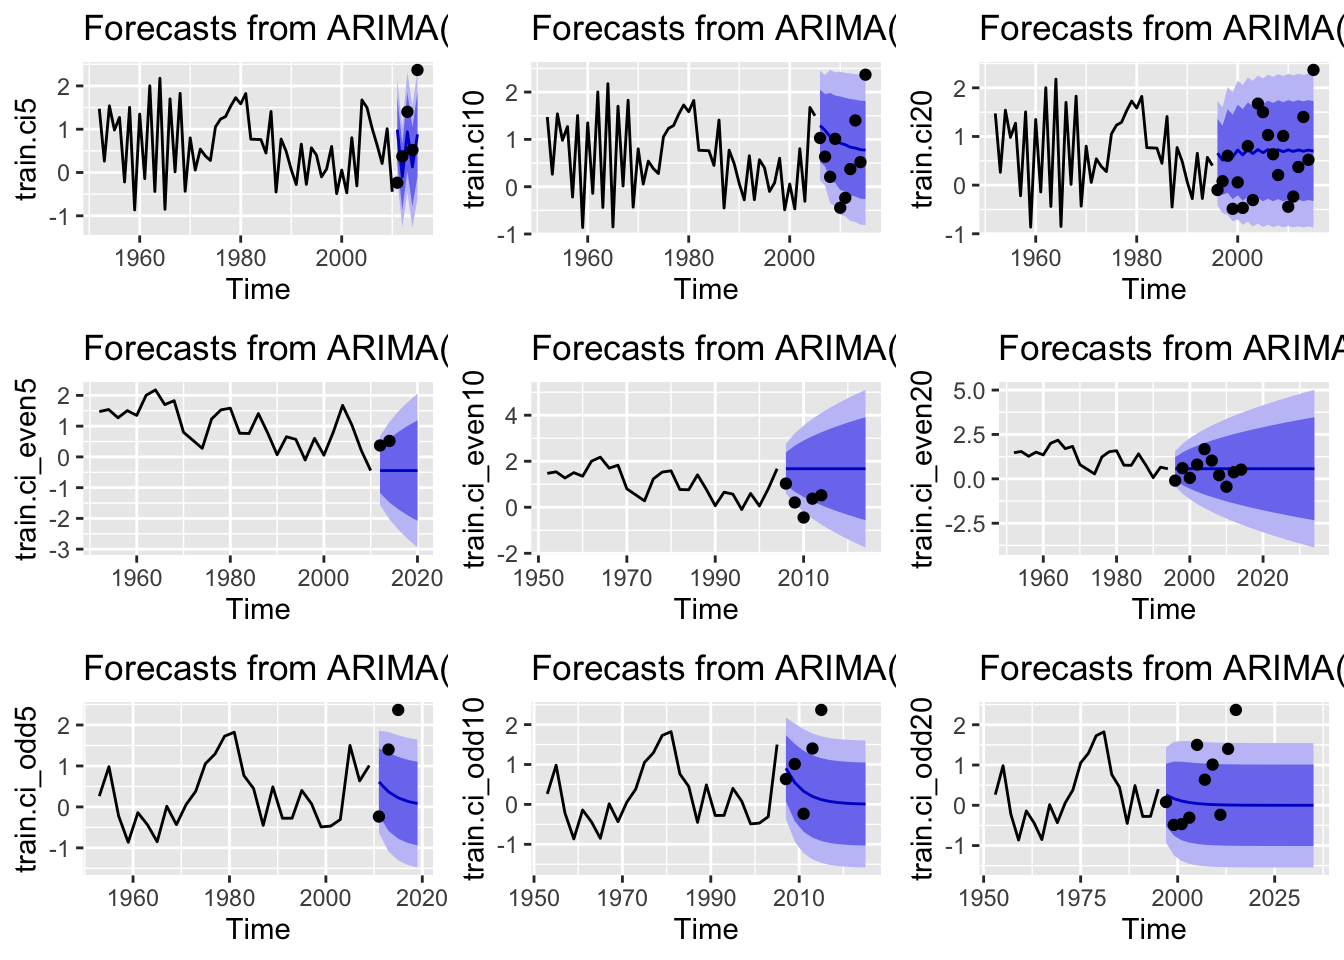
\includegraphics{Lab-1-Emma-ZR-MHS-draft_files/figure-latex/unnamed-chunk-60-1.pdf}
None of the models fit well. Let's look at one more region.

\begin{Shaded}
\begin{Highlighting}[]
\CommentTok{\#SE AK}
\CommentTok{\#{-}{-}{-}{-}{-}{-}{-}{-}{-}{-}{-}{-}{-}{-}{-}{-}{-}{-}{-}{-}{-}{-}{-}{-}{-}{-}{-}{-}{-}{-}{-}{-}{-}{-}{-}{-}{-}{-}{-}{-}{-}{-}{-}{-}{-}{-}{-}{-}{-}{-}{-}}
\CommentTok{\#All Years}
\NormalTok{pink.seak}\OtherTok{\textless{}{-}}\FunctionTok{subset}\NormalTok{(PinkByRegion, region}\SpecialCharTok{==}\StringTok{\textquotesingle{}seak\textquotesingle{}}\NormalTok{)}
\NormalTok{seak.ts}\OtherTok{\textless{}{-}}\FunctionTok{ts}\NormalTok{(pink.seak}\SpecialCharTok{$}\NormalTok{lnreturns, }\AttributeTok{start=}\NormalTok{pink.seak}\SpecialCharTok{$}\NormalTok{year[}\DecValTok{1}\NormalTok{], }\AttributeTok{frequency =} \FloatTok{0.5}\NormalTok{)}

\CommentTok{\#create training and test datasets for the 5 year forecast }
\NormalTok{train.seak5}\OtherTok{\textless{}{-}}\FunctionTok{window}\NormalTok{(seak.ts, }\AttributeTok{start=}\DecValTok{1952}\NormalTok{, }\AttributeTok{end=}\DecValTok{2010}\NormalTok{)}
\NormalTok{test.seak5}\OtherTok{\textless{}{-}}\FunctionTok{window}\NormalTok{(seak.ts, }\AttributeTok{start=}\DecValTok{2011}\NormalTok{, }\AttributeTok{end=}\DecValTok{2015}\NormalTok{)}
\NormalTok{seak.final5}\OtherTok{\textless{}{-}}\NormalTok{forecast}\SpecialCharTok{::}\FunctionTok{auto.arima}\NormalTok{(train.seak5, }\AttributeTok{approximation =}\NormalTok{ F, }\AttributeTok{stepwise =}\NormalTok{ F)}

\CommentTok{\#create training and test datasets for the 10 year forecast }
\NormalTok{train.seak10}\OtherTok{\textless{}{-}}\FunctionTok{window}\NormalTok{(seak.ts, }\AttributeTok{start=}\DecValTok{1952}\NormalTok{, }\AttributeTok{end=}\DecValTok{2005}\NormalTok{)}
\NormalTok{test.seak10}\OtherTok{\textless{}{-}}\FunctionTok{window}\NormalTok{(seak.ts, }\AttributeTok{start=}\DecValTok{2006}\NormalTok{, }\AttributeTok{end=}\DecValTok{2015}\NormalTok{)}
\NormalTok{seak.final10}\OtherTok{\textless{}{-}}\NormalTok{forecast}\SpecialCharTok{::}\FunctionTok{auto.arima}\NormalTok{(train.seak10, }\AttributeTok{approximation =}\NormalTok{ F, }\AttributeTok{stepwise =}\NormalTok{ F)}

\CommentTok{\#create training and test datasets for the 20 year forecast }
\NormalTok{train.seak20}\OtherTok{\textless{}{-}}\FunctionTok{window}\NormalTok{(seak.ts, }\AttributeTok{start=}\DecValTok{1952}\NormalTok{, }\AttributeTok{end=}\DecValTok{1995}\NormalTok{)}
\NormalTok{test.seak20}\OtherTok{\textless{}{-}}\FunctionTok{window}\NormalTok{(seak.ts, }\AttributeTok{start=}\DecValTok{1996}\NormalTok{, }\AttributeTok{end=}\DecValTok{2015}\NormalTok{)}
\NormalTok{seak.final20}\OtherTok{\textless{}{-}}\NormalTok{forecast}\SpecialCharTok{::}\FunctionTok{auto.arima}\NormalTok{(train.seak20, }\AttributeTok{approximation =}\NormalTok{ F, }\AttributeTok{stepwise =}\NormalTok{ F)}

\CommentTok{\#{-}{-}{-}{-}{-}{-}{-}{-}{-}{-}{-}{-}{-}{-}{-}{-}{-}{-}{-}{-}{-}{-}{-}{-}{-}{-}{-}{-}{-}{-}{-}{-}{-}{-}{-}{-}{-}{-}{-}{-}{-}{-}{-}{-}{-}{-}{-}{-}{-}{-}{-}{-}}
\CommentTok{\#Even Years}
\NormalTok{pink.seak\_even}\OtherTok{\textless{}{-}}\FunctionTok{subset}\NormalTok{(PinkByRegion\_even, region}\SpecialCharTok{==}\StringTok{\textquotesingle{}seak\textquotesingle{}}\NormalTok{)}
\NormalTok{seak.ts\_even}\OtherTok{\textless{}{-}}\FunctionTok{ts}\NormalTok{(pink.seak\_even}\SpecialCharTok{$}\NormalTok{lnreturns, }\AttributeTok{start=}\NormalTok{pink.seak\_even}\SpecialCharTok{$}\NormalTok{year[}\DecValTok{1}\NormalTok{], }\AttributeTok{frequency =} \FloatTok{0.5}\NormalTok{)}

\CommentTok{\#create training and test datasets for the 5 year forecast }
\NormalTok{train.seak\_even5}\OtherTok{\textless{}{-}}\FunctionTok{window}\NormalTok{(seak.ts\_even, }\AttributeTok{start=}\DecValTok{1952}\NormalTok{, }\AttributeTok{end=}\DecValTok{2010}\NormalTok{)}
\NormalTok{test.seak\_even5}\OtherTok{\textless{}{-}}\FunctionTok{window}\NormalTok{(seak.ts\_even, }\AttributeTok{start=}\DecValTok{2012}\NormalTok{, }\AttributeTok{end=}\DecValTok{2014}\NormalTok{)}
\NormalTok{seak\_even.final5}\OtherTok{\textless{}{-}}\NormalTok{forecast}\SpecialCharTok{::}\FunctionTok{auto.arima}\NormalTok{(train.seak\_even5, }\AttributeTok{approximation =}\NormalTok{ F, }\AttributeTok{stepwise =}\NormalTok{ F)}

\CommentTok{\#create training and test datasets for the 10 year forecast }
\NormalTok{train.seak\_even10}\OtherTok{\textless{}{-}}\FunctionTok{window}\NormalTok{(seak.ts\_even, }\AttributeTok{start=}\DecValTok{1952}\NormalTok{, }\AttributeTok{end=}\DecValTok{2004}\NormalTok{)}
\NormalTok{test.seak\_even10}\OtherTok{\textless{}{-}}\FunctionTok{window}\NormalTok{(seak.ts\_even, }\AttributeTok{start=}\DecValTok{2006}\NormalTok{, }\AttributeTok{end=}\DecValTok{2014}\NormalTok{)}
\NormalTok{seak\_even.final10}\OtherTok{\textless{}{-}}\NormalTok{forecast}\SpecialCharTok{::}\FunctionTok{auto.arima}\NormalTok{(train.seak\_even10, }\AttributeTok{approximation =}\NormalTok{ F, }\AttributeTok{stepwise =}\NormalTok{ F)}

\CommentTok{\#create training and test datasets for the 20 year forecast }
\NormalTok{train.seak\_even20}\OtherTok{\textless{}{-}}\FunctionTok{window}\NormalTok{(seak.ts\_even, }\AttributeTok{start=}\DecValTok{1952}\NormalTok{, }\AttributeTok{end=}\DecValTok{1994}\NormalTok{)}
\NormalTok{test.seak\_even20}\OtherTok{\textless{}{-}}\FunctionTok{window}\NormalTok{(seak.ts\_even, }\AttributeTok{start=}\DecValTok{1996}\NormalTok{, }\AttributeTok{end=}\DecValTok{2014}\NormalTok{)}
\NormalTok{seak\_even.final20}\OtherTok{\textless{}{-}}\NormalTok{forecast}\SpecialCharTok{::}\FunctionTok{auto.arima}\NormalTok{(train.seak\_even20, }\AttributeTok{approximation =}\NormalTok{ F, }\AttributeTok{stepwise =}\NormalTok{ F)}

\CommentTok{\#{-}{-}{-}{-}{-}{-}{-}{-}{-}{-}{-}{-}{-}{-}{-}{-}{-}{-}{-}{-}{-}{-}{-}{-}{-}{-}{-}{-}{-}{-}}
\CommentTok{\#Odd Years}
\NormalTok{pink.seak\_odd}\OtherTok{\textless{}{-}}\FunctionTok{subset}\NormalTok{(PinkByRegion\_odd, region}\SpecialCharTok{==}\StringTok{\textquotesingle{}seak\textquotesingle{}}\NormalTok{)}
\NormalTok{seak.ts\_odd}\OtherTok{\textless{}{-}}\FunctionTok{ts}\NormalTok{(pink.seak\_odd}\SpecialCharTok{$}\NormalTok{lnreturns, }\AttributeTok{start=}\NormalTok{pink.seak\_odd}\SpecialCharTok{$}\NormalTok{year[}\DecValTok{1}\NormalTok{], }\AttributeTok{frequency =} \FloatTok{0.5}\NormalTok{)}

\CommentTok{\#create training and test datasets for the 5 year forecast }
\NormalTok{train.seak\_odd5}\OtherTok{\textless{}{-}}\FunctionTok{window}\NormalTok{(seak.ts\_odd, }\AttributeTok{start=}\DecValTok{1953}\NormalTok{, }\AttributeTok{end=}\DecValTok{2009}\NormalTok{)}
\NormalTok{test.seak\_odd5}\OtherTok{\textless{}{-}}\FunctionTok{window}\NormalTok{(seak.ts\_odd, }\AttributeTok{start=}\DecValTok{2011}\NormalTok{, }\AttributeTok{end=}\DecValTok{2015}\NormalTok{)}
\NormalTok{seak\_odd.final5}\OtherTok{\textless{}{-}}\NormalTok{forecast}\SpecialCharTok{::}\FunctionTok{auto.arima}\NormalTok{(train.seak\_odd5, }\AttributeTok{approximation =}\NormalTok{ F, }\AttributeTok{stepwise =}\NormalTok{ F)}

\CommentTok{\#create training and test datasets for the 10 year forecast }
\NormalTok{train.seak\_odd10}\OtherTok{\textless{}{-}}\FunctionTok{window}\NormalTok{(seak.ts\_odd, }\AttributeTok{start=}\DecValTok{1953}\NormalTok{, }\AttributeTok{end=}\DecValTok{2005}\NormalTok{)}
\NormalTok{test.seak\_odd10}\OtherTok{\textless{}{-}}\FunctionTok{window}\NormalTok{(seak.ts\_odd, }\AttributeTok{start=}\DecValTok{2007}\NormalTok{, }\AttributeTok{end=}\DecValTok{2015}\NormalTok{)}
\NormalTok{seak\_odd.final10}\OtherTok{\textless{}{-}}\NormalTok{forecast}\SpecialCharTok{::}\FunctionTok{auto.arima}\NormalTok{(train.seak\_odd10, }\AttributeTok{approximation =}\NormalTok{ F, }\AttributeTok{stepwise =}\NormalTok{ F)}

\CommentTok{\#create training and test datasets for the 20 year forecast }
\NormalTok{train.seak\_odd20}\OtherTok{\textless{}{-}}\FunctionTok{window}\NormalTok{(seak.ts\_odd, }\AttributeTok{start=}\DecValTok{1953}\NormalTok{, }\AttributeTok{end=}\DecValTok{1995}\NormalTok{)}
\NormalTok{test.seak\_odd20}\OtherTok{\textless{}{-}}\FunctionTok{window}\NormalTok{(seak.ts\_odd, }\AttributeTok{start=}\DecValTok{1997}\NormalTok{, }\AttributeTok{end=}\DecValTok{2015}\NormalTok{)}
\NormalTok{seak\_odd.final20}\OtherTok{\textless{}{-}}\NormalTok{forecast}\SpecialCharTok{::}\FunctionTok{auto.arima}\NormalTok{(train.seak\_odd20, }\AttributeTok{approximation =}\NormalTok{ F, }\AttributeTok{stepwise =}\NormalTok{ F)}
\end{Highlighting}
\end{Shaded}

Let's look at forcast plots for the best performing models that consider
all data, even years, and odd years.

\begin{Shaded}
\begin{Highlighting}[]
\CommentTok{\#Plots }
\NormalTok{plot\_5 }\OtherTok{\textless{}{-}}\NormalTok{ seak.final5 }\SpecialCharTok{\%\textgreater{}\%}
  \FunctionTok{forecast}\NormalTok{(}\AttributeTok{h=}\DecValTok{5}\NormalTok{) }\SpecialCharTok{\%\textgreater{}\%}
  \FunctionTok{autoplot}\NormalTok{() }\SpecialCharTok{+} \FunctionTok{geom\_point}\NormalTok{(}\FunctionTok{aes}\NormalTok{(}\AttributeTok{x=}\NormalTok{x, }\AttributeTok{y=}\NormalTok{y), }\AttributeTok{data=}\FunctionTok{fortify}\NormalTok{(test.seak5))}

\NormalTok{plot\_10 }\OtherTok{\textless{}{-}}\NormalTok{ seak.final10 }\SpecialCharTok{\%\textgreater{}\%}
  \FunctionTok{forecast}\NormalTok{(}\AttributeTok{h=}\DecValTok{10}\NormalTok{) }\SpecialCharTok{\%\textgreater{}\%}
  \FunctionTok{autoplot}\NormalTok{() }\SpecialCharTok{+} \FunctionTok{geom\_point}\NormalTok{(}\FunctionTok{aes}\NormalTok{(}\AttributeTok{x=}\NormalTok{x, }\AttributeTok{y=}\NormalTok{y), }\AttributeTok{data=}\FunctionTok{fortify}\NormalTok{(test.seak10))}

\NormalTok{plot\_20 }\OtherTok{\textless{}{-}}\NormalTok{ seak.final20 }\SpecialCharTok{\%\textgreater{}\%}
  \FunctionTok{forecast}\NormalTok{(}\AttributeTok{h=}\DecValTok{20}\NormalTok{) }\SpecialCharTok{\%\textgreater{}\%}
  \FunctionTok{autoplot}\NormalTok{() }\SpecialCharTok{+} \FunctionTok{geom\_point}\NormalTok{(}\FunctionTok{aes}\NormalTok{(}\AttributeTok{x=}\NormalTok{x, }\AttributeTok{y=}\NormalTok{y), }\AttributeTok{data=}\FunctionTok{fortify}\NormalTok{(test.seak20))}

\NormalTok{plot\_even\_5 }\OtherTok{\textless{}{-}}\NormalTok{ seak\_even.final5 }\SpecialCharTok{\%\textgreater{}\%}
  \FunctionTok{forecast}\NormalTok{(}\AttributeTok{h=}\DecValTok{5}\NormalTok{) }\SpecialCharTok{\%\textgreater{}\%}
  \FunctionTok{autoplot}\NormalTok{() }\SpecialCharTok{+} \FunctionTok{geom\_point}\NormalTok{(}\FunctionTok{aes}\NormalTok{(}\AttributeTok{x=}\NormalTok{x, }\AttributeTok{y=}\NormalTok{y), }\AttributeTok{data=}\FunctionTok{fortify}\NormalTok{(test.seak\_even5))}

\NormalTok{plot\_even\_10 }\OtherTok{\textless{}{-}}\NormalTok{ seak\_even.final10 }\SpecialCharTok{\%\textgreater{}\%}
  \FunctionTok{forecast}\NormalTok{(}\AttributeTok{h=}\DecValTok{10}\NormalTok{) }\SpecialCharTok{\%\textgreater{}\%}
  \FunctionTok{autoplot}\NormalTok{() }\SpecialCharTok{+} \FunctionTok{geom\_point}\NormalTok{(}\FunctionTok{aes}\NormalTok{(}\AttributeTok{x=}\NormalTok{x, }\AttributeTok{y=}\NormalTok{y), }\AttributeTok{data=}\FunctionTok{fortify}\NormalTok{(test.seak\_even10))}

\NormalTok{plot\_even\_20 }\OtherTok{\textless{}{-}}\NormalTok{ seak\_even.final20 }\SpecialCharTok{\%\textgreater{}\%}
  \FunctionTok{forecast}\NormalTok{(}\AttributeTok{h=}\DecValTok{20}\NormalTok{) }\SpecialCharTok{\%\textgreater{}\%}
  \FunctionTok{autoplot}\NormalTok{() }\SpecialCharTok{+} \FunctionTok{geom\_point}\NormalTok{(}\FunctionTok{aes}\NormalTok{(}\AttributeTok{x=}\NormalTok{x, }\AttributeTok{y=}\NormalTok{y), }\AttributeTok{data=}\FunctionTok{fortify}\NormalTok{(test.seak\_even20))}

\NormalTok{plot\_odd\_5 }\OtherTok{\textless{}{-}}\NormalTok{ seak\_odd.final5 }\SpecialCharTok{\%\textgreater{}\%}
  \FunctionTok{forecast}\NormalTok{(}\AttributeTok{h=}\DecValTok{5}\NormalTok{) }\SpecialCharTok{\%\textgreater{}\%}
  \FunctionTok{autoplot}\NormalTok{() }\SpecialCharTok{+} \FunctionTok{geom\_point}\NormalTok{(}\FunctionTok{aes}\NormalTok{(}\AttributeTok{x=}\NormalTok{x, }\AttributeTok{y=}\NormalTok{y), }\AttributeTok{data=}\FunctionTok{fortify}\NormalTok{(test.seak\_odd5))}

\NormalTok{plot\_odd\_10 }\OtherTok{\textless{}{-}}\NormalTok{ seak\_odd.final10 }\SpecialCharTok{\%\textgreater{}\%}
  \FunctionTok{forecast}\NormalTok{(}\AttributeTok{h=}\DecValTok{10}\NormalTok{) }\SpecialCharTok{\%\textgreater{}\%}
  \FunctionTok{autoplot}\NormalTok{() }\SpecialCharTok{+} \FunctionTok{geom\_point}\NormalTok{(}\FunctionTok{aes}\NormalTok{(}\AttributeTok{x=}\NormalTok{x, }\AttributeTok{y=}\NormalTok{y), }\AttributeTok{data=}\FunctionTok{fortify}\NormalTok{(test.seak\_odd10))}

\NormalTok{plot\_odd\_20 }\OtherTok{\textless{}{-}}\NormalTok{ seak\_odd.final20 }\SpecialCharTok{\%\textgreater{}\%}
  \FunctionTok{forecast}\NormalTok{(}\AttributeTok{h=}\DecValTok{20}\NormalTok{) }\SpecialCharTok{\%\textgreater{}\%}
  \FunctionTok{autoplot}\NormalTok{() }\SpecialCharTok{+} \FunctionTok{geom\_point}\NormalTok{(}\FunctionTok{aes}\NormalTok{(}\AttributeTok{x=}\NormalTok{x, }\AttributeTok{y=}\NormalTok{y), }\AttributeTok{data=}\FunctionTok{fortify}\NormalTok{(test.seak\_odd20))}

\FunctionTok{plot\_grid}\NormalTok{(plot\_5, plot\_10, plot\_20, plot\_even\_5, plot\_even\_10, plot\_even\_20, plot\_odd\_5, plot\_odd\_10, plot\_odd\_20, }\AttributeTok{ncol =} \DecValTok{3}\NormalTok{, }\AttributeTok{nrow =} \DecValTok{3}\NormalTok{)}
\end{Highlighting}
\end{Shaded}

\includegraphics{Lab-1-Emma-ZR-MHS-draft_files/figure-latex/unnamed-chunk-62-1.pdf}
These models were all pretty flat and also didn't seem to capture the
trends particularly well.

Next, the number of models that had a differencing was plotted for all
years, even years, and odd years.

\begin{Shaded}
\begin{Highlighting}[]
\CommentTok{\#All Years }
\NormalTok{Ndiff}\OtherTok{\textless{}{-}}\FunctionTok{sapply}\NormalTok{(RegionBestMod, }\ControlFlowTok{function}\NormalTok{(x)\{}
\NormalTok{  a}\OtherTok{\textless{}{-}}\FunctionTok{strsplit}\NormalTok{(}\FunctionTok{strsplit}\NormalTok{(}\FunctionTok{strsplit}\NormalTok{(x, }\StringTok{"[(]"}\NormalTok{)[[}\DecValTok{1}\NormalTok{]][}\DecValTok{2}\NormalTok{], }\StringTok{"[)]"}\NormalTok{)[[}\DecValTok{1}\NormalTok{]][}\DecValTok{1}\NormalTok{],}\StringTok{"[,]"}\NormalTok{)}
  \FunctionTok{return}\NormalTok{(a[[}\DecValTok{1}\NormalTok{]][}\DecValTok{2}\NormalTok{])\}}
\NormalTok{)}

\FunctionTok{tibble}\NormalTok{(}\AttributeTok{Ndiff =}\NormalTok{ Ndiff, }\AttributeTok{region =}\NormalTok{ Allcombs}\SpecialCharTok{$}\NormalTok{regions, }\AttributeTok{level =}\NormalTok{ Allcombs}\SpecialCharTok{$}\NormalTok{forecastlevels) }\SpecialCharTok{\%\textgreater{}\%}
  \FunctionTok{ggplot}\NormalTok{() }\SpecialCharTok{+} \FunctionTok{geom\_bar}\NormalTok{(}\FunctionTok{aes}\NormalTok{(}\AttributeTok{x =}\NormalTok{ region, }\AttributeTok{y =}\NormalTok{ Ndiff, }\AttributeTok{fill =} \FunctionTok{as.factor}\NormalTok{(level)), }\AttributeTok{stat =} \StringTok{"identity"}\NormalTok{, }\AttributeTok{position =} \StringTok{"dodge"}\NormalTok{) }\SpecialCharTok{+}
  \FunctionTok{scale\_x\_discrete}\NormalTok{(}\AttributeTok{labels =} \FunctionTok{as\_labeller}\NormalTok{(regionskey)) }\SpecialCharTok{+}
  \FunctionTok{labs}\NormalTok{(}\AttributeTok{fill =} \StringTok{"Forecast Levels"}\NormalTok{, }\AttributeTok{x =} \StringTok{"Region"}\NormalTok{, }\AttributeTok{y =} \StringTok{"Number of Differences"}\NormalTok{) }\SpecialCharTok{+} 
  \FunctionTok{ggtitle}\NormalTok{(}\StringTok{"Number of differences to achieve stationarity (Pink{-}All Years)"}\NormalTok{) }\SpecialCharTok{+} \FunctionTok{theme\_bw}\NormalTok{() }\SpecialCharTok{+} \FunctionTok{theme}\NormalTok{(}\AttributeTok{axis.text.x=}\FunctionTok{element\_text}\NormalTok{(}\AttributeTok{angle=}\SpecialCharTok{{-}}\DecValTok{90}\NormalTok{, }\AttributeTok{hjust =} \DecValTok{0}\NormalTok{, }\AttributeTok{vjust =} \FloatTok{0.5}\NormalTok{ ))}
\end{Highlighting}
\end{Shaded}

\includegraphics{Lab-1-Emma-ZR-MHS-draft_files/figure-latex/unnamed-chunk-63-1.pdf}

\begin{Shaded}
\begin{Highlighting}[]
\CommentTok{\#Even Years }
\NormalTok{Ndiff\_even}\OtherTok{\textless{}{-}}\FunctionTok{sapply}\NormalTok{(RegionBestMod\_even, }\ControlFlowTok{function}\NormalTok{(x)\{}
\NormalTok{  a}\OtherTok{\textless{}{-}}\FunctionTok{strsplit}\NormalTok{(}\FunctionTok{strsplit}\NormalTok{(}\FunctionTok{strsplit}\NormalTok{(x, }\StringTok{"[(]"}\NormalTok{)[[}\DecValTok{1}\NormalTok{]][}\DecValTok{2}\NormalTok{], }\StringTok{"[)]"}\NormalTok{)[[}\DecValTok{1}\NormalTok{]][}\DecValTok{1}\NormalTok{],}\StringTok{"[,]"}\NormalTok{)}
  \FunctionTok{return}\NormalTok{(a[[}\DecValTok{1}\NormalTok{]][}\DecValTok{2}\NormalTok{])\}}
\NormalTok{)}

\FunctionTok{tibble}\NormalTok{(}\AttributeTok{Ndiff =}\NormalTok{ Ndiff\_even, }\AttributeTok{region =}\NormalTok{ Allcombs}\SpecialCharTok{$}\NormalTok{regions, }\AttributeTok{level =}\NormalTok{ Allcombs}\SpecialCharTok{$}\NormalTok{forecastlevels) }\SpecialCharTok{\%\textgreater{}\%}
  \FunctionTok{ggplot}\NormalTok{() }\SpecialCharTok{+} \FunctionTok{geom\_bar}\NormalTok{(}\FunctionTok{aes}\NormalTok{(}\AttributeTok{x =}\NormalTok{ region, }\AttributeTok{y =}\NormalTok{ Ndiff, }\AttributeTok{fill =} \FunctionTok{as.factor}\NormalTok{(level)), }\AttributeTok{stat =} \StringTok{"identity"}\NormalTok{, }\AttributeTok{position =} \StringTok{"dodge"}\NormalTok{) }\SpecialCharTok{+}
  \FunctionTok{scale\_x\_discrete}\NormalTok{(}\AttributeTok{labels =} \FunctionTok{as\_labeller}\NormalTok{(regionskey)) }\SpecialCharTok{+}
  \FunctionTok{labs}\NormalTok{(}\AttributeTok{fill =} \StringTok{"Forecast Levels"}\NormalTok{, }\AttributeTok{x =} \StringTok{"Region"}\NormalTok{, }\AttributeTok{y =} \StringTok{"Number of Differences"}\NormalTok{) }\SpecialCharTok{+} 
  \FunctionTok{ggtitle}\NormalTok{(}\StringTok{"Number of differences to achieve stationarity (Pink{-}Even Years)"}\NormalTok{) }\SpecialCharTok{+} \FunctionTok{theme\_bw}\NormalTok{() }\SpecialCharTok{+} \FunctionTok{theme}\NormalTok{(}\AttributeTok{axis.text.x=}\FunctionTok{element\_text}\NormalTok{(}\AttributeTok{angle=}\SpecialCharTok{{-}}\DecValTok{90}\NormalTok{, }\AttributeTok{hjust =} \DecValTok{0}\NormalTok{, }\AttributeTok{vjust =} \FloatTok{0.5}\NormalTok{ ))}
\end{Highlighting}
\end{Shaded}

\includegraphics{Lab-1-Emma-ZR-MHS-draft_files/figure-latex/unnamed-chunk-63-2.pdf}

\begin{Shaded}
\begin{Highlighting}[]
\CommentTok{\#Odd Years }
\NormalTok{Ndiff\_odd}\OtherTok{\textless{}{-}}\FunctionTok{sapply}\NormalTok{(RegionBestMod\_odd, }\ControlFlowTok{function}\NormalTok{(x)\{}
\NormalTok{  a}\OtherTok{\textless{}{-}}\FunctionTok{strsplit}\NormalTok{(}\FunctionTok{strsplit}\NormalTok{(}\FunctionTok{strsplit}\NormalTok{(x, }\StringTok{"[(]"}\NormalTok{)[[}\DecValTok{1}\NormalTok{]][}\DecValTok{2}\NormalTok{], }\StringTok{"[)]"}\NormalTok{)[[}\DecValTok{1}\NormalTok{]][}\DecValTok{1}\NormalTok{],}\StringTok{"[,]"}\NormalTok{)}
  \FunctionTok{return}\NormalTok{(a[[}\DecValTok{1}\NormalTok{]][}\DecValTok{2}\NormalTok{])\}}
\NormalTok{)}

\FunctionTok{tibble}\NormalTok{(}\AttributeTok{Ndiff =}\NormalTok{ Ndiff\_odd, }\AttributeTok{region =}\NormalTok{ Allcombs}\SpecialCharTok{$}\NormalTok{regions, }\AttributeTok{level =}\NormalTok{ Allcombs}\SpecialCharTok{$}\NormalTok{forecastlevels) }\SpecialCharTok{\%\textgreater{}\%}
  \FunctionTok{ggplot}\NormalTok{() }\SpecialCharTok{+} \FunctionTok{geom\_bar}\NormalTok{(}\FunctionTok{aes}\NormalTok{(}\AttributeTok{x =}\NormalTok{ region, }\AttributeTok{y =}\NormalTok{ Ndiff, }\AttributeTok{fill =} \FunctionTok{as.factor}\NormalTok{(level)), }\AttributeTok{stat =} \StringTok{"identity"}\NormalTok{, }\AttributeTok{position =} \StringTok{"dodge"}\NormalTok{) }\SpecialCharTok{+}
  \FunctionTok{scale\_x\_discrete}\NormalTok{(}\AttributeTok{labels =} \FunctionTok{as\_labeller}\NormalTok{(regionskey)) }\SpecialCharTok{+}
  \FunctionTok{labs}\NormalTok{(}\AttributeTok{fill =} \StringTok{"Forecast Levels"}\NormalTok{, }\AttributeTok{x =} \StringTok{"Region"}\NormalTok{, }\AttributeTok{y =} \StringTok{"Number of Differences"}\NormalTok{) }\SpecialCharTok{+} 
  \FunctionTok{ggtitle}\NormalTok{(}\StringTok{"Number of differences to achieve stationarity (Pink{-}Odd Years)"}\NormalTok{) }\SpecialCharTok{+} \FunctionTok{theme\_bw}\NormalTok{() }\SpecialCharTok{+} \FunctionTok{theme}\NormalTok{(}\AttributeTok{axis.text.x=}\FunctionTok{element\_text}\NormalTok{(}\AttributeTok{angle=}\SpecialCharTok{{-}}\DecValTok{90}\NormalTok{, }\AttributeTok{hjust =} \DecValTok{0}\NormalTok{, }\AttributeTok{vjust =} \FloatTok{0.5}\NormalTok{ ))}
\end{Highlighting}
\end{Shaded}

\includegraphics{Lab-1-Emma-ZR-MHS-draft_files/figure-latex/unnamed-chunk-63-3.pdf}
When considering models that used all data, five regions needed
differencing. In models that considered even years only, six regions
needed differencing. In models that considered odd years only, ten
regions needed differencing.

Finally we're going to look at some residuals for models that displayed
autocorraltion based on Ljung-Box test. There were only

\begin{Shaded}
\begin{Highlighting}[]
\CommentTok{\#Residuals }
\CommentTok{\#all}
\NormalTok{ac\_mods\_Pink}\OtherTok{\textless{}{-}} \FunctionTok{c}\NormalTok{(}\DecValTok{10}\NormalTok{, }\DecValTok{11}\NormalTok{, }\DecValTok{15}\NormalTok{, }\DecValTok{29}\NormalTok{)}

\ControlFlowTok{for}\NormalTok{(i }\ControlFlowTok{in} \DecValTok{1}\SpecialCharTok{:}\FunctionTok{length}\NormalTok{(ac\_mods\_Pink))\{}
\FunctionTok{print}\NormalTok{(}\FunctionTok{paste}\NormalTok{(regionskey[ResultsTable}\SpecialCharTok{$}\NormalTok{regions[ac\_mods\_Pink[i]]], ResultsTable\_even}\SpecialCharTok{$}\NormalTok{forecastlevels[ac\_mods\_Pink[i]]))}
\FunctionTok{checkresiduals}\NormalTok{(RegionMods[[ac\_mods\_Pink[i]]]}\SpecialCharTok{$}\NormalTok{Fit)}
\NormalTok{\}}
\end{Highlighting}
\end{Shaded}

\begin{verbatim}
## [1] "Kodiak 5"
\end{verbatim}

\includegraphics{Lab-1-Emma-ZR-MHS-draft_files/figure-latex/unnamed-chunk-64-1.pdf}

\begin{verbatim}
## 
##  Ljung-Box test
## 
## data:  Residuals from ARIMA(0,1,1) with drift
## Q* = 12.949, df = 5, p-value = 0.02386
## 
## Model df: 1.   Total lags used: 6
## 
## [1] "Kodiak 10"
\end{verbatim}

\includegraphics{Lab-1-Emma-ZR-MHS-draft_files/figure-latex/unnamed-chunk-64-2.pdf}

\begin{verbatim}
## 
##  Ljung-Box test
## 
## data:  Residuals from ARIMA(0,1,1) with drift
## Q* = 13.668, df = 4, p-value = 0.008432
## 
## Model df: 1.   Total lags used: 5
## 
## [1] "Russia 20"
\end{verbatim}

\includegraphics{Lab-1-Emma-ZR-MHS-draft_files/figure-latex/unnamed-chunk-64-3.pdf}

\begin{verbatim}
## 
##  Ljung-Box test
## 
## data:  Residuals from ARIMA(0,0,0) with non-zero mean
## Q* = 13.669, df = 4, p-value = 0.008429
## 
## Model df: 0.   Total lags used: 4
## 
## [1] "SE Alaska 10"
\end{verbatim}

\includegraphics{Lab-1-Emma-ZR-MHS-draft_files/figure-latex/unnamed-chunk-64-4.pdf}

\begin{verbatim}
## 
##  Ljung-Box test
## 
## data:  Residuals from ARIMA(0,1,1) with drift
## Q* = 7.1988, df = 4, p-value = 0.1257
## 
## Model df: 1.   Total lags used: 5
\end{verbatim}

\begin{Shaded}
\begin{Highlighting}[]
\CommentTok{\#Even}
\NormalTok{ac\_mods\_Pink\_even}\OtherTok{\textless{}{-}}\FunctionTok{c}\NormalTok{(}\DecValTok{19}\NormalTok{, }\DecValTok{20}\NormalTok{) }

\ControlFlowTok{for}\NormalTok{(i }\ControlFlowTok{in} \DecValTok{1}\SpecialCharTok{:}\FunctionTok{length}\NormalTok{(ac\_mods\_Pink\_even))\{}
\FunctionTok{print}\NormalTok{(}\FunctionTok{paste}\NormalTok{(regionskey[ResultsTable\_even}\SpecialCharTok{$}\NormalTok{regions[ac\_mods\_Pink\_even[i]]], ResultsTable\_even}\SpecialCharTok{$}\NormalTok{forecastlevels[ac\_mods\_Pink\_even[i]]))}
\FunctionTok{checkresiduals}\NormalTok{(RegionMods\_even[[ac\_mods\_Pink\_even[i]]]}\SpecialCharTok{$}\NormalTok{Fit)}
\NormalTok{\}}
\end{Highlighting}
\end{Shaded}

\begin{verbatim}
## [1] "Prince William Sound 5"
\end{verbatim}

\includegraphics{Lab-1-Emma-ZR-MHS-draft_files/figure-latex/unnamed-chunk-64-5.pdf}

\begin{verbatim}
## 
##  Ljung-Box test
## 
## data:  Residuals from ARIMA(0,0,0) with non-zero mean
## Q* = 19.847, df = 6, p-value = 0.002949
## 
## Model df: 0.   Total lags used: 6
## 
## [1] "Prince William Sound 10"
\end{verbatim}

\includegraphics{Lab-1-Emma-ZR-MHS-draft_files/figure-latex/unnamed-chunk-64-6.pdf}

\begin{verbatim}
## 
##  Ljung-Box test
## 
## data:  Residuals from ARIMA(0,0,0) with non-zero mean
## Q* = 11.944, df = 5, p-value = 0.03556
## 
## Model df: 0.   Total lags used: 5
\end{verbatim}

\begin{Shaded}
\begin{Highlighting}[]
\CommentTok{\#Odd}
\NormalTok{ac\_mods\_Pink\_odd}\OtherTok{\textless{}{-}}\FunctionTok{c}\NormalTok{(}\DecValTok{8}\NormalTok{) }

\ControlFlowTok{for}\NormalTok{(i }\ControlFlowTok{in} \DecValTok{1}\SpecialCharTok{:}\FunctionTok{length}\NormalTok{(ac\_mods\_Pink\_odd))\{}
  \FunctionTok{print}\NormalTok{(}\FunctionTok{paste}\NormalTok{(regionskey[ResultsTable\_odd}\SpecialCharTok{$}\NormalTok{regions[ac\_mods\_Pink\_odd[i]]], ResultsTable\_odd}\SpecialCharTok{$}\NormalTok{forecastlevels[ac\_mods\_Pink\_odd[i]]))}
  \FunctionTok{checkresiduals}\NormalTok{(RegionMods\_odd[[ac\_mods\_Pink\_odd[i]]]}\SpecialCharTok{$}\NormalTok{Fit)}
\NormalTok{\}}
\end{Highlighting}
\end{Shaded}

\begin{verbatim}
## [1] "Japan 10"
\end{verbatim}

\includegraphics{Lab-1-Emma-ZR-MHS-draft_files/figure-latex/unnamed-chunk-64-7.pdf}

\begin{verbatim}
## 
##  Ljung-Box test
## 
## data:  Residuals from ARIMA(0,1,0)
## Q* = 11.71, df = 5, p-value = 0.03899
## 
## Model df: 0.   Total lags used: 5
\end{verbatim}

\#---------------------------------------------------------------------

\hypertarget{discussion}{%
\section{Discussion}\label{discussion}}

Comparing the models across the three forecasts for SBC underlines that
the data chosen for a forecast matters. Not only is the estimated ARIMA
a better fit for a shorter forecast (and is trained on more data), but
the training data for the model for the 20 year forecast is not
stationary so the ARIMA parameters are very different from the
parameters estimated for the 5 and 10 year forecasts.

For sockeye, six regions had at least one forecast with a well
performing model (MASE \textless{} 1); however, six regions did not have
MASE \textless{} 1 for even the 5 year forecast model. None of the 20
year forecasts resulted in MASE \textless{} 1. This suggests that our
data are so stochastic that it is difficult to forecast more than 5
years into the future. Another hypothesis could be that the training
data set isn't long enough to generate a good model for the 20 year
forecast, but from looking at the data we think the large inter-year
variability in returns makes it difficult to fit an accurate model. In
general, the models that fit the data better (lower MASE) tended to
include differencing and were more likely to have higher order
parameters.

Models fit to Chum do better than models fit to Sockeye. There may be
something about the patterns of chum population fluctuations that are
more amenable to being modeled with ARIMA.

Model fits to pink depended on data assumptions given their cyclic life
history. Unlike other species, notably sockeye, there did not seem to be
consistent autocorrelation or identifiable cycles, which makes it hard
to predict returns. Many of the models for pink salmon fall back to the
long term mean, with ARIMA(0,0,0) models, or alternatively random walk
models which define the best estimate as the last onservation. Further,
the MASE results were lower than the other stocks, indicating better
performance,but ARIMA models are likely not the appropriate method for
assessing or predicting pink returns with any level of certainty. Given
more time, it would be interesting to explore the forecast models but
trimming old data out systematically so the predictions are driven by
more recent data.

\hypertarget{description-of-each-team-members-contributions}{%
\section{Description of each team member's
contributions}\label{description-of-each-team-members-contributions}}

All team members helped decide on the goal and ran the analyses for the
individual species and all regions. All team members wrote the code and
created the results for one species. ZR researched approaches for
measuring accuracy of forecasts and created functions to run the ARIMA
models over multiple regions and select the best model (even if it was
different than selected by auto.arima). ETS and MS modified this code to
work with their own species. All team members helped write and edit the
report.

\end{document}
